\subsection{Background-only fit validation}
\label{sec:bonly_fit}

A background-only fit is performed by fixing the signal strength parameter to $\mu=0$. 
The fit is carried out simultaneously across all control and signal regions in the combined 1L and 2LOS channels, including all background processes and systematic uncertainties. 
% The dominant $t\bar{t}$ background is corrected using the neural-network-based reweighting described in Section~XX.

This fit provides a validation of the background modelling and of the treatment of systematic uncertainties, ensuring that no significant mismodelling is present before extracting the signal strength.

\subsubsection*{\textbf{Post-fit agreement}}

The post-fit distributions for a representative mass point of $m_H=400$~GeV are shown in Figures~\ref{fig:unblinded_data_Bonly_postfit_1L} and~\ref{fig:unblinded_data_Bonly_postfit_2L} for the 1L and 2LOS regions, respectively. 
Good agreement between data and the post-fit background prediction is observed across all regions, including those with high jet and $b$-tag multiplicities where the analysis sensitivity is highest. 
No significant discrepancies are observed within the post-fit uncertainties.

Studies performed at other mass points exhibit consistent behaviour and are not shown for brevity.

% -----------------------------
% 1L post-fit
% -----------------------------
\begin{figure}[htbp!]
        \begin{center} \setlength{\tabcolsep}{2.5pt}\footnotesize
        \begin{tabular}{cccc}
        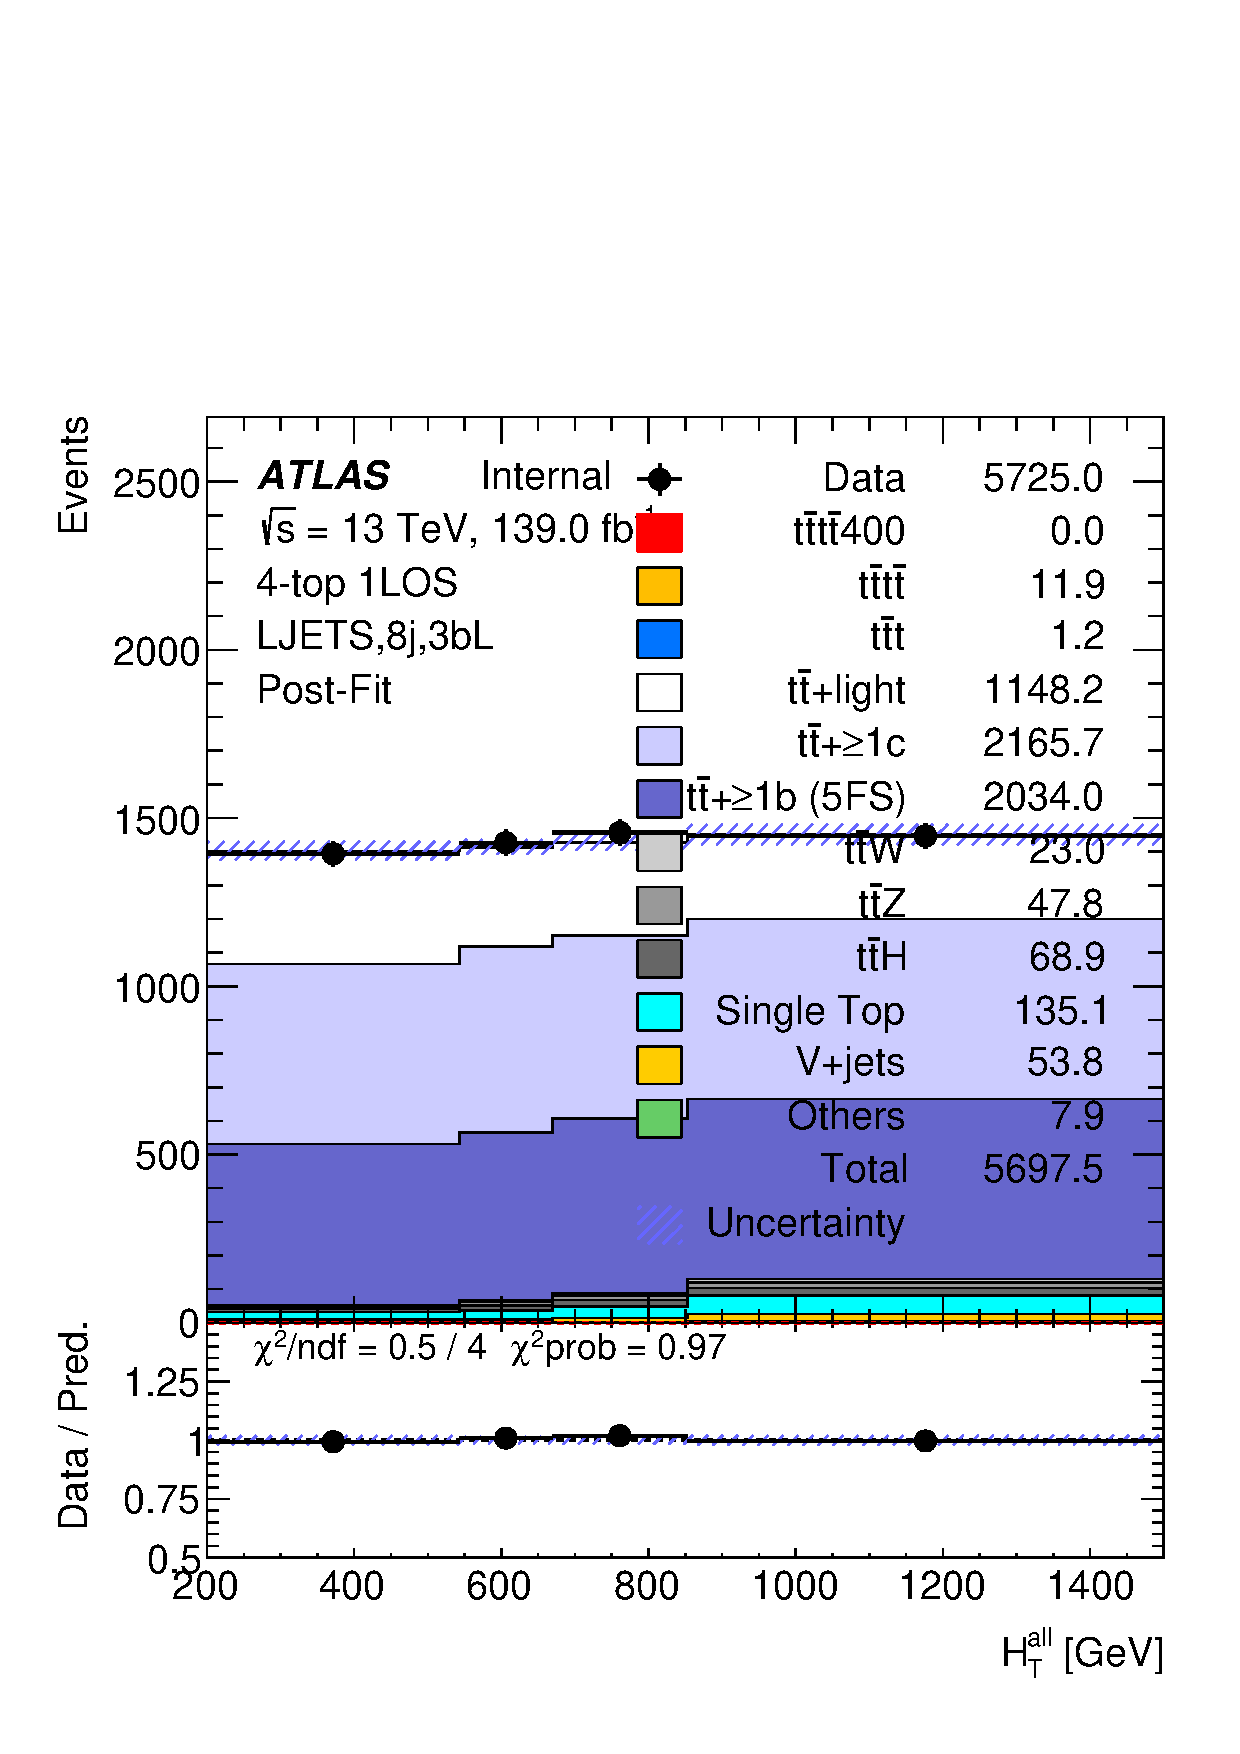
\includegraphics[width=0.23 \textwidth]{figures/fits/GNN/400/all/data_unblindedBonly/Plots/ljets_8j3bL_postFit.pdf} &
        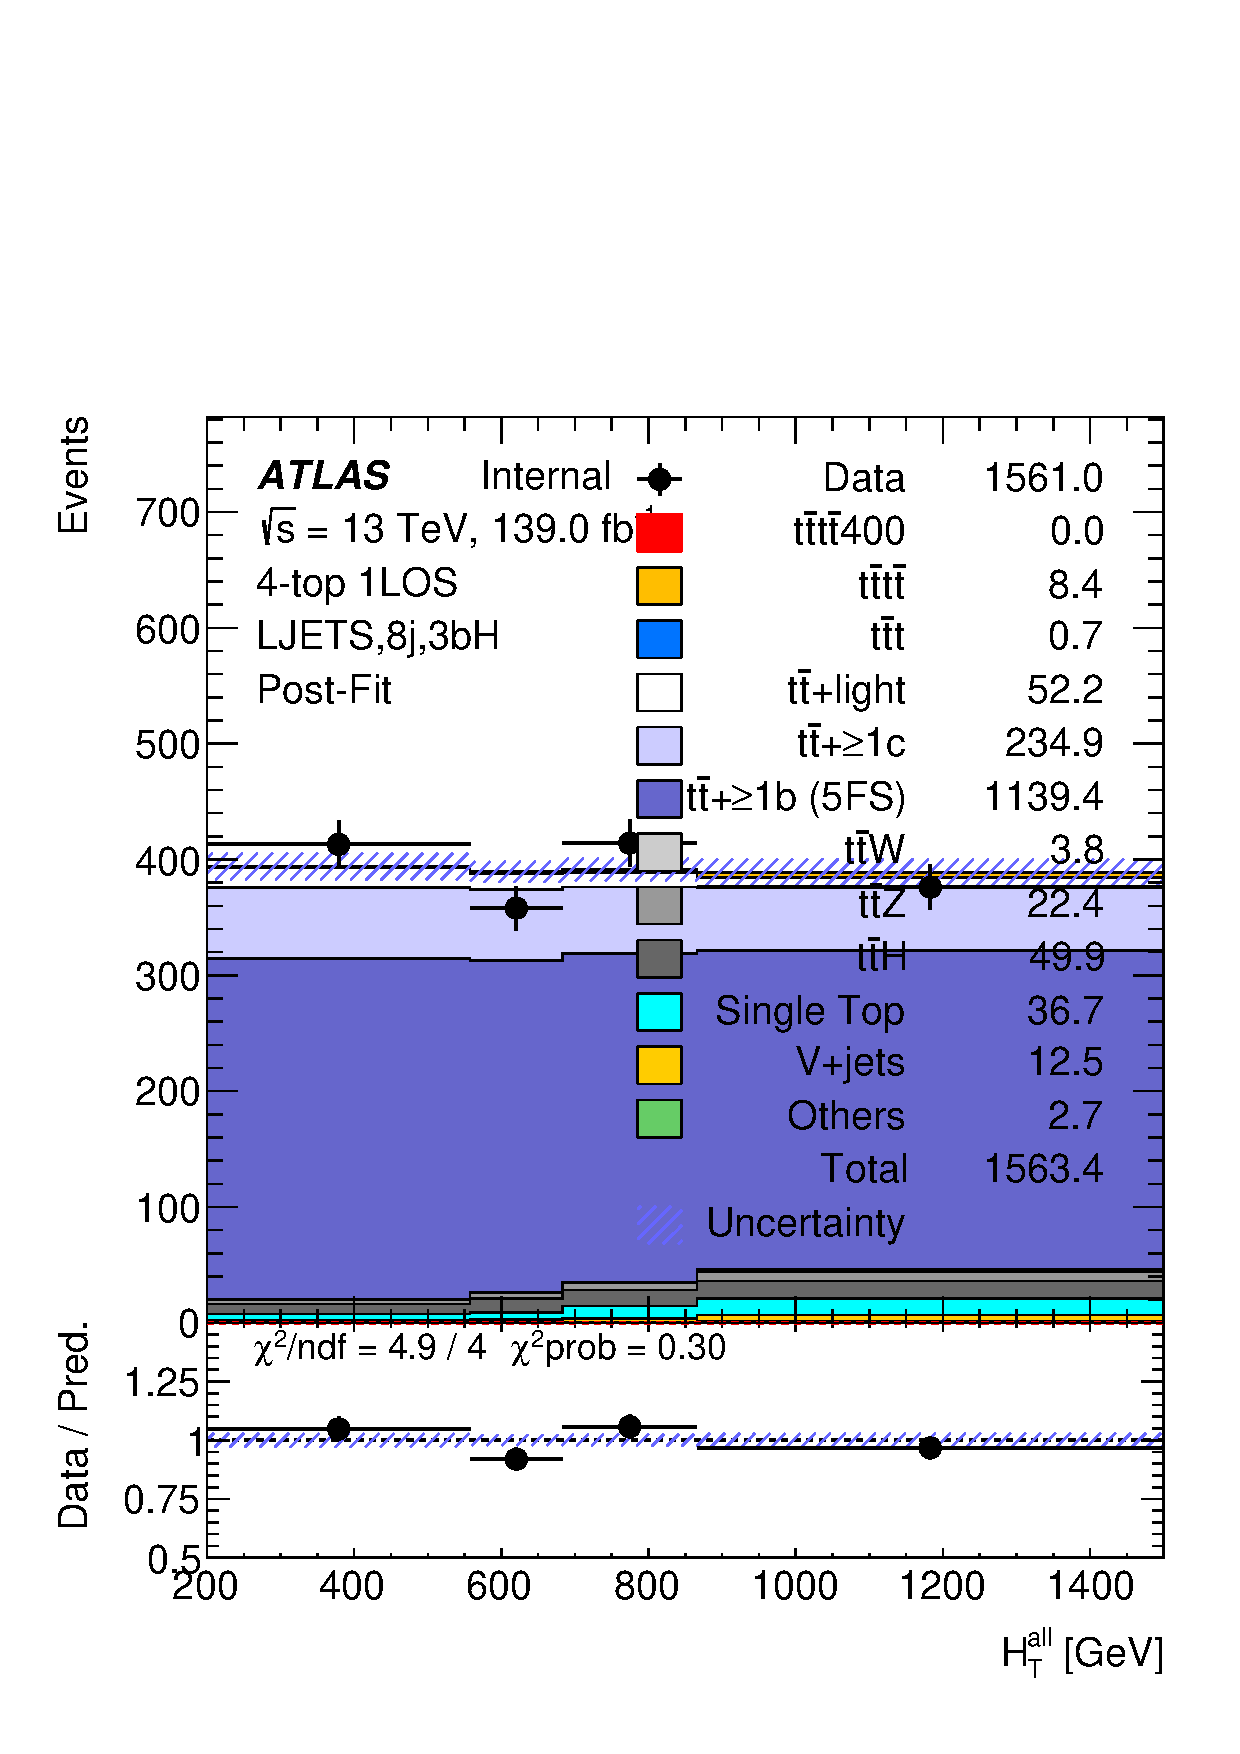
\includegraphics[width=0.23 \textwidth]{figures/fits/GNN/400/all/data_unblindedBonly/Plots/ljets_8j3bH_postFit.pdf} &
        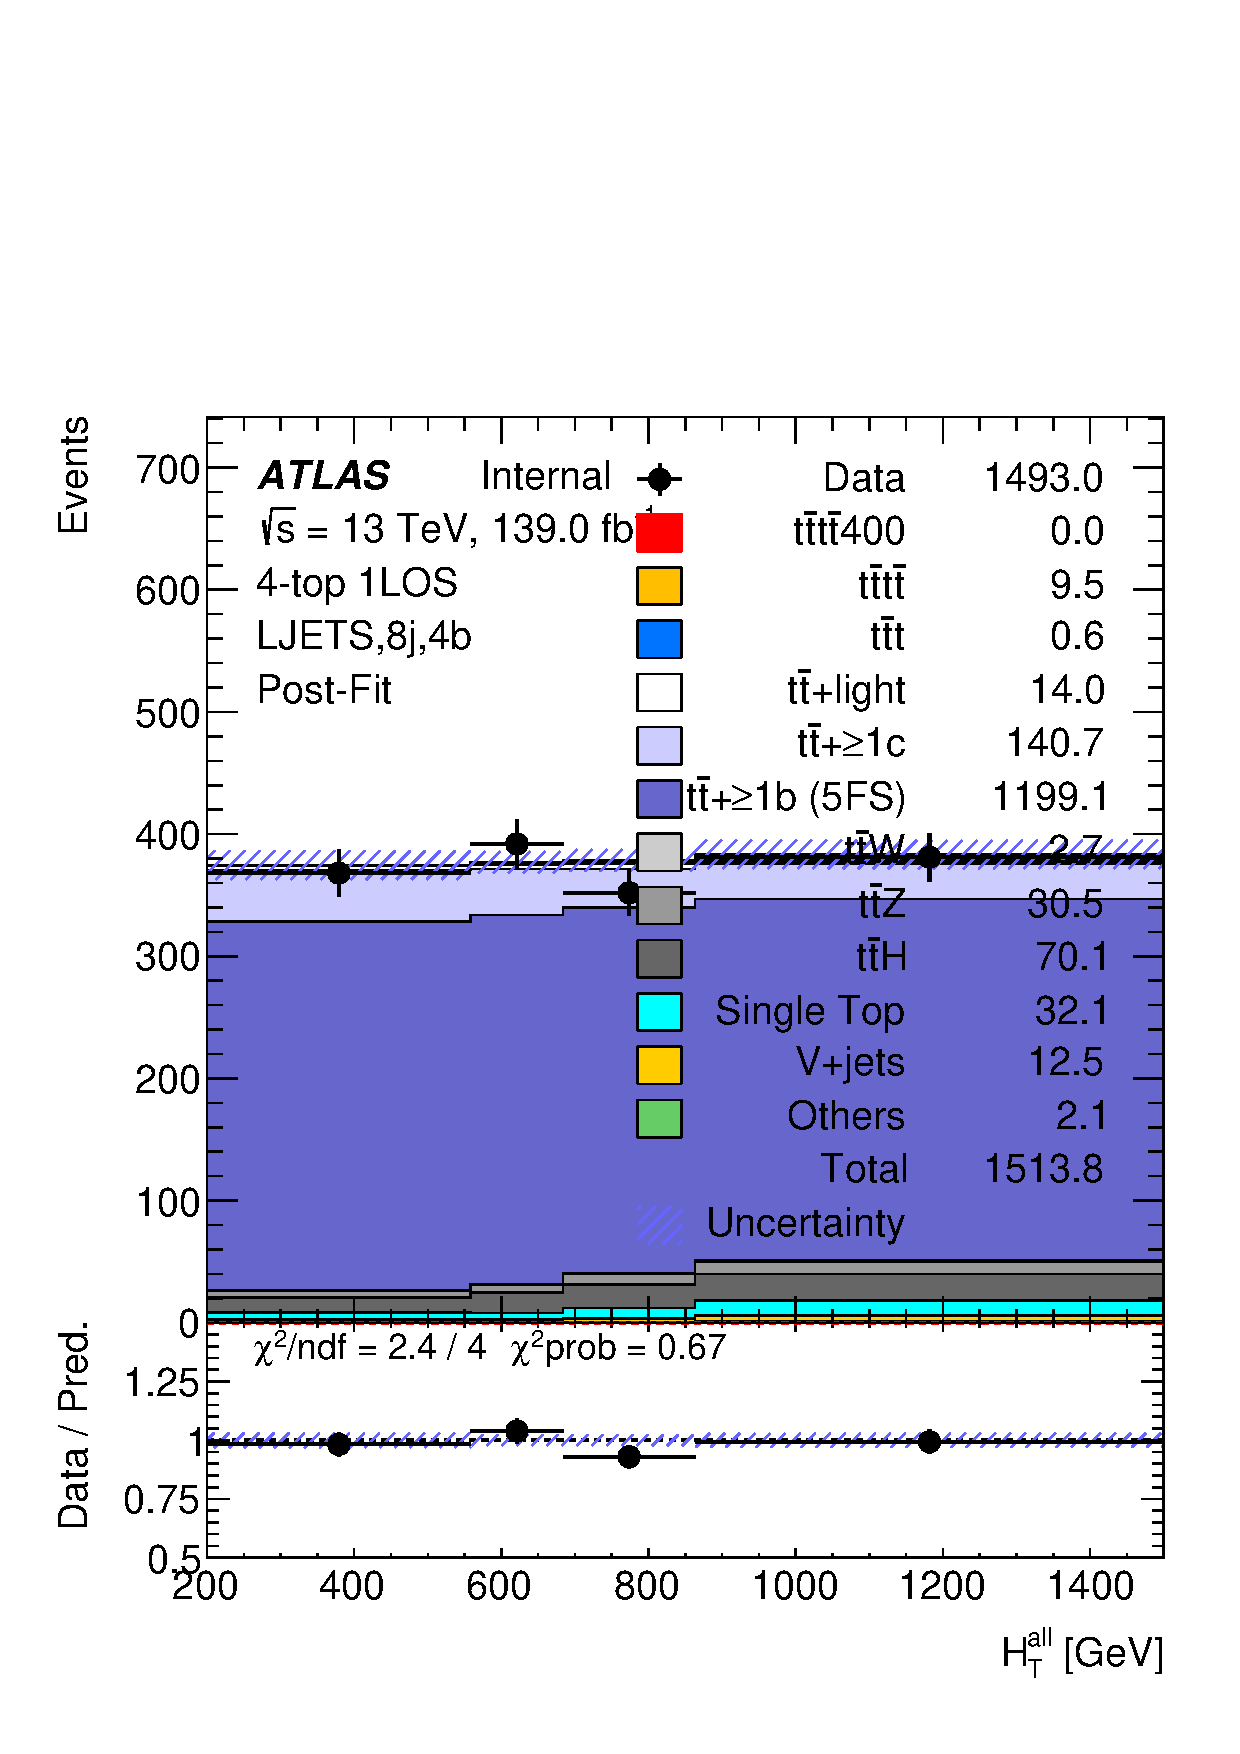
\includegraphics[width=0.23 \textwidth]{figures/fits/GNN/400/all/data_unblindedBonly/Plots/ljets_8j4b_postFit.pdf} &
        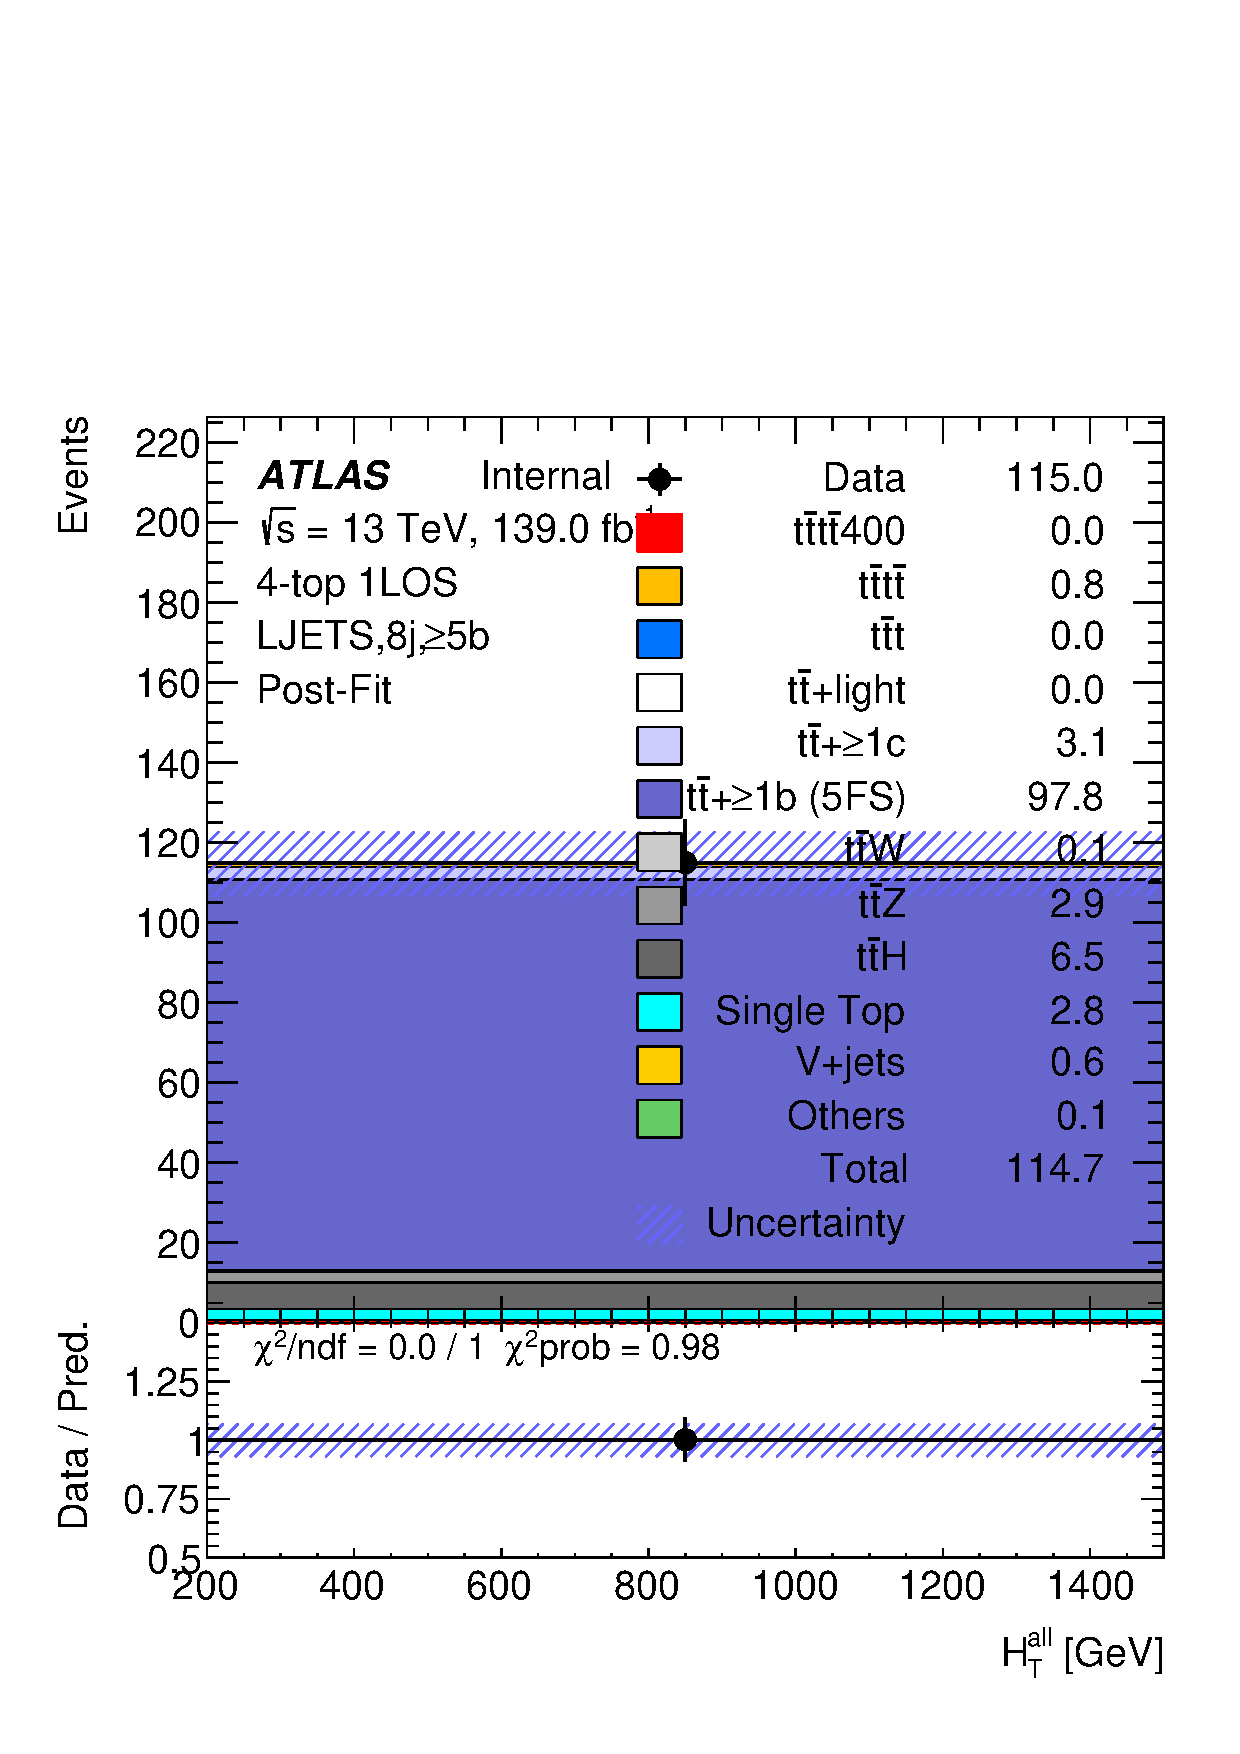
\includegraphics[width=0.23 \textwidth]{figures/fits/GNN/400/all/data_unblindedBonly/Plots/ljets_8jge5b_postFit.pdf}\\

        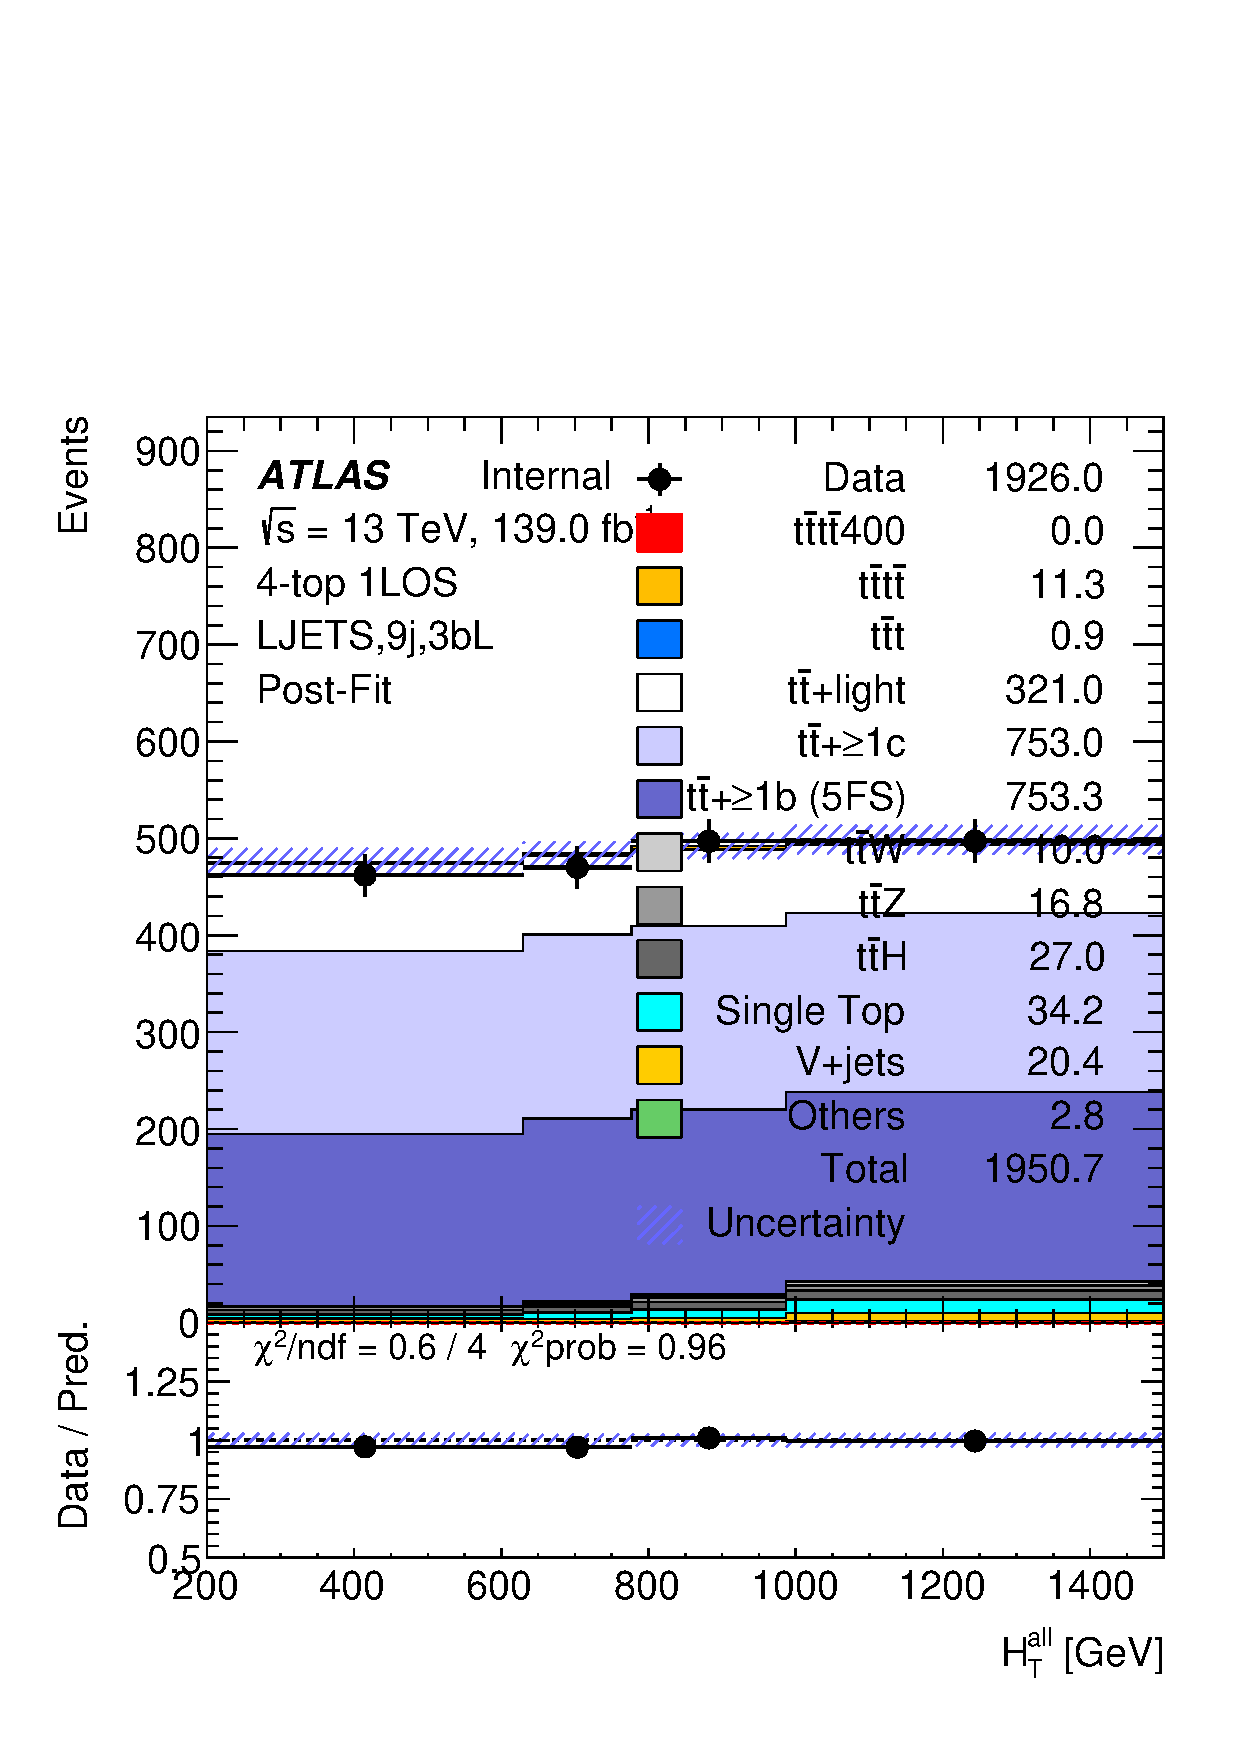
\includegraphics[width=0.23 \textwidth]{figures/fits/GNN/400/all/data_unblindedBonly/Plots/ljets_9j3bL_postFit.pdf} &
        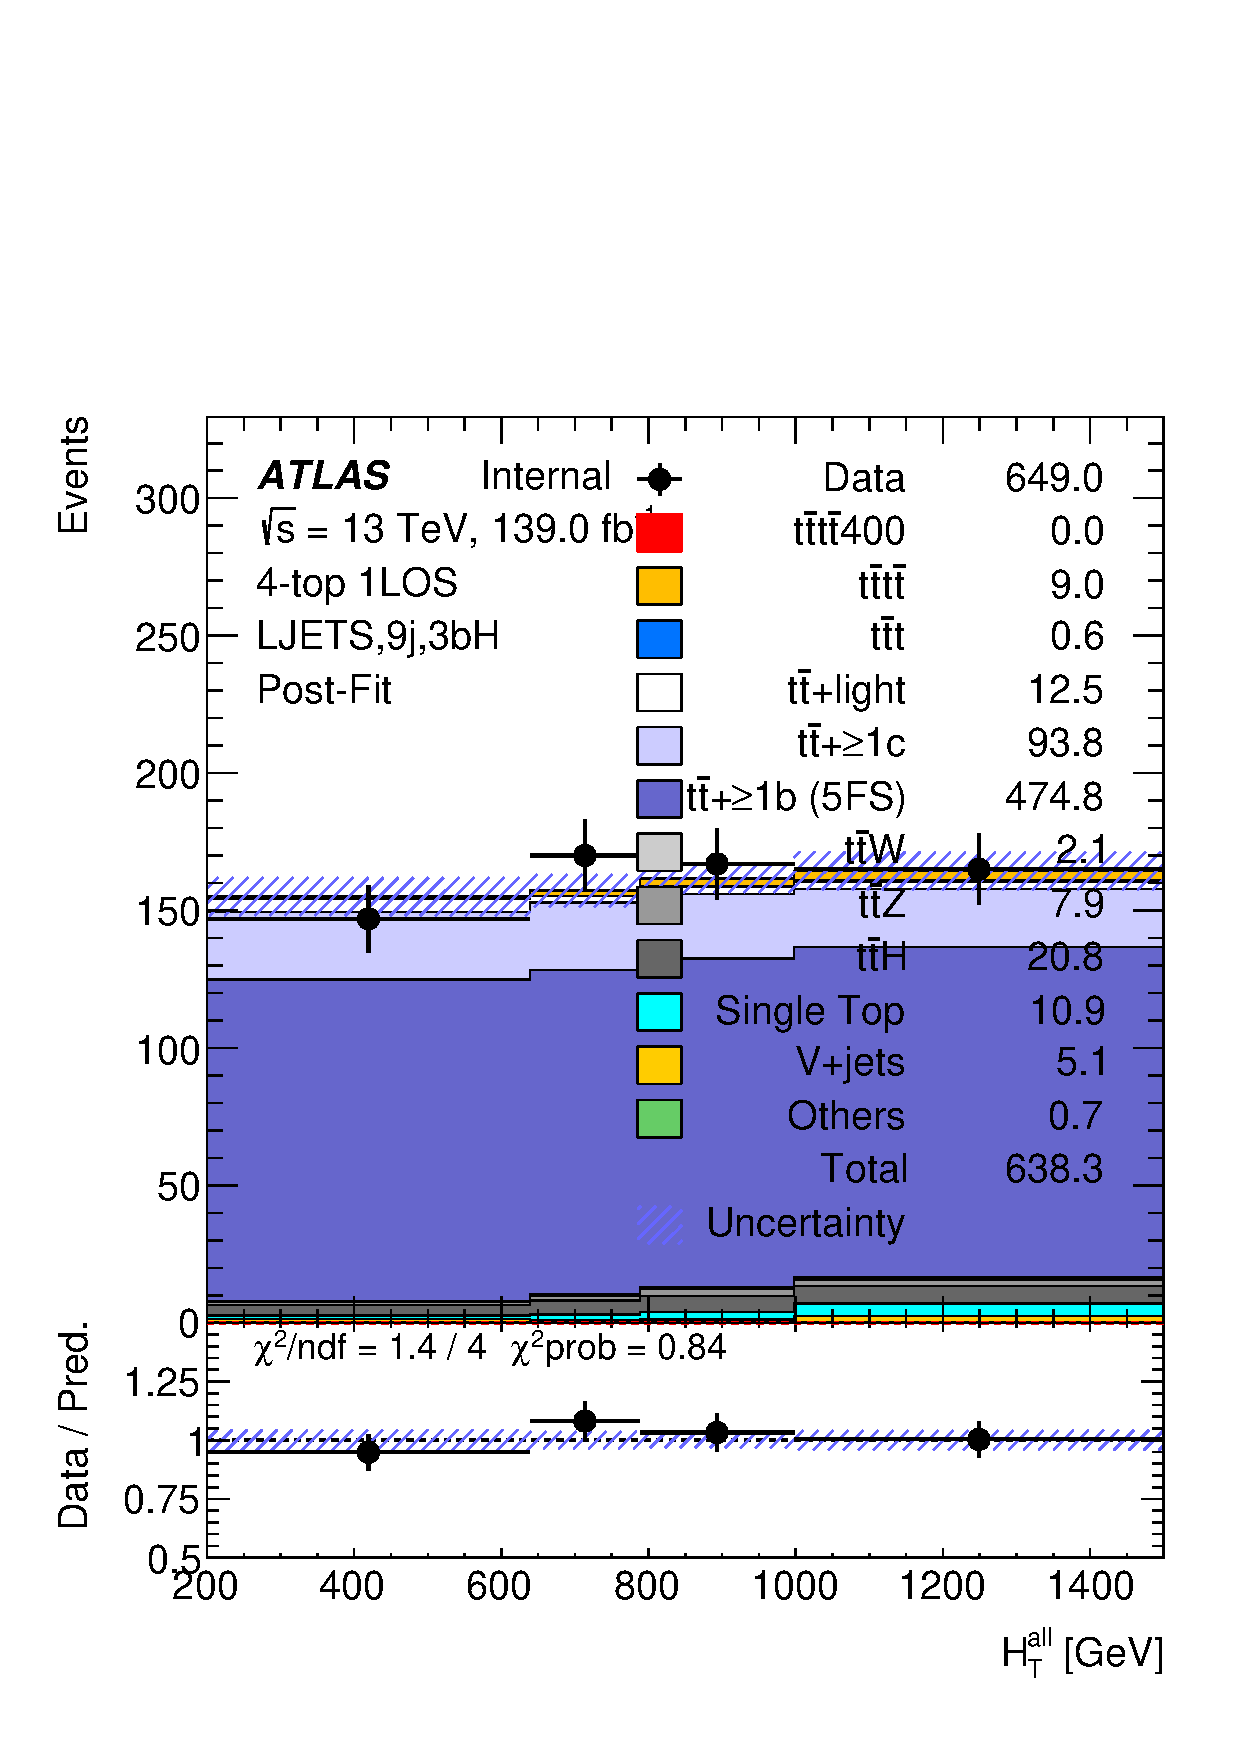
\includegraphics[width=0.23 \textwidth]{figures/fits/GNN/400/all/data_unblindedBonly/Plots/ljets_9j3bH_postFit.pdf} &
        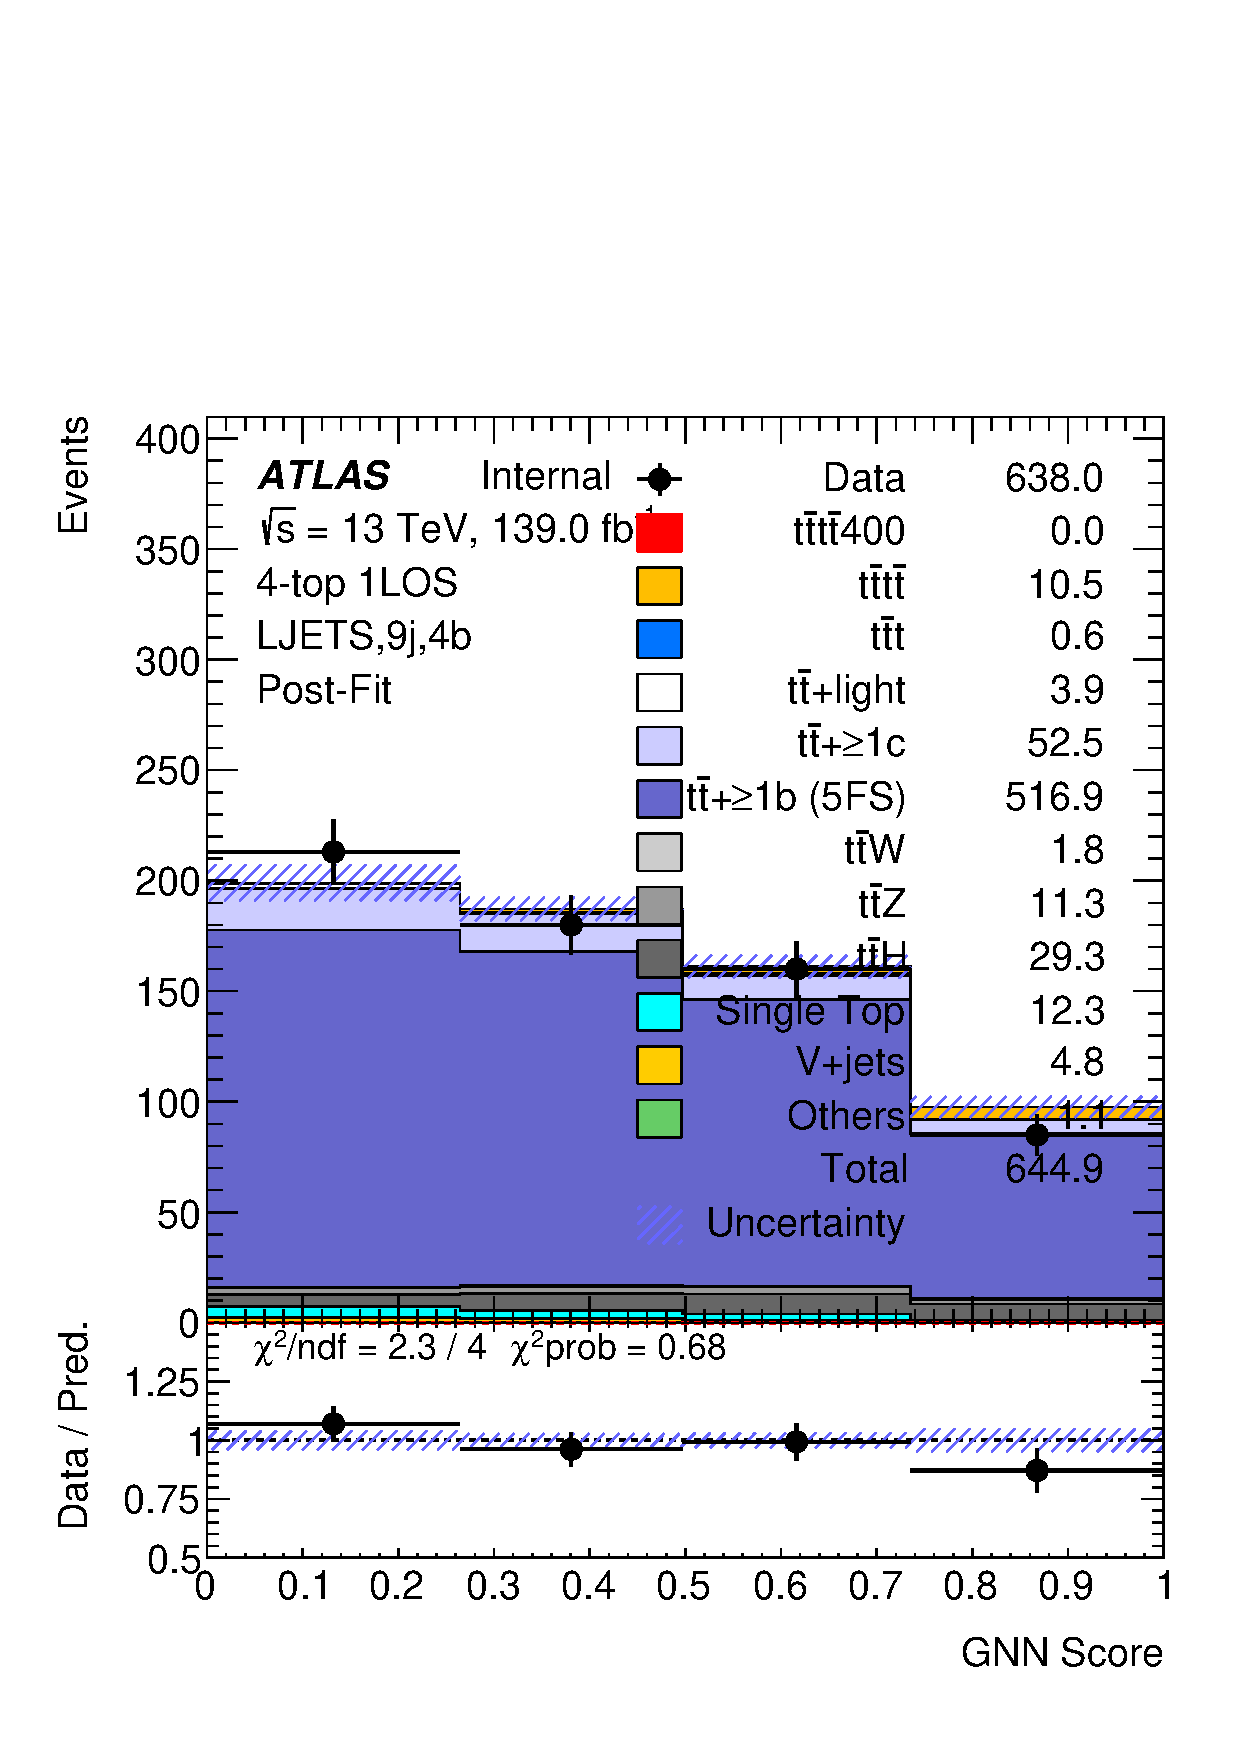
\includegraphics[width=0.23 \textwidth]{figures/fits/GNN/400/all/data_unblindedBonly/Plots/ljets_9j4b_postFit.pdf} &
        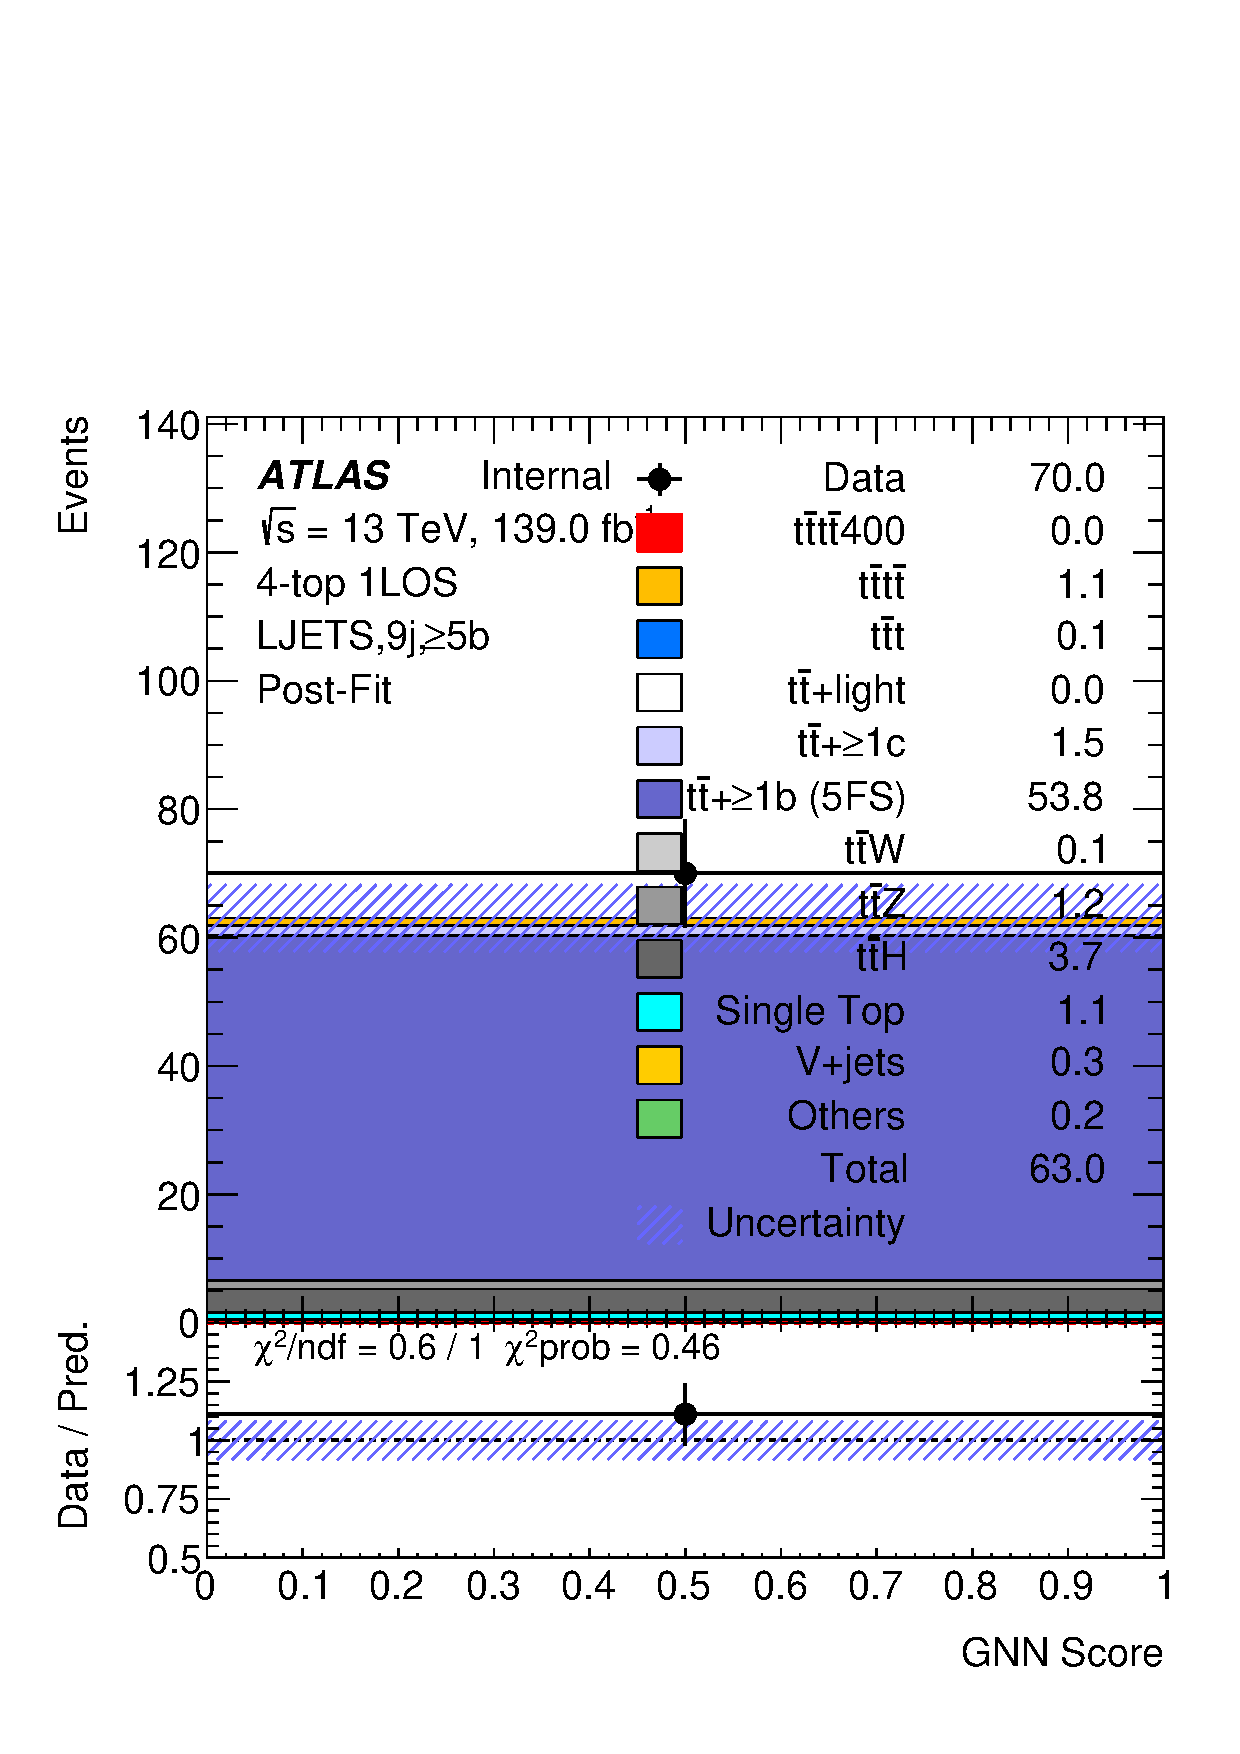
\includegraphics[width=0.23 \textwidth]{figures/fits/GNN/400/all/data_unblindedBonly/Plots/ljets_9jge5b_postFit.pdf} \\

        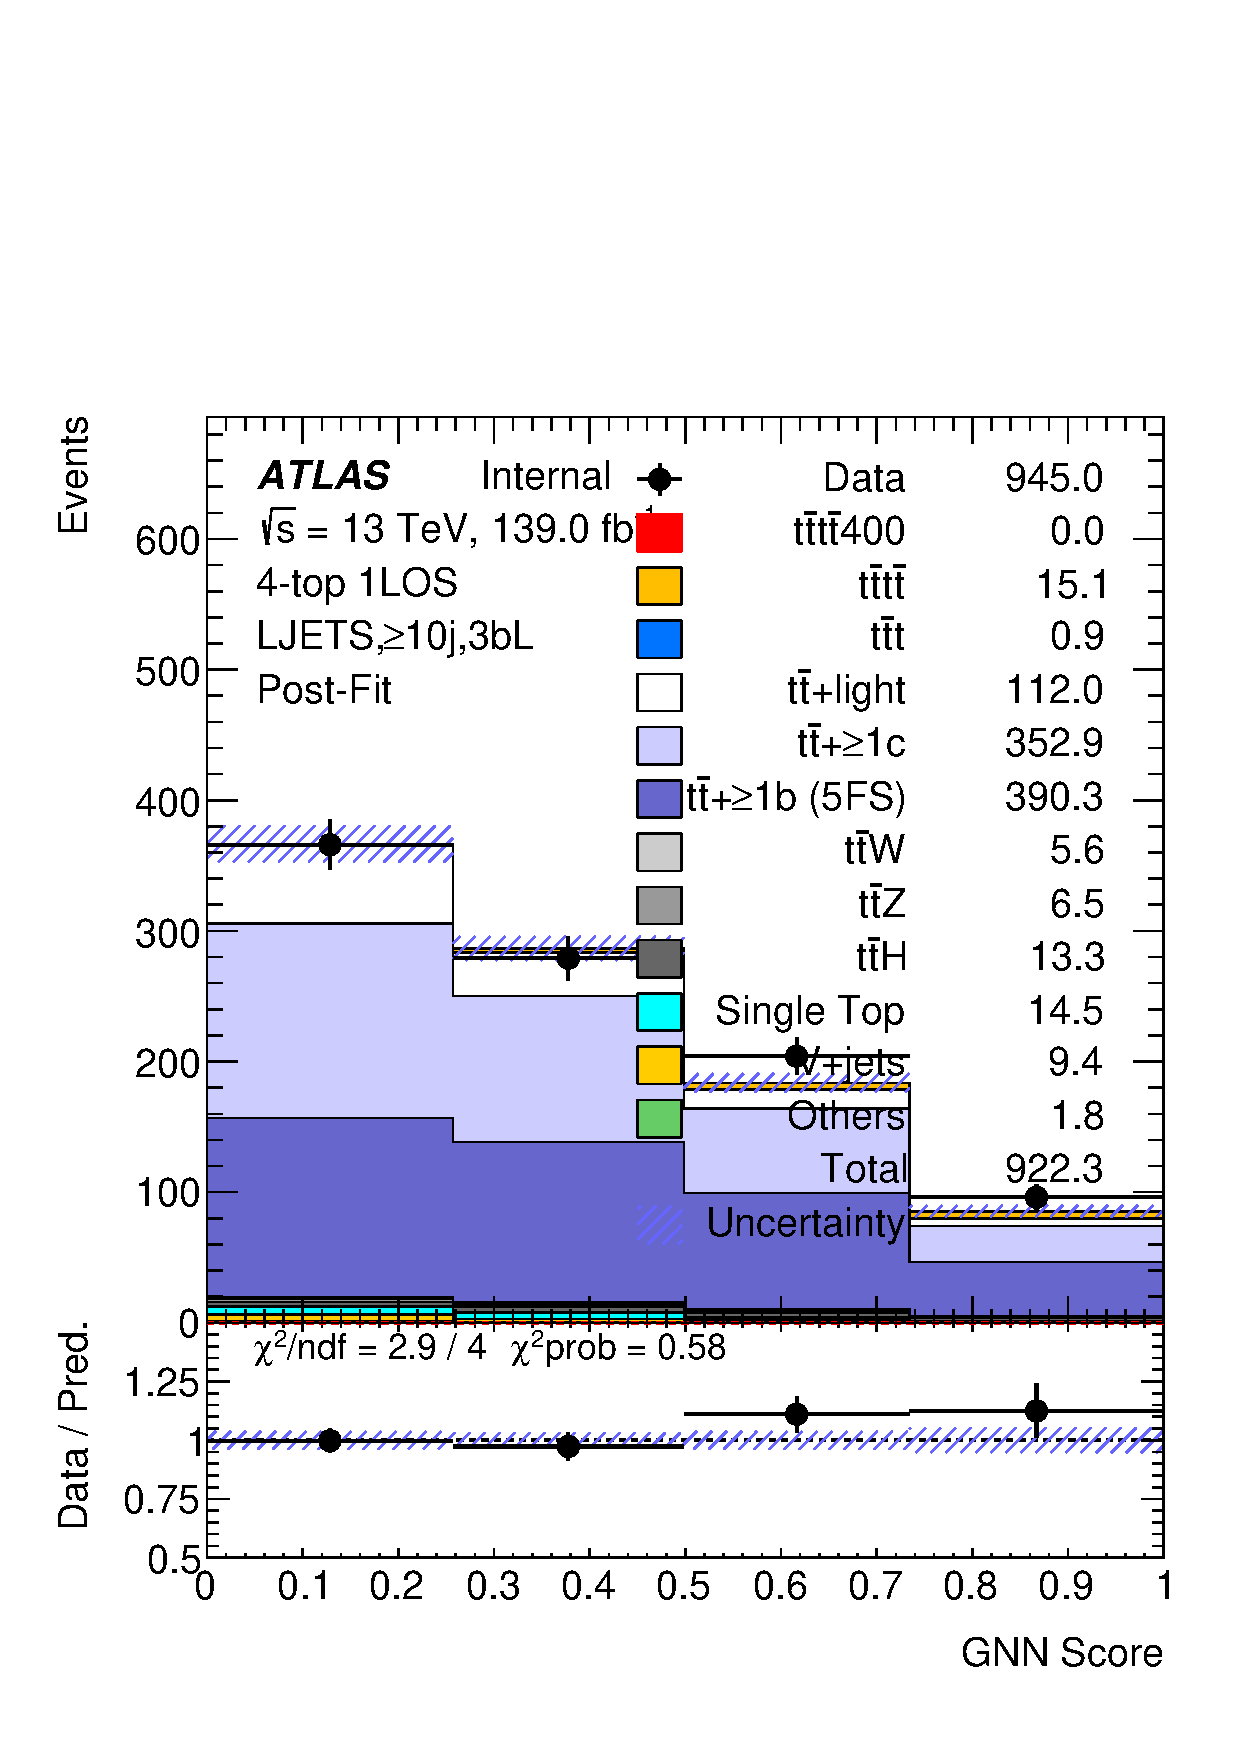
\includegraphics[width=0.23 \textwidth]{figures/fits/GNN/400/all/data_unblindedBonly/Plots/ljets_ge10j3bL_postFit.pdf} &
        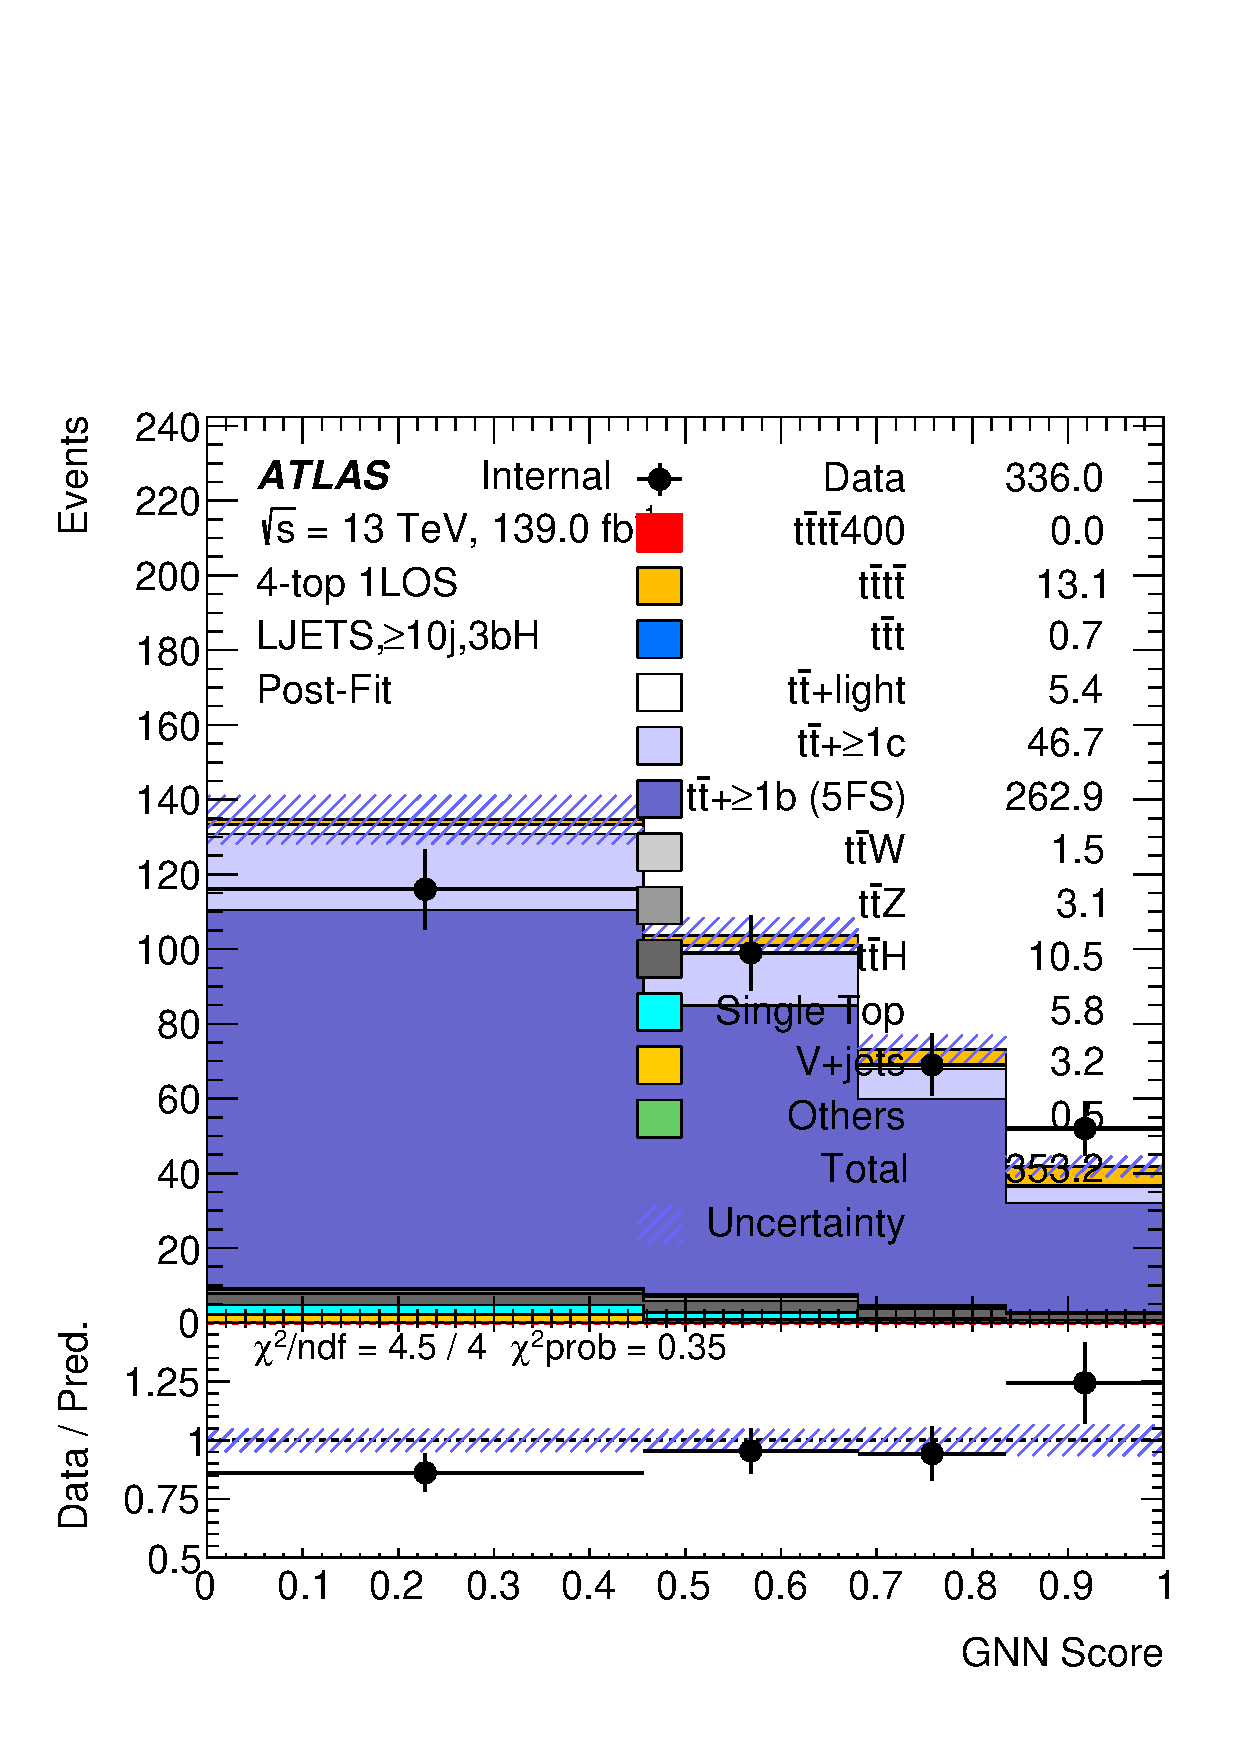
\includegraphics[width=0.23 \textwidth]{figures/fits/GNN/400/all/data_unblindedBonly/Plots/ljets_ge10j3bH_postFit.pdf} &
        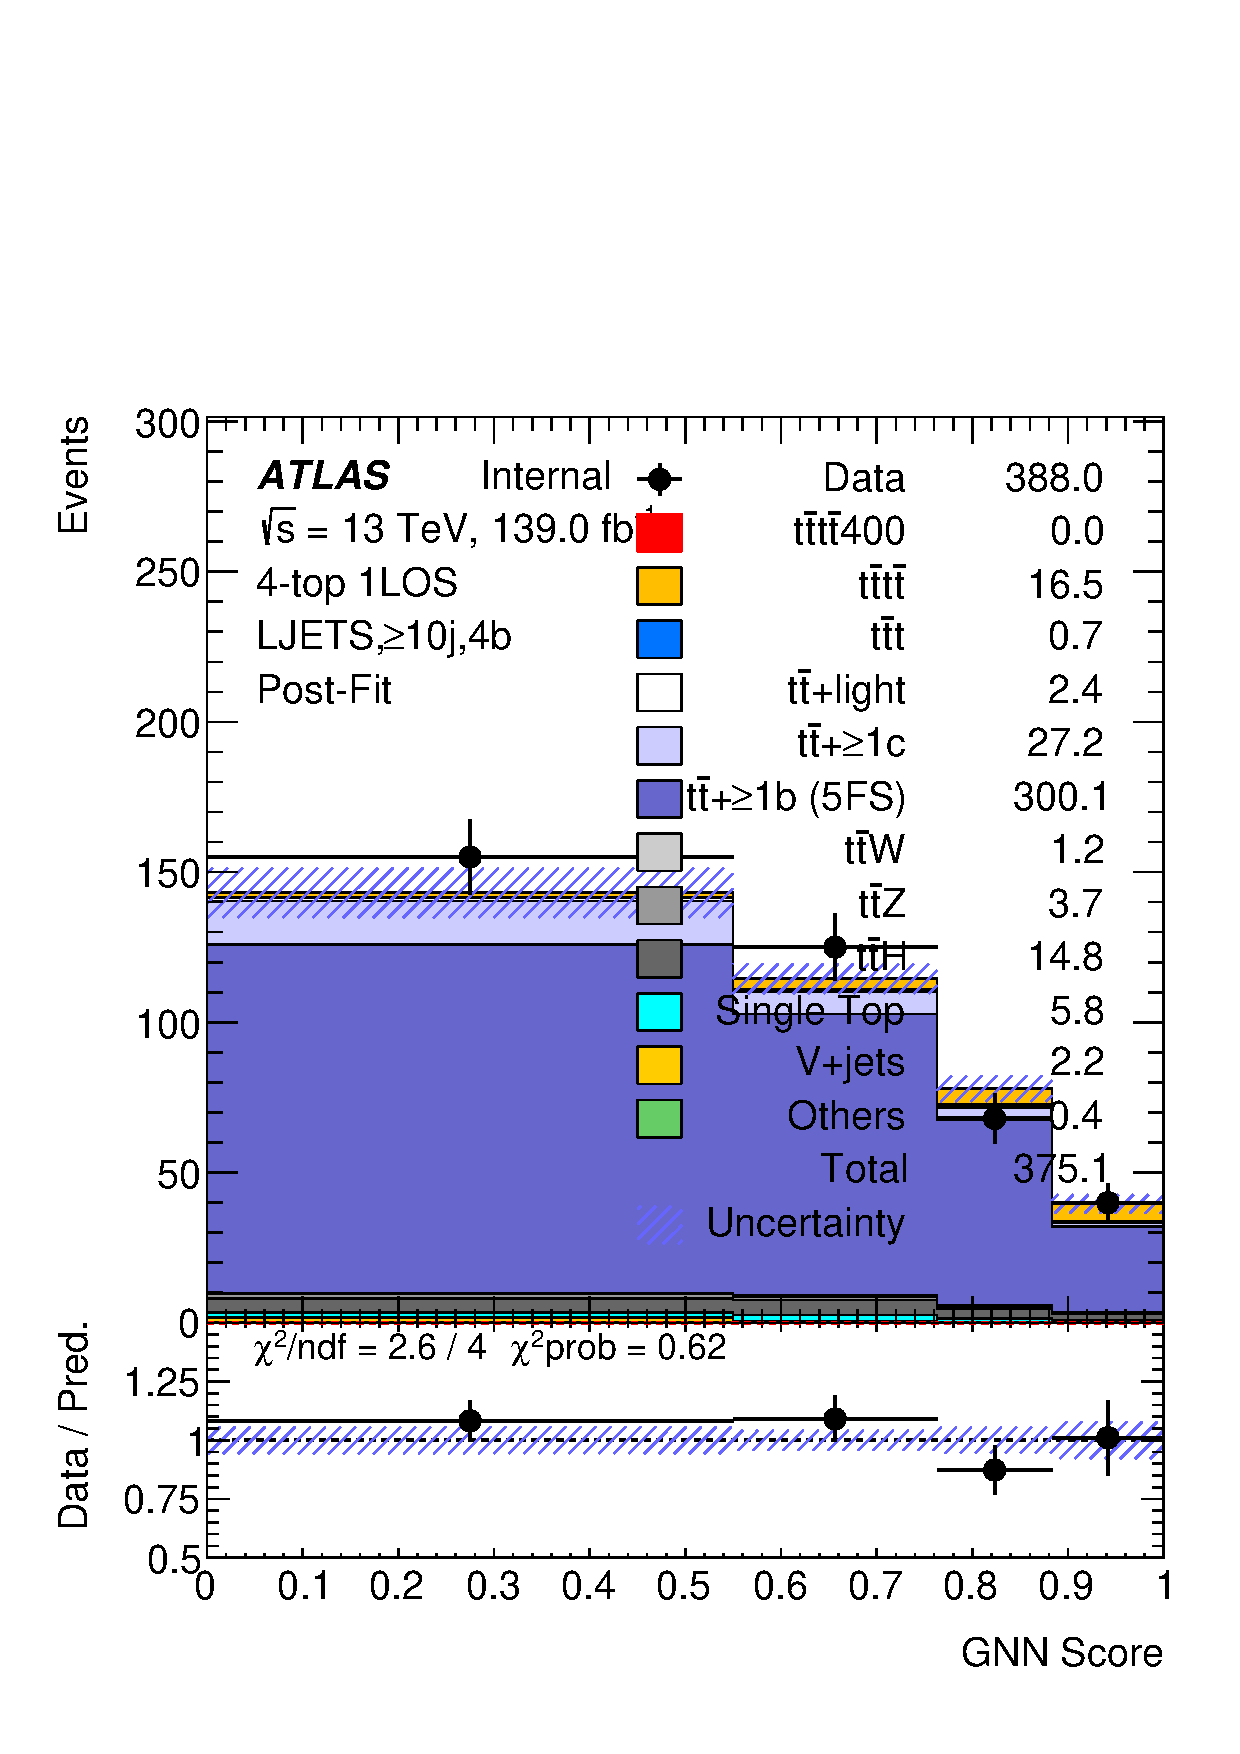
\includegraphics[width=0.23 \textwidth]{figures/fits/GNN/400/all/data_unblindedBonly/Plots/ljets_ge10j4b_postFit.pdf} &
        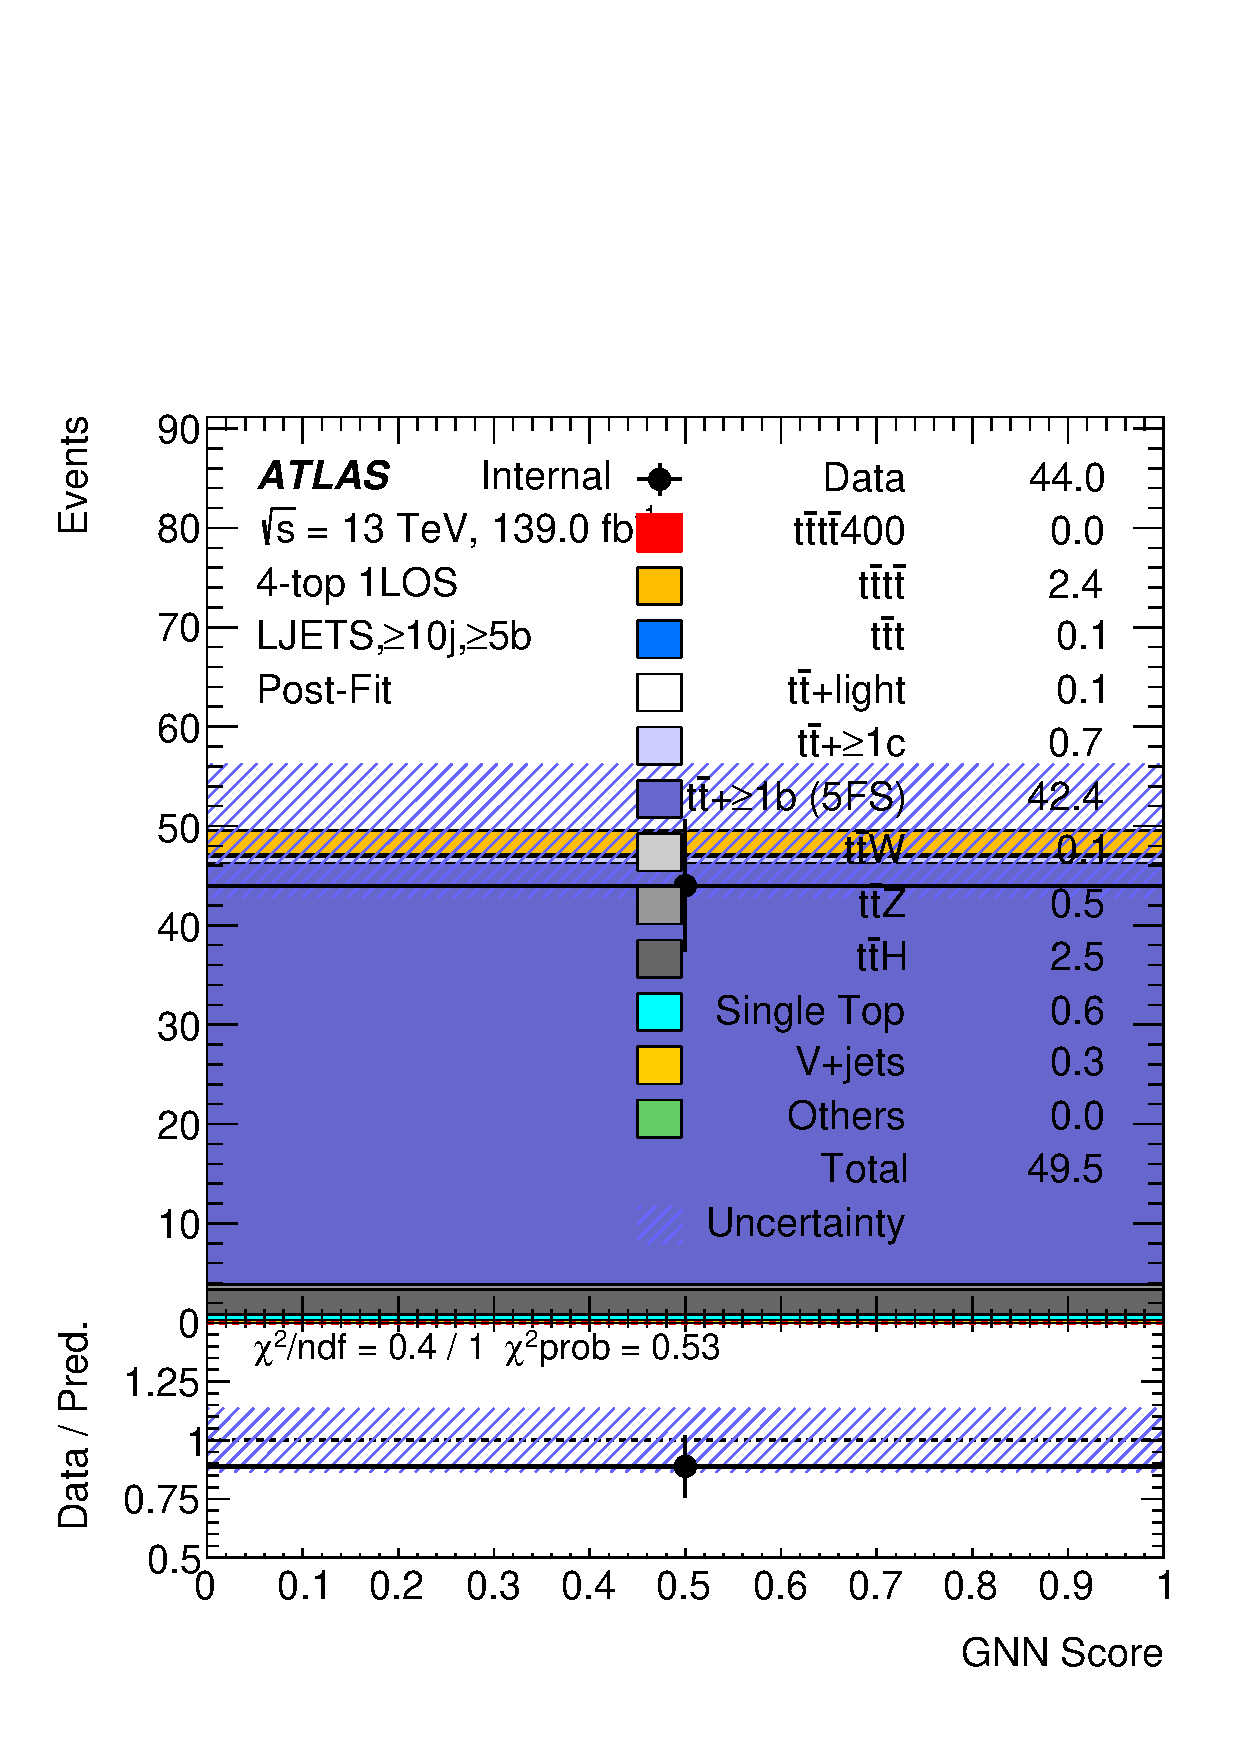
\includegraphics[width=0.23 \textwidth]{figures/fits/GNN/400/all/data_unblindedBonly/Plots/ljets_ge10jge5b_postFit.pdf} \\
        \end{tabular}
        \caption{\label{fig:unblinded_data_Bonly_postfit_1L}
        Post-fit distributions for the 1L regions obtained from the background-only unblinded data fit at $\boldsymbol{m_H=400}$~GeV. 
        The fit is performed using all regions (1L+2LOS).}
\end{center}
\end{figure}

% -----------------------------
% 2L post-fit
% -----------------------------
\begin{figure}[htbp!]
        \begin{center} \setlength{\tabcolsep}{2.5pt}\footnotesize
        \begin{tabular}{ccc}
        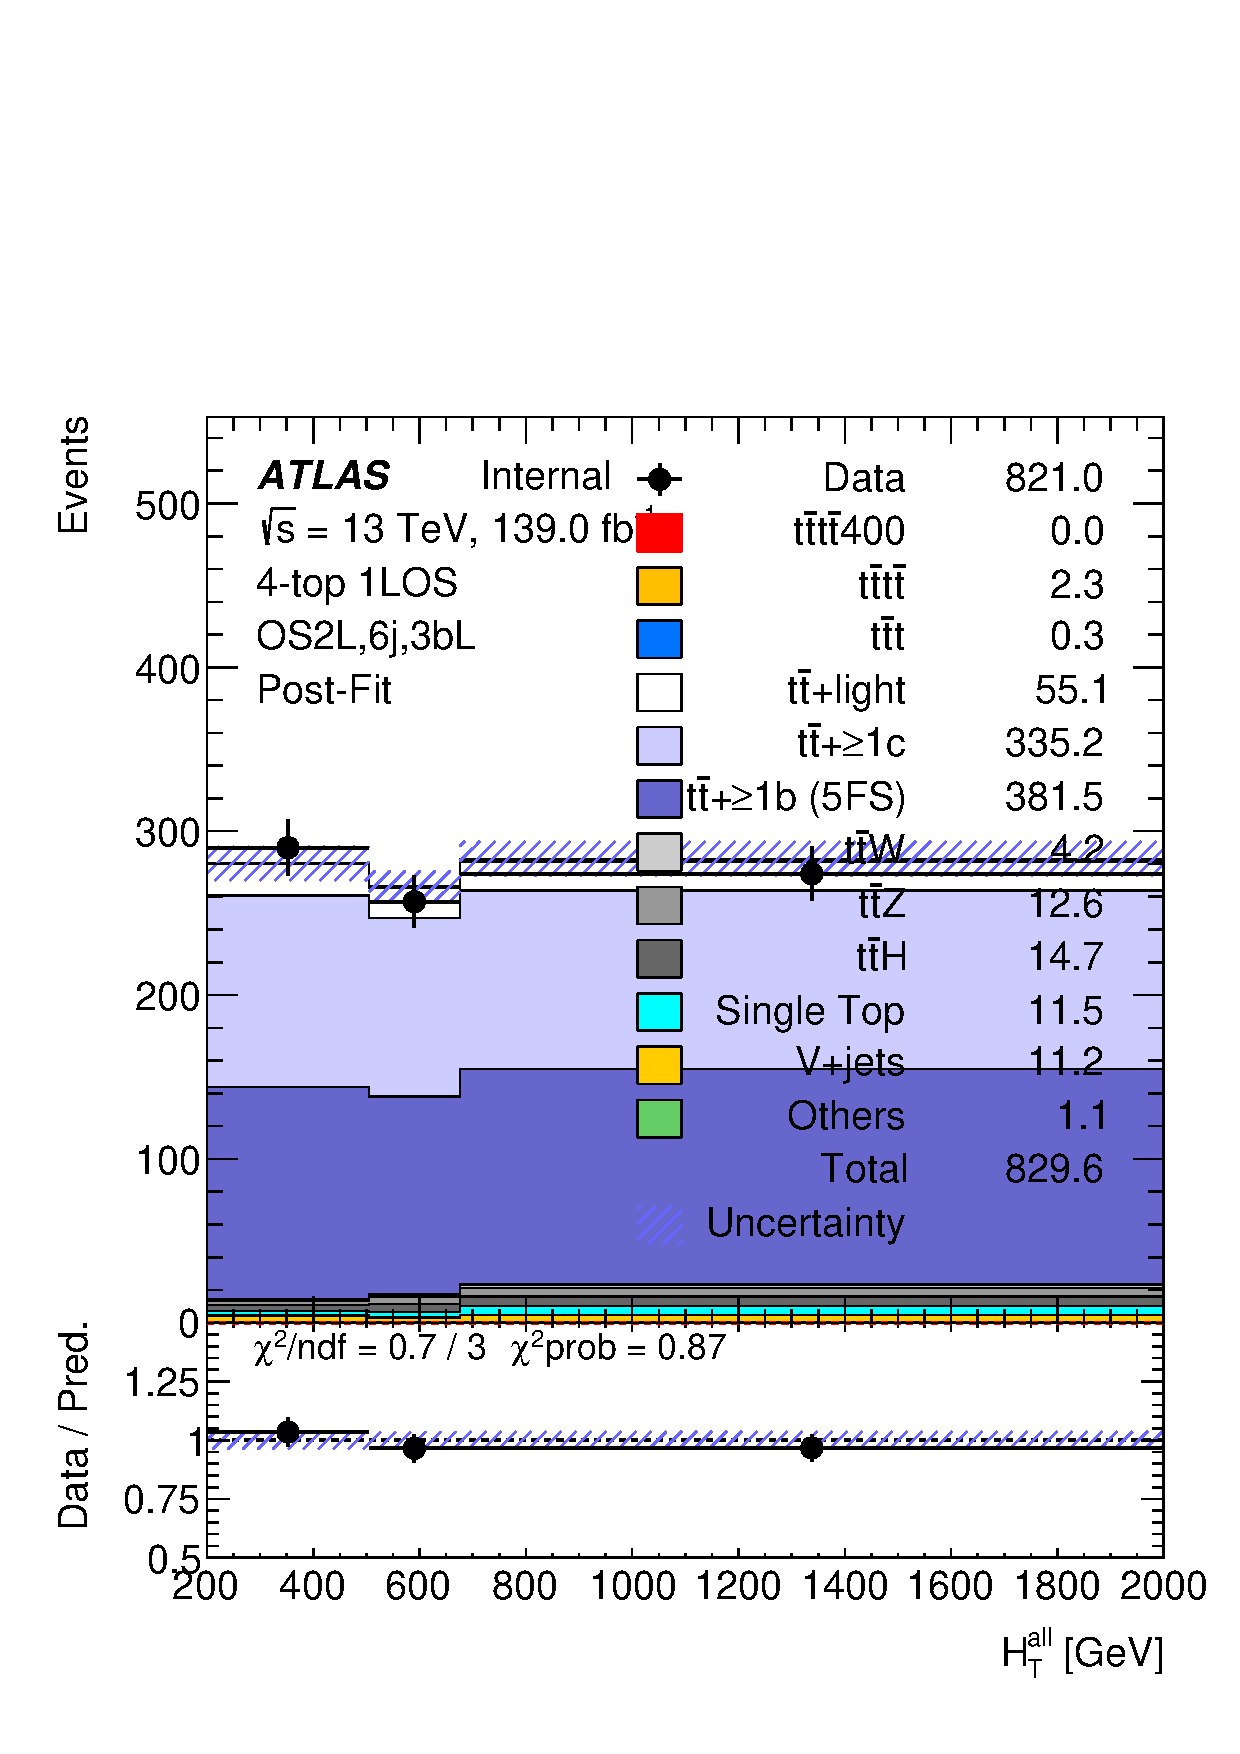
\includegraphics[width=0.31 \textwidth]{figures/fits/GNN/400/all/data_unblindedBonly/Plots/os2l_6j3bL_postFit.pdf} &
        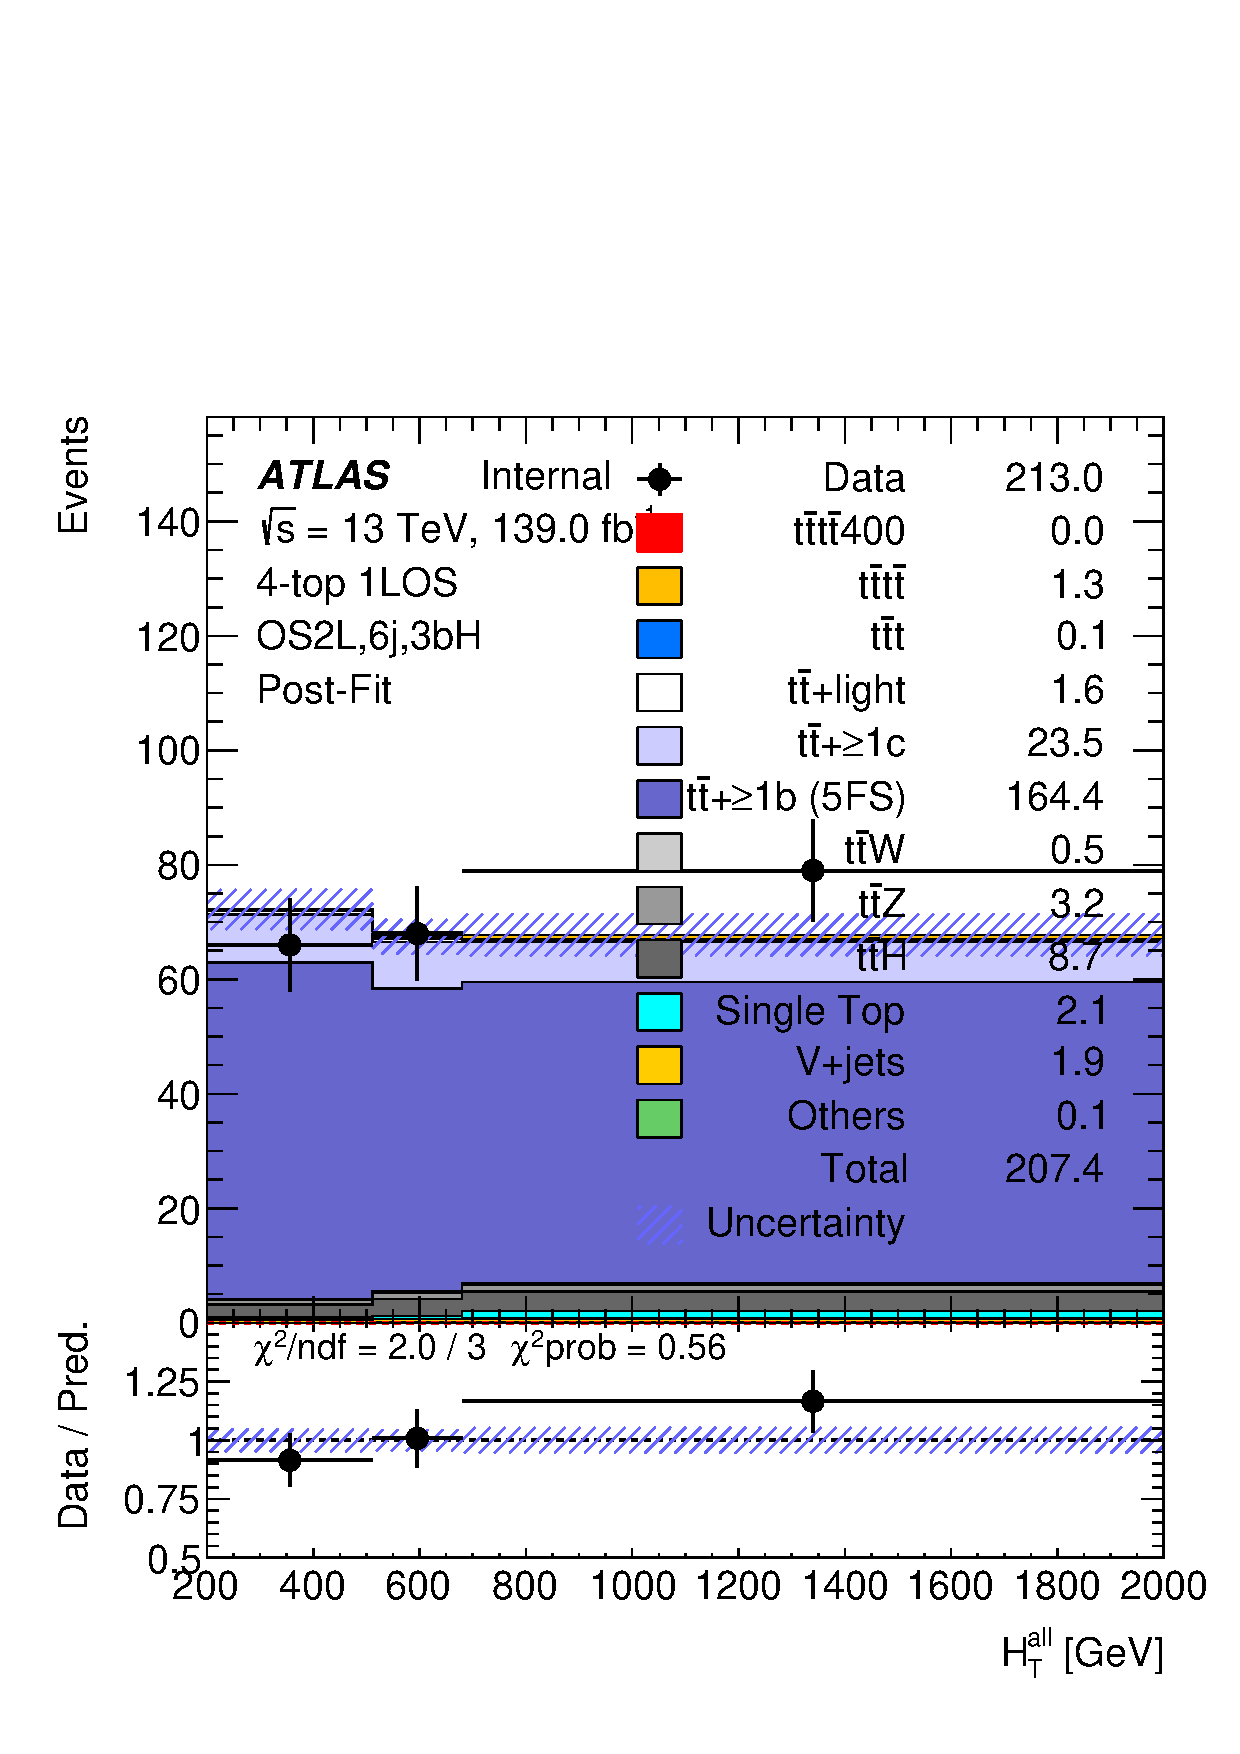
\includegraphics[width=0.31 \textwidth]{figures/fits/GNN/400/all/data_unblindedBonly/Plots/os2l_6j3bH_postFit.pdf} &
        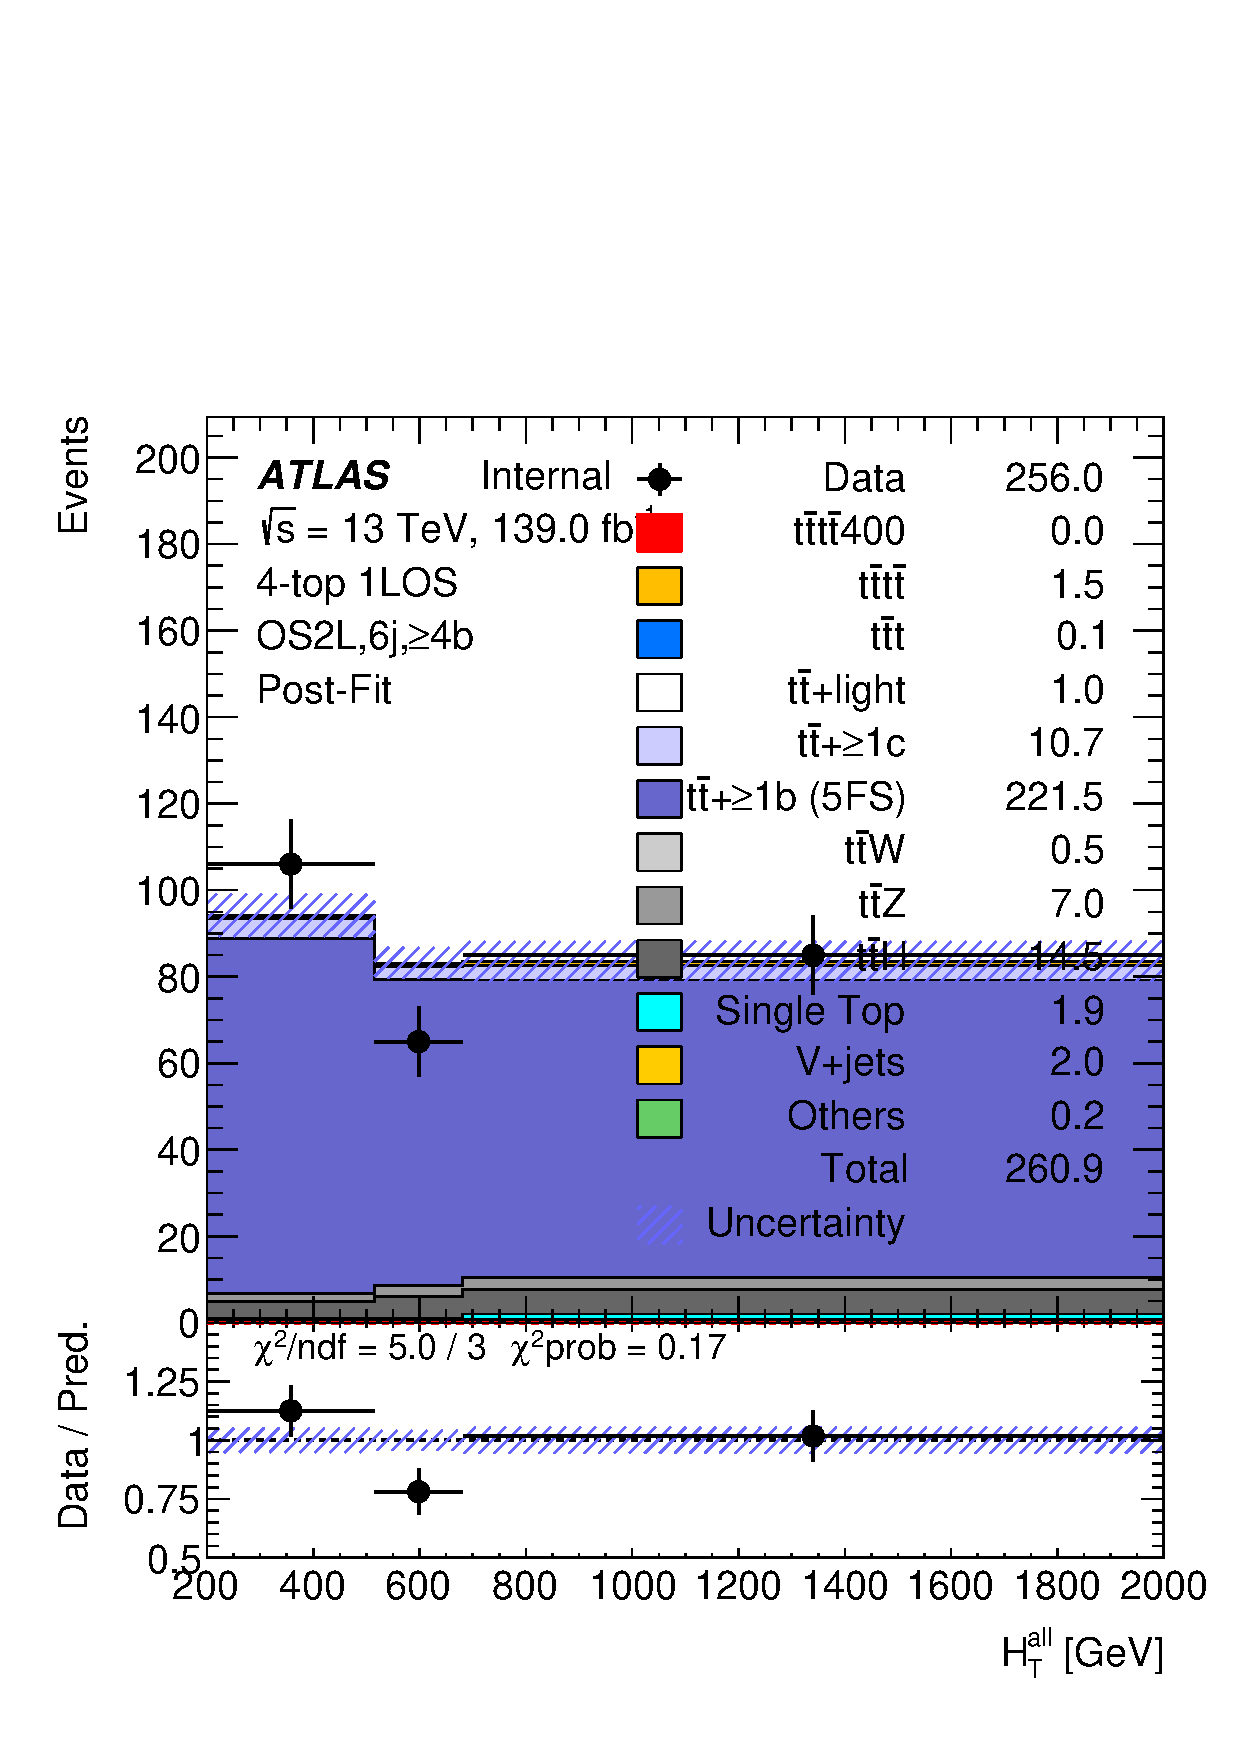
\includegraphics[width=0.31 \textwidth]{figures/fits/GNN/400/all/data_unblindedBonly/Plots/os2l_6jge4b_postFit.pdf} \\

        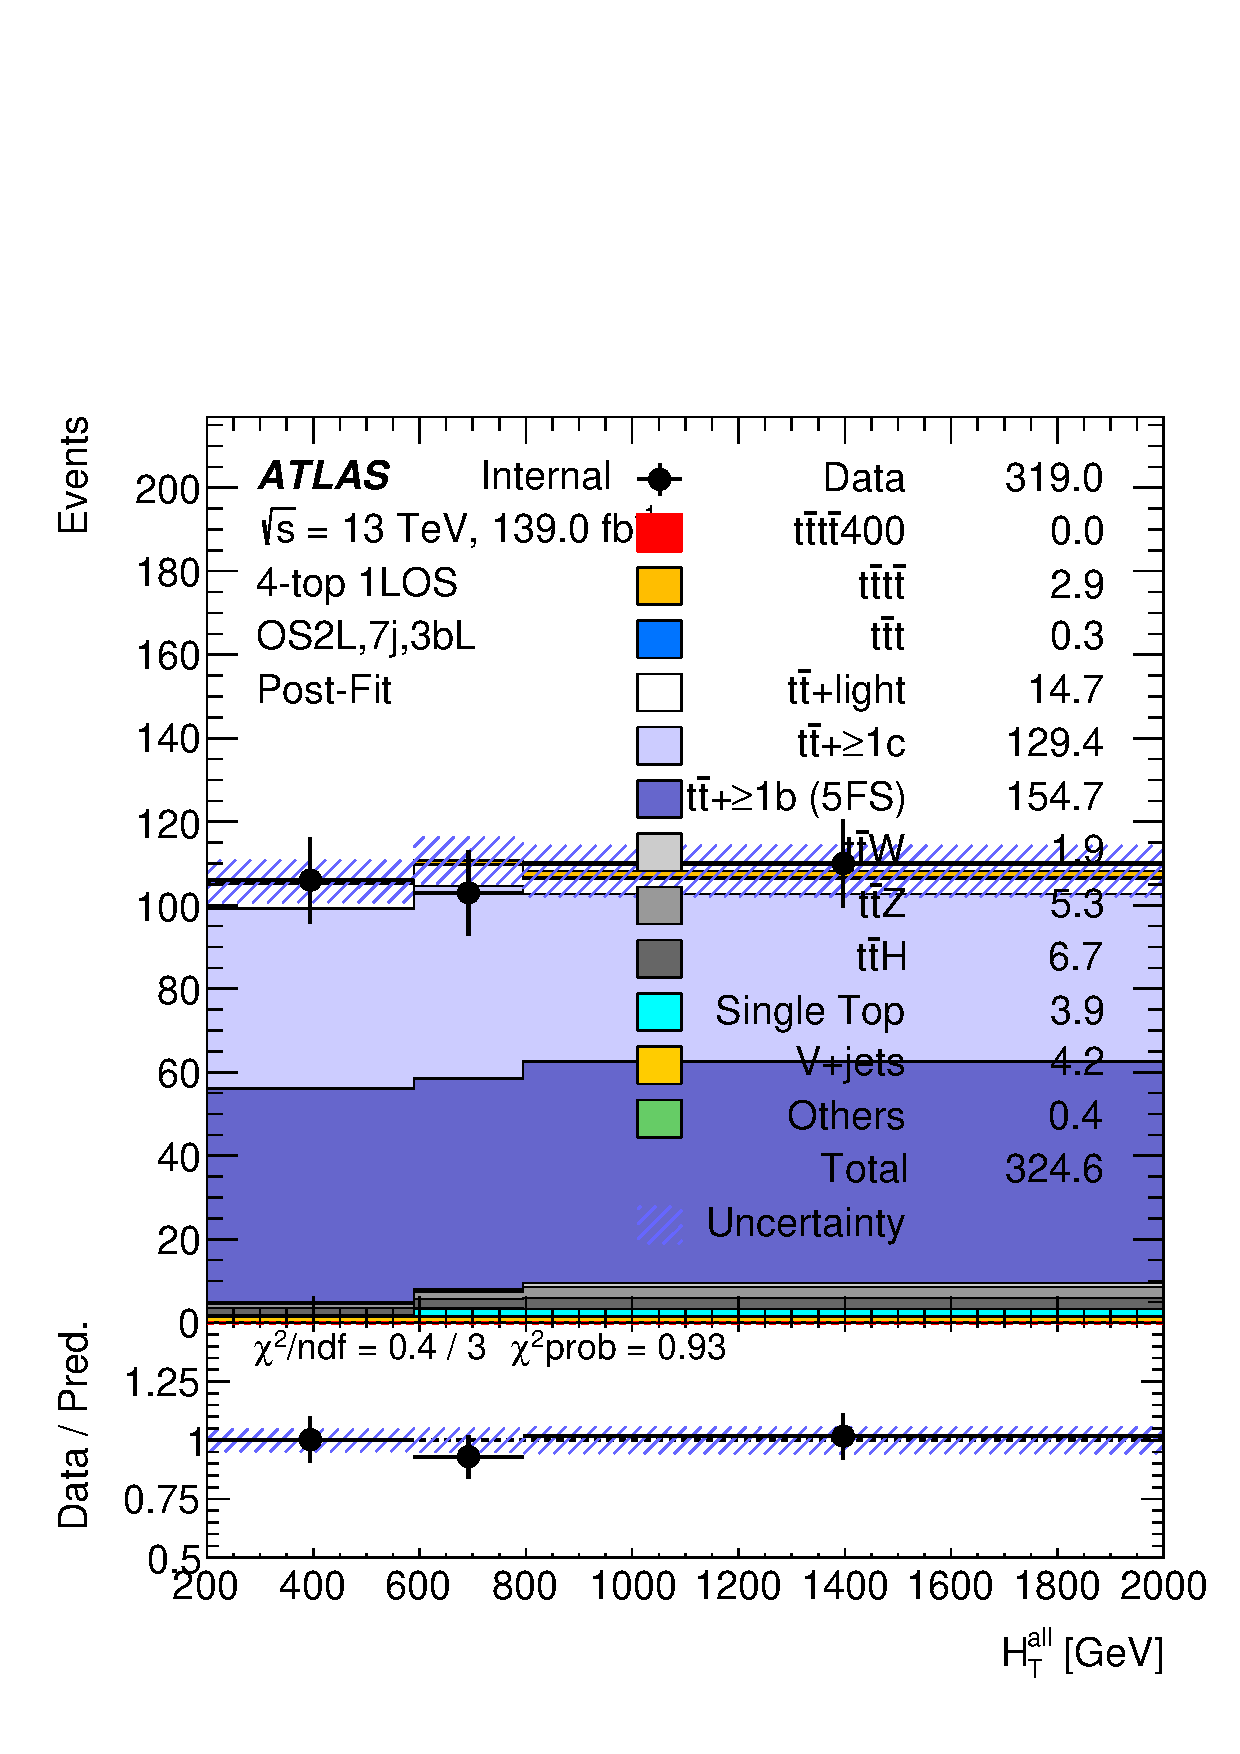
\includegraphics[width=0.31 \textwidth]{figures/fits/GNN/400/all/data_unblindedBonly/Plots/os2l_7j3bL_postFit.pdf} &
        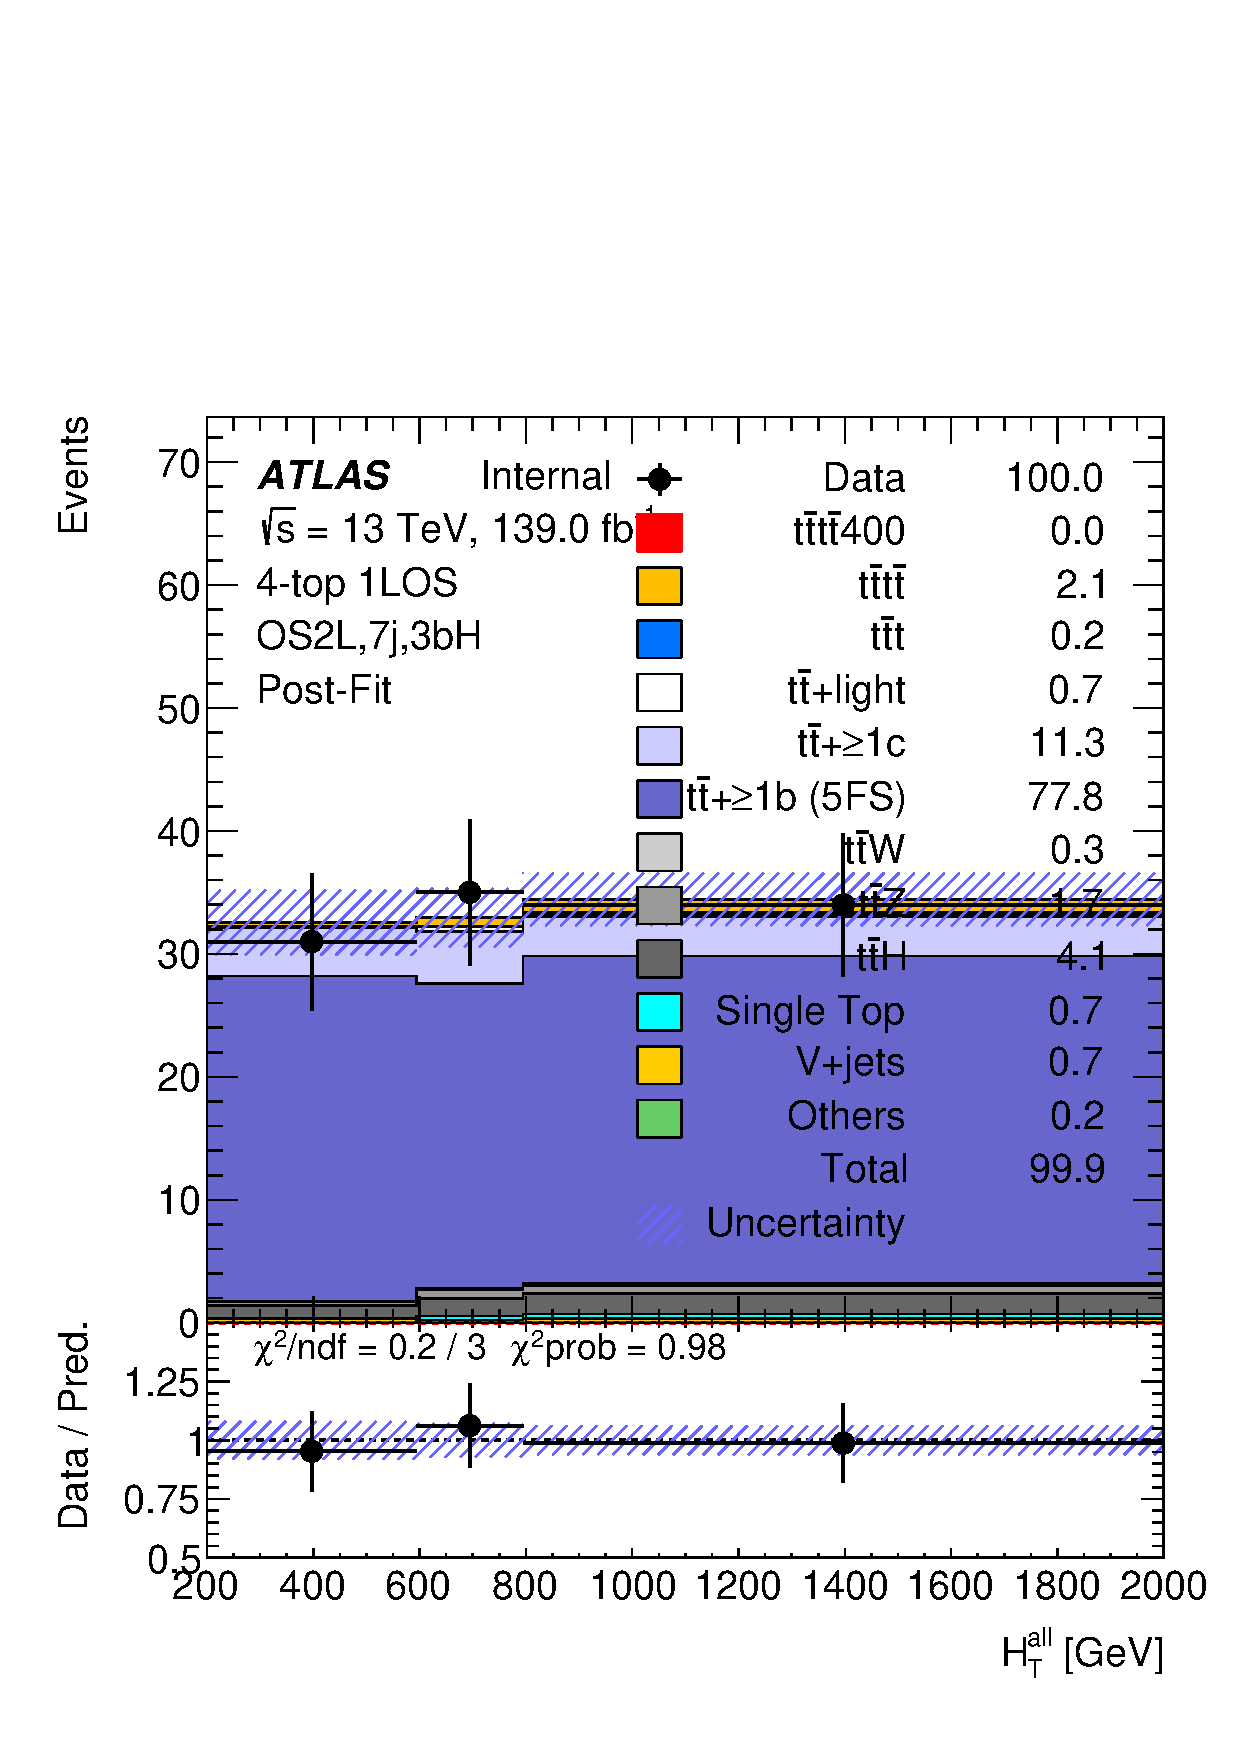
\includegraphics[width=0.31 \textwidth]{figures/fits/GNN/400/all/data_unblindedBonly/Plots/os2l_7j3bH_postFit.pdf} &
        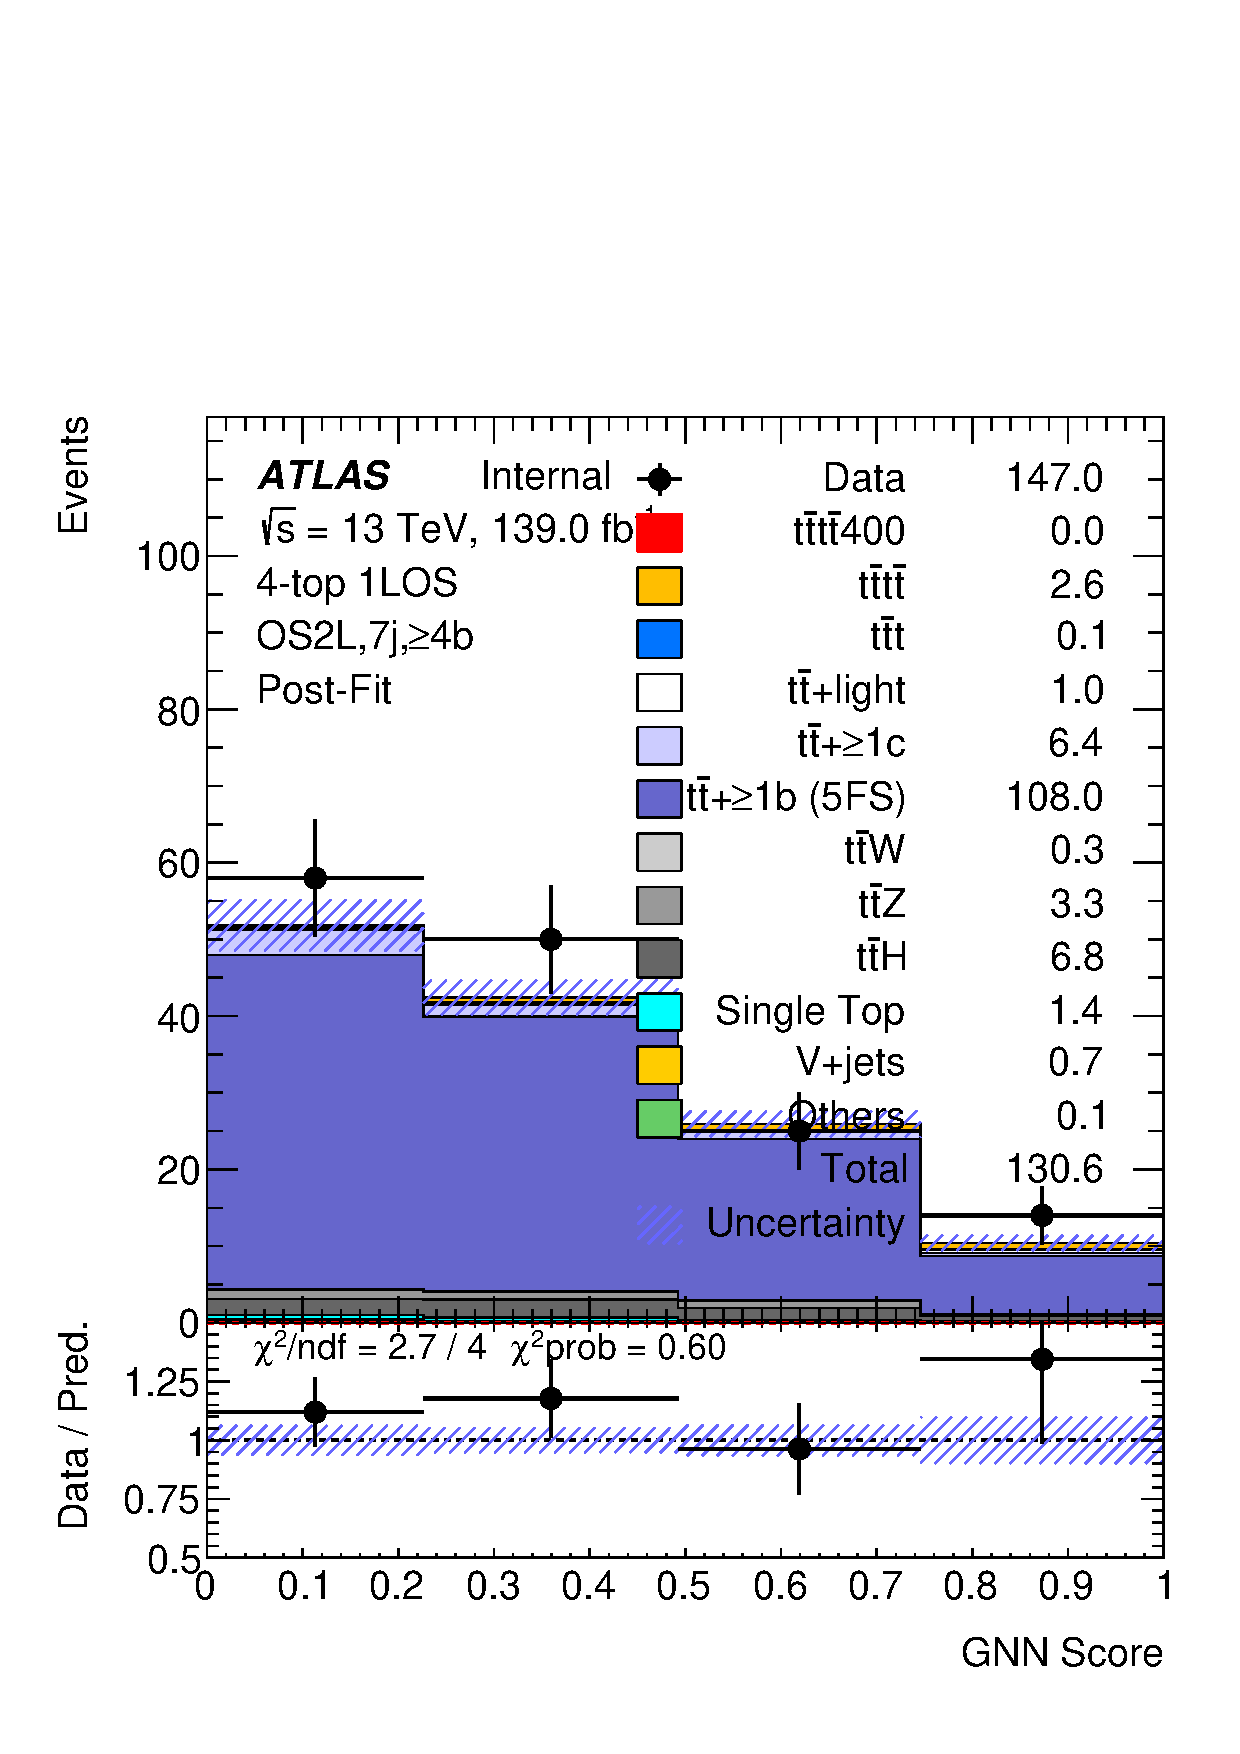
\includegraphics[width=0.31 \textwidth]{figures/fits/GNN/400/all/data_unblindedBonly/Plots/os2l_7jge4b_postFit.pdf} \\

        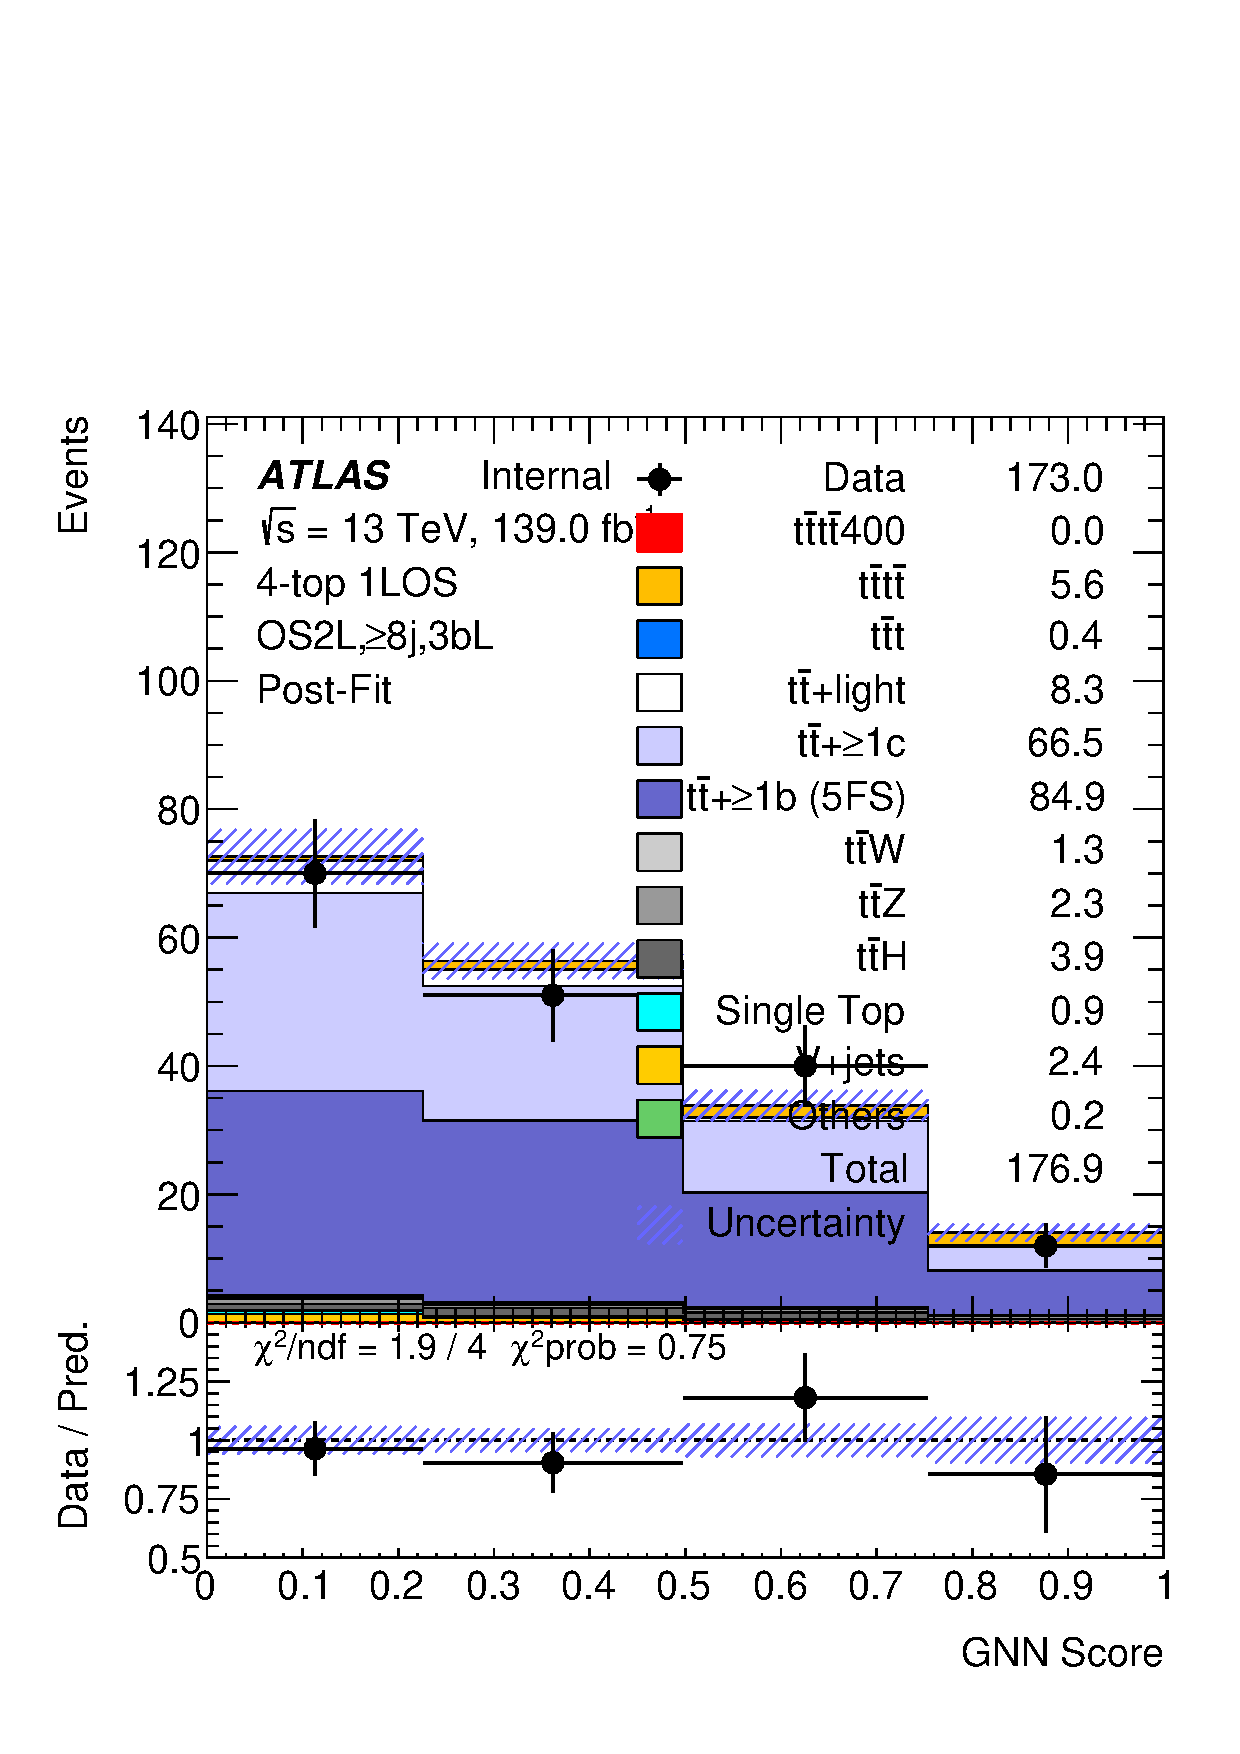
\includegraphics[width=0.31 \textwidth]{figures/fits/GNN/400/all/data_unblindedBonly/Plots/os2l_ge8j3bL_postFit.pdf} &
        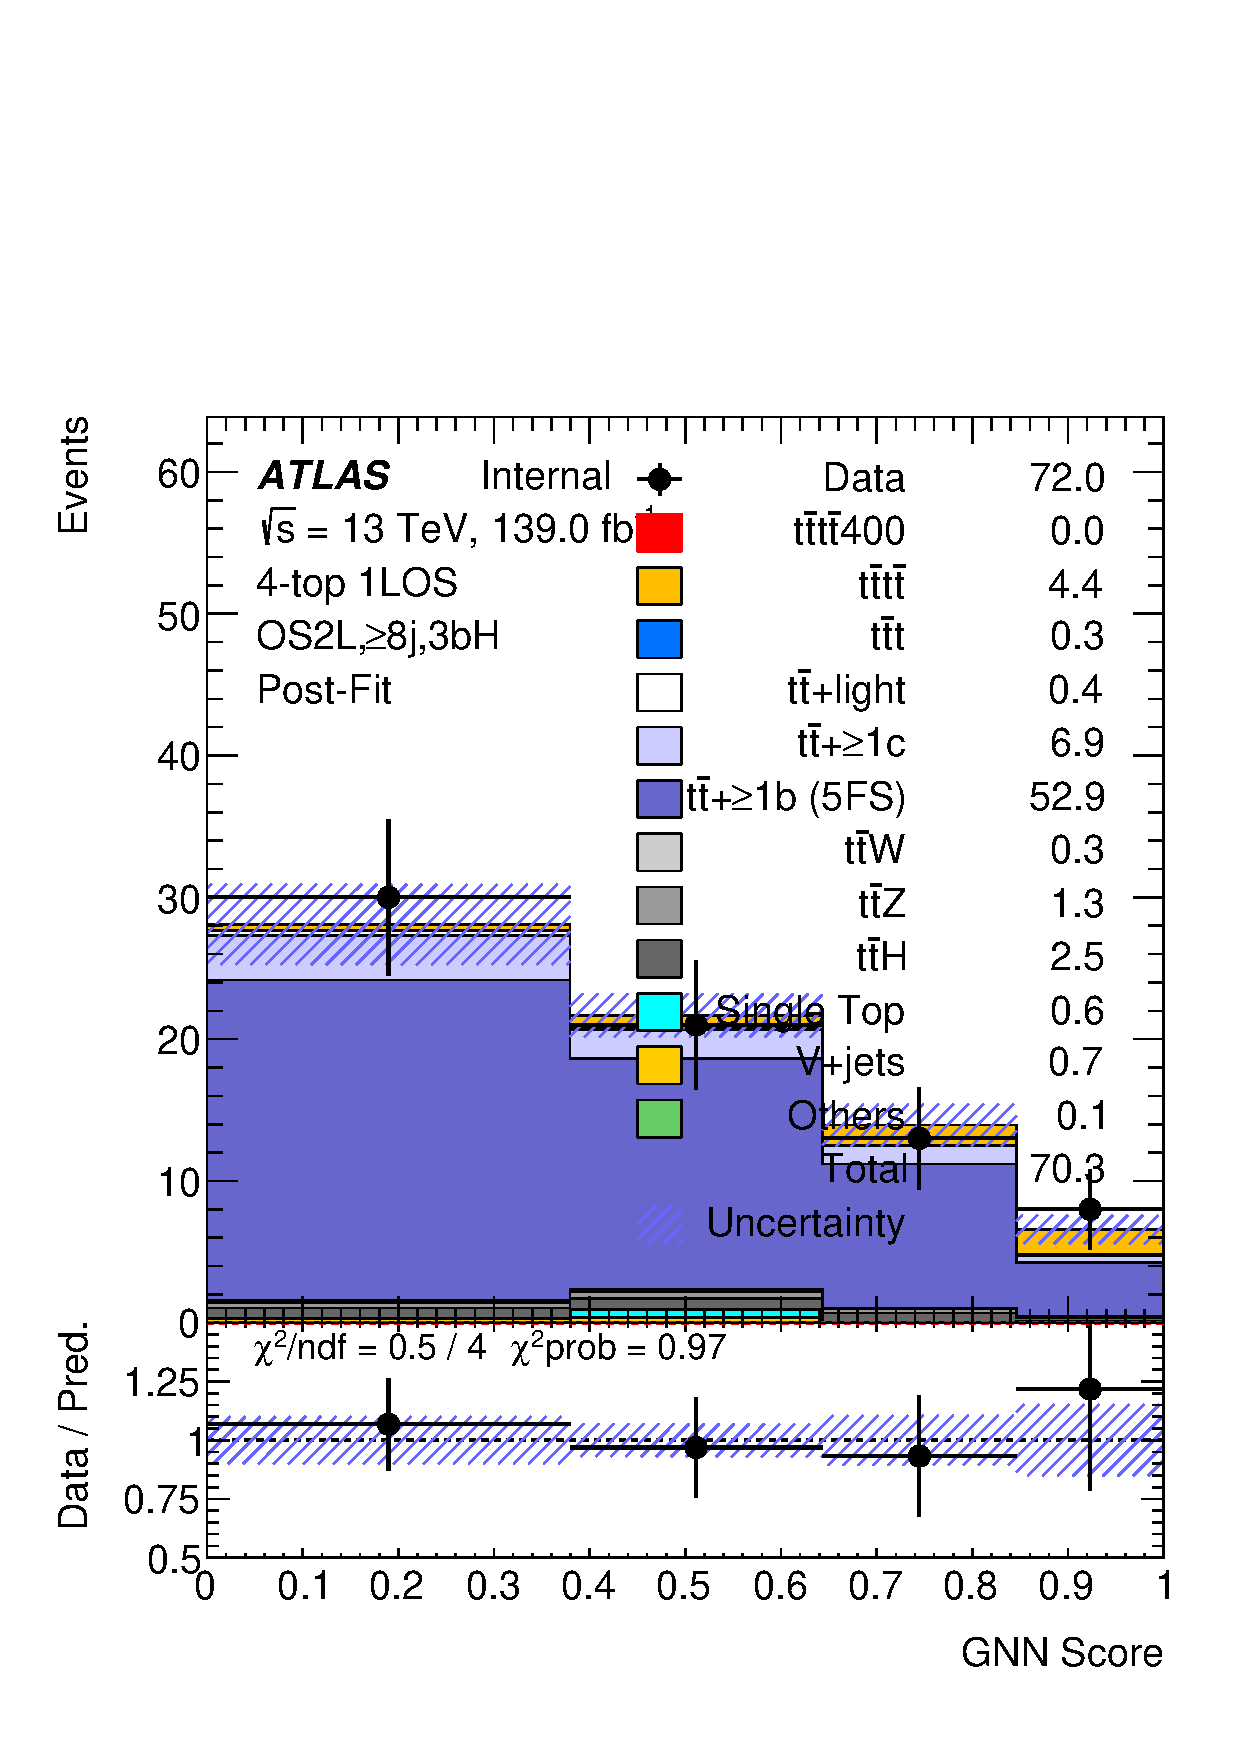
\includegraphics[width=0.31 \textwidth]{figures/fits/GNN/400/all/data_unblindedBonly/Plots/os2l_ge8j3bH_postFit.pdf} &
        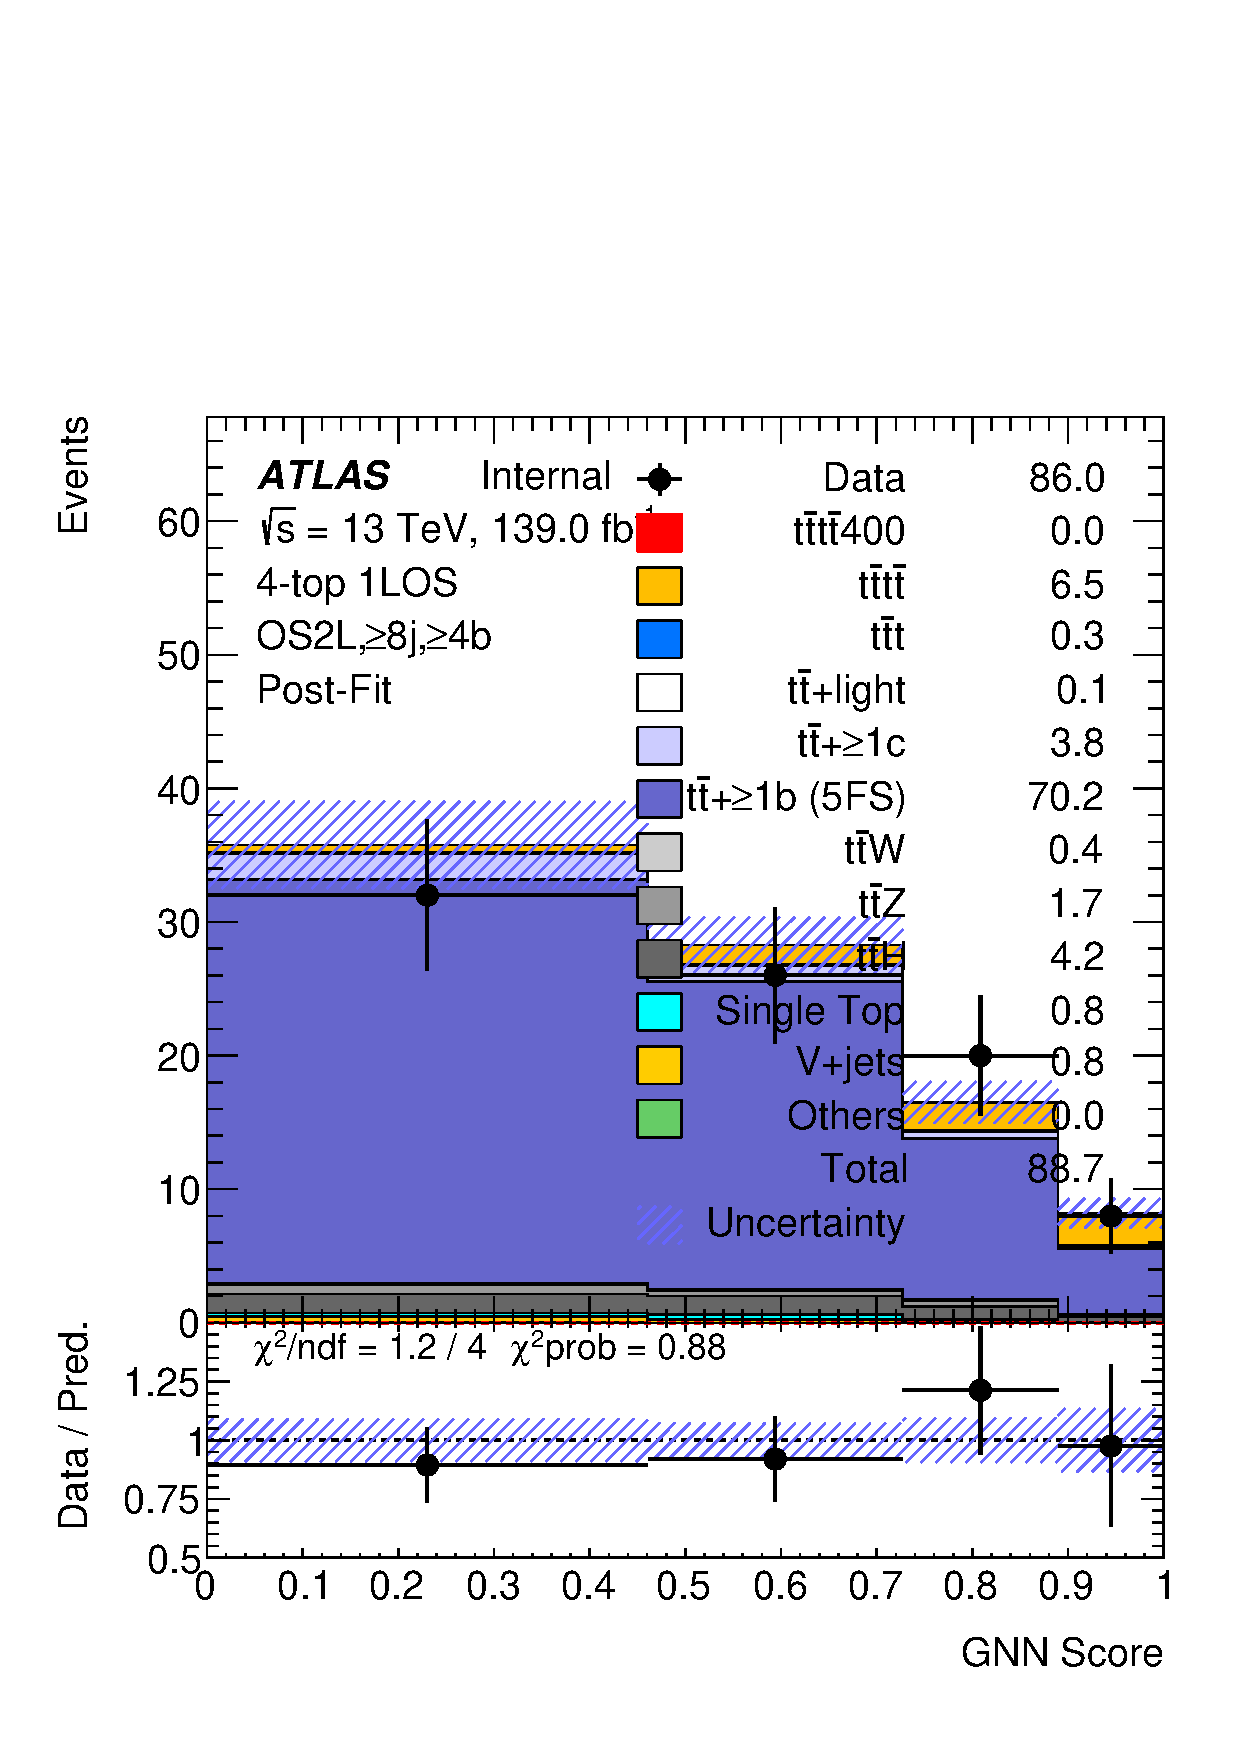
\includegraphics[width=0.31 \textwidth]{figures/fits/GNN/400/all/data_unblindedBonly/Plots/os2l_ge8jge4b_postFit.pdf} \\
        \end{tabular}
        \caption{\label{fig:unblinded_data_Bonly_postfit_2L}
        Post-fit distributions for the 2LOS regions obtained from the background-only unblinded data fit at $\boldsymbol{m_H=400}$~GeV. 
        The fit is performed using all regions (1L+2LOS).}
\end{center}
\end{figure}

\subsubsection*{\textbf{Nuisance parameters and correlations}}

The fitted pulls and constraints of nuisance parameters in the combined (1L+2LOS) background-only fit are compared across several mass hypotheses in Figure~\ref{fig:unblinded_data_Bonly_NP_mass_all}. 
Only the simultaneous fit to all regions (1L+2LOS) is shown, since this configuration is used for the extraction of physics results. 
The behaviour of the nuisance parameters is stable across the tested mass points, with no large pulls or over-constrained parameters observed.

\begin{figure}[htbp!]
  \centering
  \begin{subfigure}[t]{0.32\textwidth}
    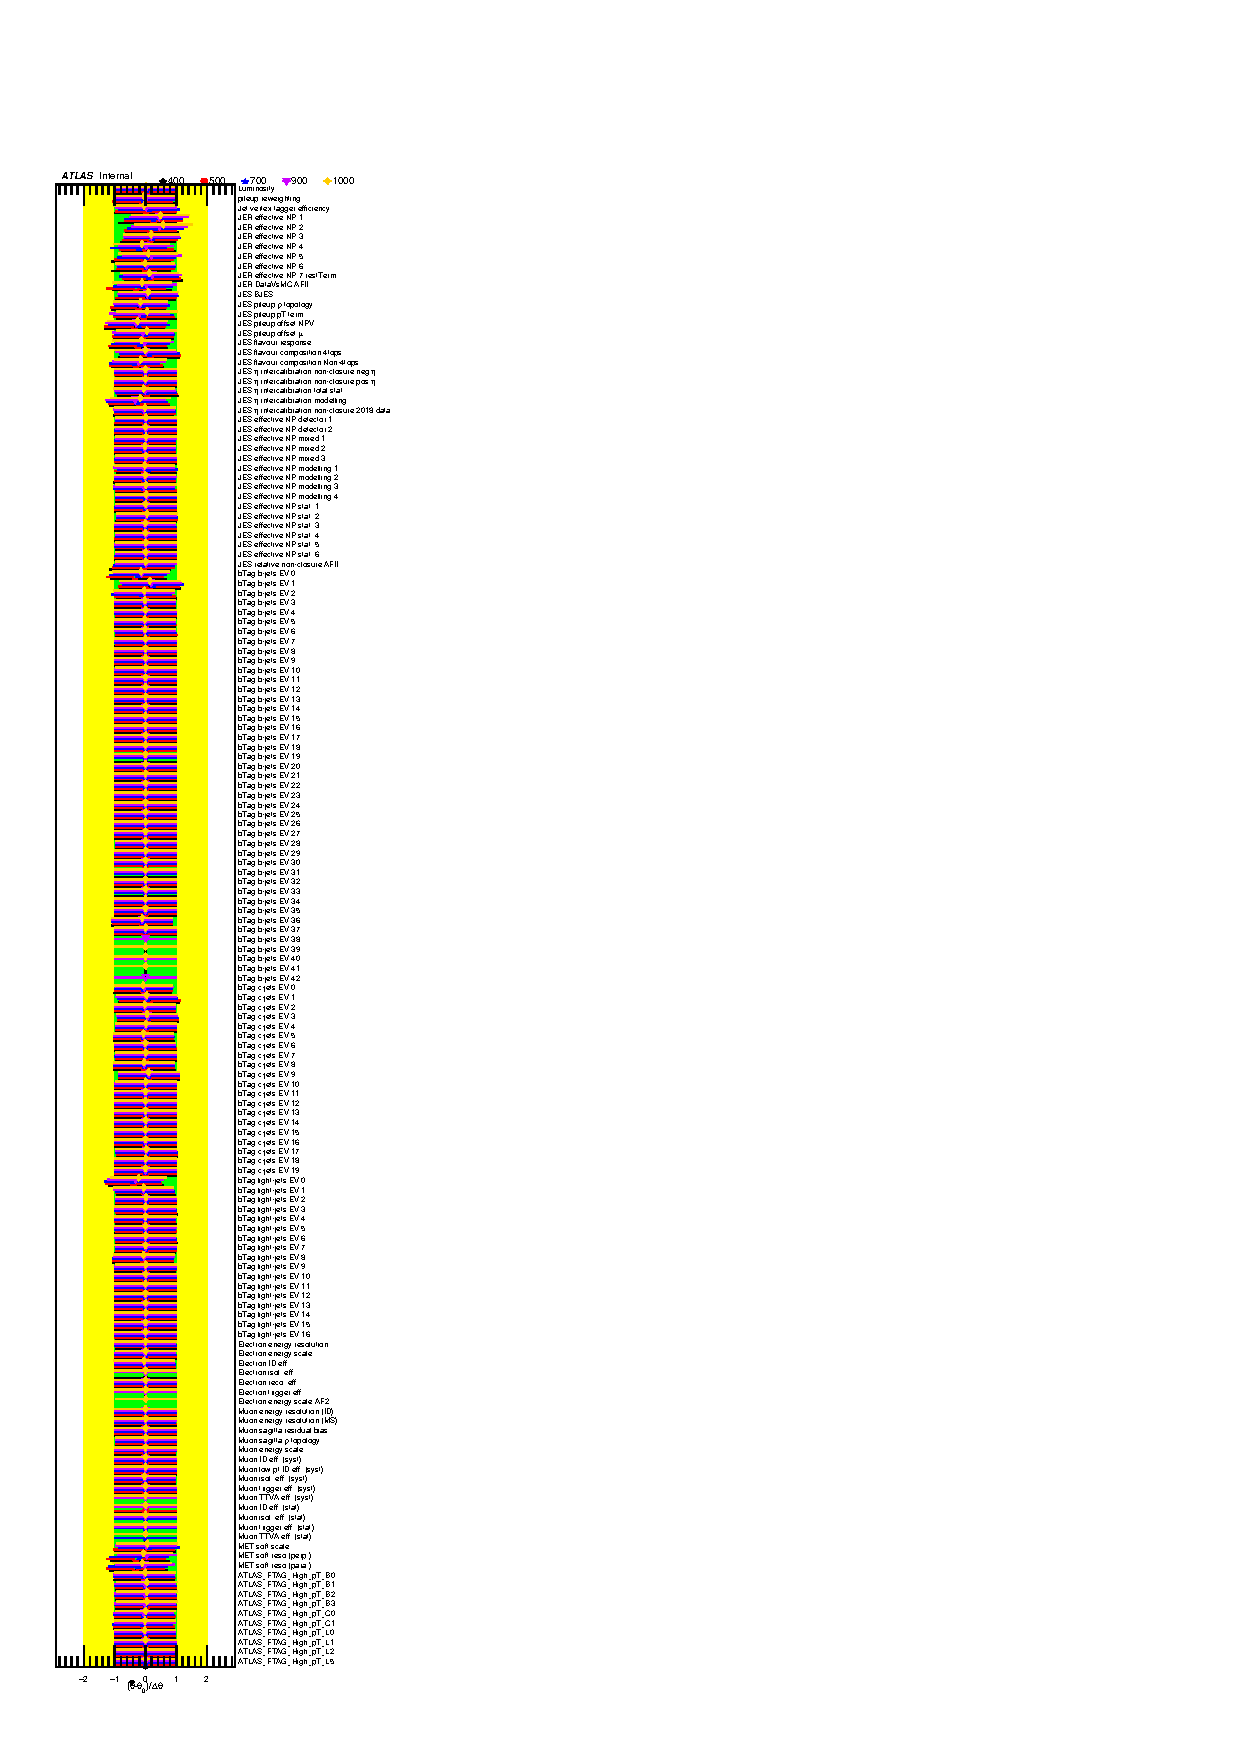
\includegraphics[width=\linewidth]{figures/fits/comparisons/massPoints/GNN/all/data_unblindedBonly/NuisPar_comp_Instrumental.pdf}
    \subcaption{Instrumental}
    \label{fig:unblinded_data_Bonly_NP_mass_all_instrumental}
  \end{subfigure}
  \begin{subfigure}[t]{0.32\textwidth}
    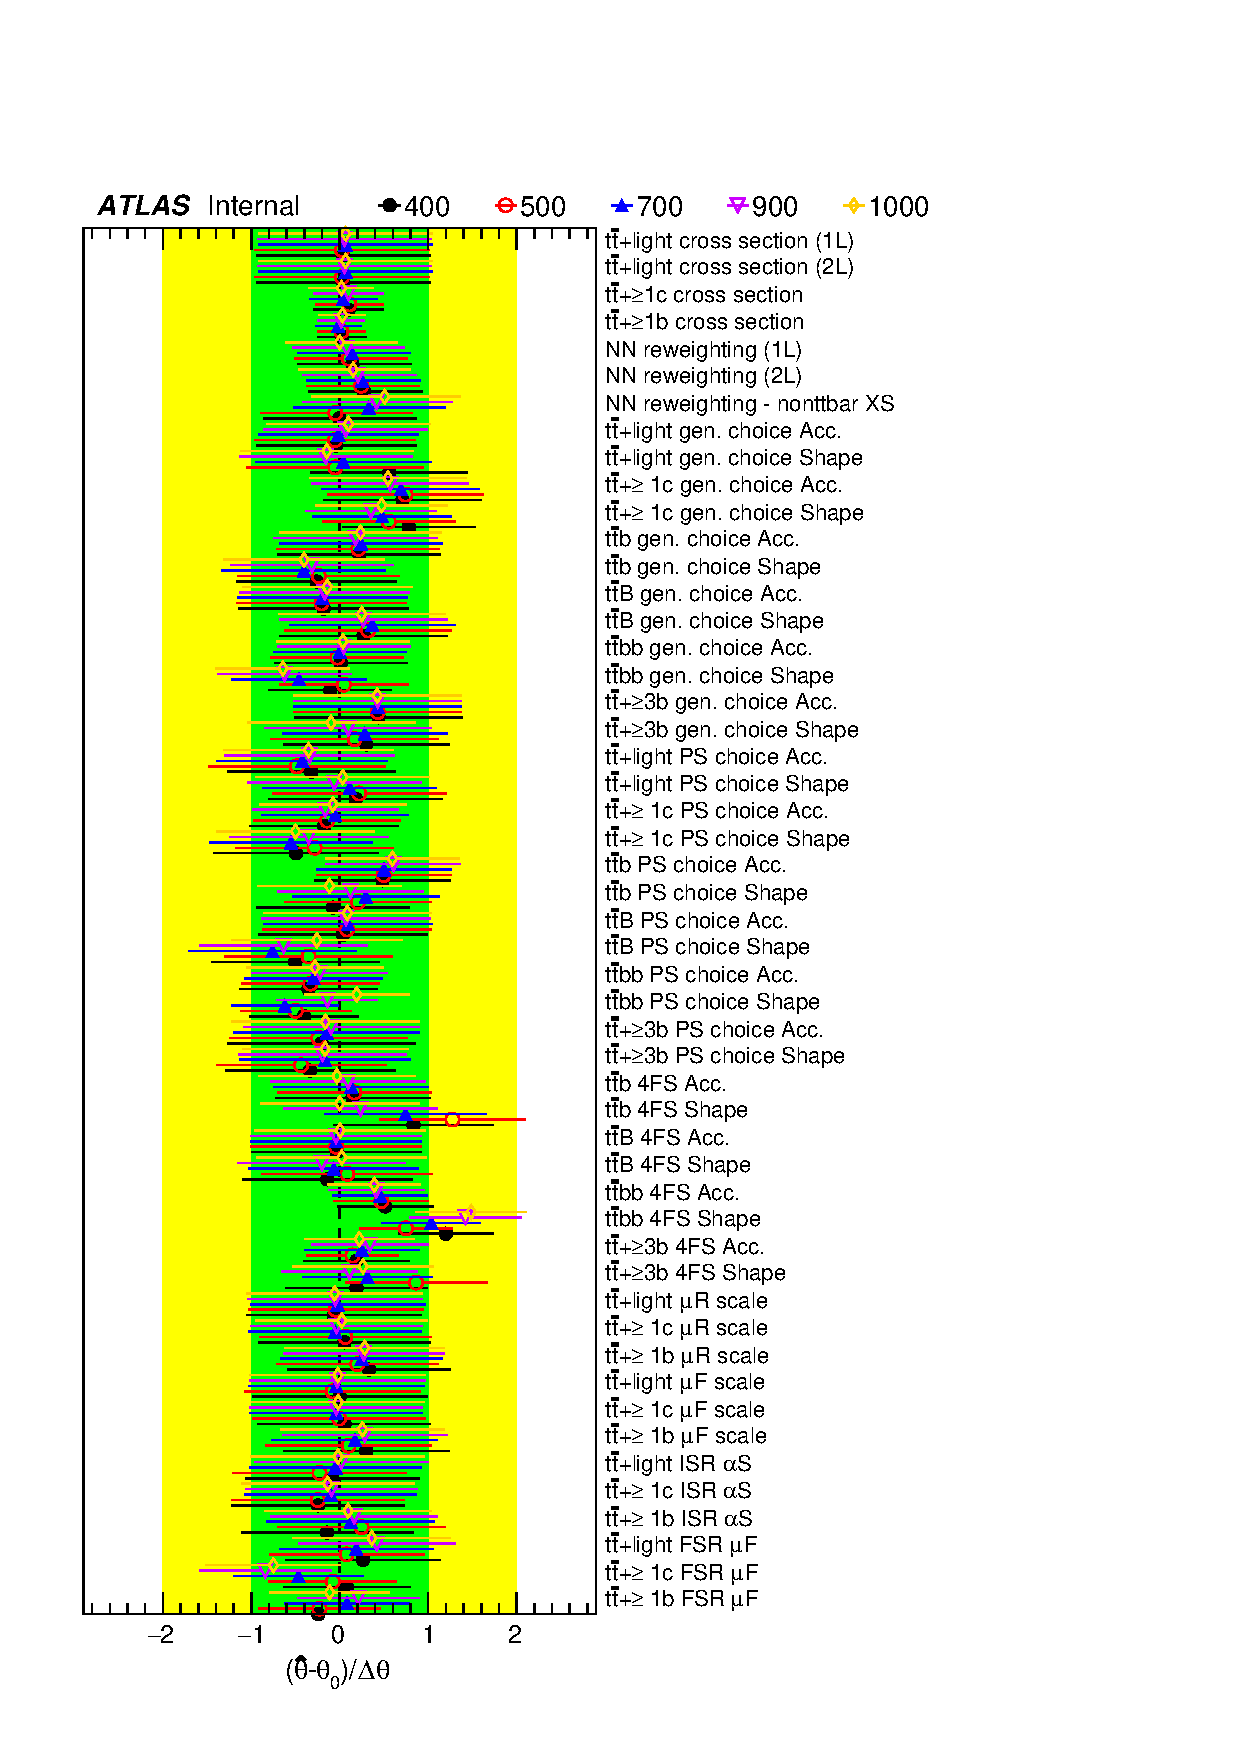
\includegraphics[width=\linewidth]{figures/fits/comparisons/massPoints/GNN/all/data_unblindedBonly/NuisPar_comp_ttbar.pdf}
    \subcaption{$\boldsymbol{t\bar{t}}$ modelling}
    \label{fig:unblinded_data_Bonly_NP_mass_all_ttbar}
  \end{subfigure}
  \begin{subfigure}[t]{0.32\textwidth}
    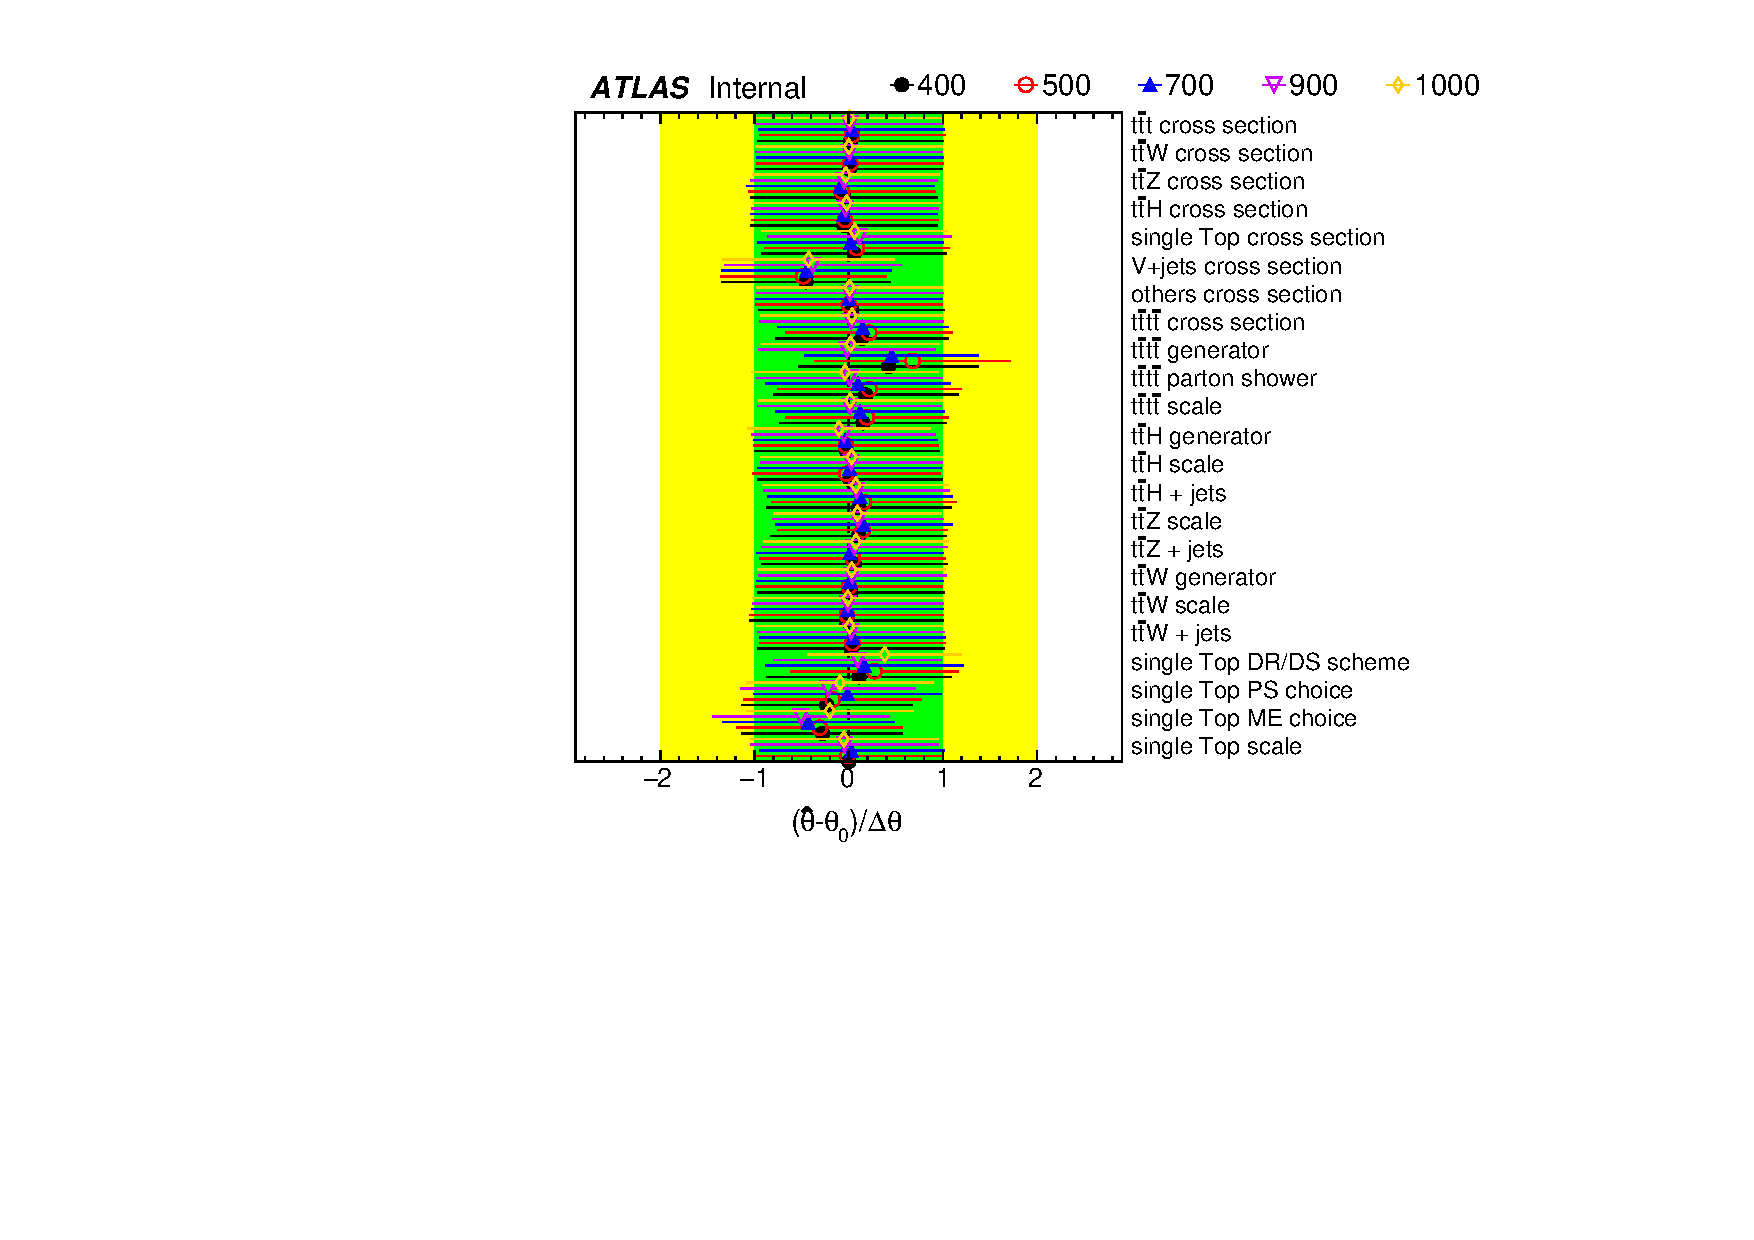
\includegraphics[width=\linewidth]{figures/fits/comparisons/massPoints/GNN/all/data_unblindedBonly/NuisPar_comp_Other.pdf}
    \subcaption{Other backgrounds}
    \label{fig:unblinded_data_Bonly_NP_mass_all_other}
  \end{subfigure}
  \caption{\label{fig:unblinded_data_Bonly_NP_mass_all}
  Fitted pulls and constraints for nuisance parameters in the combined (1L+2LOS) background-only unblinded data fit, shown for several mass hypotheses.}
\end{figure}

The correlation matrix of the combined background-only fit at $m_H=400$~GeV is shown in Figure~\ref{fig:unblinded_data_Bonly_corr_mH400_Data_all}. 
The observed correlations follow the expected structure, with moderate correlations among related background normalisation parameters.

\begin{figure}[htbp!]
  \centering
  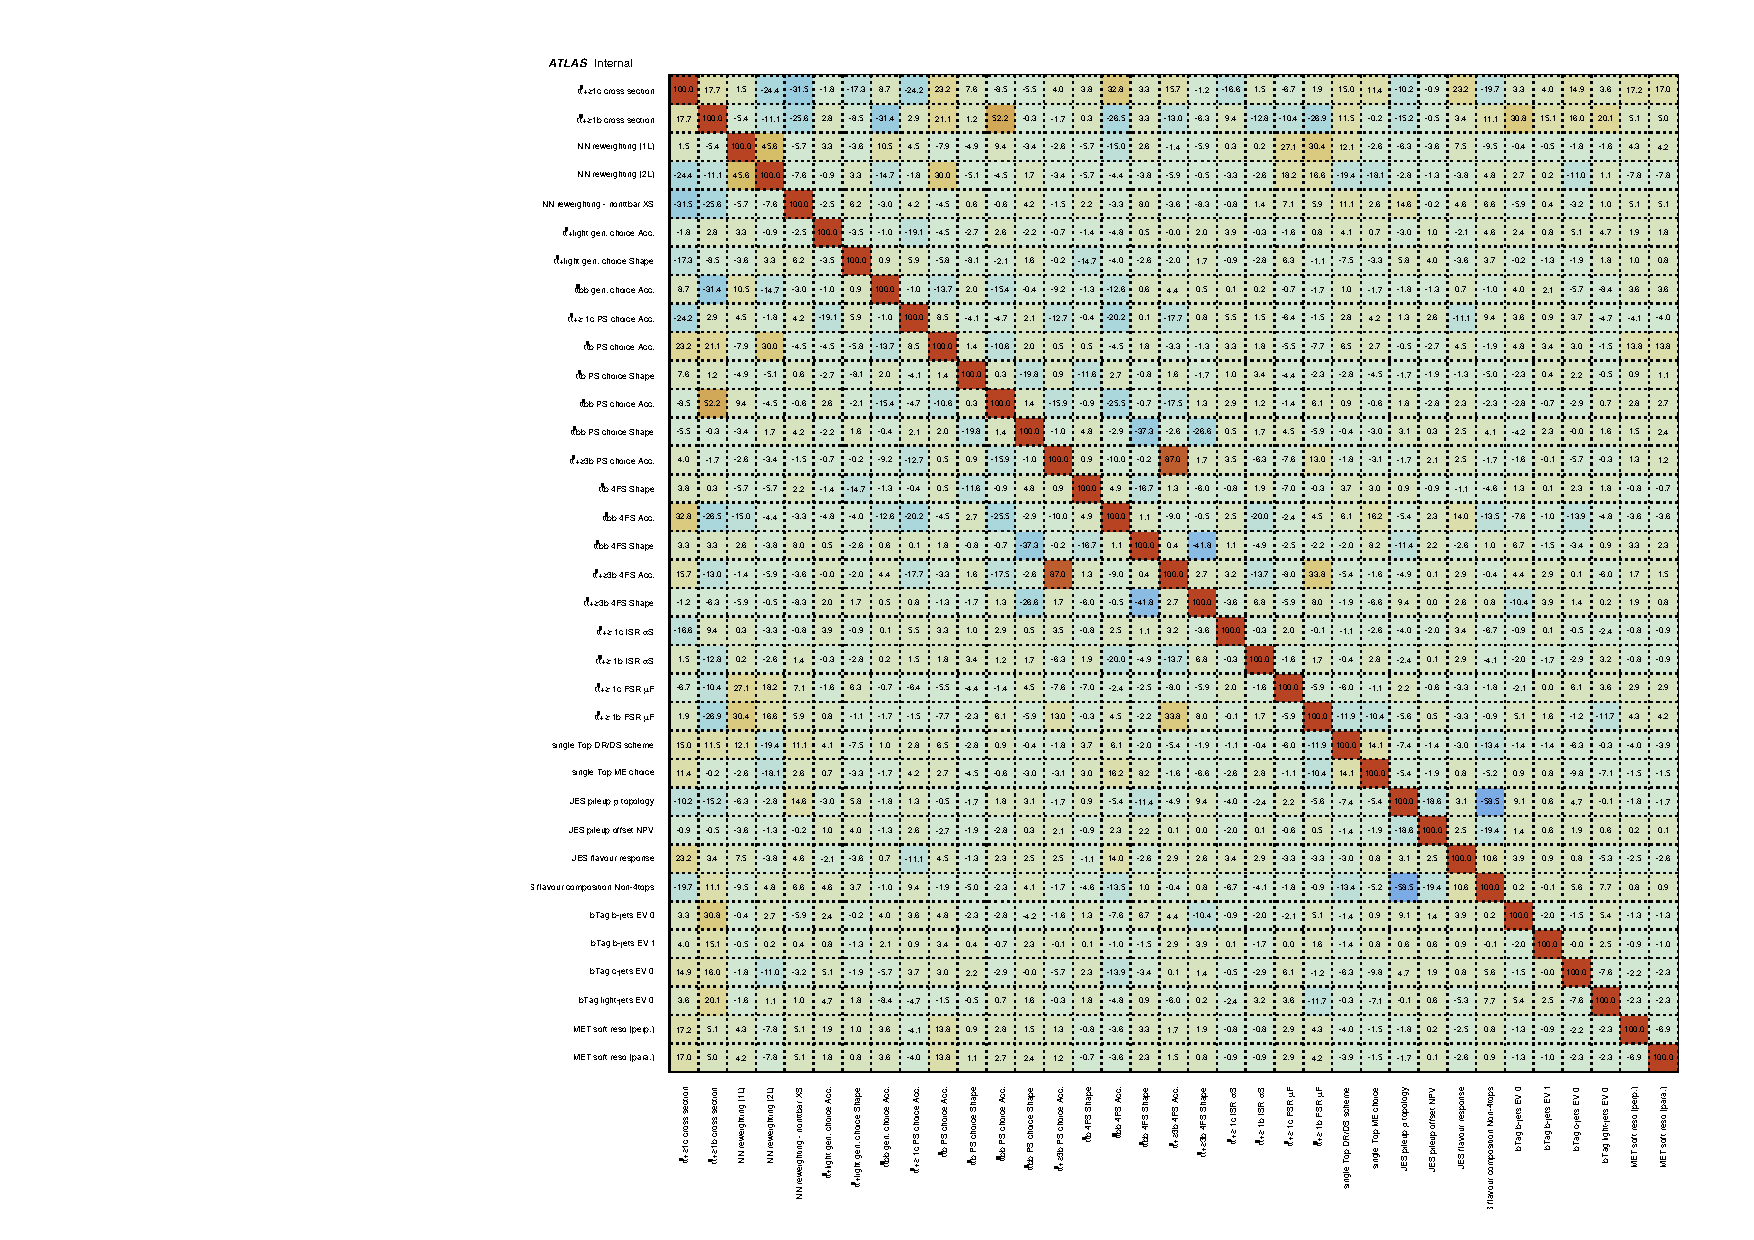
\includegraphics[width=\linewidth]{figures/fits/GNN/400/all/data_unblindedBonly/CorrMatrix.pdf}
  \caption{\label{fig:unblinded_data_Bonly_corr_mH400_Data_all}
  Correlation matrix of nuisance parameters in the combined background-only unblinded data fit for $\boldsymbol{m_H=400}$~GeV.}
\end{figure}

Overall, the background-only fit demonstrates stable behaviour and good agreement with the observed data. 
The validated background model provides a reliable basis for the subsequent signal-plus-background fit and limit extraction.

\subsection{Signal-plus-background fit results}
\label{sec:splusb_fit}

In contrast to the background-only fit, a signal-plus-background (S+B) fit is performed by allowing the signal strength parameter $\mu$ to float freely in the likelihood.
The fit is carried out simultaneously across all control and signal regions in the combined 1L and 2LOS channels, with all systematic uncertainties profiled. 
% The dominant $t\bar{t}$ background is corrected using the neural-network-based reweighting described in Section~XX.

\subsubsection*{\textbf{Post-fit agreement}}

The post-fit distributions for a representative mass point of $m_H=400$~GeV are shown in Figures~\ref{fig:unblinded_data_SplusB_postfit_1L} and~\ref{fig:unblinded_data_SplusB_postfit_2L} for the 1L and 2LOS regions, respectively. 
The fit is performed using all regions (1L+2LOS). 
Good agreement between data and the post-fit prediction is observed across all regions. 
No statistically significant excess is observed.

\begin{figure}[htbp!]
        \begin{center} \setlength{\tabcolsep}{2.5pt}\footnotesize
        \begin{tabular}{cccc}
        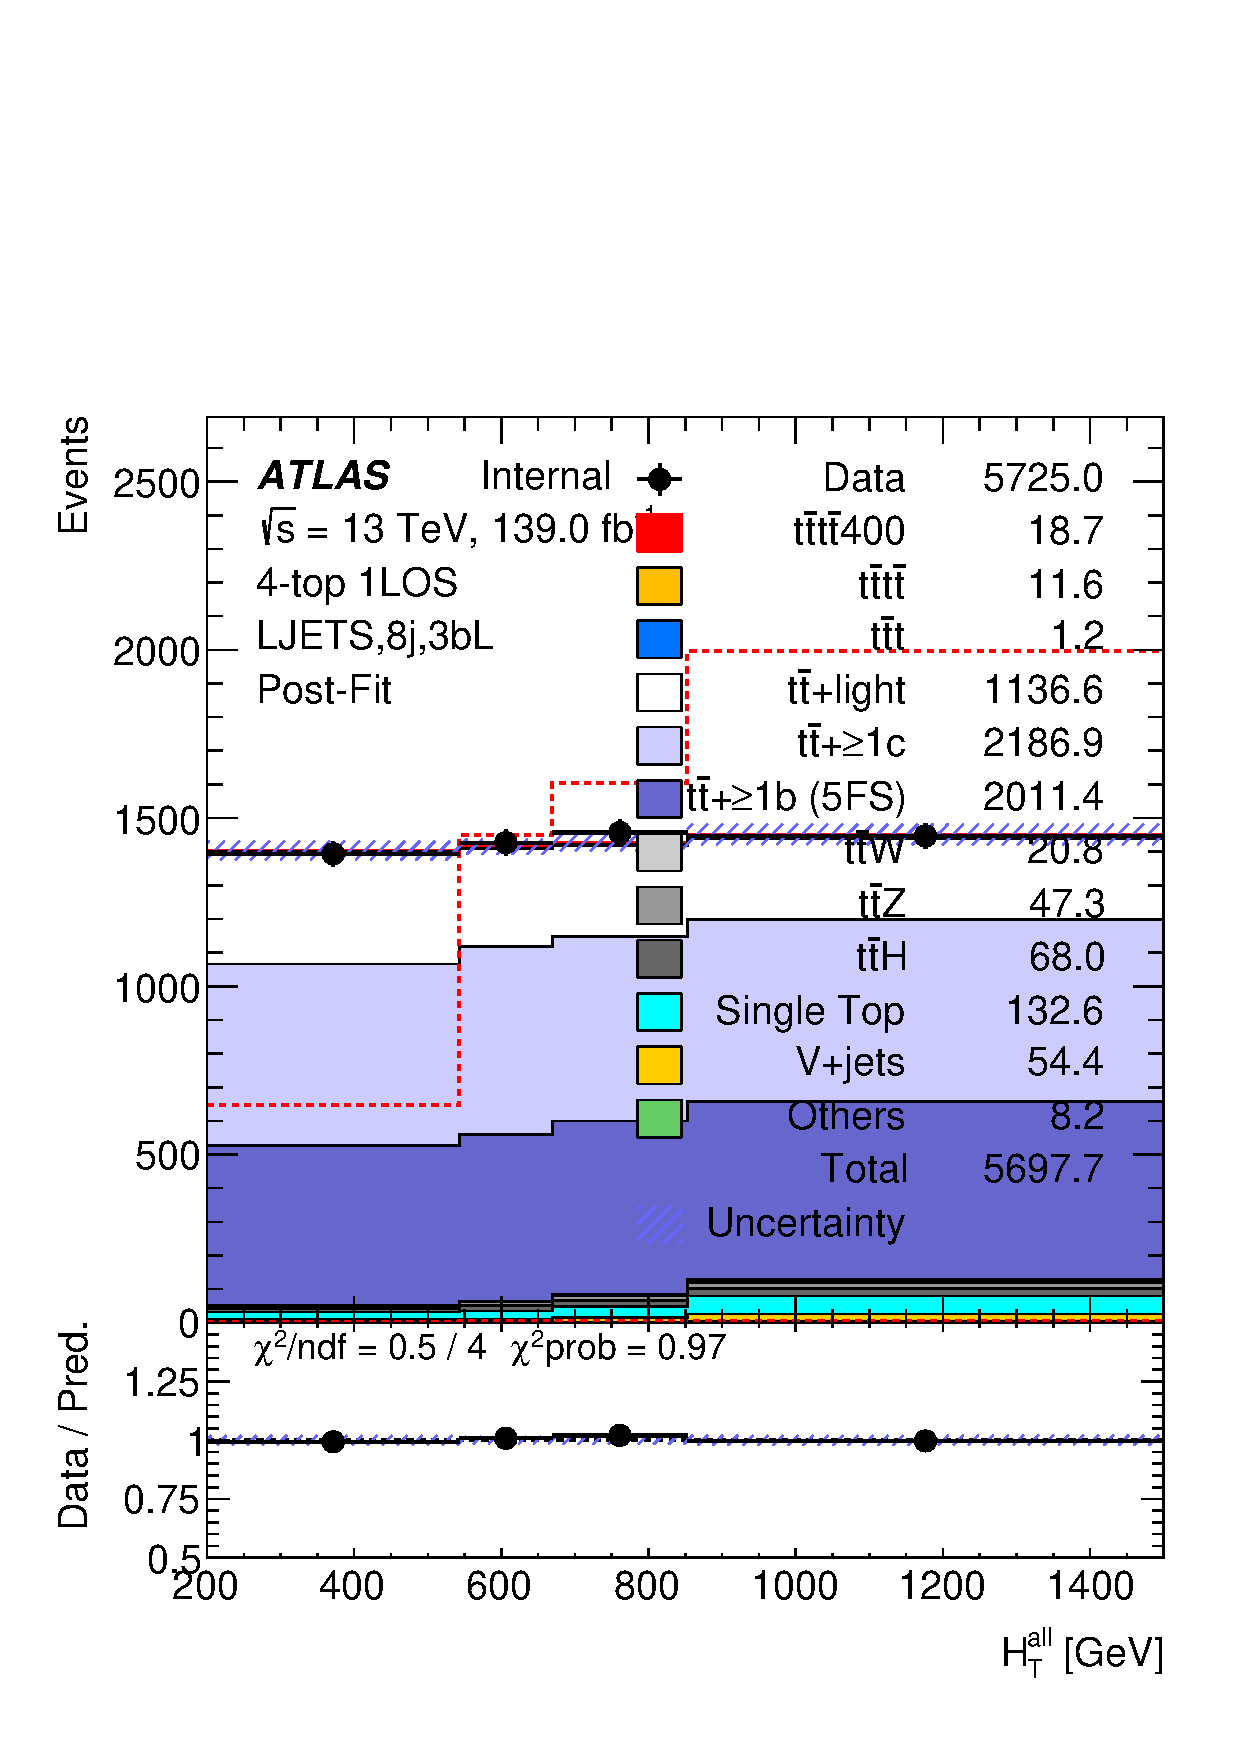
\includegraphics[width=0.23 \textwidth]{figures/fits/GNN/400/all/data_unblindedSplusB/Plots/ljets_8j3bL_postFit.pdf} &
        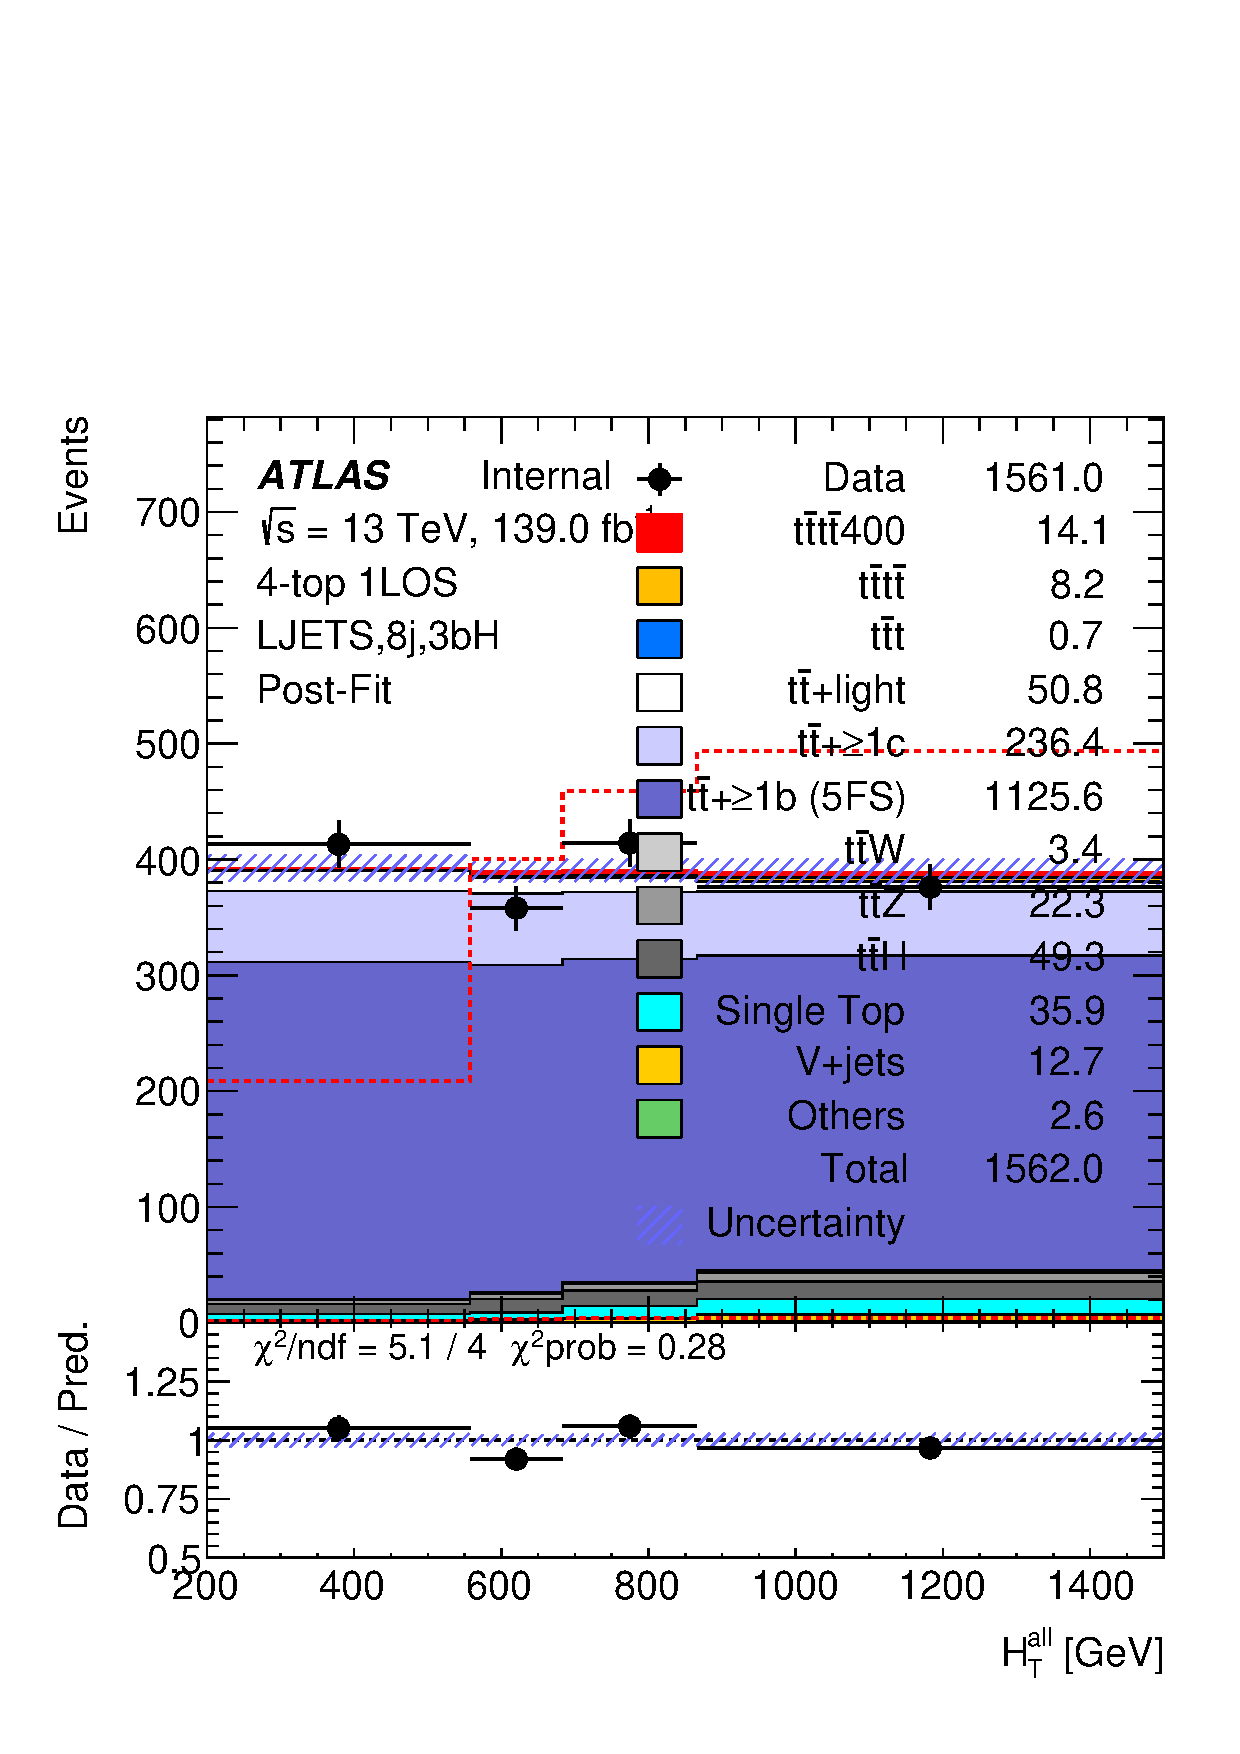
\includegraphics[width=0.23 \textwidth]{figures/fits/GNN/400/all/data_unblindedSplusB/Plots/ljets_8j3bH_postFit.pdf} &
        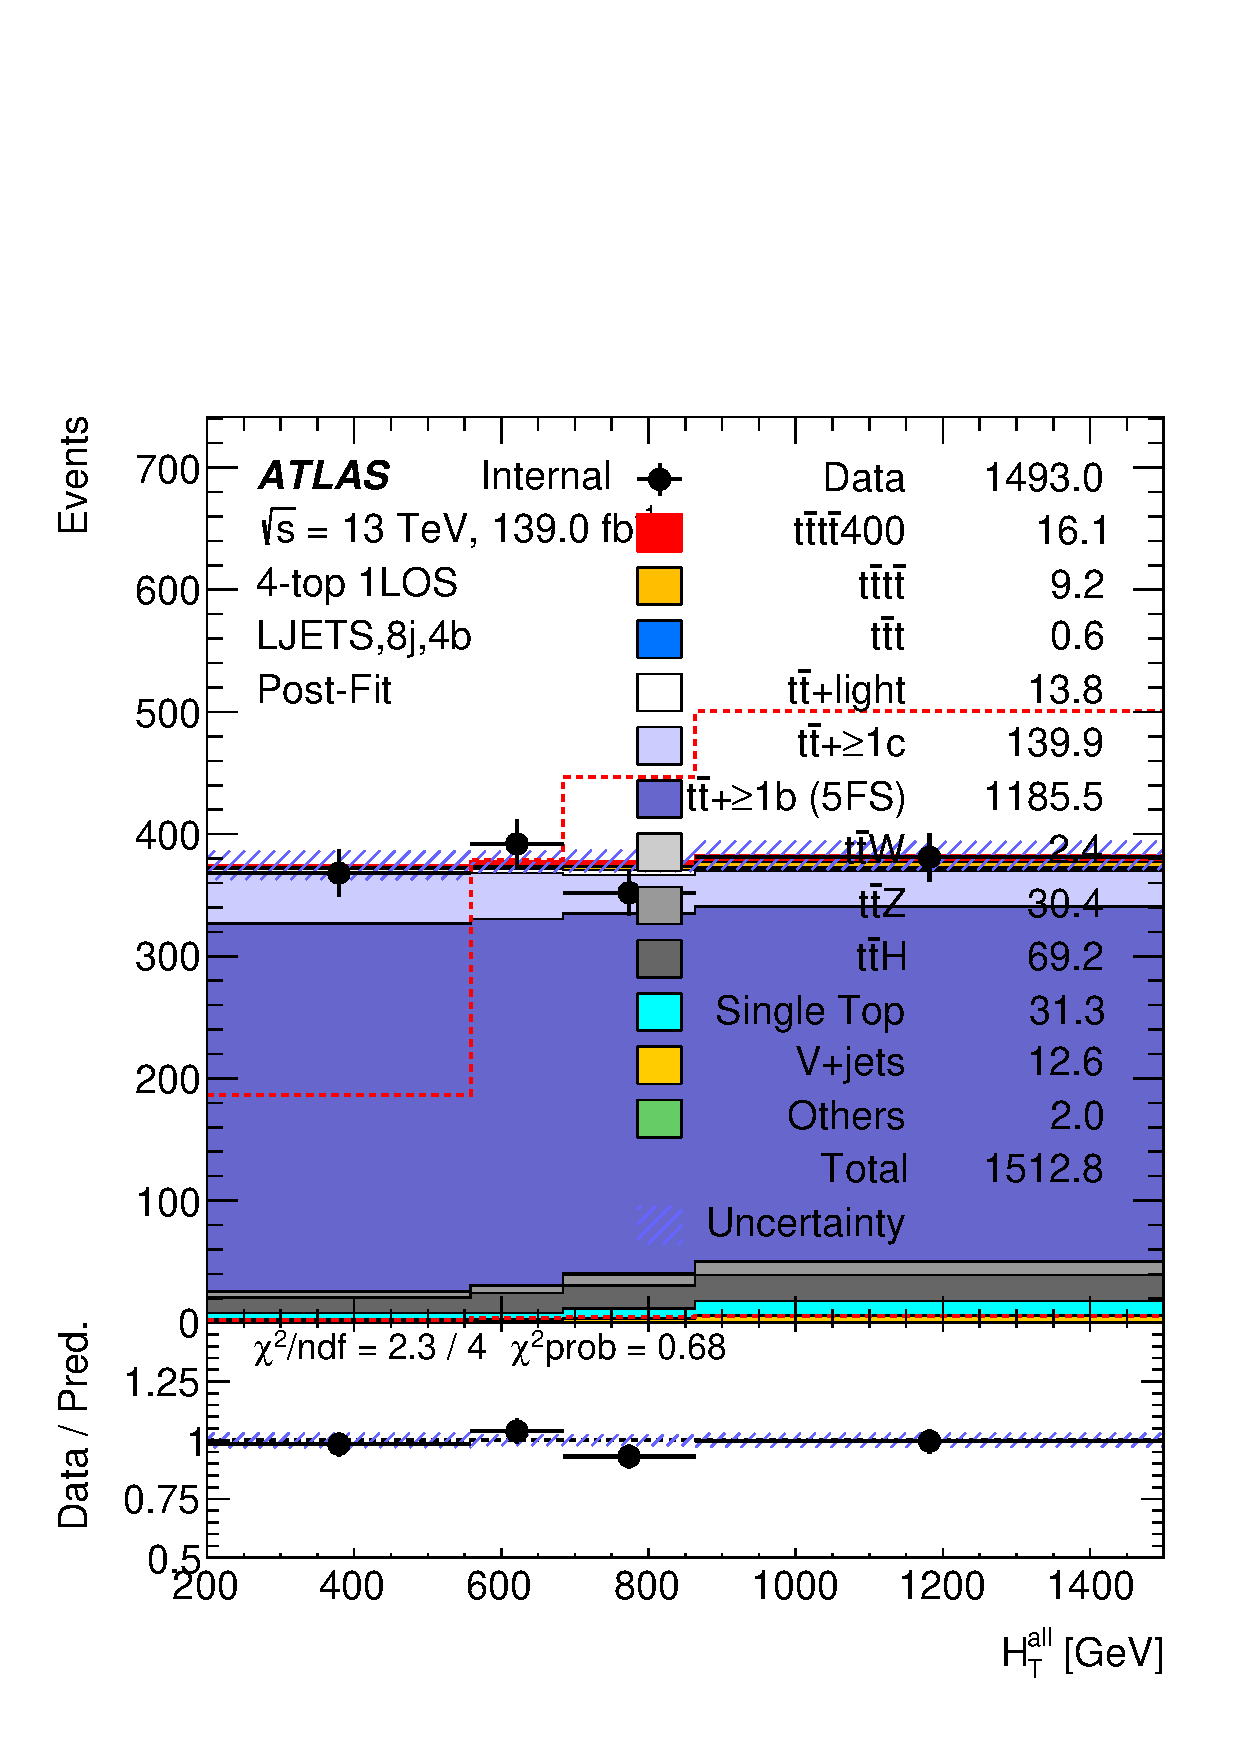
\includegraphics[width=0.23 \textwidth]{figures/fits/GNN/400/all/data_unblindedSplusB/Plots/ljets_8j4b_postFit.pdf} &
        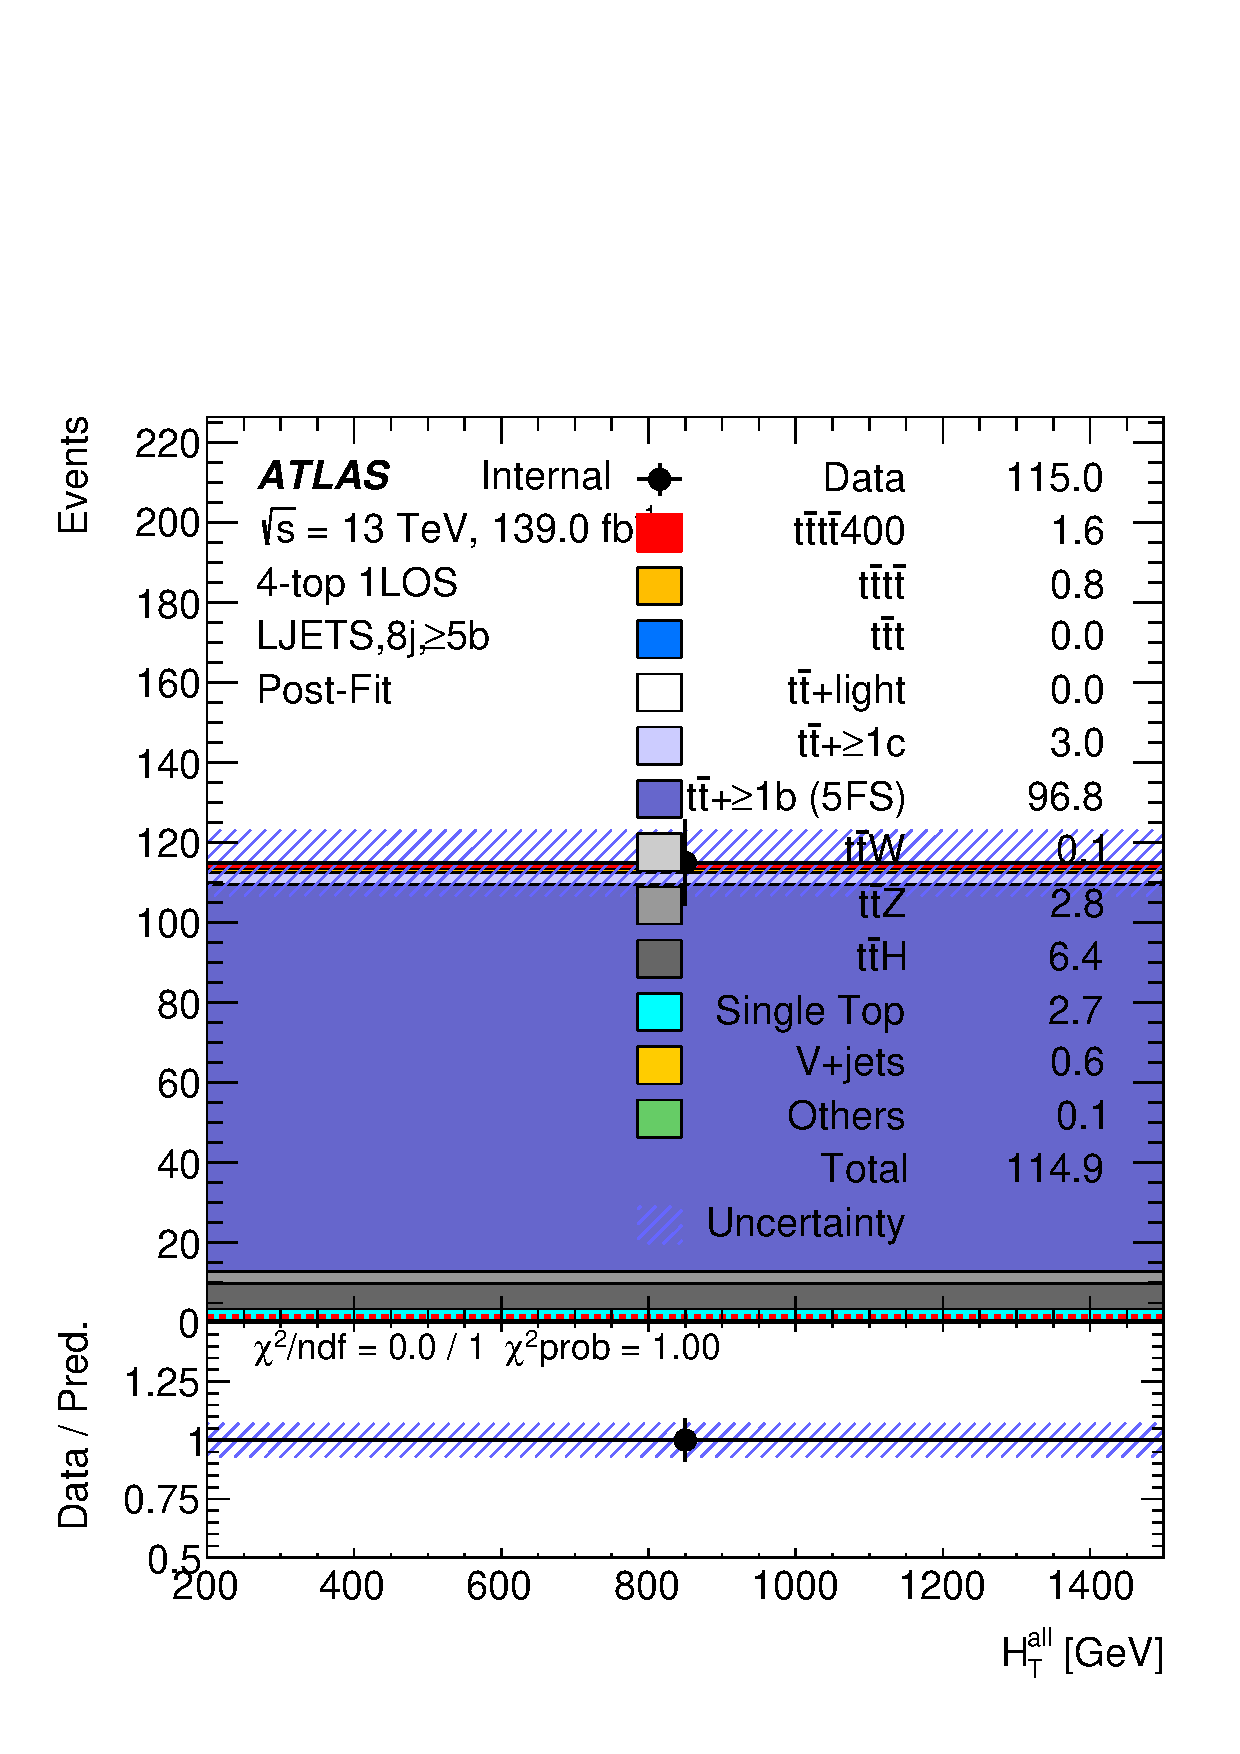
\includegraphics[width=0.23 \textwidth]{figures/fits/GNN/400/all/data_unblindedSplusB/Plots/ljets_8jge5b_postFit.pdf}\\

        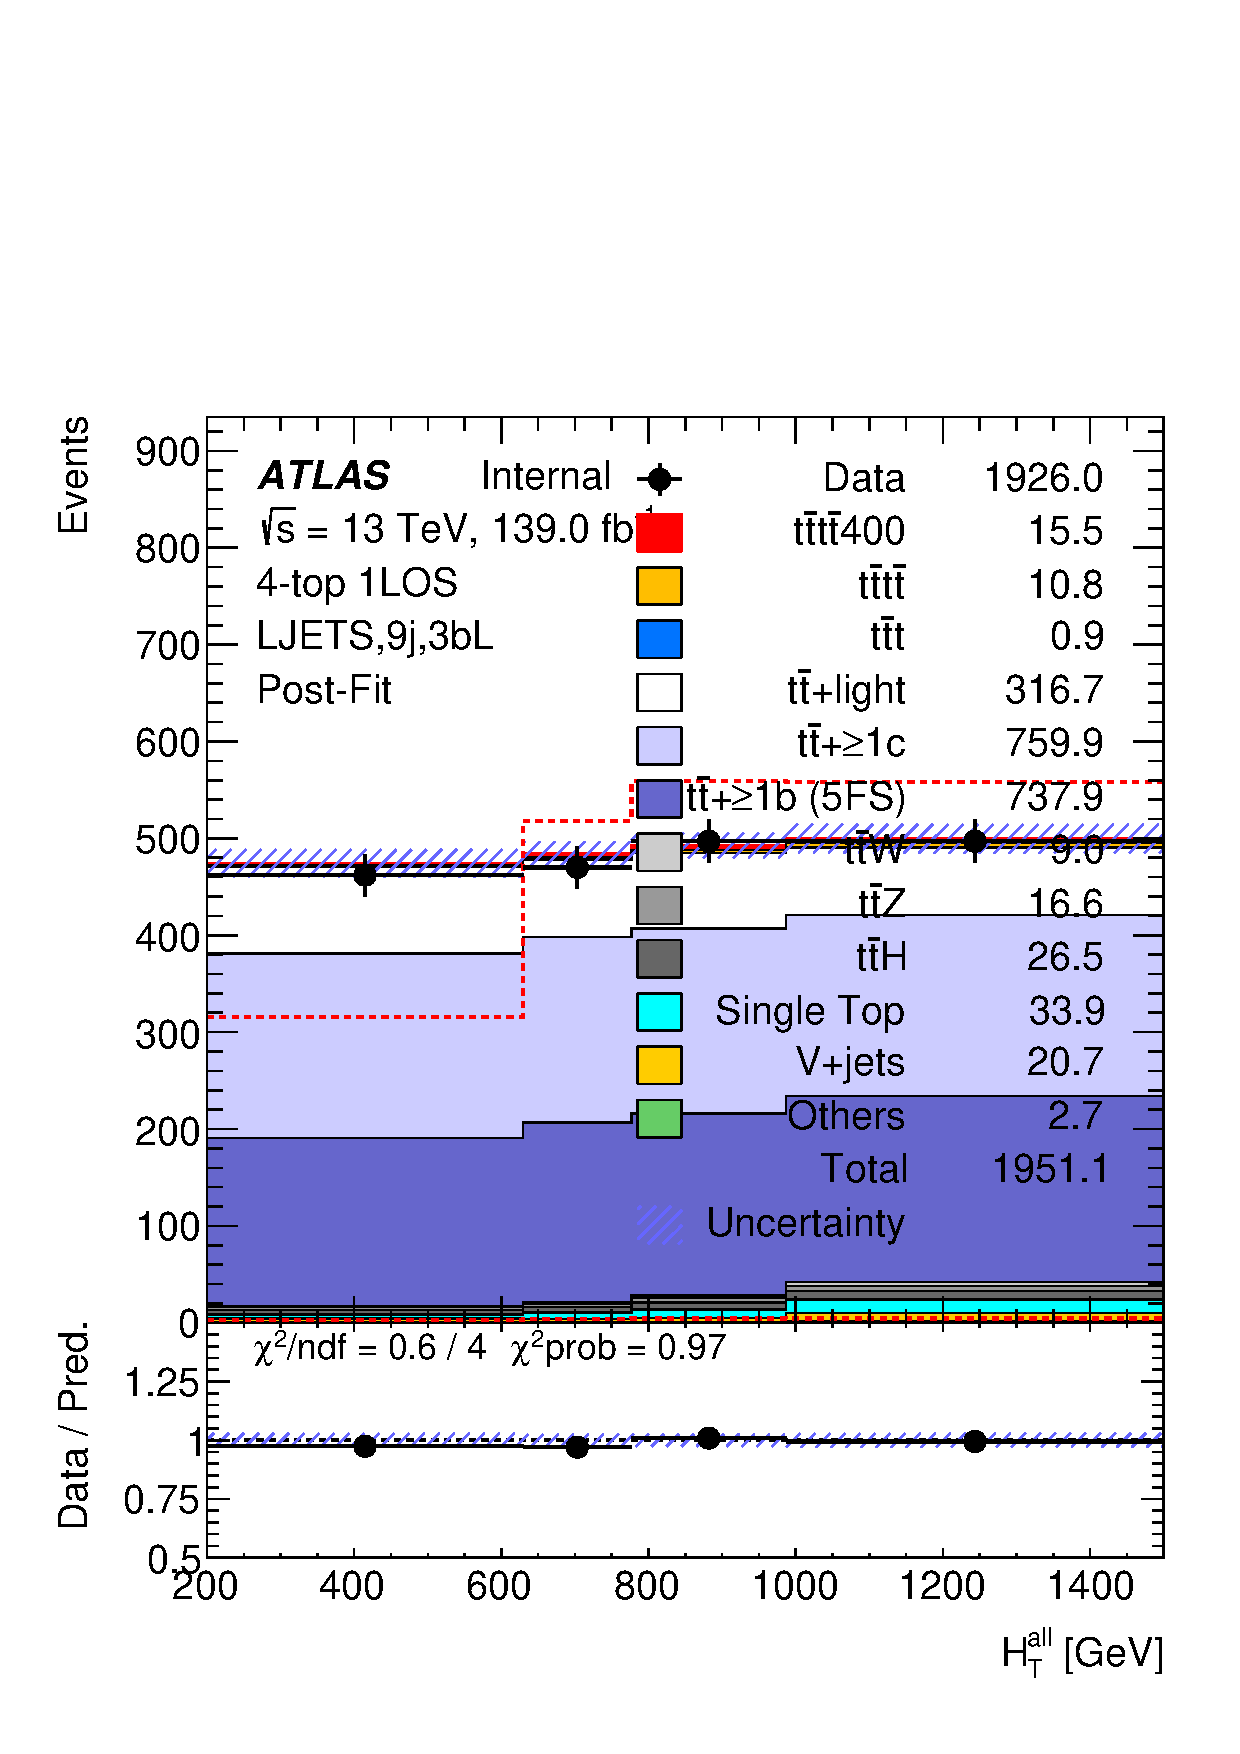
\includegraphics[width=0.23 \textwidth]{figures/fits/GNN/400/all/data_unblindedSplusB/Plots/ljets_9j3bL_postFit.pdf} &
        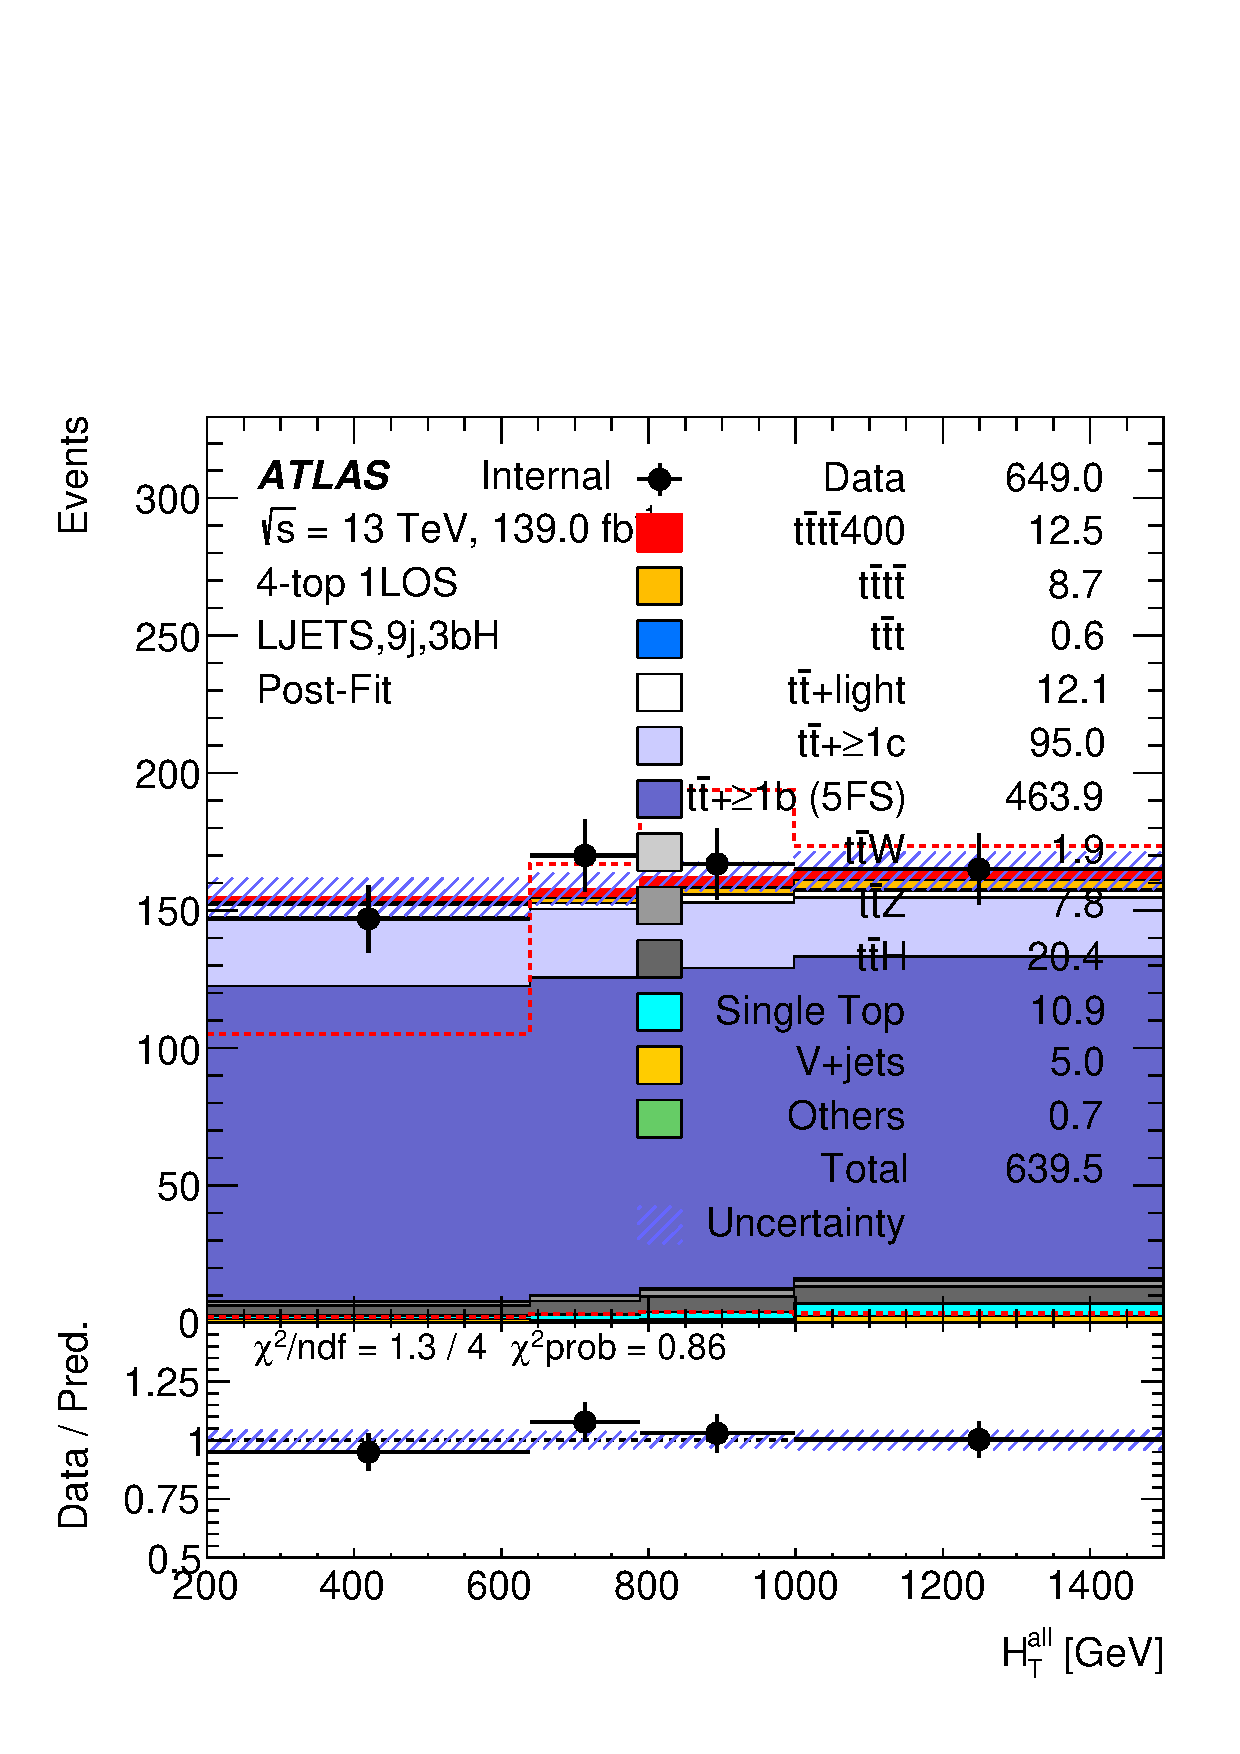
\includegraphics[width=0.23 \textwidth]{figures/fits/GNN/400/all/data_unblindedSplusB/Plots/ljets_9j3bH_postFit.pdf} &
        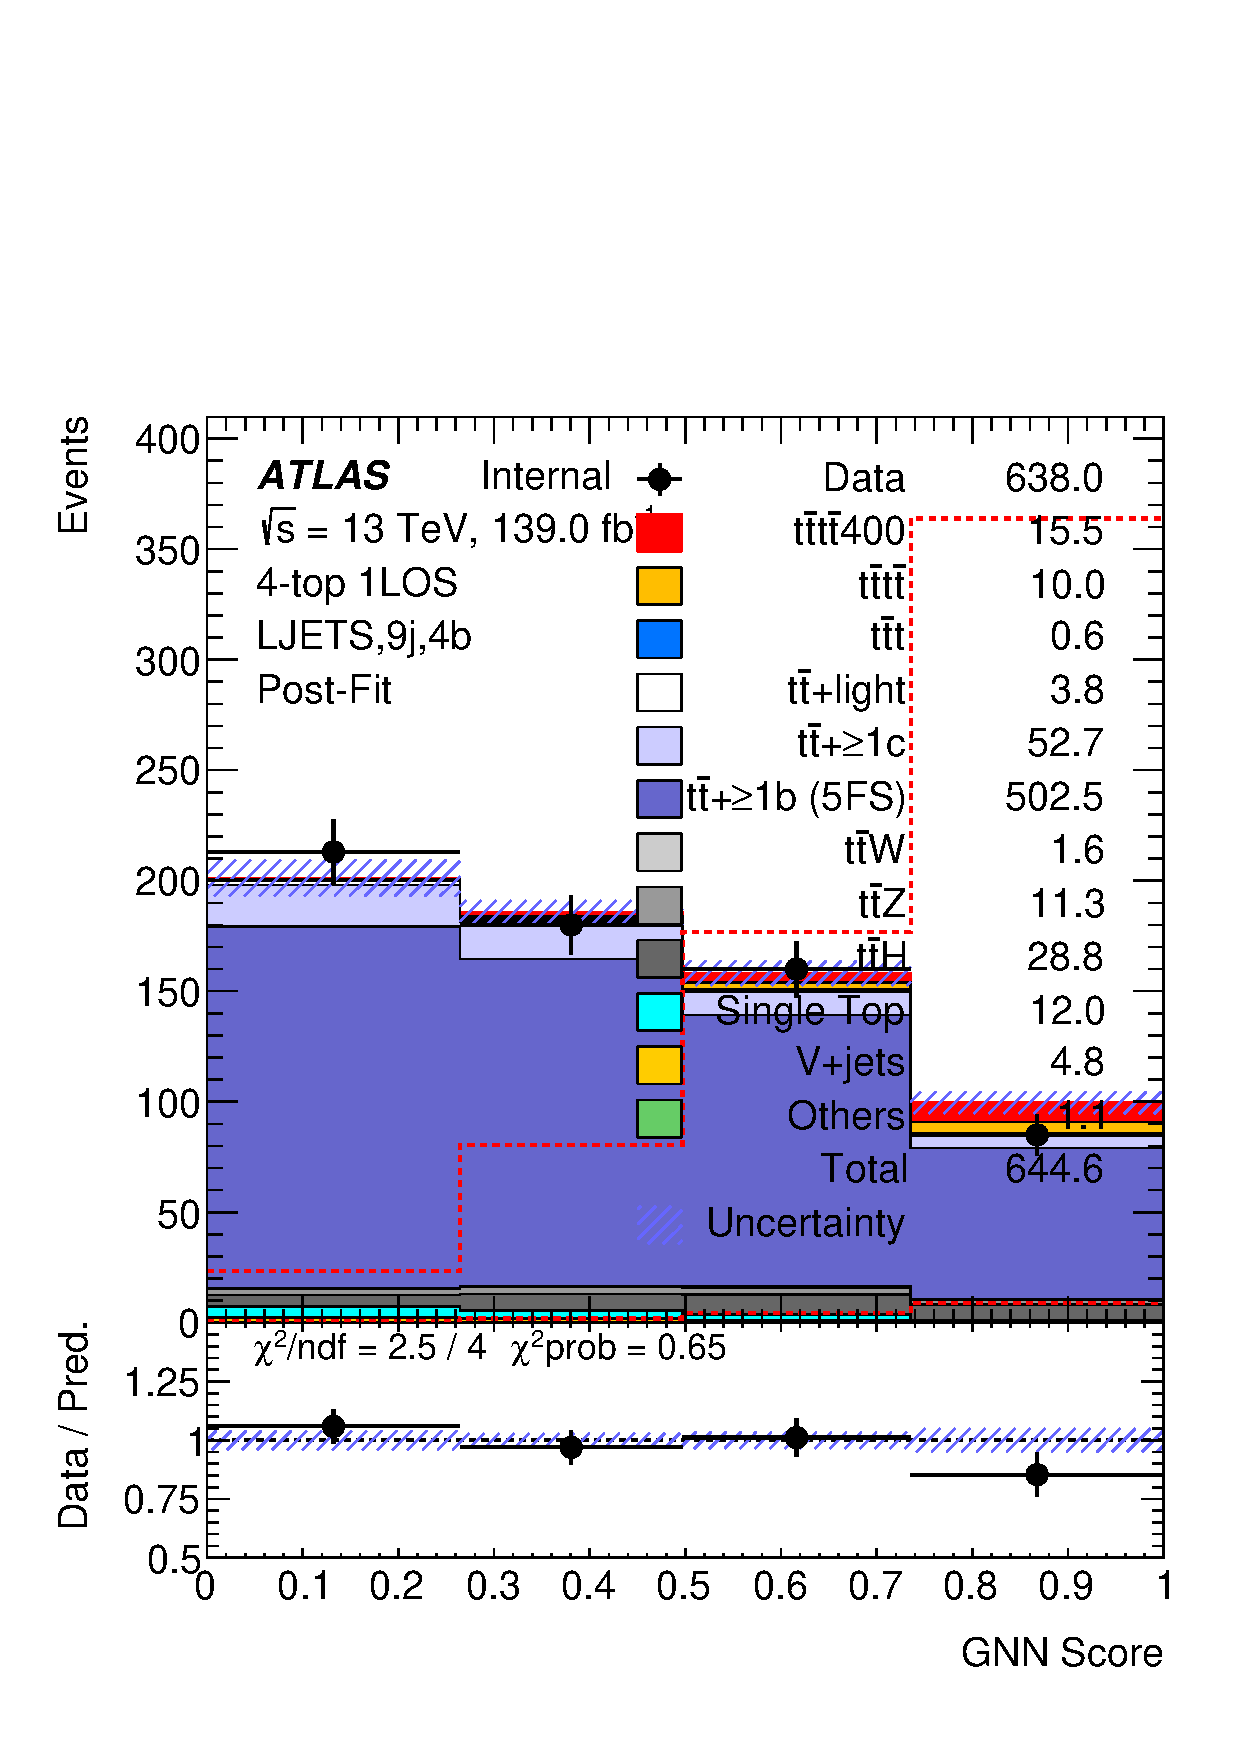
\includegraphics[width=0.23 \textwidth]{figures/fits/GNN/400/all/data_unblindedSplusB/Plots/ljets_9j4b_postFit.pdf} &
        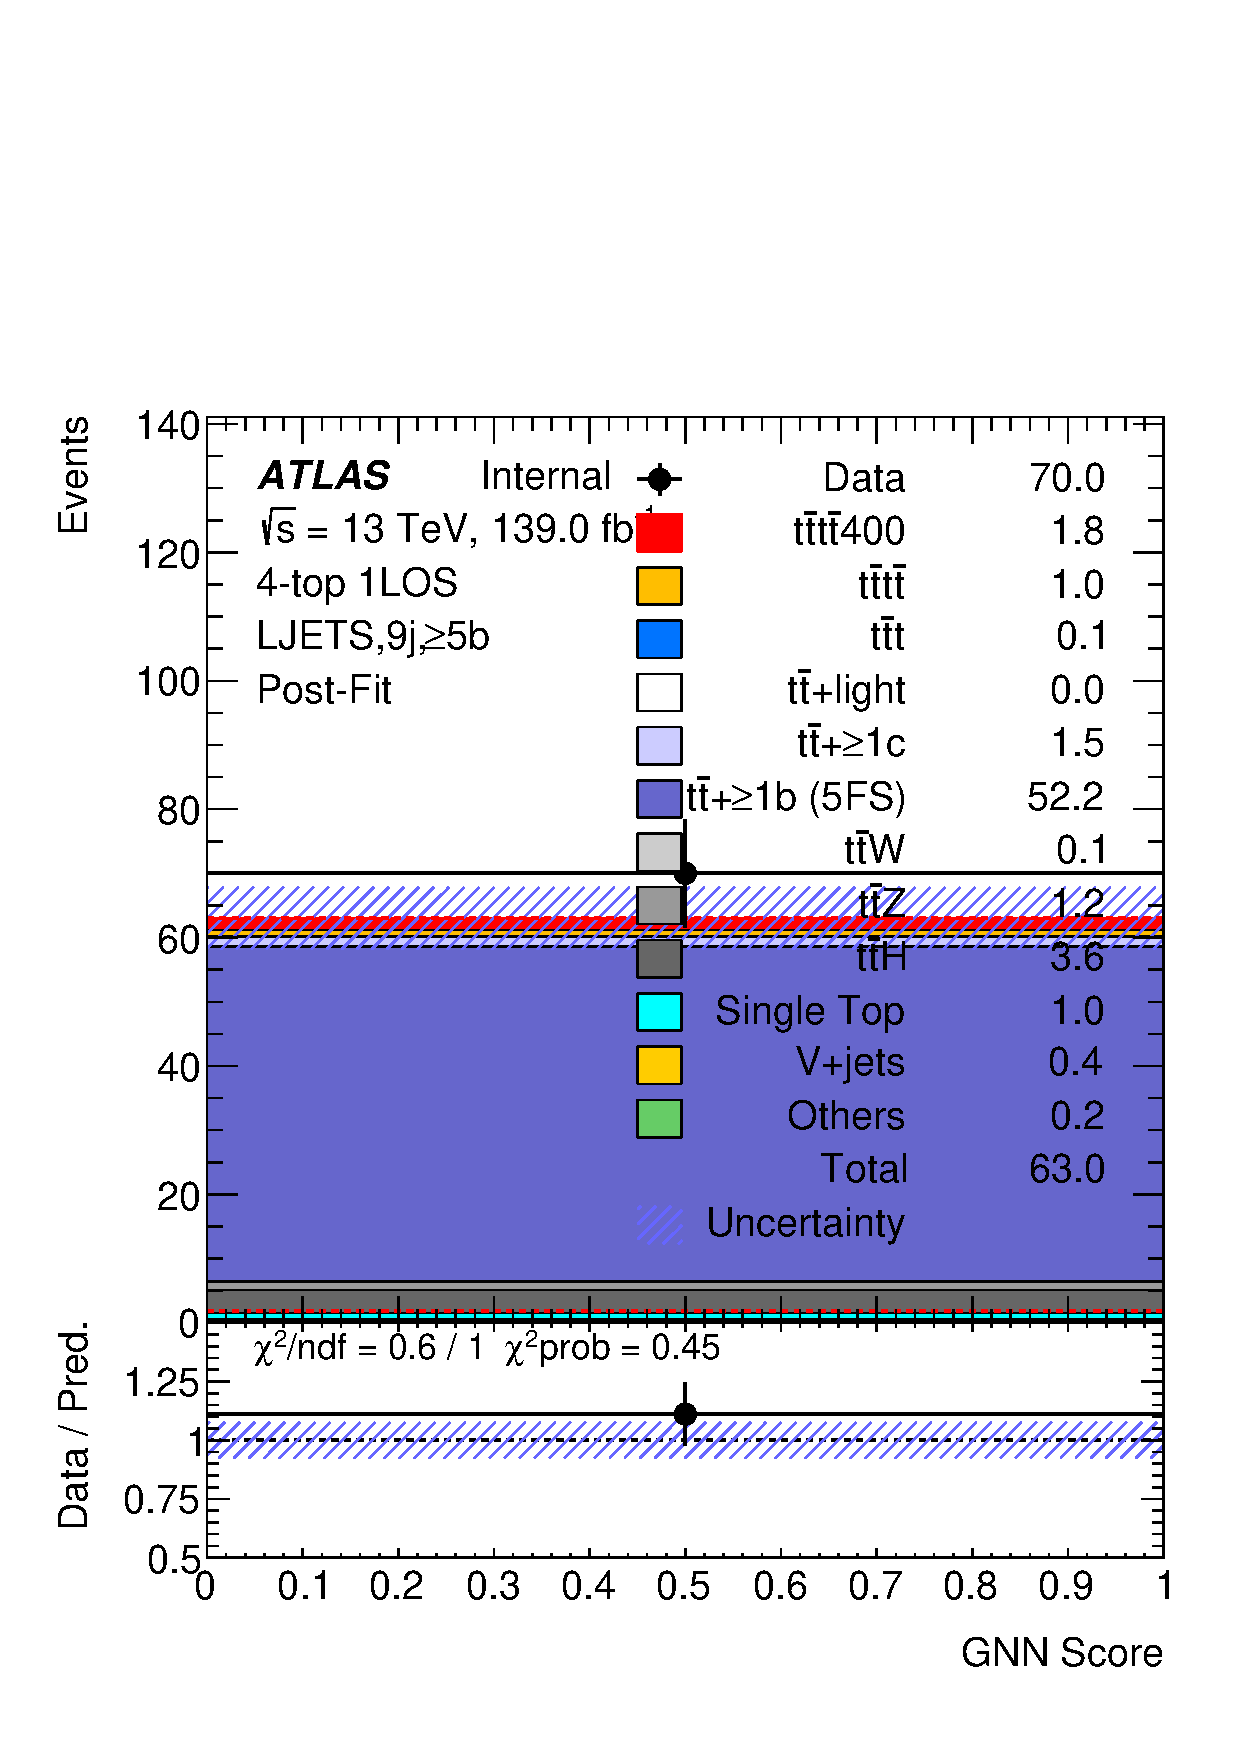
\includegraphics[width=0.23 \textwidth]{figures/fits/GNN/400/all/data_unblindedSplusB/Plots/ljets_9jge5b_postFit.pdf} \\

        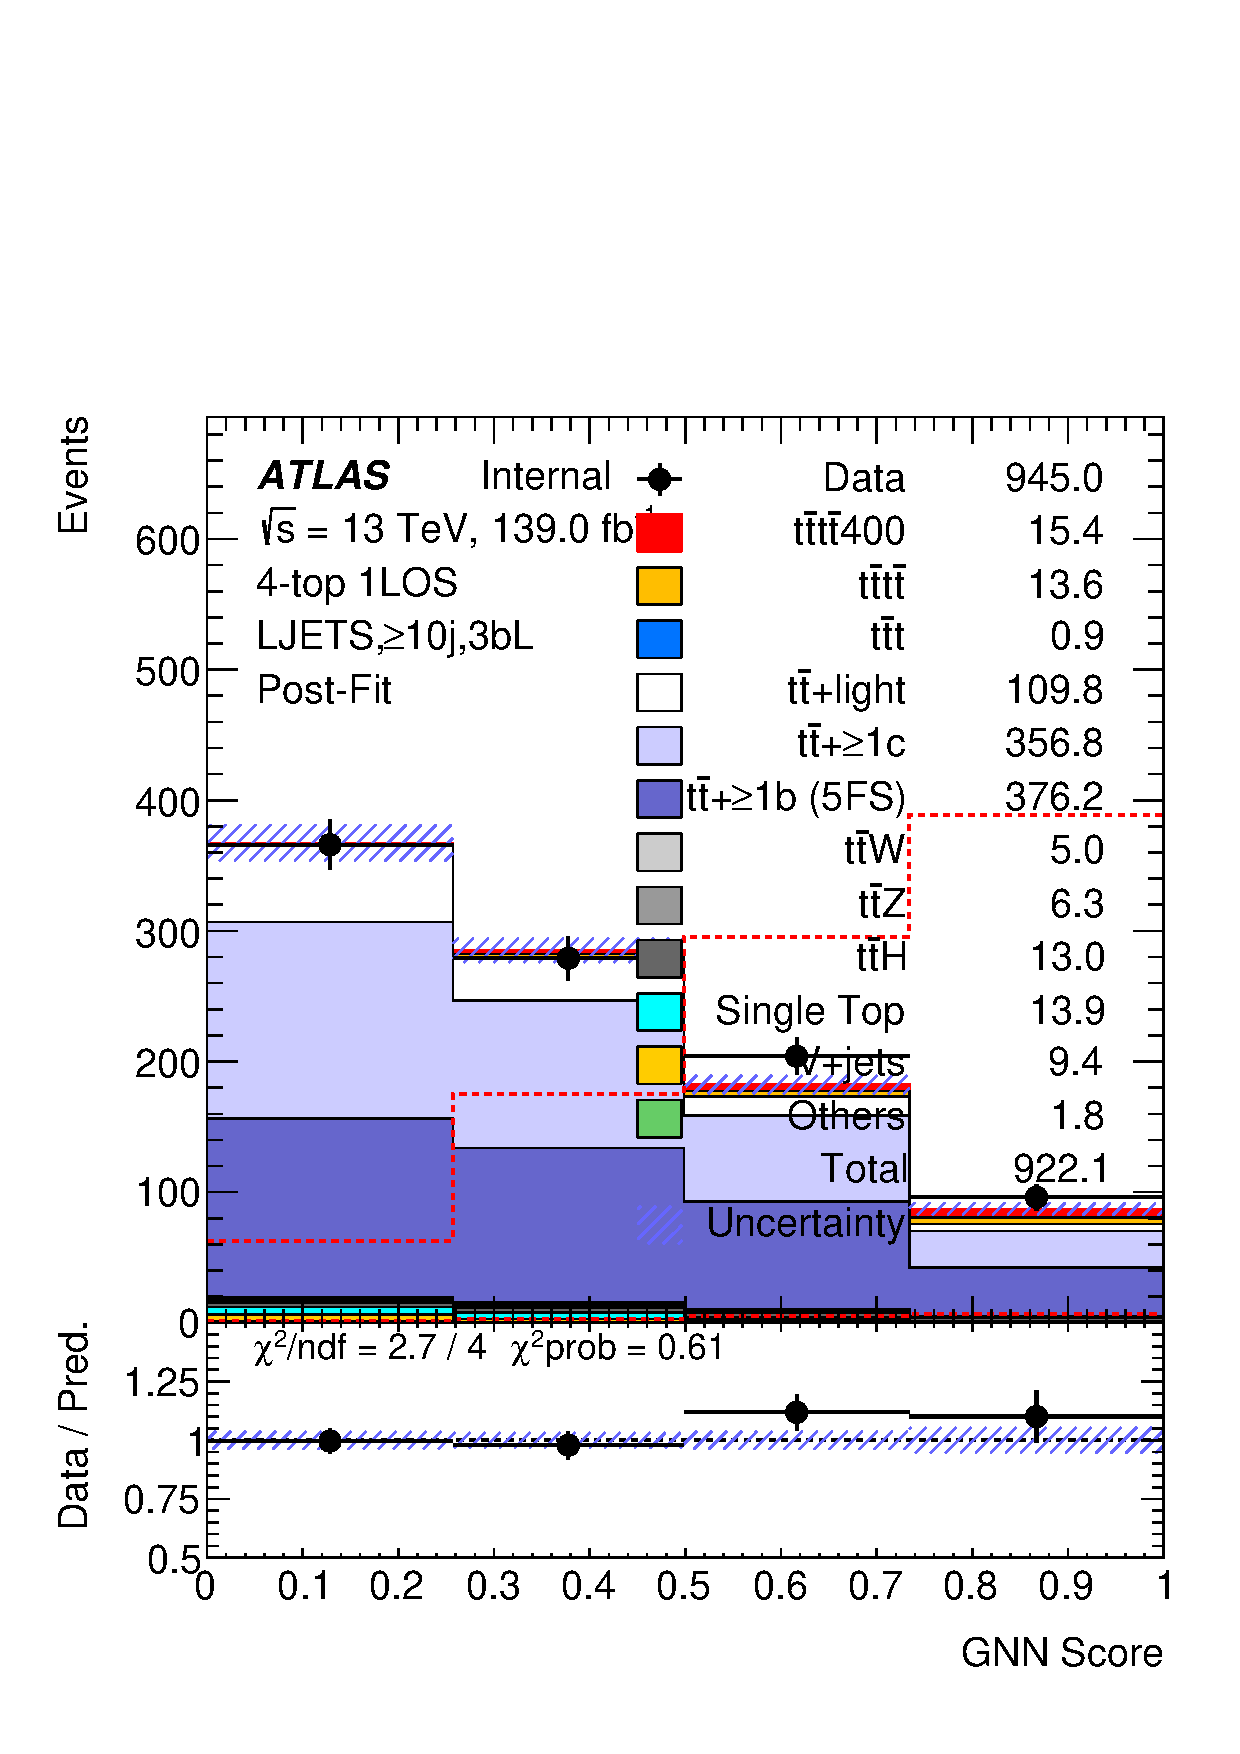
\includegraphics[width=0.23 \textwidth]{figures/fits/GNN/400/all/data_unblindedSplusB/Plots/ljets_ge10j3bL_postFit.pdf} &
        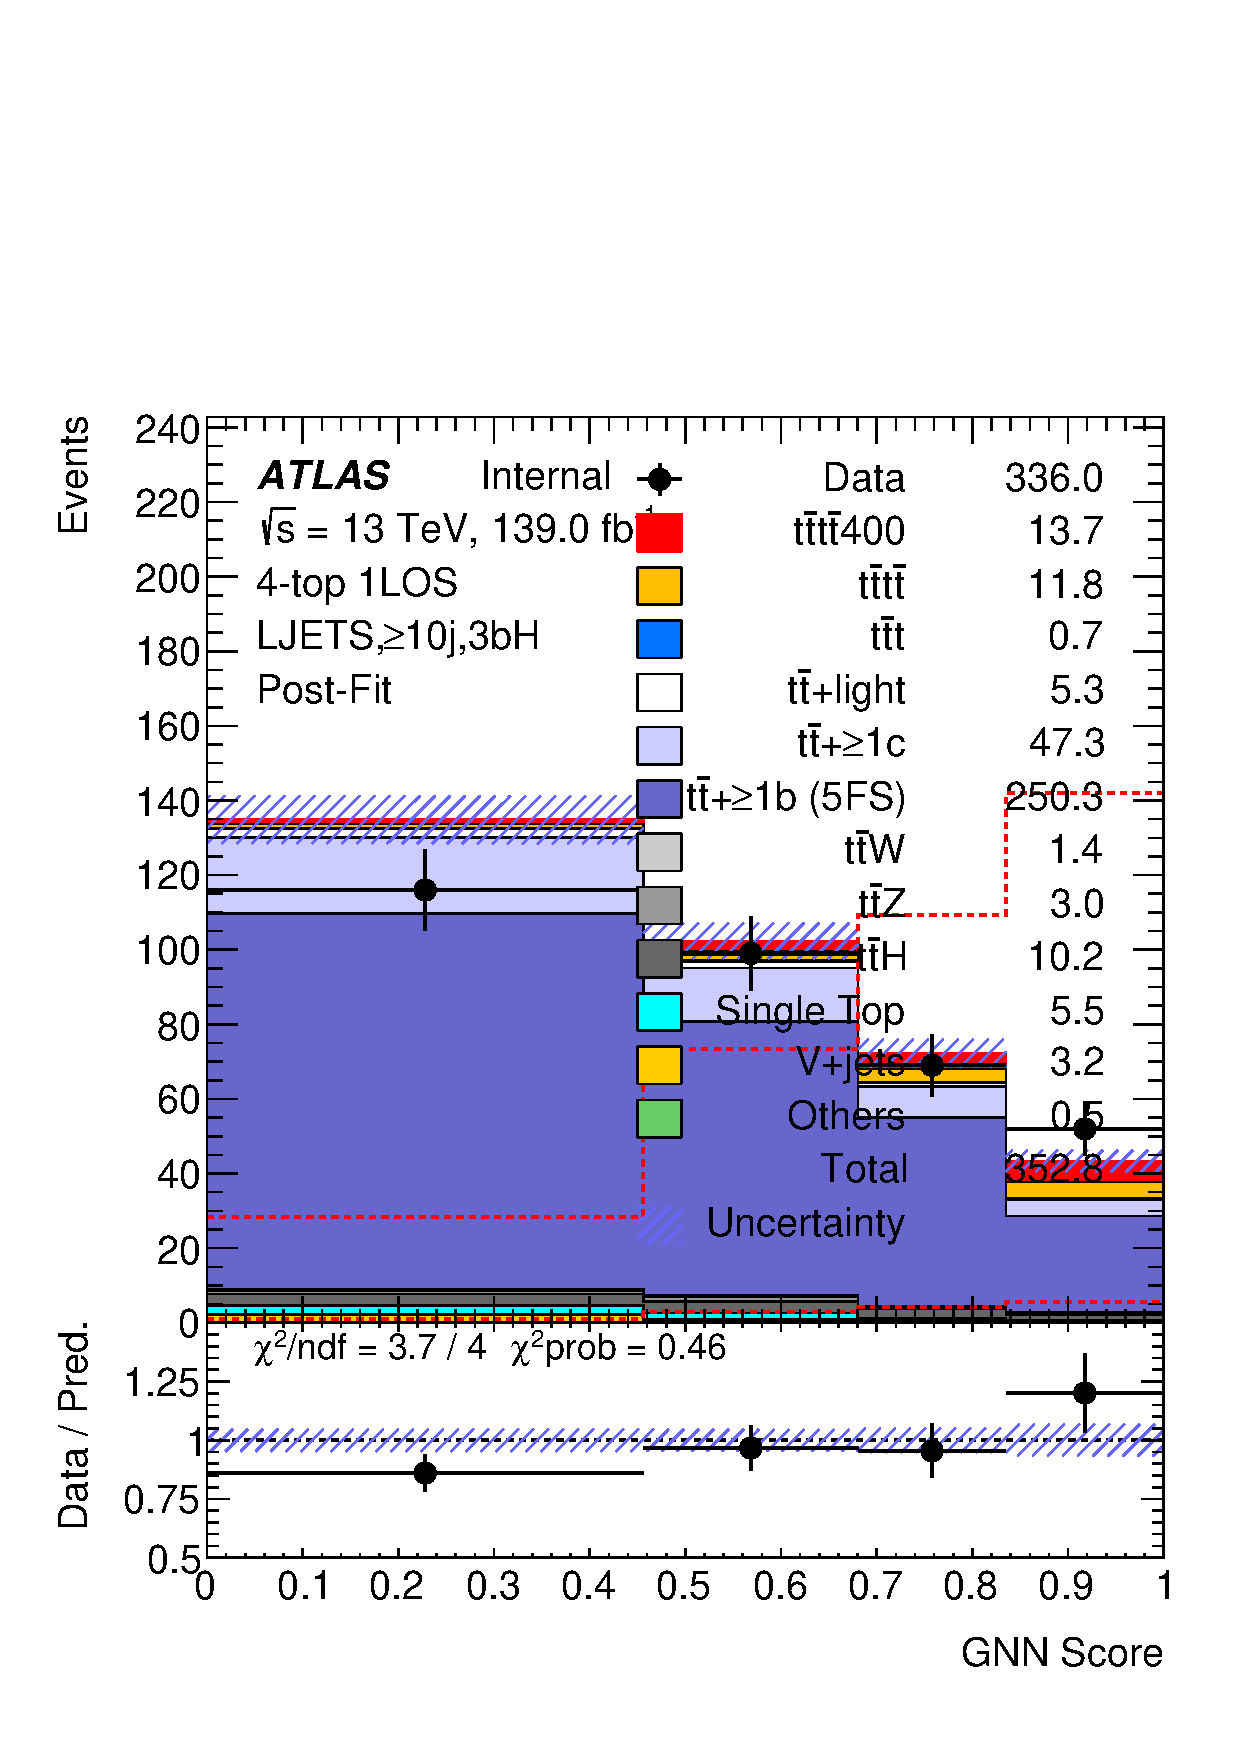
\includegraphics[width=0.23 \textwidth]{figures/fits/GNN/400/all/data_unblindedSplusB/Plots/ljets_ge10j3bH_postFit.pdf} &
        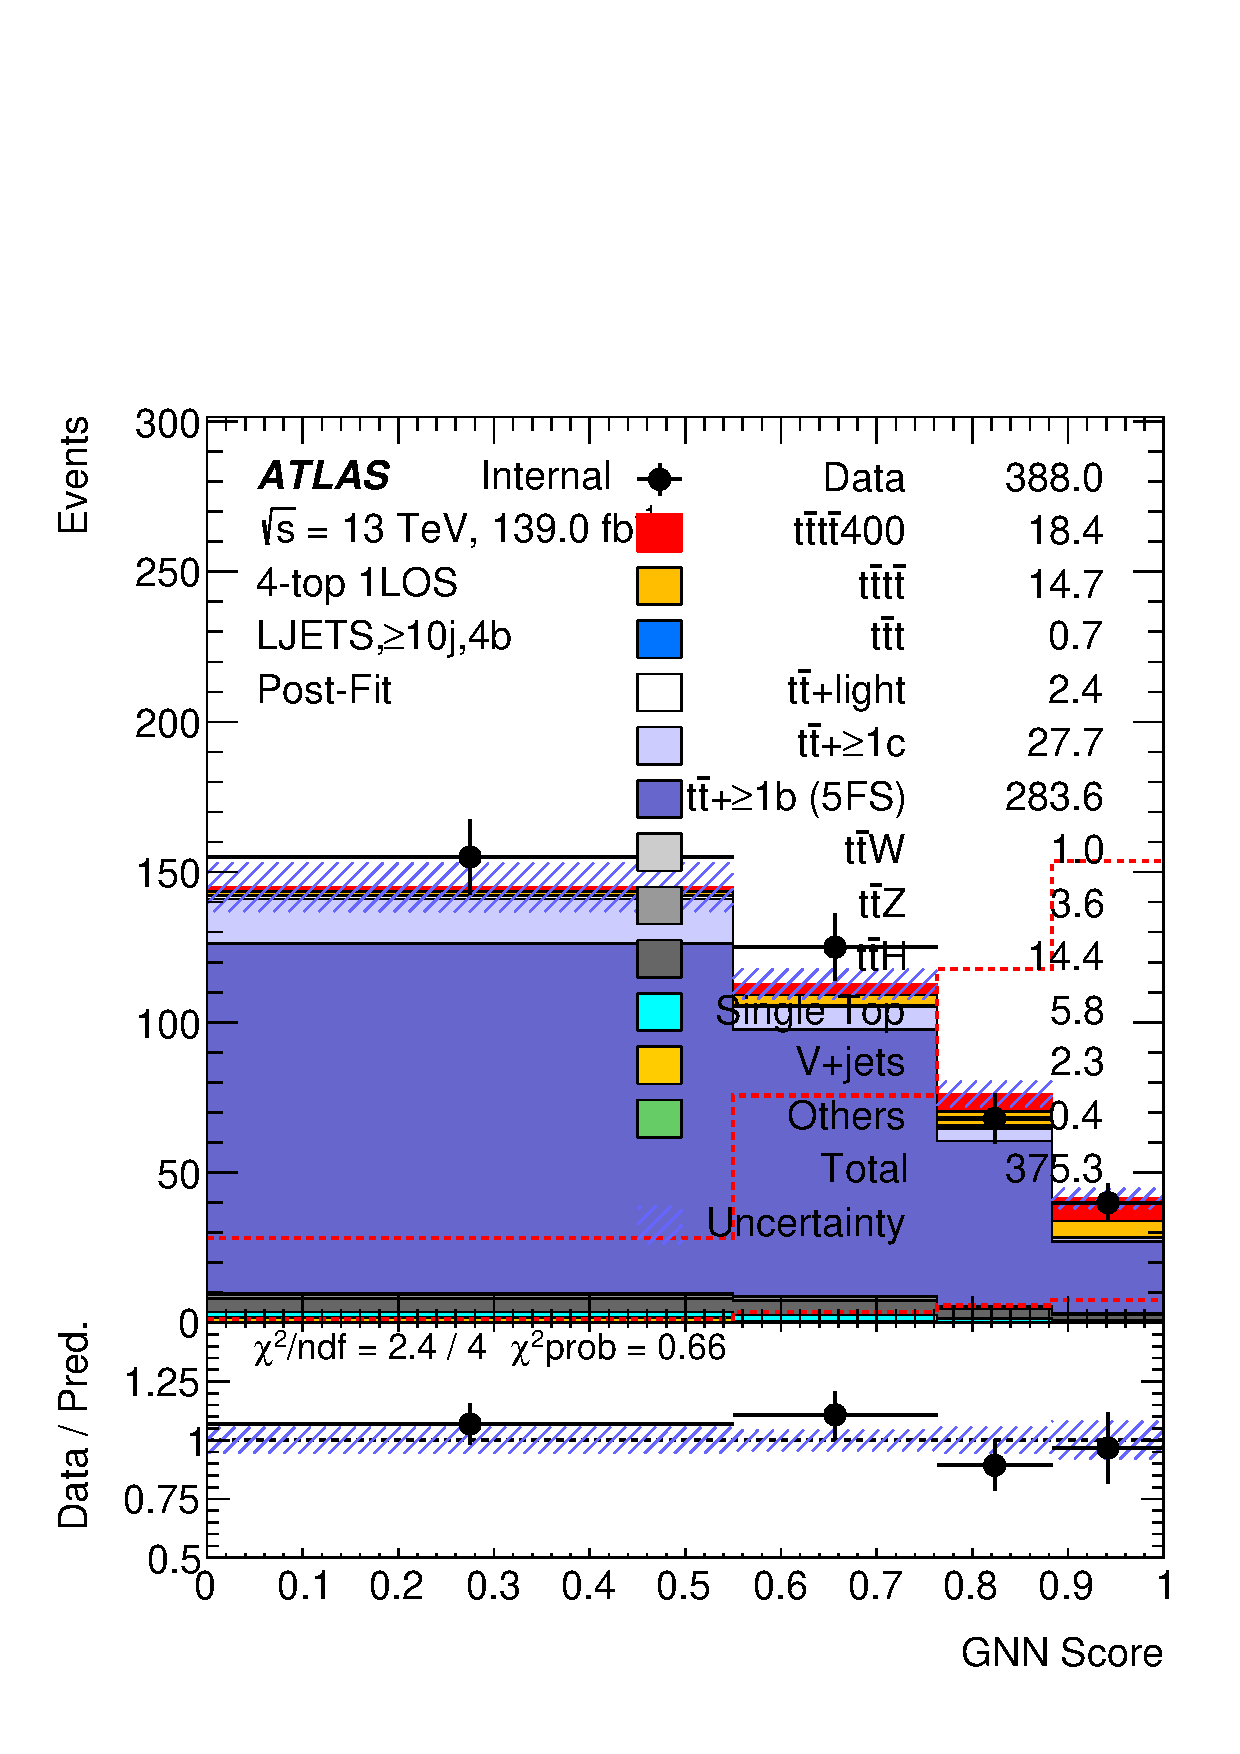
\includegraphics[width=0.23 \textwidth]{figures/fits/GNN/400/all/data_unblindedSplusB/Plots/ljets_ge10j4b_postFit.pdf} &
        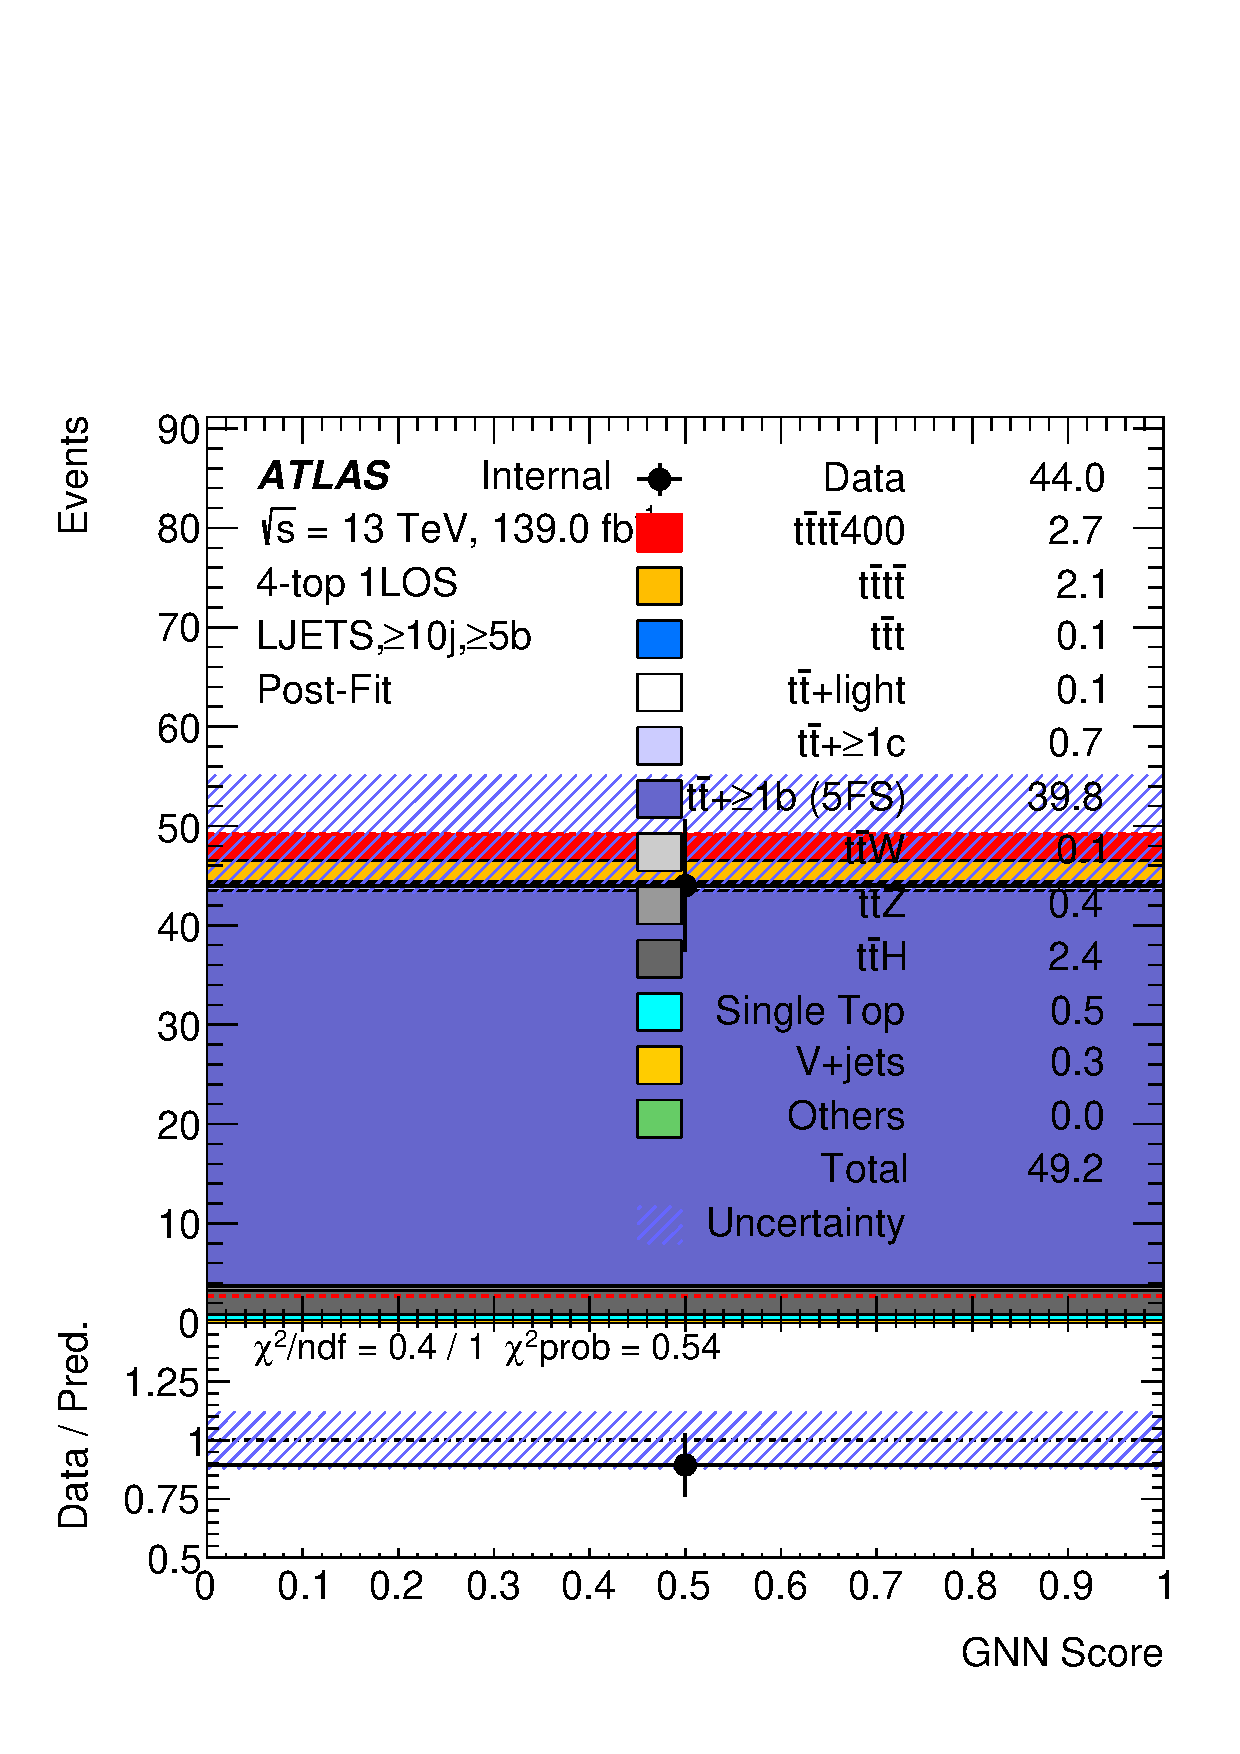
\includegraphics[width=0.23 \textwidth]{figures/fits/GNN/400/all/data_unblindedSplusB/Plots/ljets_ge10jge5b_postFit.pdf} \\
        \end{tabular}
        \caption{\label{fig:unblinded_data_SplusB_postfit_1L}
        Post-fit distributions for the 1L regions obtained from the unblinded signal-plus-background data fit at $\boldsymbol{m_H=400}$~GeV. 
        The fit is performed using all regions (1L+2LOS).}
\end{center}
\end{figure}

\begin{figure}[htbp!]
        \begin{center} \setlength{\tabcolsep}{2.5pt}\footnotesize
        \begin{tabular}{ccc}
        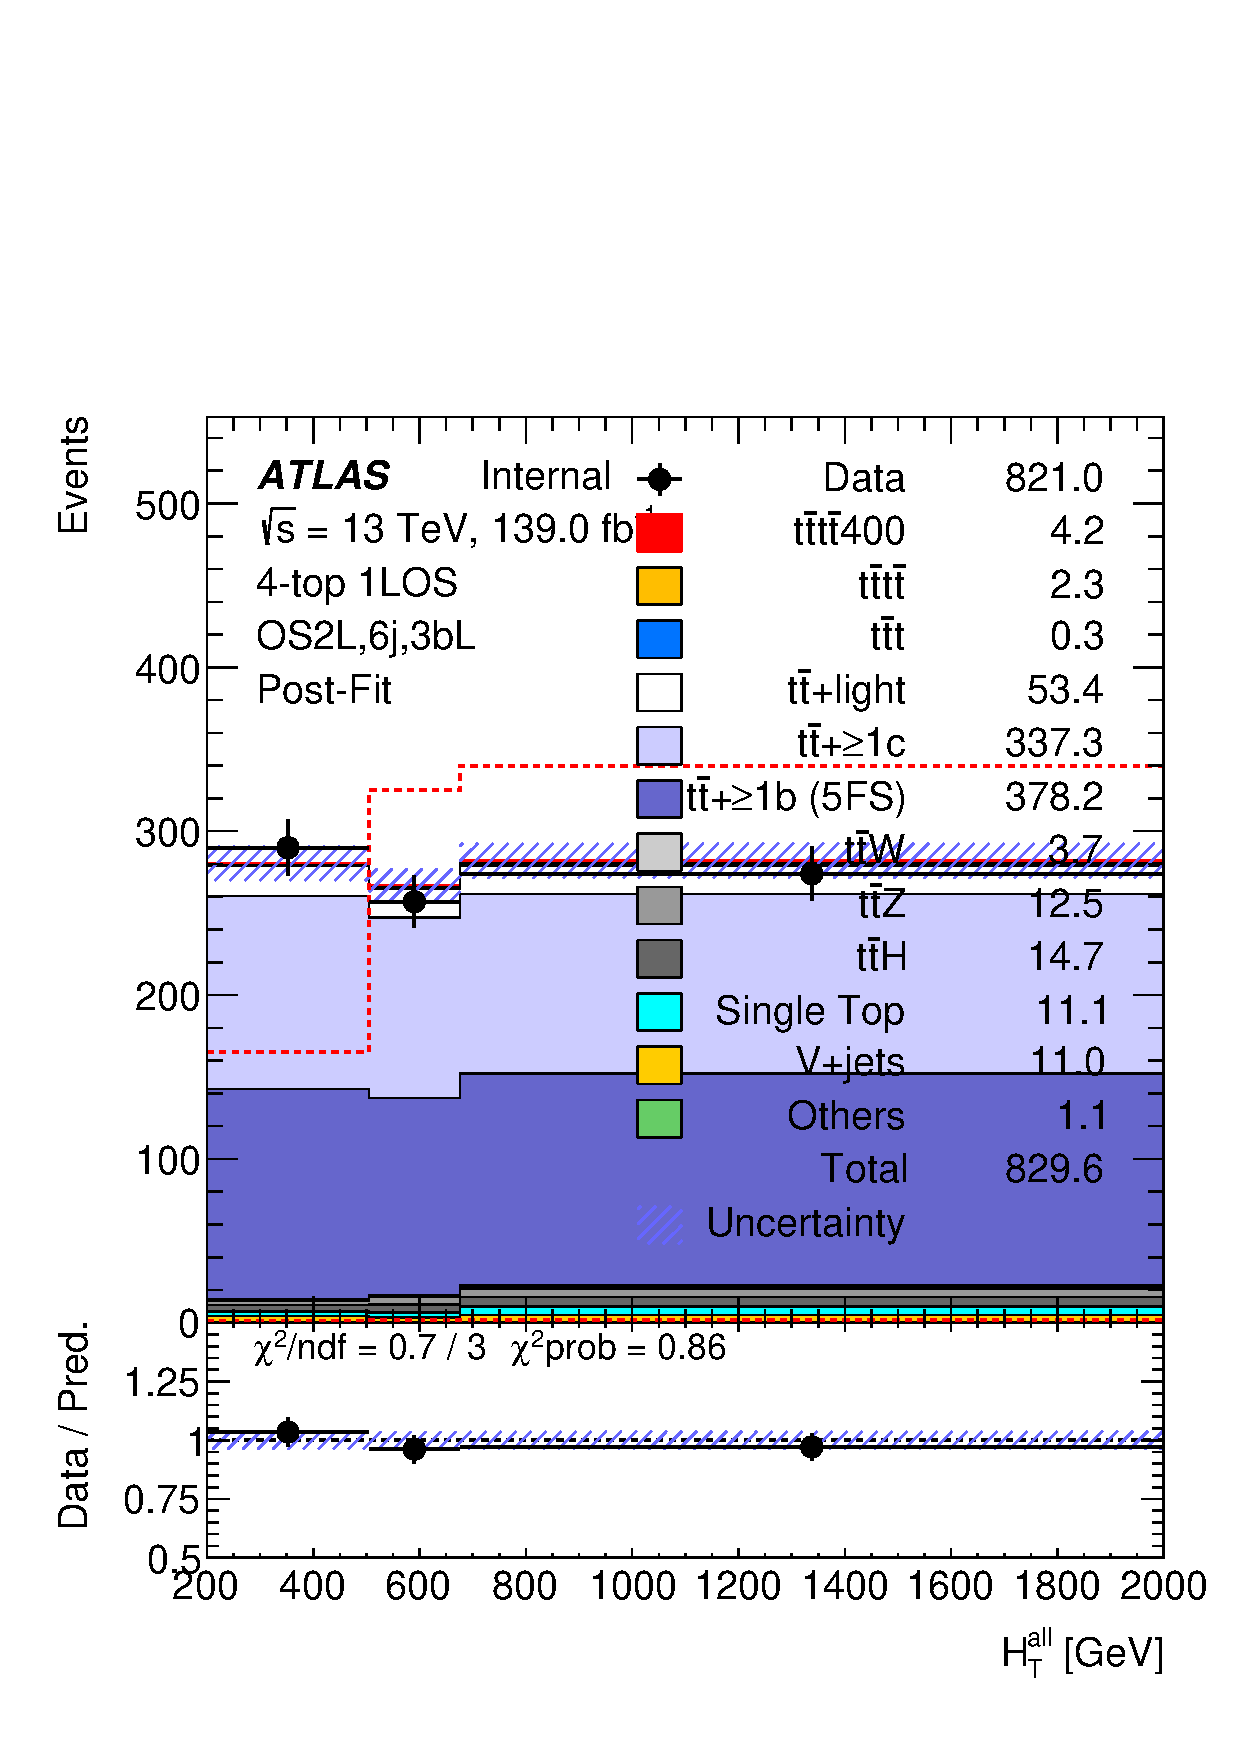
\includegraphics[width=0.31 \textwidth]{figures/fits/GNN/400/all/data_unblindedSplusB/Plots/os2l_6j3bL_postFit.pdf} &
        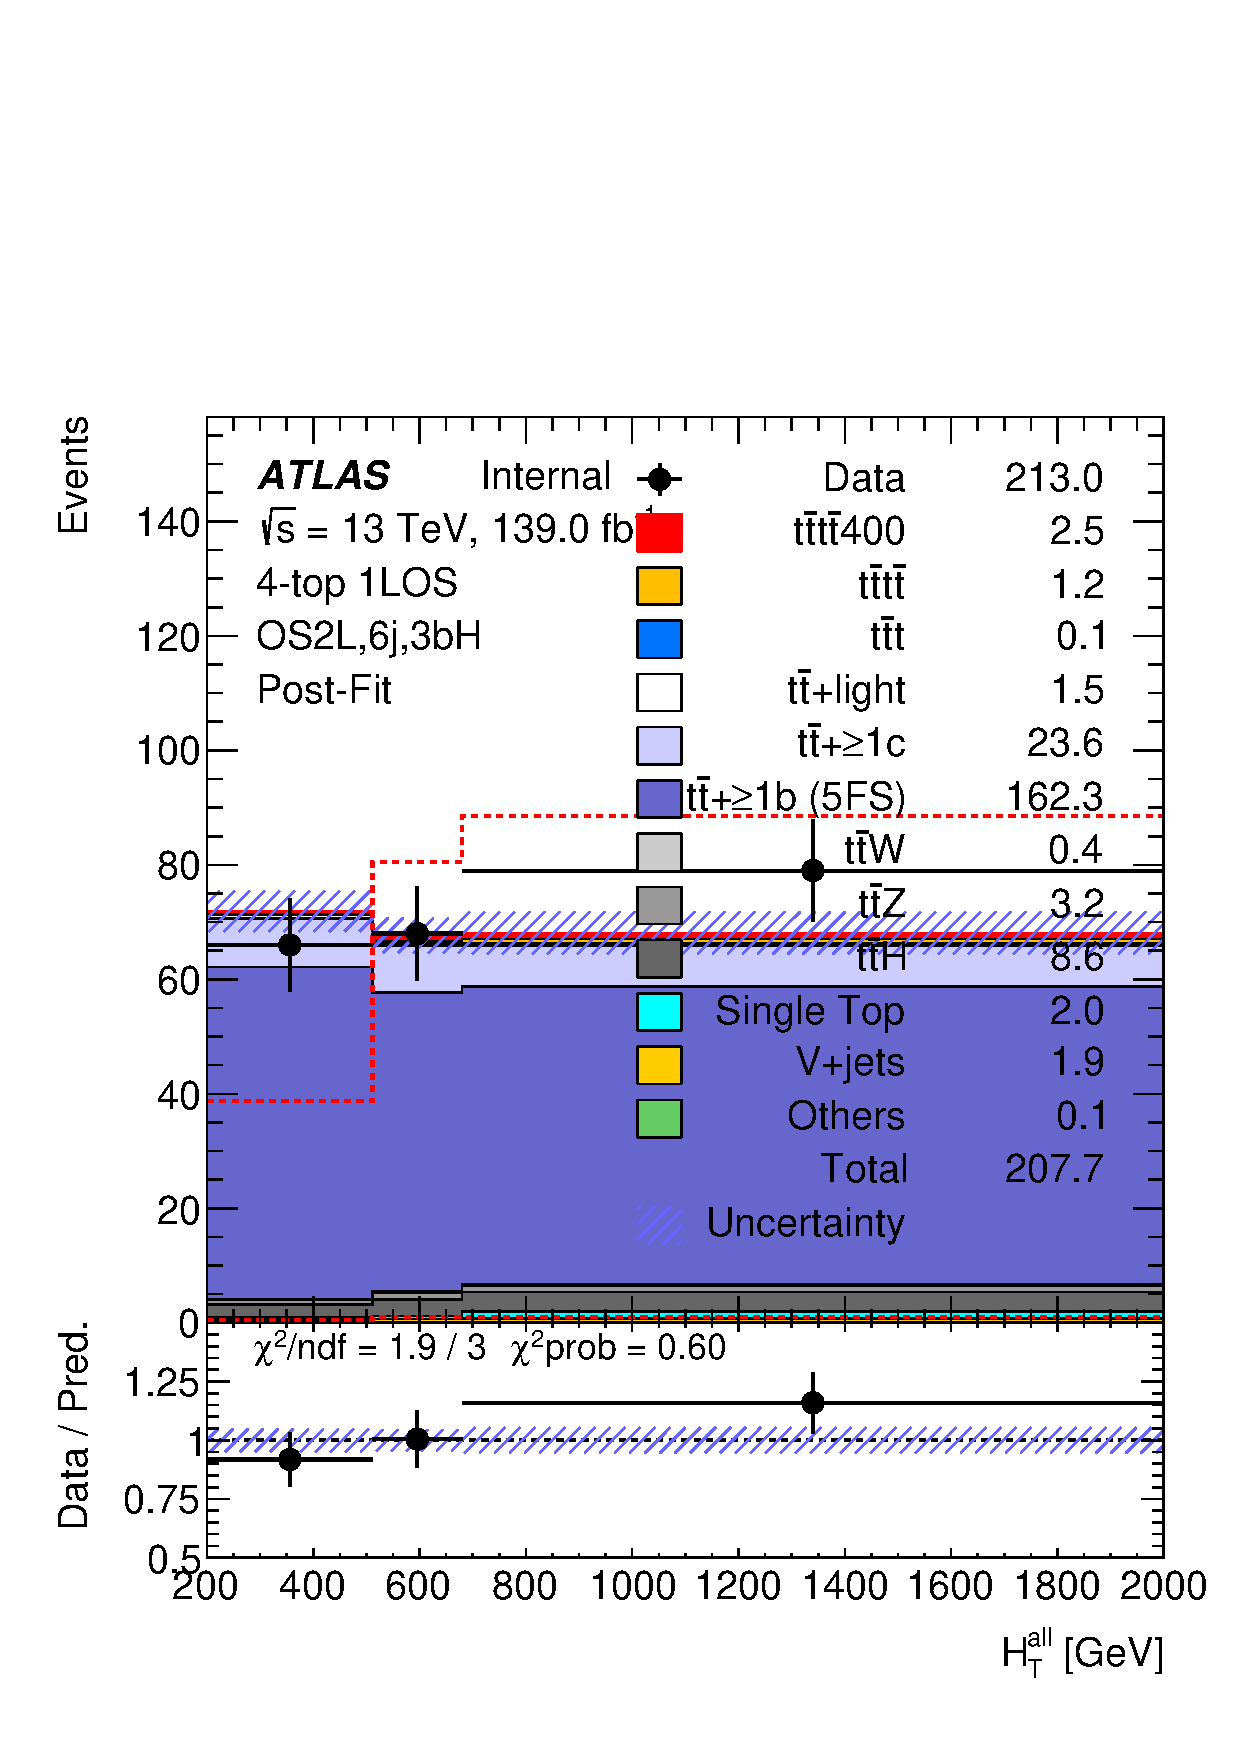
\includegraphics[width=0.31 \textwidth]{figures/fits/GNN/400/all/data_unblindedSplusB/Plots/os2l_6j3bH_postFit.pdf} &
        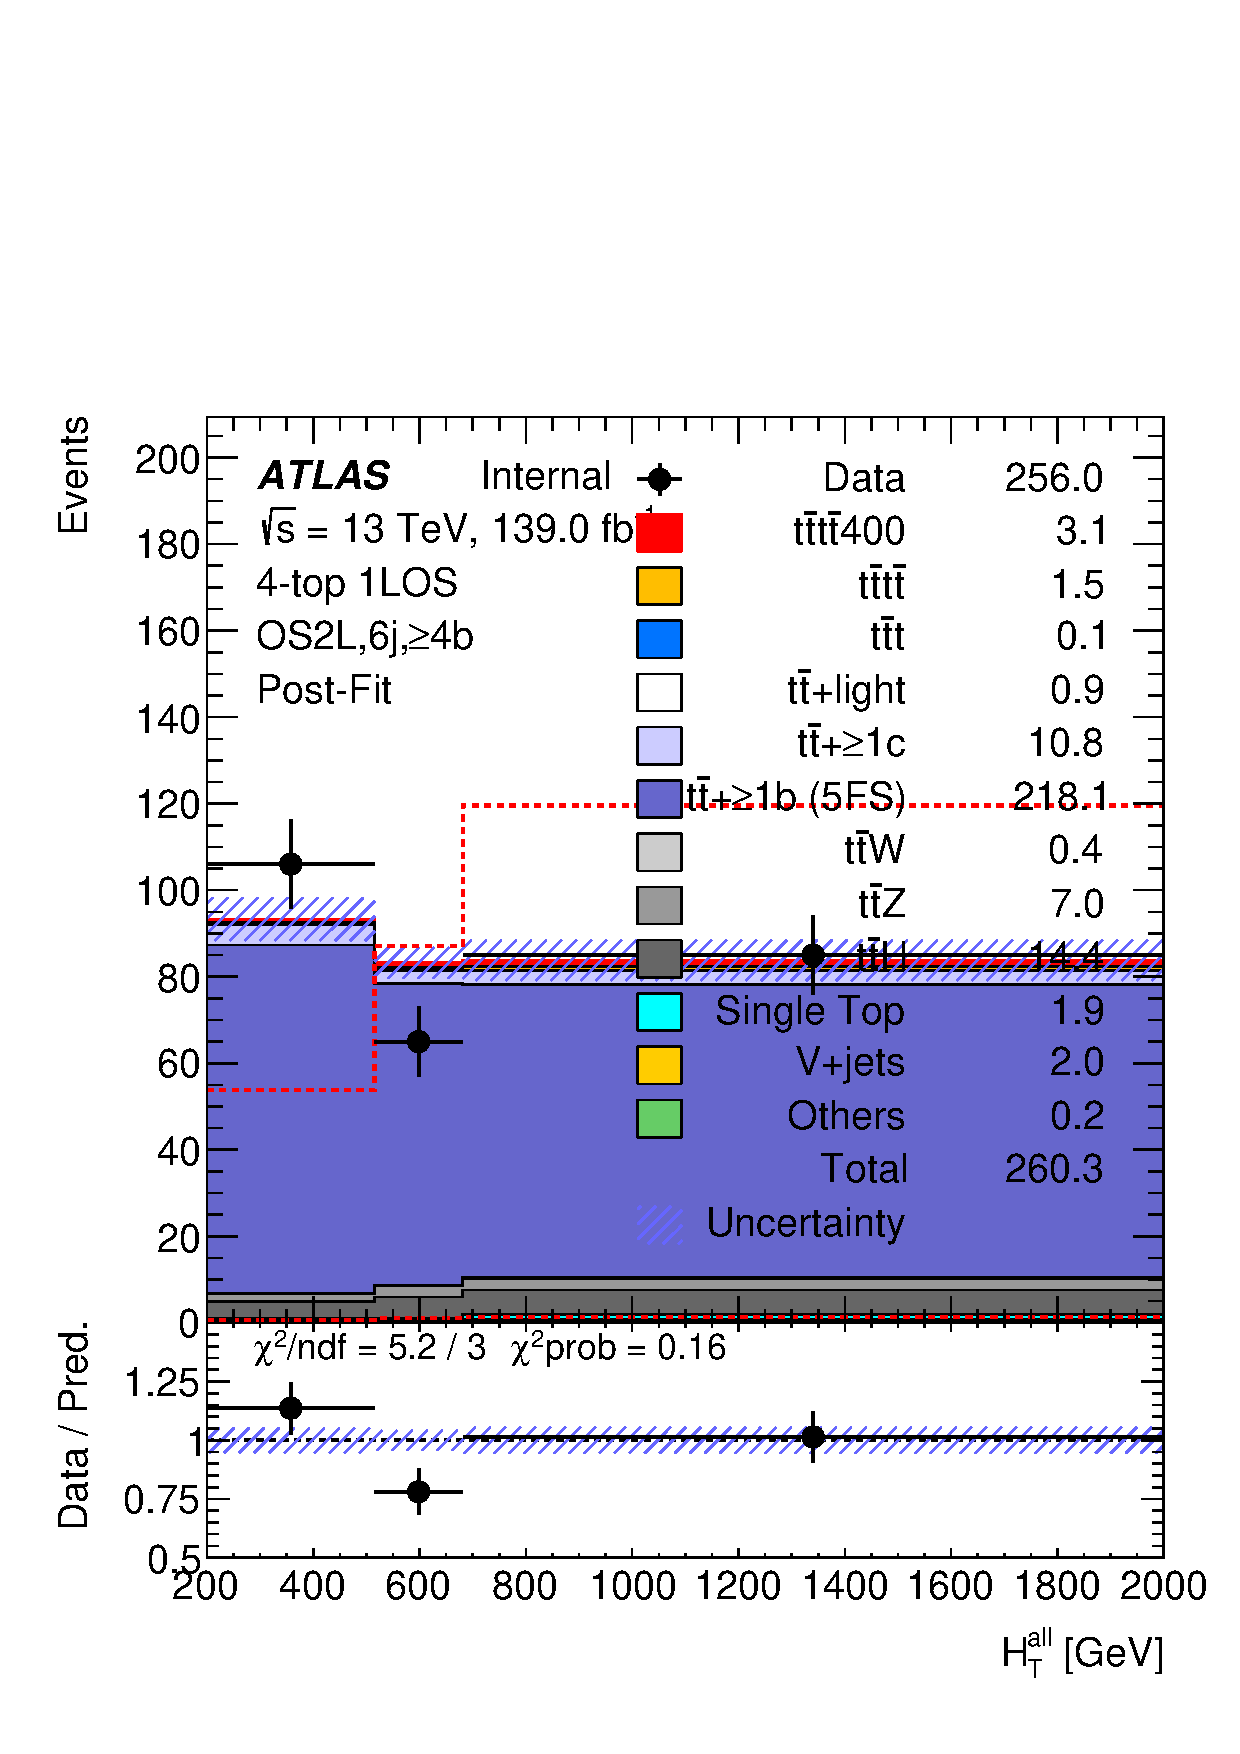
\includegraphics[width=0.31 \textwidth]{figures/fits/GNN/400/all/data_unblindedSplusB/Plots/os2l_6jge4b_postFit.pdf} \\

        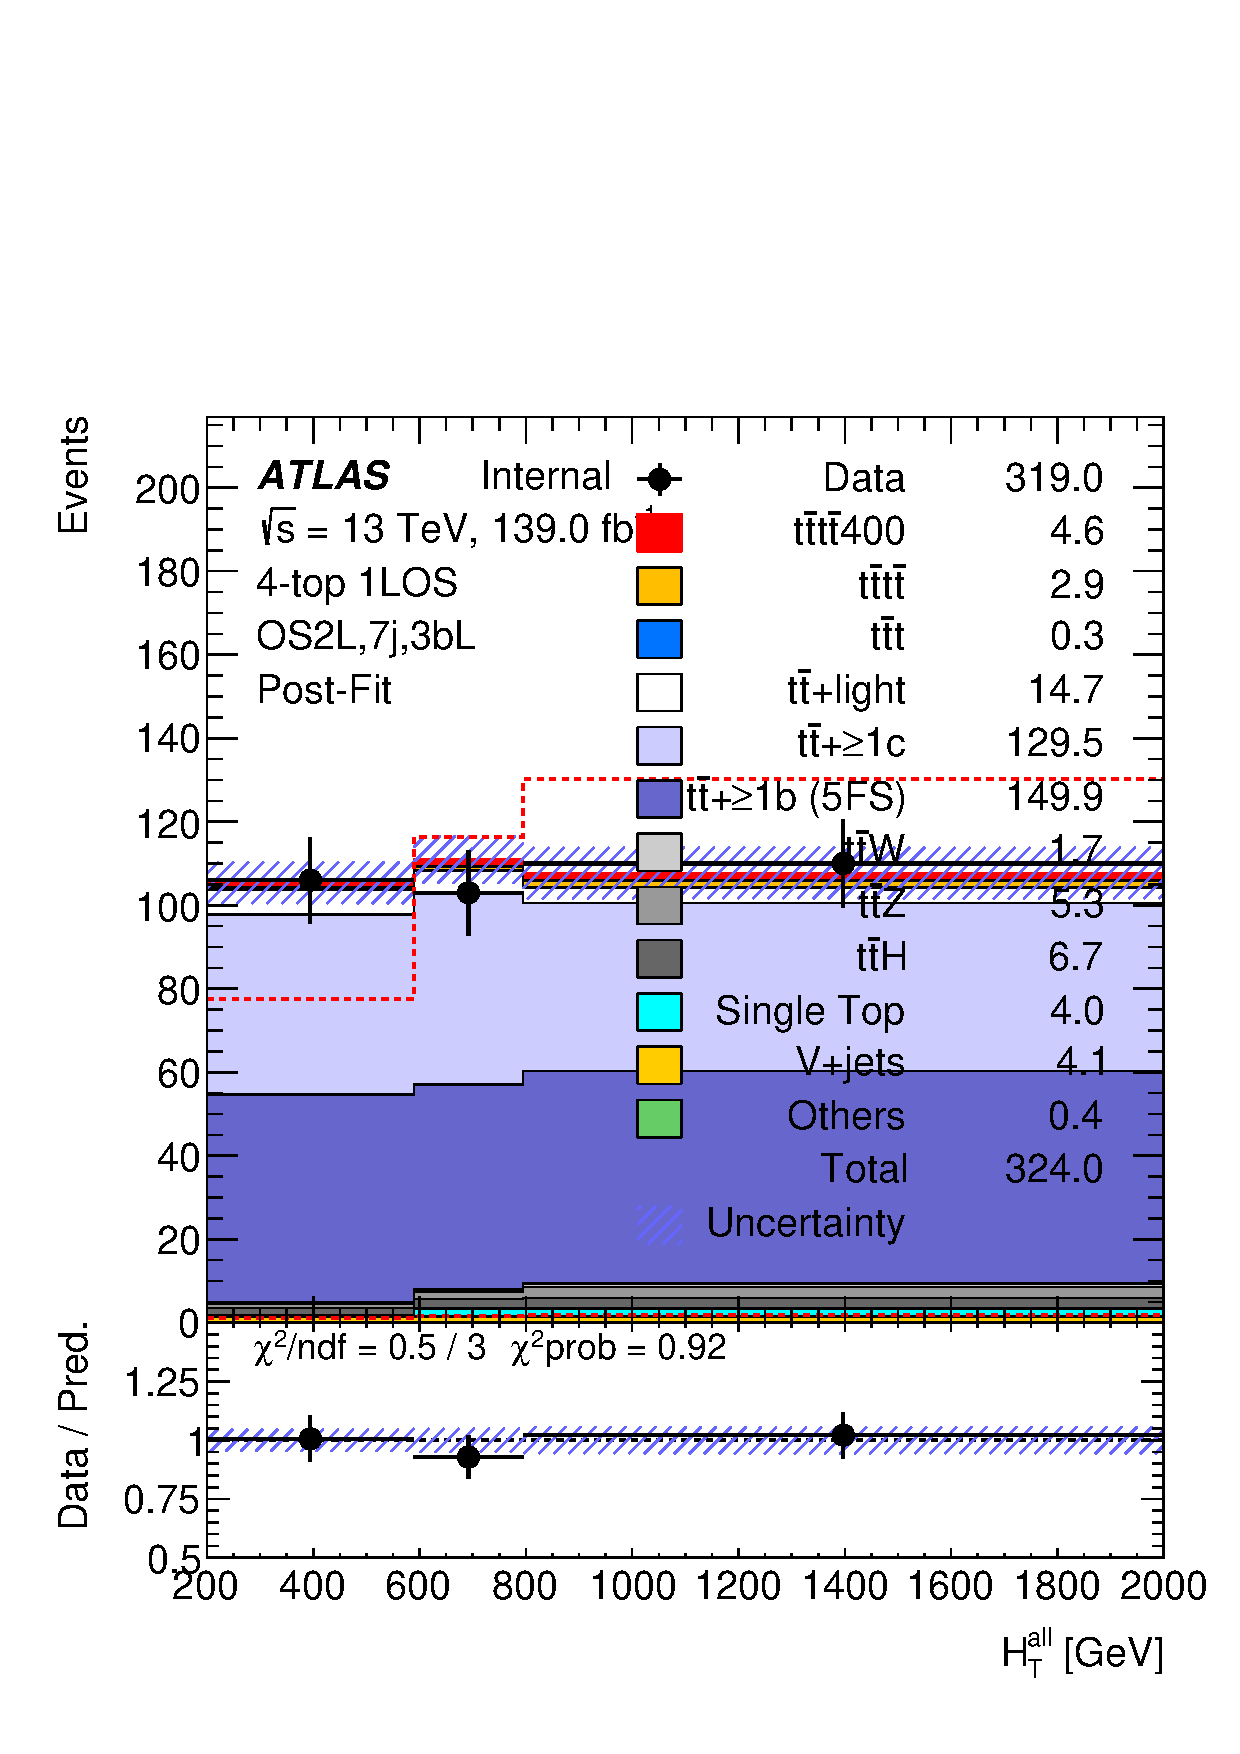
\includegraphics[width=0.31 \textwidth]{figures/fits/GNN/400/all/data_unblindedSplusB/Plots/os2l_7j3bL_postFit.pdf} &
        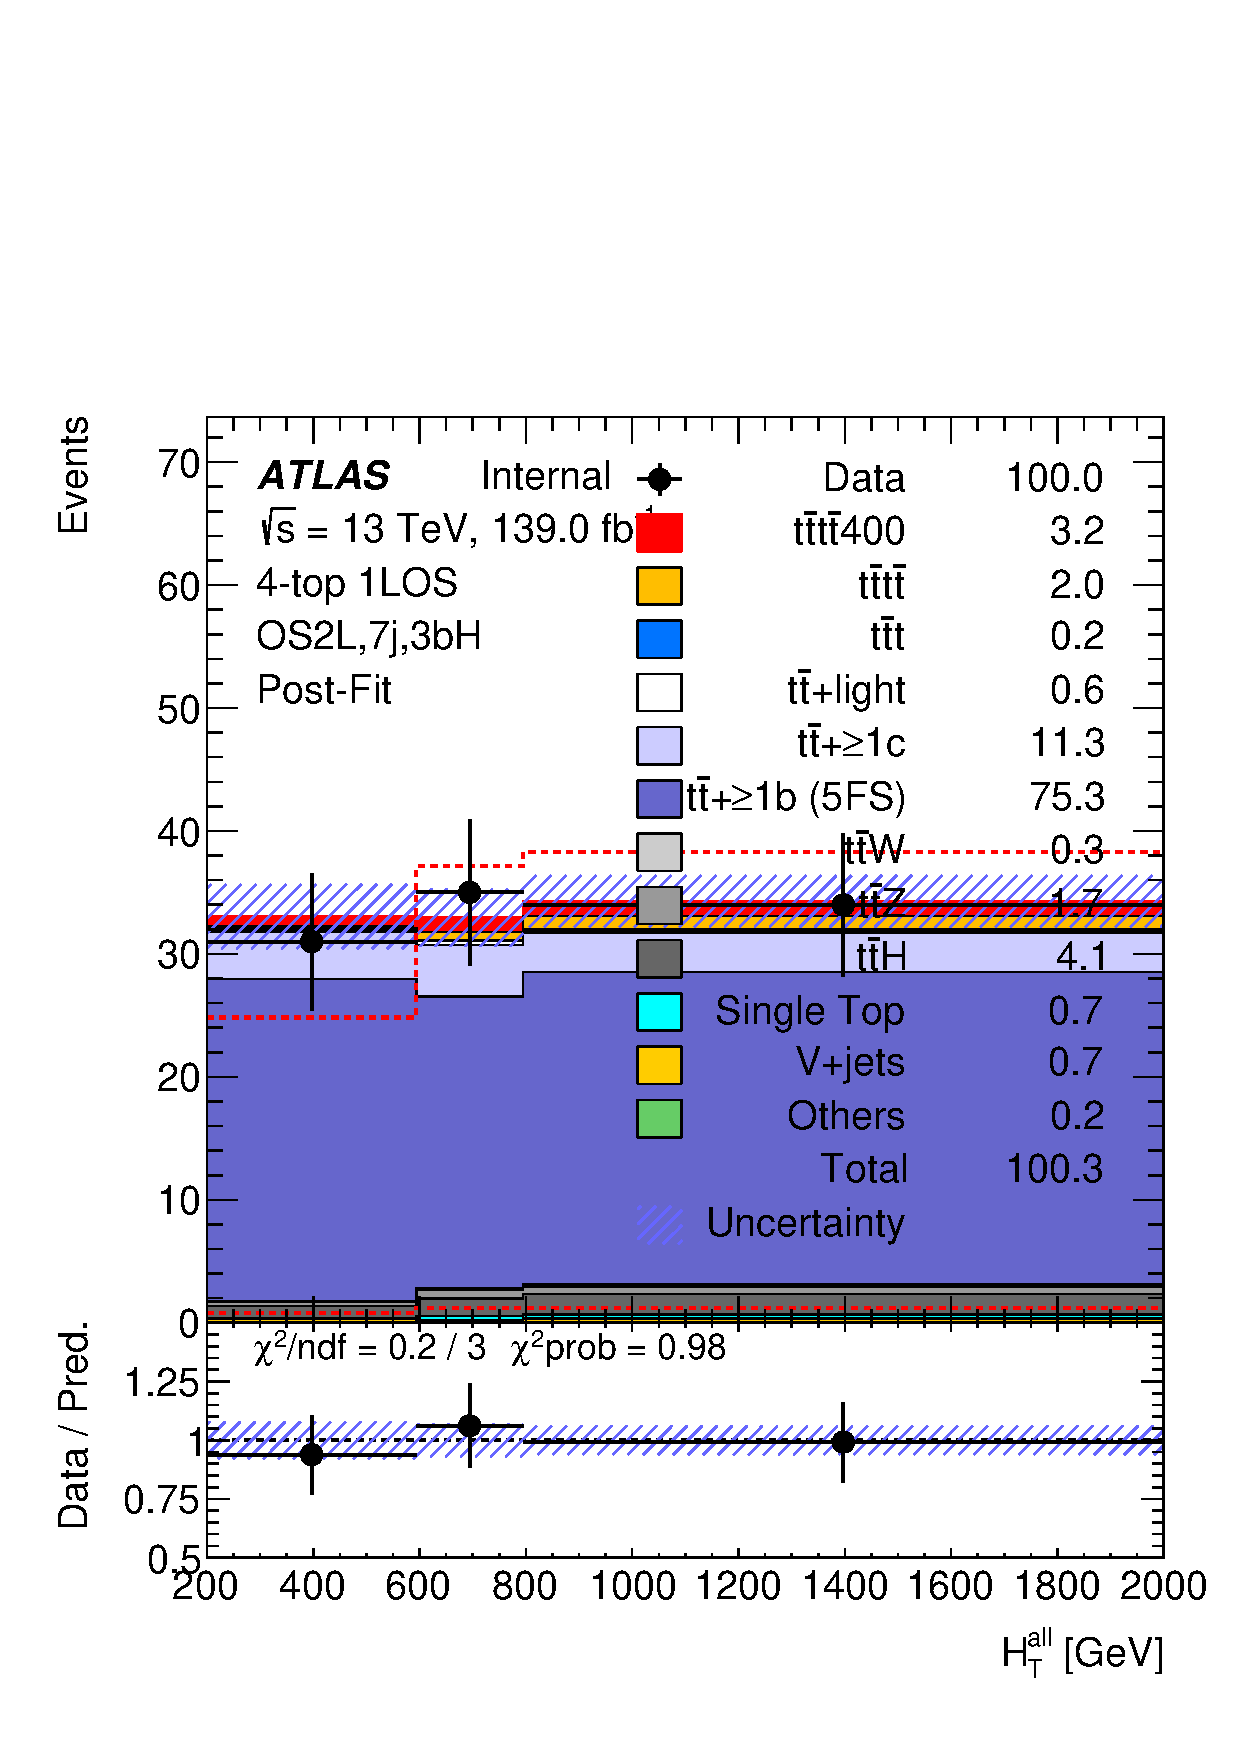
\includegraphics[width=0.31 \textwidth]{figures/fits/GNN/400/all/data_unblindedSplusB/Plots/os2l_7j3bH_postFit.pdf} &
        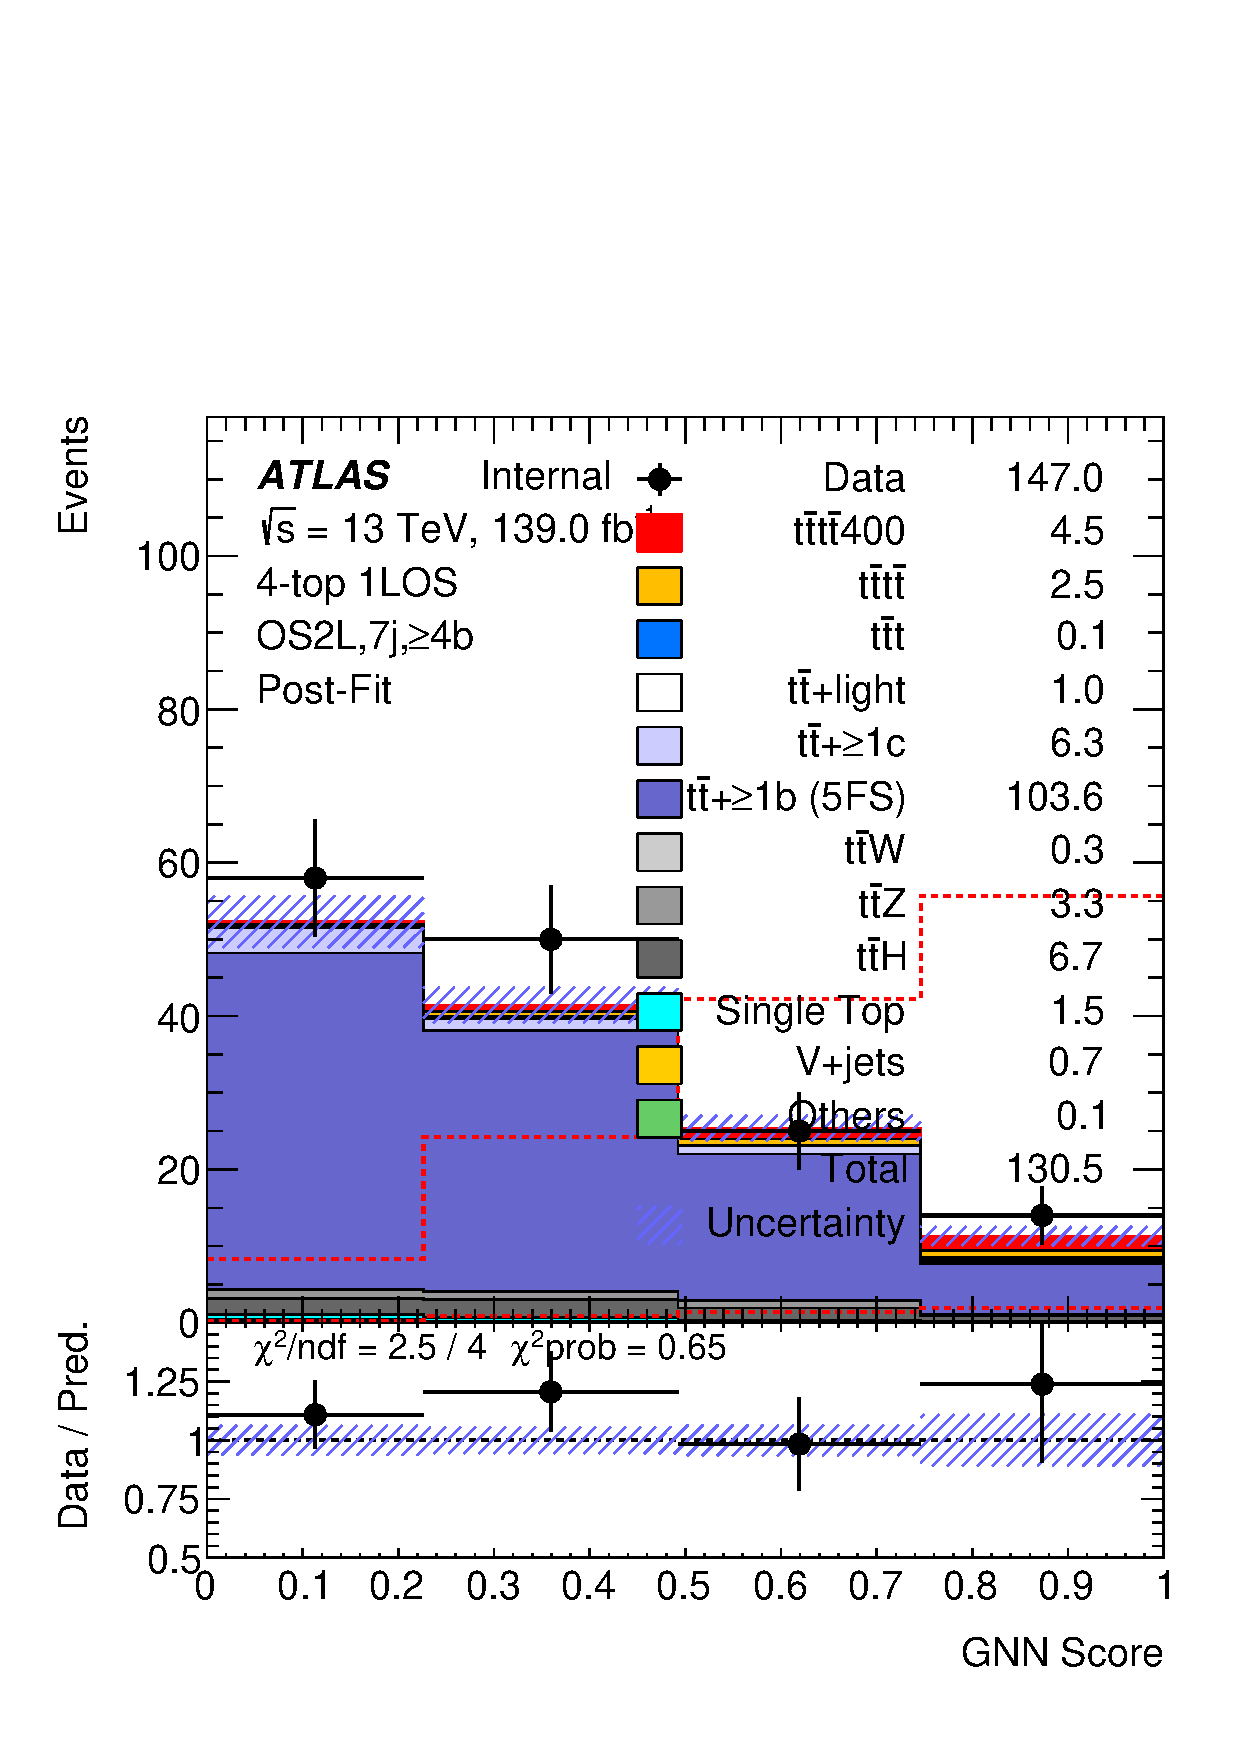
\includegraphics[width=0.31 \textwidth]{figures/fits/GNN/400/all/data_unblindedSplusB/Plots/os2l_7jge4b_postFit.pdf} \\

        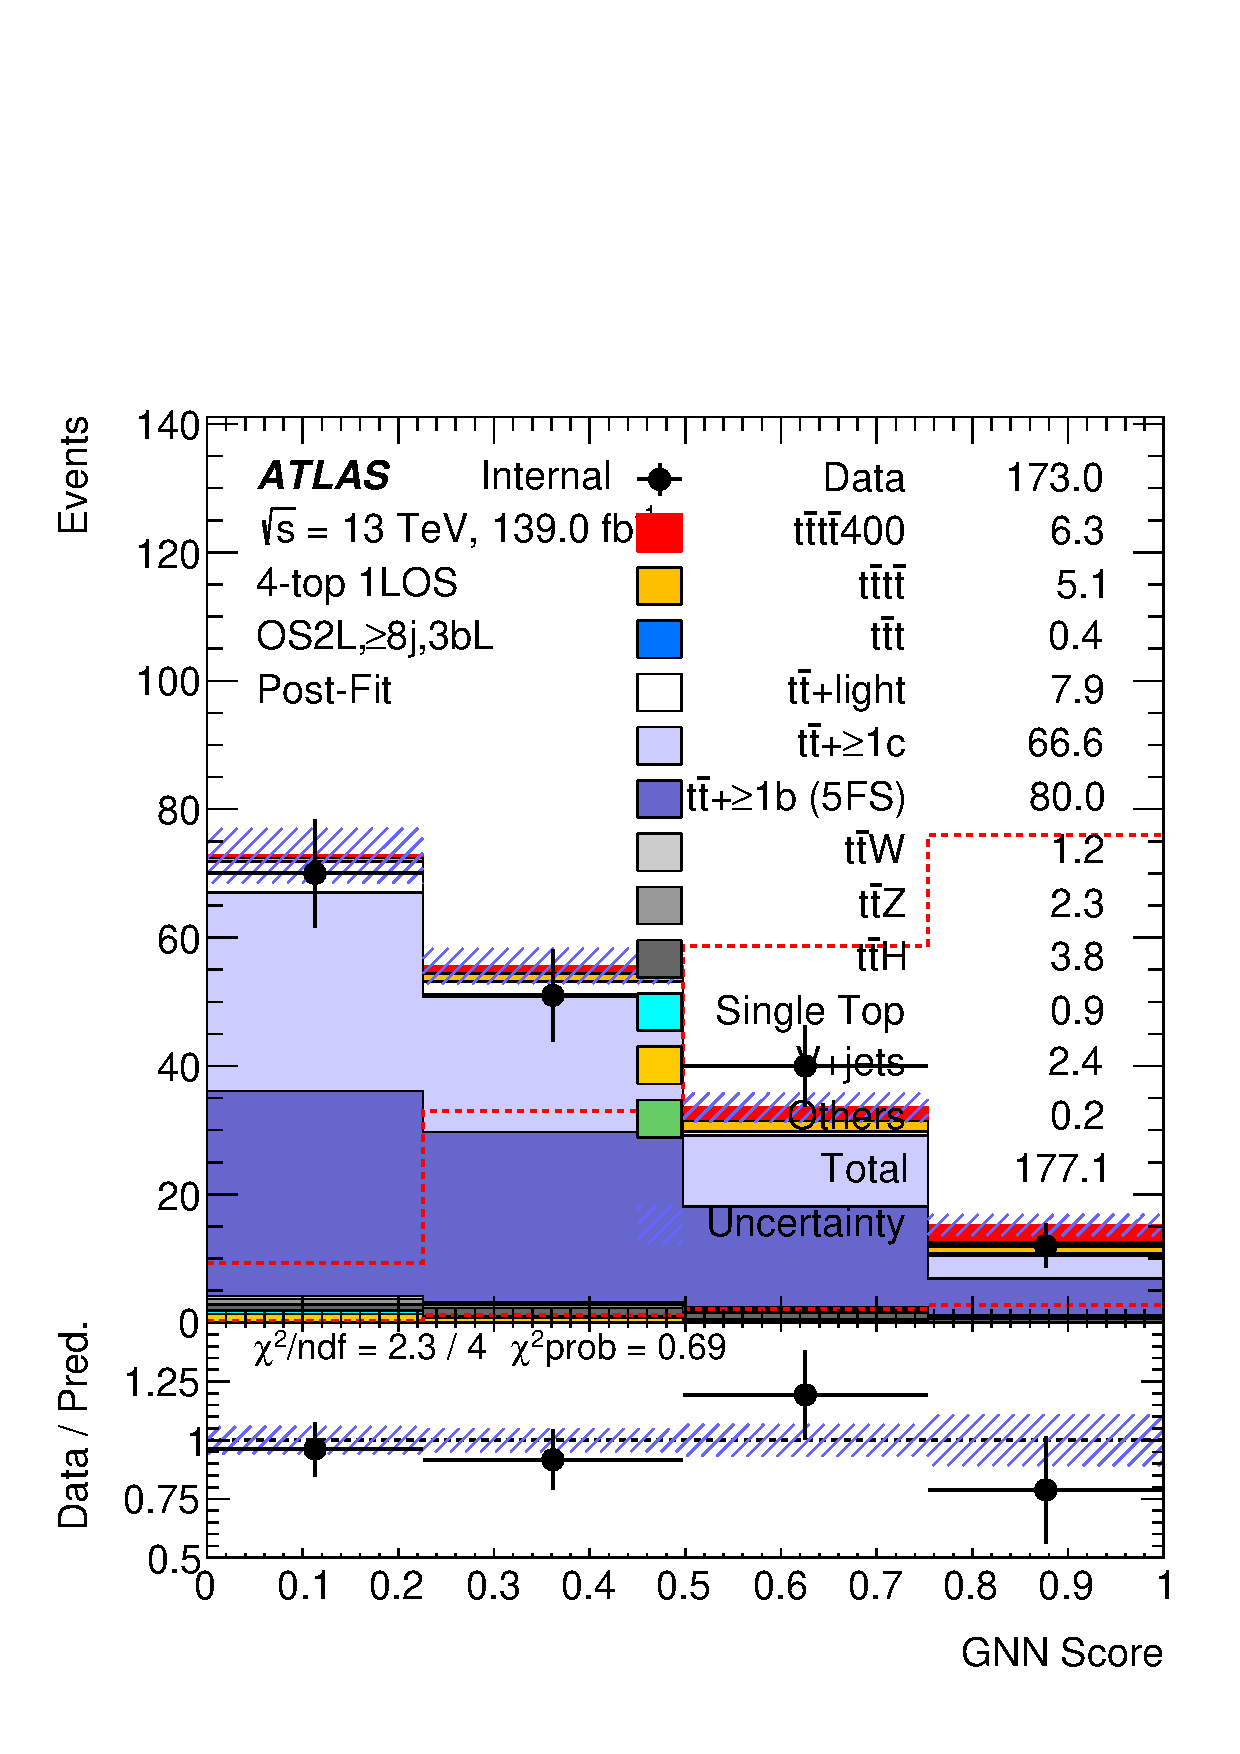
\includegraphics[width=0.31 \textwidth]{figures/fits/GNN/400/all/data_unblindedSplusB/Plots/os2l_ge8j3bL_postFit.pdf} &
        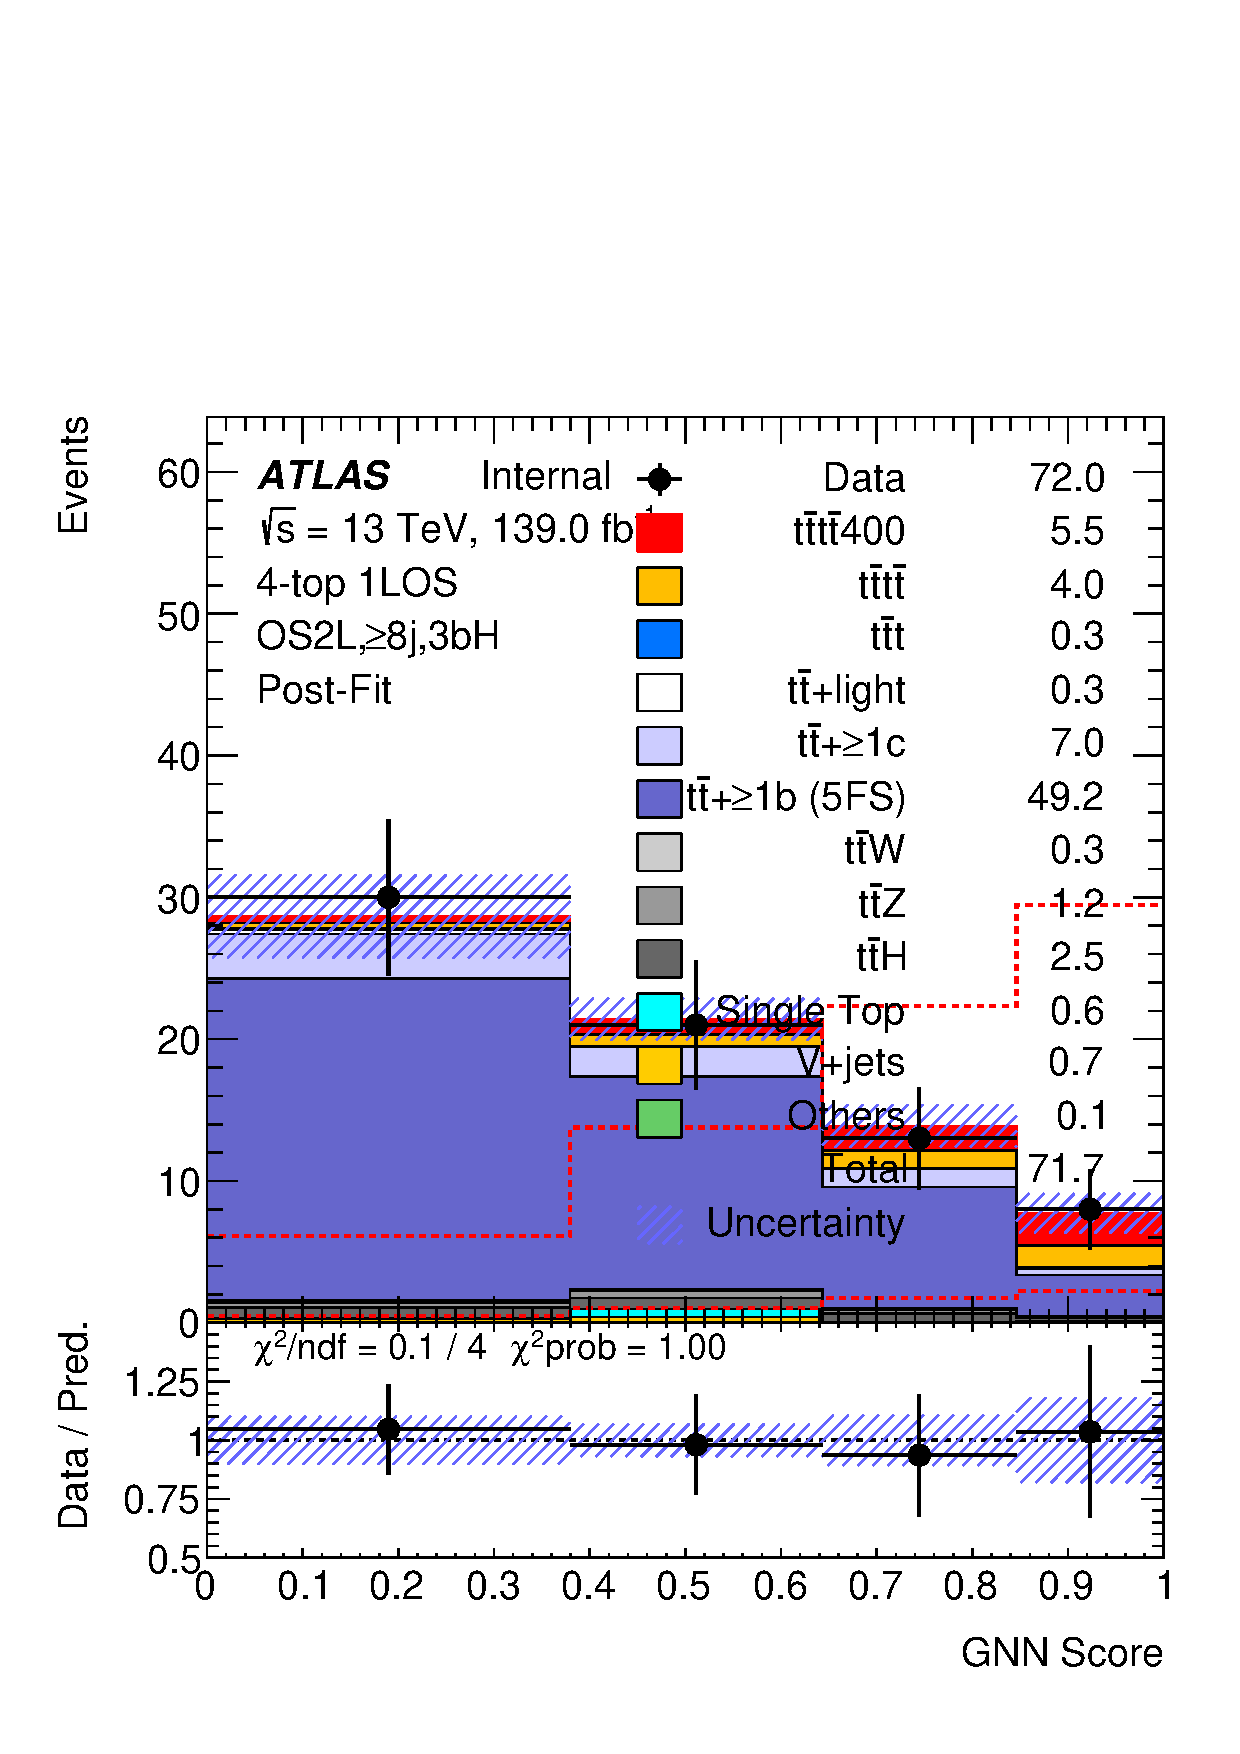
\includegraphics[width=0.31 \textwidth]{figures/fits/GNN/400/all/data_unblindedSplusB/Plots/os2l_ge8j3bH_postFit.pdf} &
        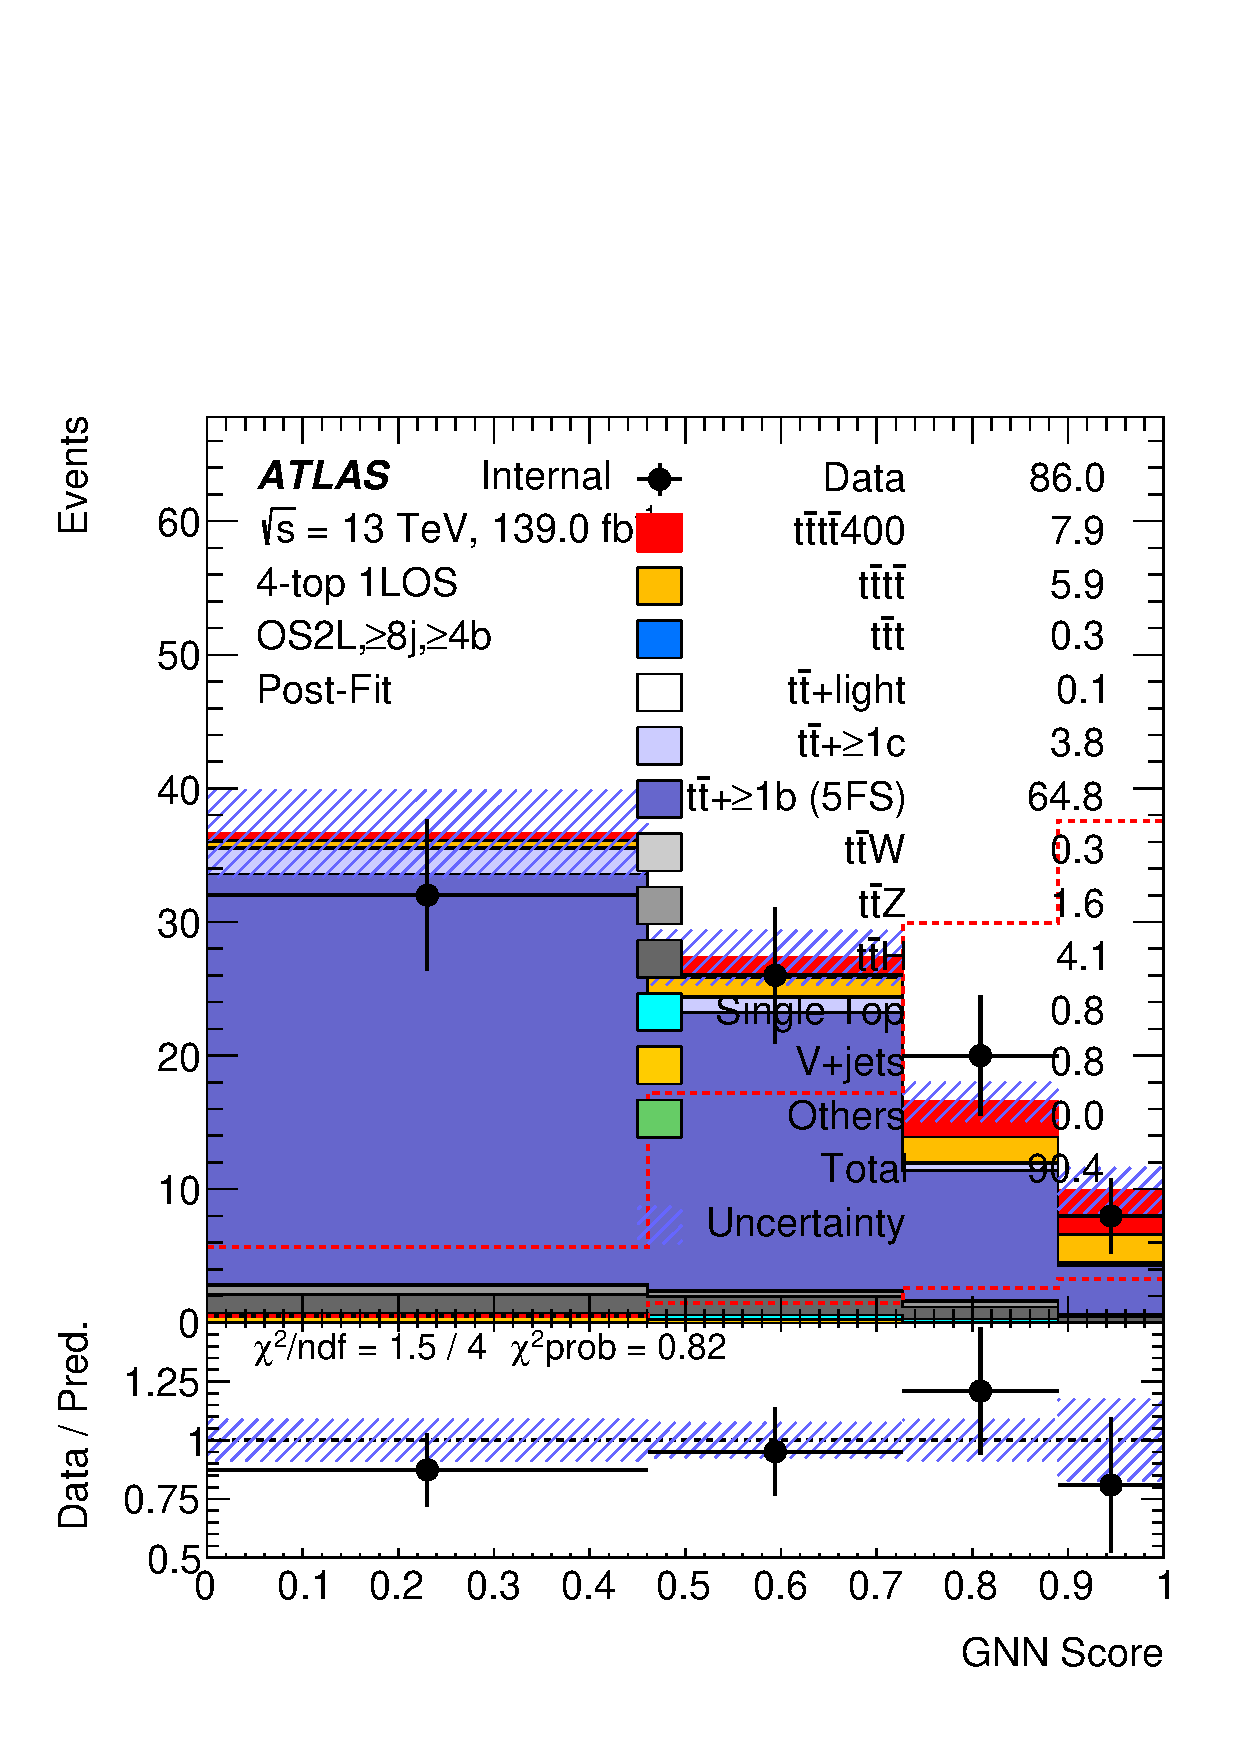
\includegraphics[width=0.31 \textwidth]{figures/fits/GNN/400/all/data_unblindedSplusB/Plots/os2l_ge8jge4b_postFit.pdf} \\
        \end{tabular}
        \caption{\label{fig:unblinded_data_SplusB_postfit_2L}
        Post-fit distributions for the 2LOS regions obtained from the unblinded signal-plus-background data fit at $\boldsymbol{m_H=400}$~GeV. 
        The fit is performed using all regions (1L+2LOS).}
\end{center}
\end{figure}

\subsubsection*{\textbf{Nuisance parameter pulls and correlations}}

The fitted pulls and constraints of nuisance parameters in the combined (1L+2LOS) fit are compared across mass points in Figure~\ref{fig:unblinded_data_SplusB_NP_mass_all}. 
No abnormal constraints or extreme pulls are observed, and the overall behaviour is stable with respect to the assumed signal mass.

\begin{figure}[htbp!]
  \centering
  \begin{subfigure}[t]{0.32\textwidth}
    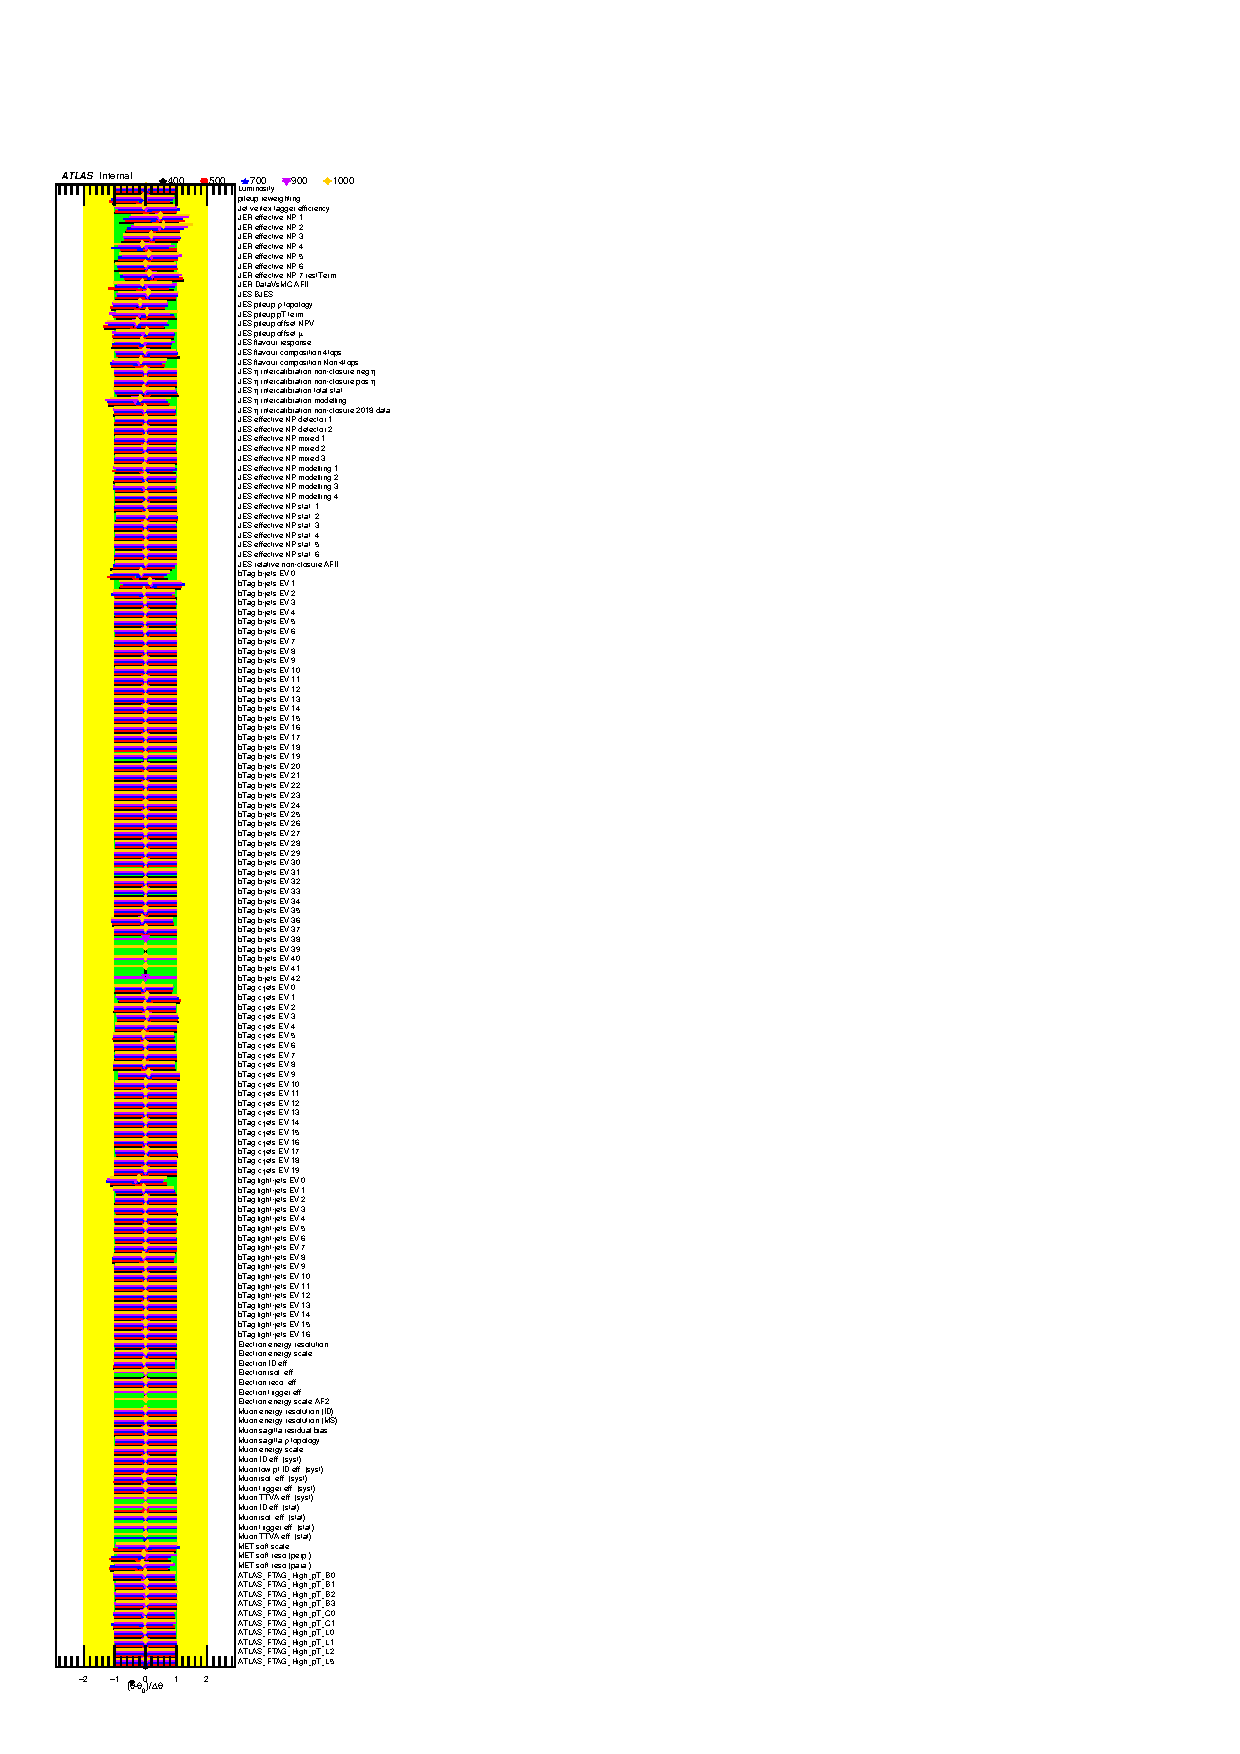
\includegraphics[width=\linewidth]{figures/fits/comparisons/massPoints/GNN/all/data_unblindedSplusB/NuisPar_comp_Instrumental.pdf}
    \subcaption{Instrumental}
    \label{fig:unblinded_data_SplusB_NP_mass_all_instrumental}
  \end{subfigure}
  \begin{subfigure}[t]{0.32\textwidth}
    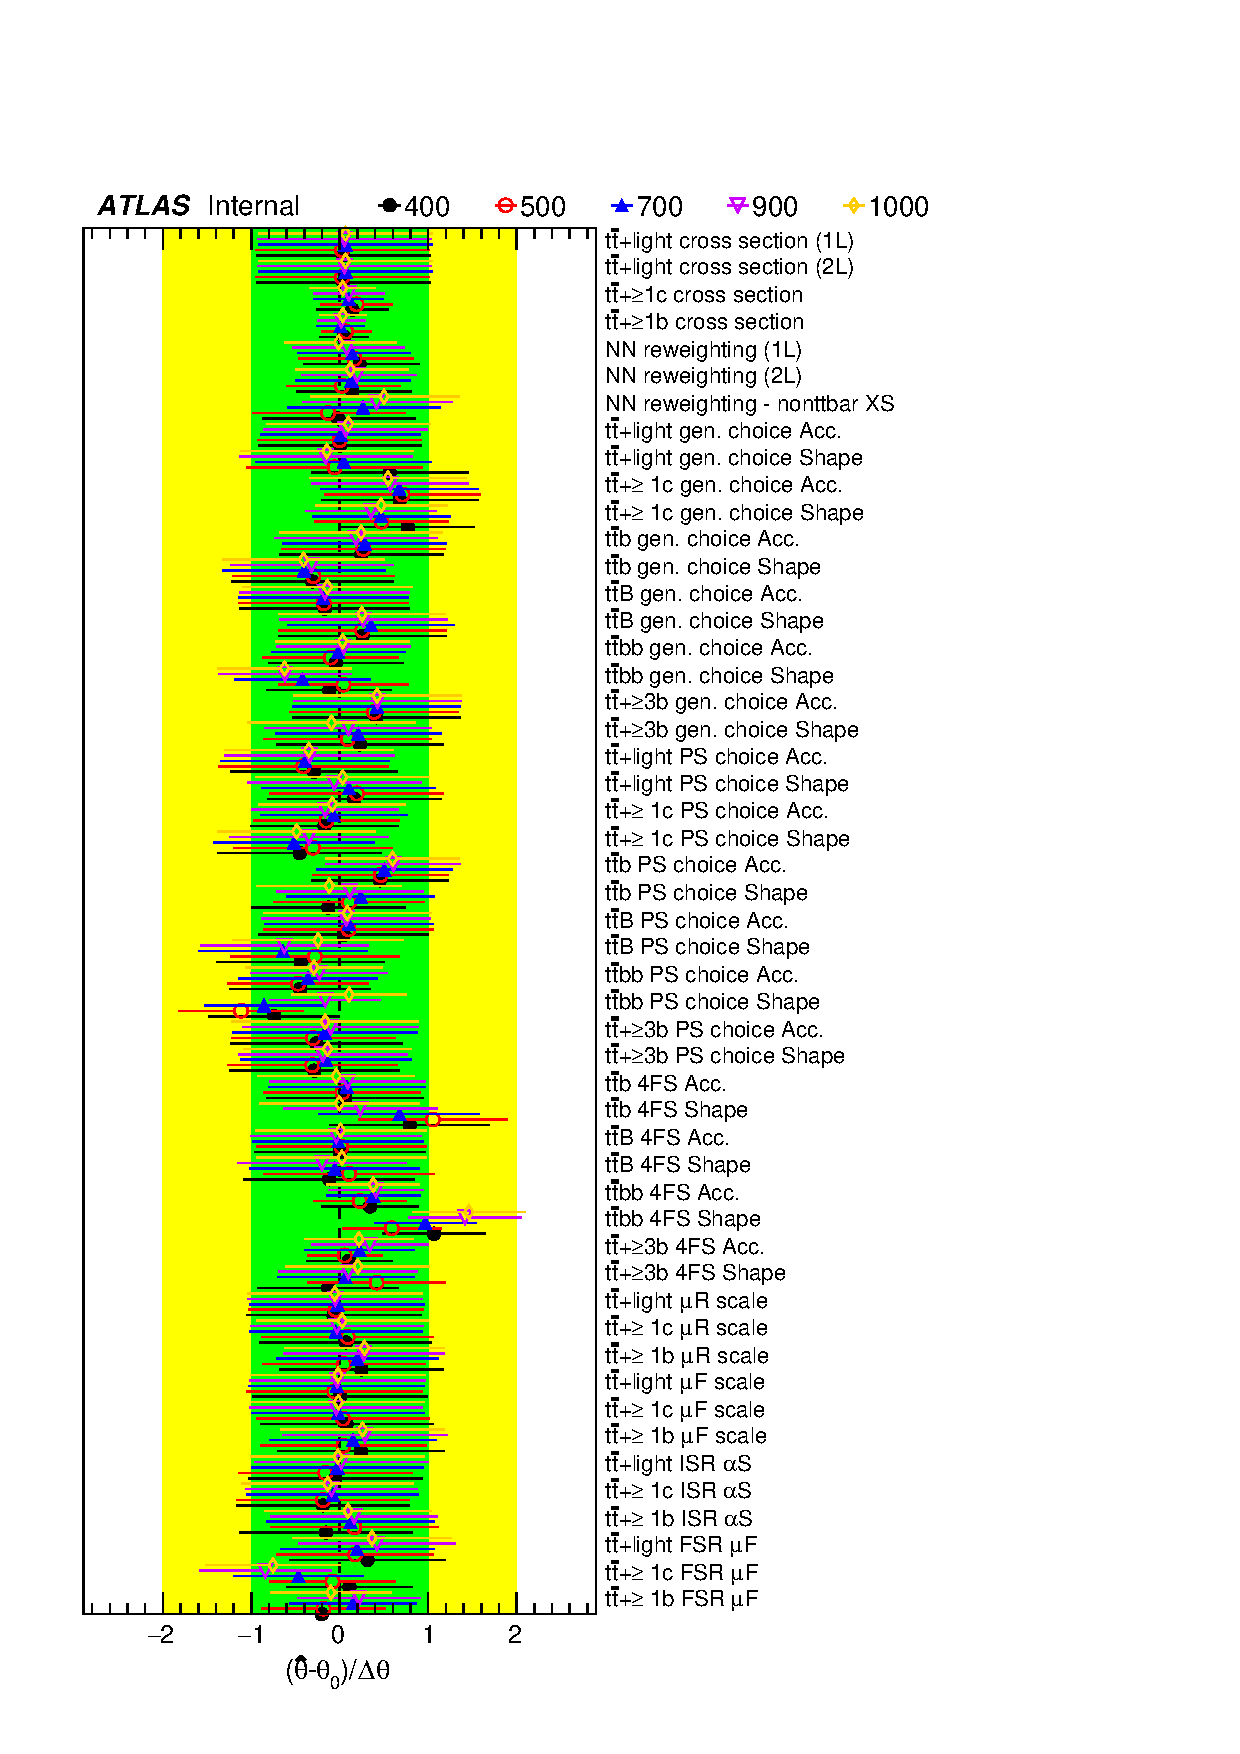
\includegraphics[width=\linewidth]{figures/fits/comparisons/massPoints/GNN/all/data_unblindedSplusB/NuisPar_comp_ttbar.pdf}
    \subcaption{$\boldsymbol{t\bar{t}}$ modelling}
    \label{fig:unblinded_data_SplusB_NP_mass_all_ttbar}
  \end{subfigure}
  \begin{subfigure}[t]{0.32\textwidth}
    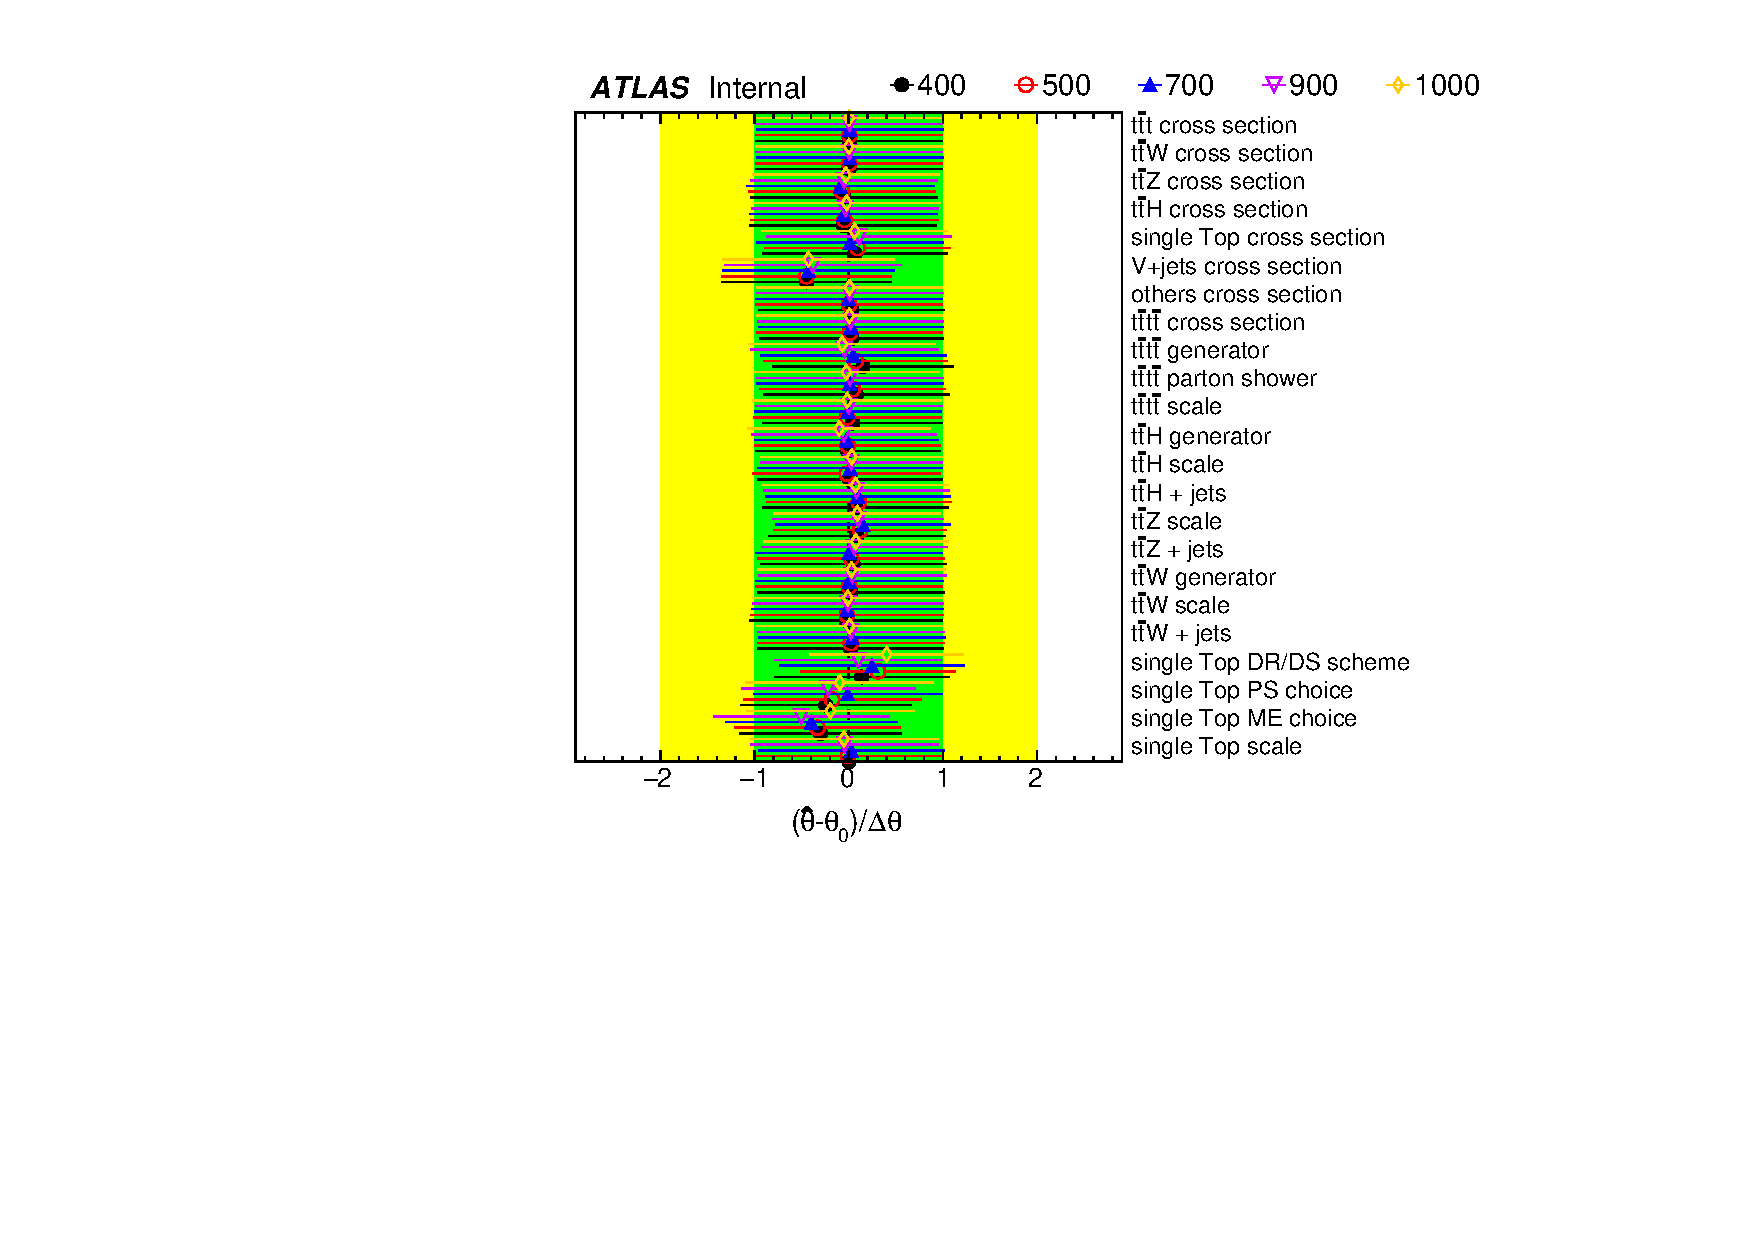
\includegraphics[width=\linewidth]{figures/fits/comparisons/massPoints/GNN/all/data_unblindedSplusB/NuisPar_comp_Other.pdf}
    \subcaption{Other backgrounds}
    \label{fig:unblinded_data_SplusB_NP_mass_all_other}
  \end{subfigure}
  \caption{\label{fig:unblinded_data_SplusB_NP_mass_all}
  Fitted pulls and constraints for nuisance parameters in the combined (1L+2LOS) signal-plus-background unblinded data fit, shown for several mass points.}
\end{figure}

The correlation matrix of the combined S+B fit for $m_H=400$~GeV is shown in Figure~\ref{fig:unblinded_data_SplusB_corr_mH400_Data_all}. 
The correlation structure is consistent with expectations, and correlations with the signal strength parameter are observed for the dominant modelling uncertainties.

\begin{figure}[htbp!]
  \centering
  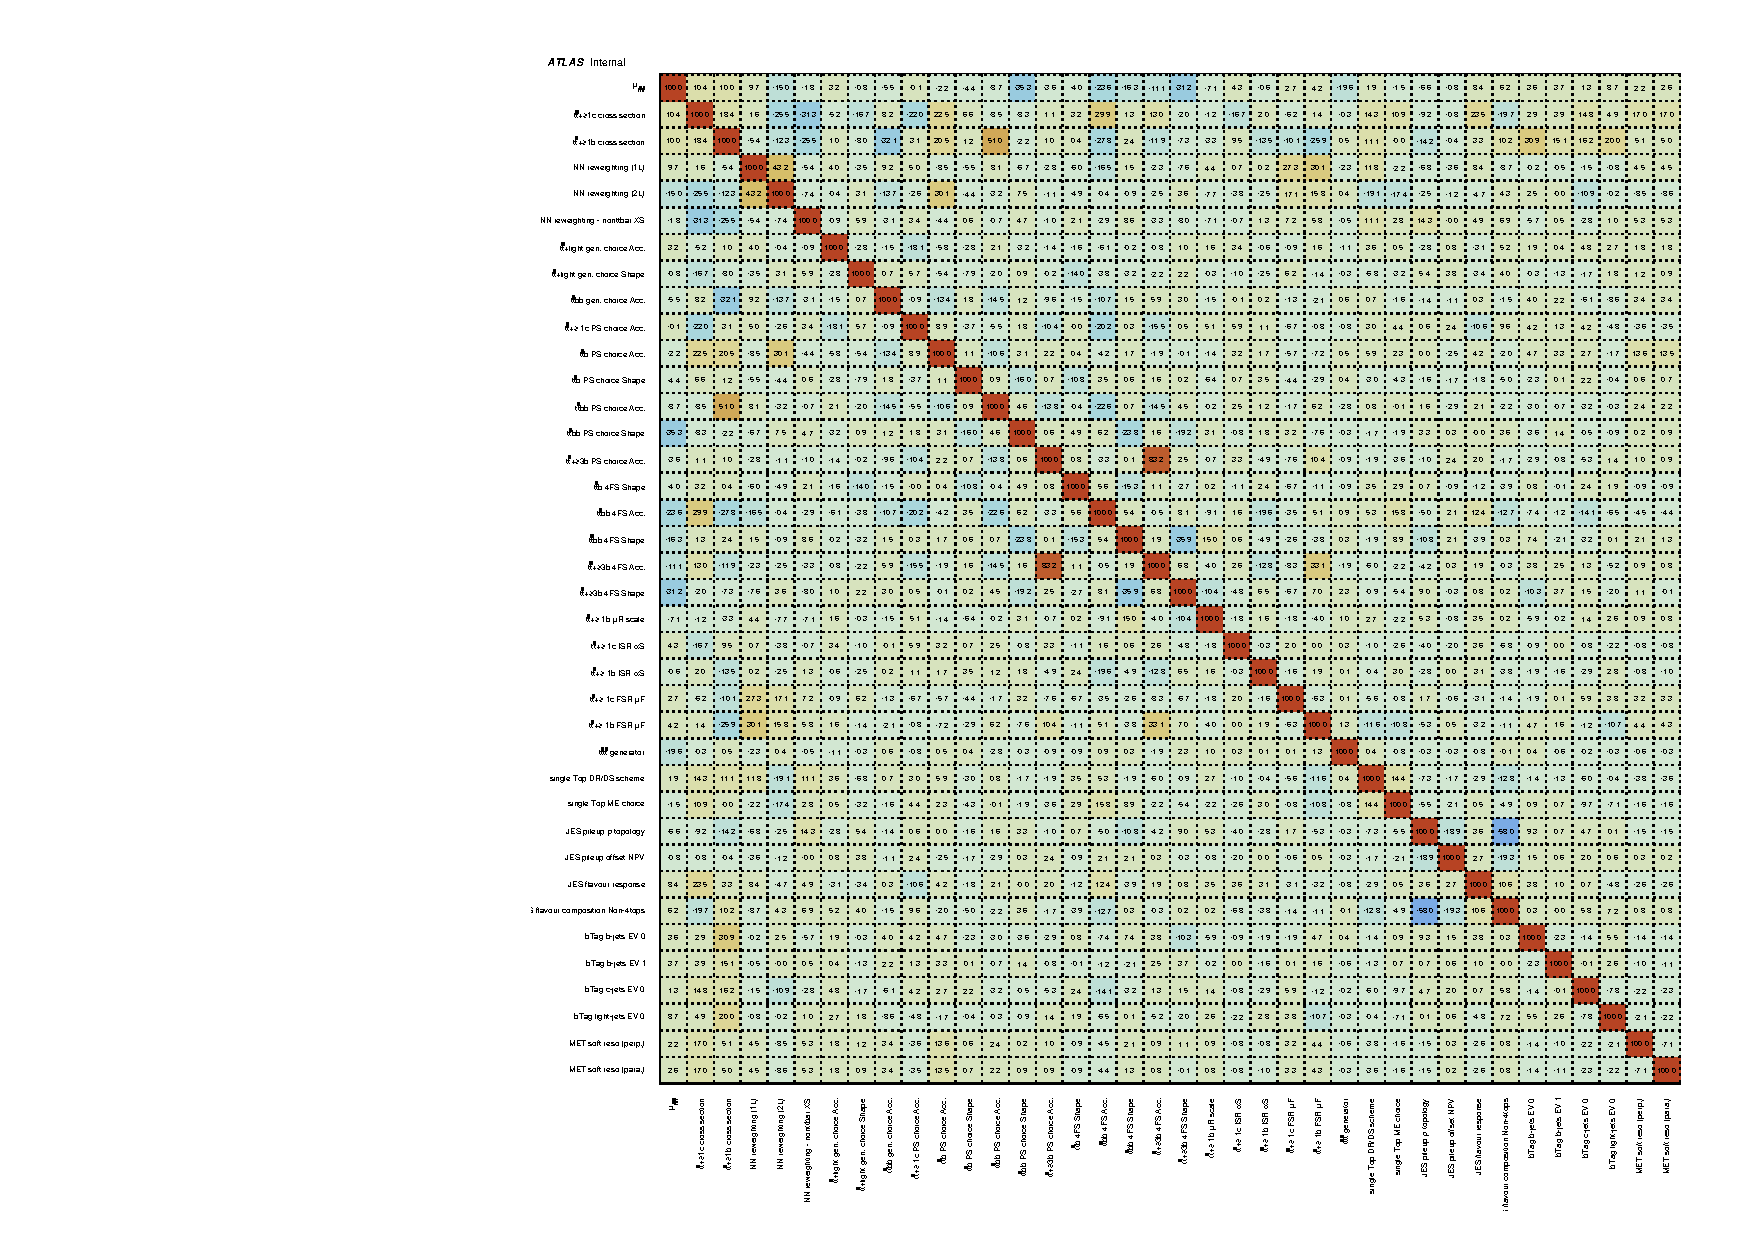
\includegraphics[width=\linewidth]{figures/fits/GNN/400/all/data_unblindedSplusB/CorrMatrix.pdf}
  \caption{\label{fig:unblinded_data_SplusB_corr_mH400_Data_all}
  Correlation matrix of nuisance parameters in the combined signal-plus-background unblinded data fit for $\boldsymbol{m_H=400}$~GeV.}
\end{figure}

\subsubsection*{\textbf{Impact of systematic uncertainties}}

The ranking of nuisance parameters according to their impact on the fitted signal strength is shown in Figures~\ref{fig:Ranking_data_SplusB_400} and~\ref{fig:Ranking_data_SplusB_1000} for $m_H=400$ and $m_H=1000$~GeV, respectively. 
At low masses, the sensitivity is dominated by the modelling of the $t\bar{t}+\geq1b$ background and experimental effects such as jet energy scale and resolution, while at high masses the relative contribution of statistical uncertainties becomes more prominent.

\begin{figure}[htbp!]
  \centering
  \begin{subfigure}[t]{0.49\textwidth}
    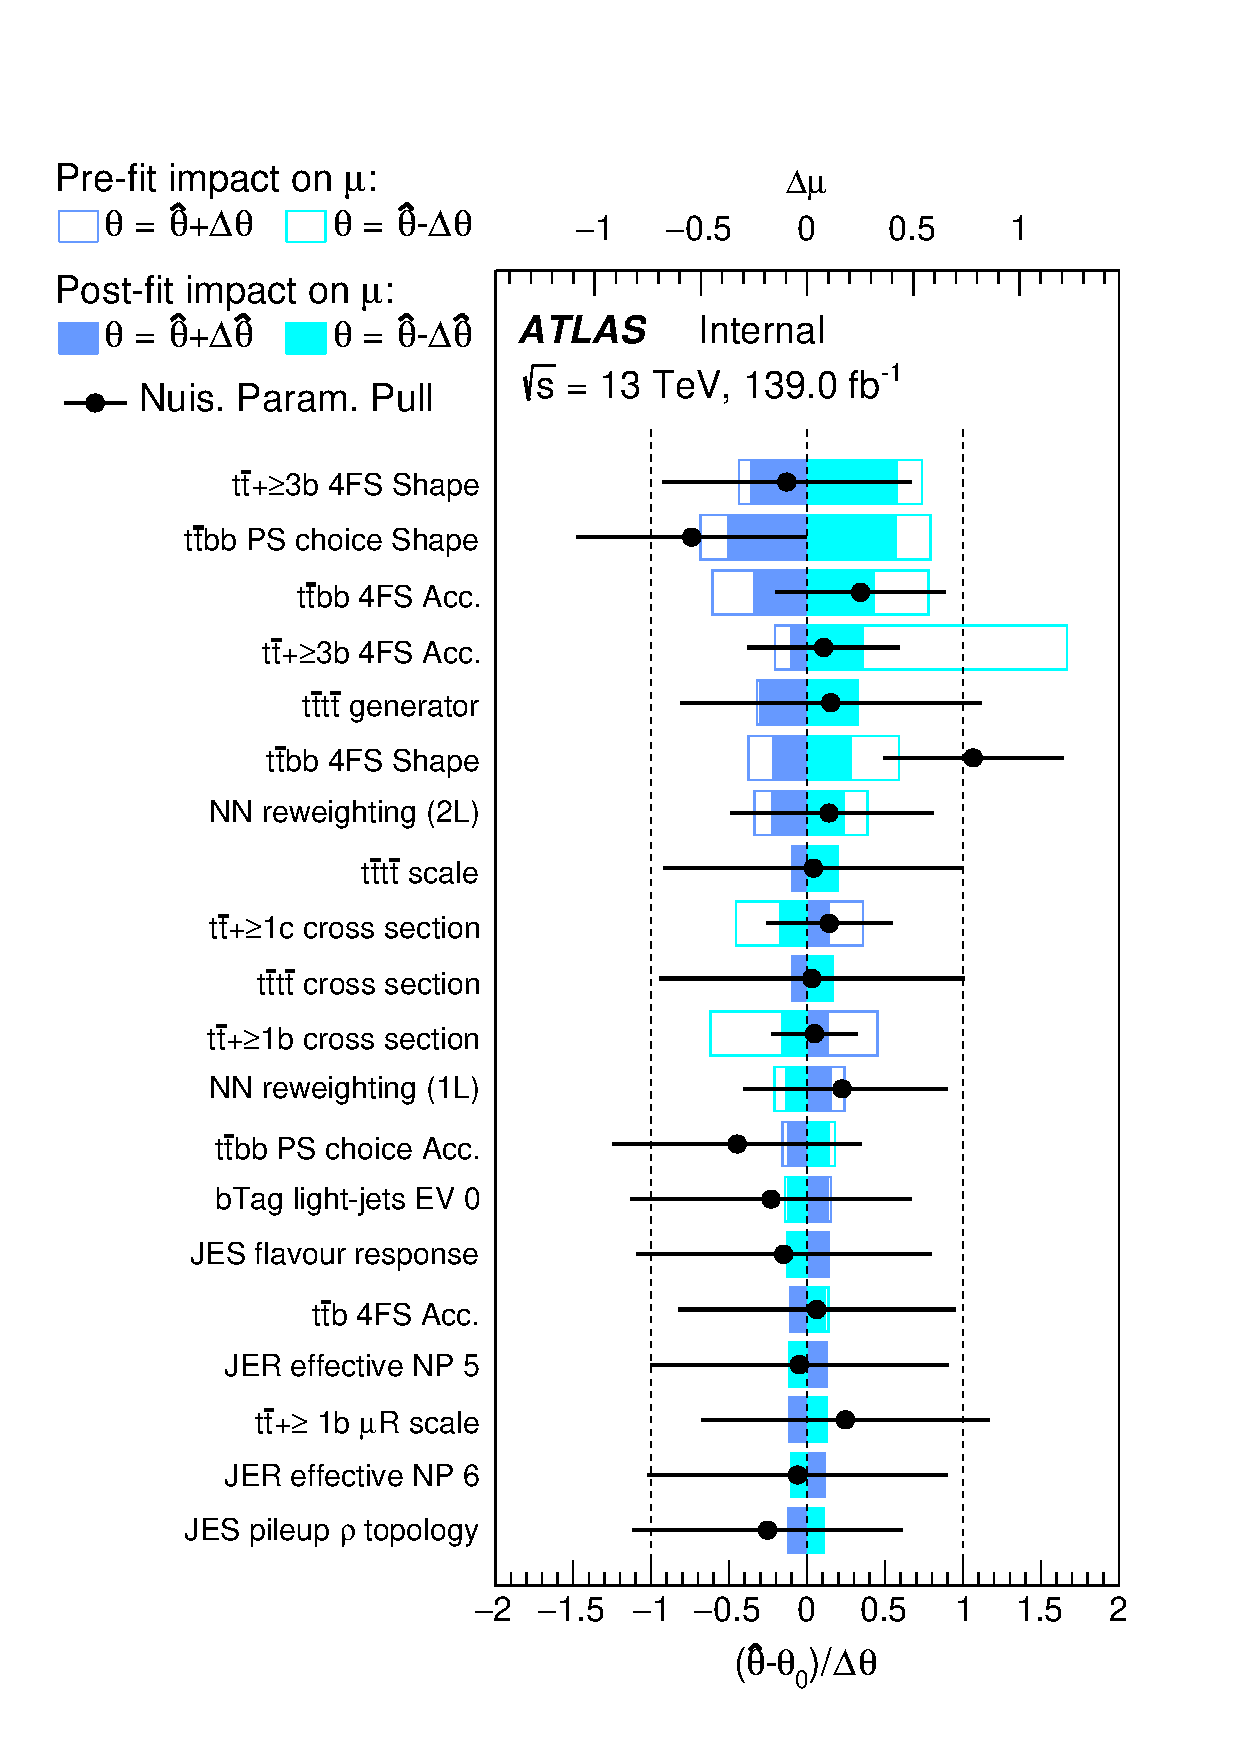
\includegraphics[width=\linewidth]{figures/fits/GNN/400/all/data_unblindedSplusB/Ranking_mu_tttt.pdf}
    \caption{\label{fig:Ranking_data_SplusB_400}$\boldsymbol{m_H=400}$~GeV}
  \end{subfigure}
  \begin{subfigure}[t]{0.49\textwidth}
    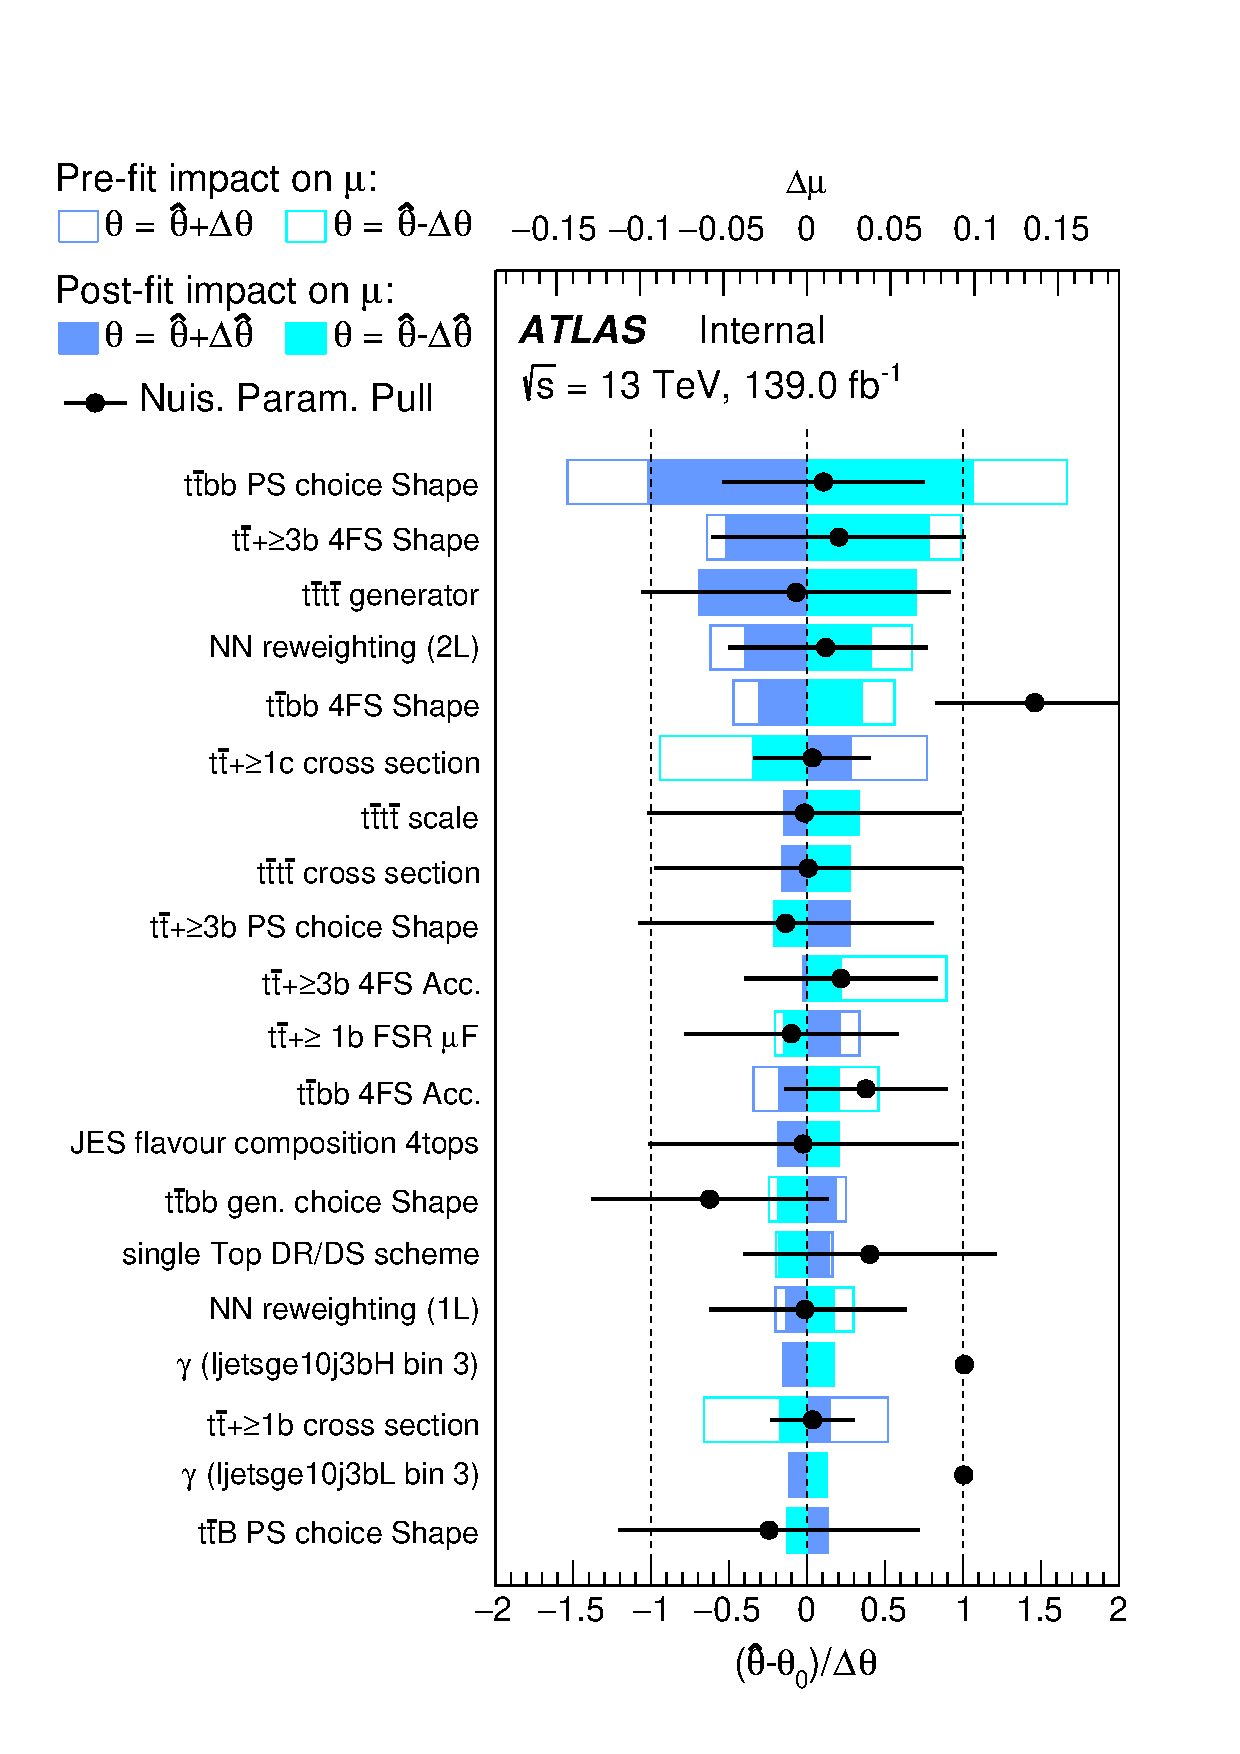
\includegraphics[width=\linewidth]{figures/fits/GNN/1000/all/data_unblindedSplusB/Ranking_mu_tttt.pdf}
    \caption{\label{fig:Ranking_data_SplusB_1000}$\boldsymbol{m_H=1000}$~GeV}
  \end{subfigure}
  \caption{\label{fig:Ranking_data_SplusB}
  Ranking of nuisance parameters according to their impact on the fitted signal strength $\boldsymbol{\mu}$ for two representative mass points in the combined (1L+2LOS) signal-plus-background unblinded data fit.}
\end{figure}

For a quantitative overview, the grouped impacts of nuisance parameters on the extracted cross section are summarised in Table~\ref{tab:grouped_impact_400GeV}. 

\begin{table}[htbp!]
    \begin{center}
    \begin{tabular}{lcc|cc|cc}
    \hline \hline
    Uncertainty source & \multicolumn{6}{c}{$\Delta\sigma_{t\bar{t}H/A(\rightarrow t\bar{t})}$ [fb]} \\
    & \multicolumn{2}{c}{$m_{H/A}$=400 GeV} & \multicolumn{2}{c}{$m_{H/A}$=700 GeV} & \multicolumn{2}{c}{$m_{H/A}$=1000 GeV} \\
    \hline
    \textbf{Signal Modelling} & & & & & & \\
    BSM $t\bar{t}t\bar{t}$ modelling & \multicolumn{2}{c}{$\textless 1$} & +0.1 & $\textless 0.1$ & \multicolumn{2}{c}{$\textless 0.1$} \\
    \hline
    \textbf{Background Modelling} & & & & & & \\
    $t\bar{t}+\geq1b$ modelling & +11 & -10 & +3.7 & -3.4 & +1.9 & -1.7 \\
    $t\bar{t}$+jets reweighting & +3 & -3 & +1.0 & -1.0 & +0.5 & -0.5 \\
    Other background modelling & +3 & -3 & +2.1 & -2.2 & +0.9 & -0.9 \\
    $t\bar{t}+\geq1c$ modelling & +2 & -2 & +0.9 & -0.8 & +0.4 & -0.4 \\
    $t\bar{t}$+light modelling & +1 & -1 & +0.2 & -0.2 & \multicolumn{2}{c}{$\textless 0.1$} \\
    \hline
    \textbf{Experimental} & & & & & & \\
    Jet energy scale and resolution & +4 & -2 & +1.3 & -0.8 & +0.5 & -0.3 \\
    MC statistical uncertainties & +2 & -2 & +0.6 & -0.6 & +0.4 & -0.4 \\
    b-tagging efficiency and high-pT extrapolation & +2 & -1 & +0.7 & -0.4 & +0.3 & -0.1 \\
    Luminosity & \multicolumn{2}{c}{$\textless 1$} & +0.3 & -0.1 & \multicolumn{2}{c}{$\textless 0.1$} \\
    Other uncertainties & \multicolumn{2}{c}{$\textless 1$} & +0.3 & -0.5 & +0.1 & -0.2 \\
    \hline \hline
    \textbf{Total systematic uncertainty} & +13 & -12 & +4.8 & -4.6 & +2.5 & -2.4 \\
    \hline \hline
    \textbf{Statistical uncertainty} & +6 & -6 & +3.3 & -3.2 & +2.3 & -2.2 \\
    \hline \hline
    \textbf{Total uncertainty} & +14 & -13 & +5.6 & -5.4 & +3.2 & -3.0 \\
    \hline \hline
    \end{tabular}
    \caption{\label{tab:grouped_impact_400GeV}
    Grouped impact of nuisance parameters on the extracted cross section for three representative mass points.}
    \end{center}
\end{table}

\subsubsection*{\textbf{Signal strength and significance}}

The fitted signal strength $\mu$ as a function of $m_{H/A}$ is shown in Figure~\ref{fig:data_SplusB_signal_strength}. 
The results are consistent with the background-only hypothesis within uncertainties across the full mass range. 
The observed and expected significances are shown in Figure~\ref{fig:data_SplusB_significance}, and no statistically significant excess is observed.

\begin{figure}[htbp!]
  \centering
  \begin{subfigure}[t]{0.49\textwidth}
    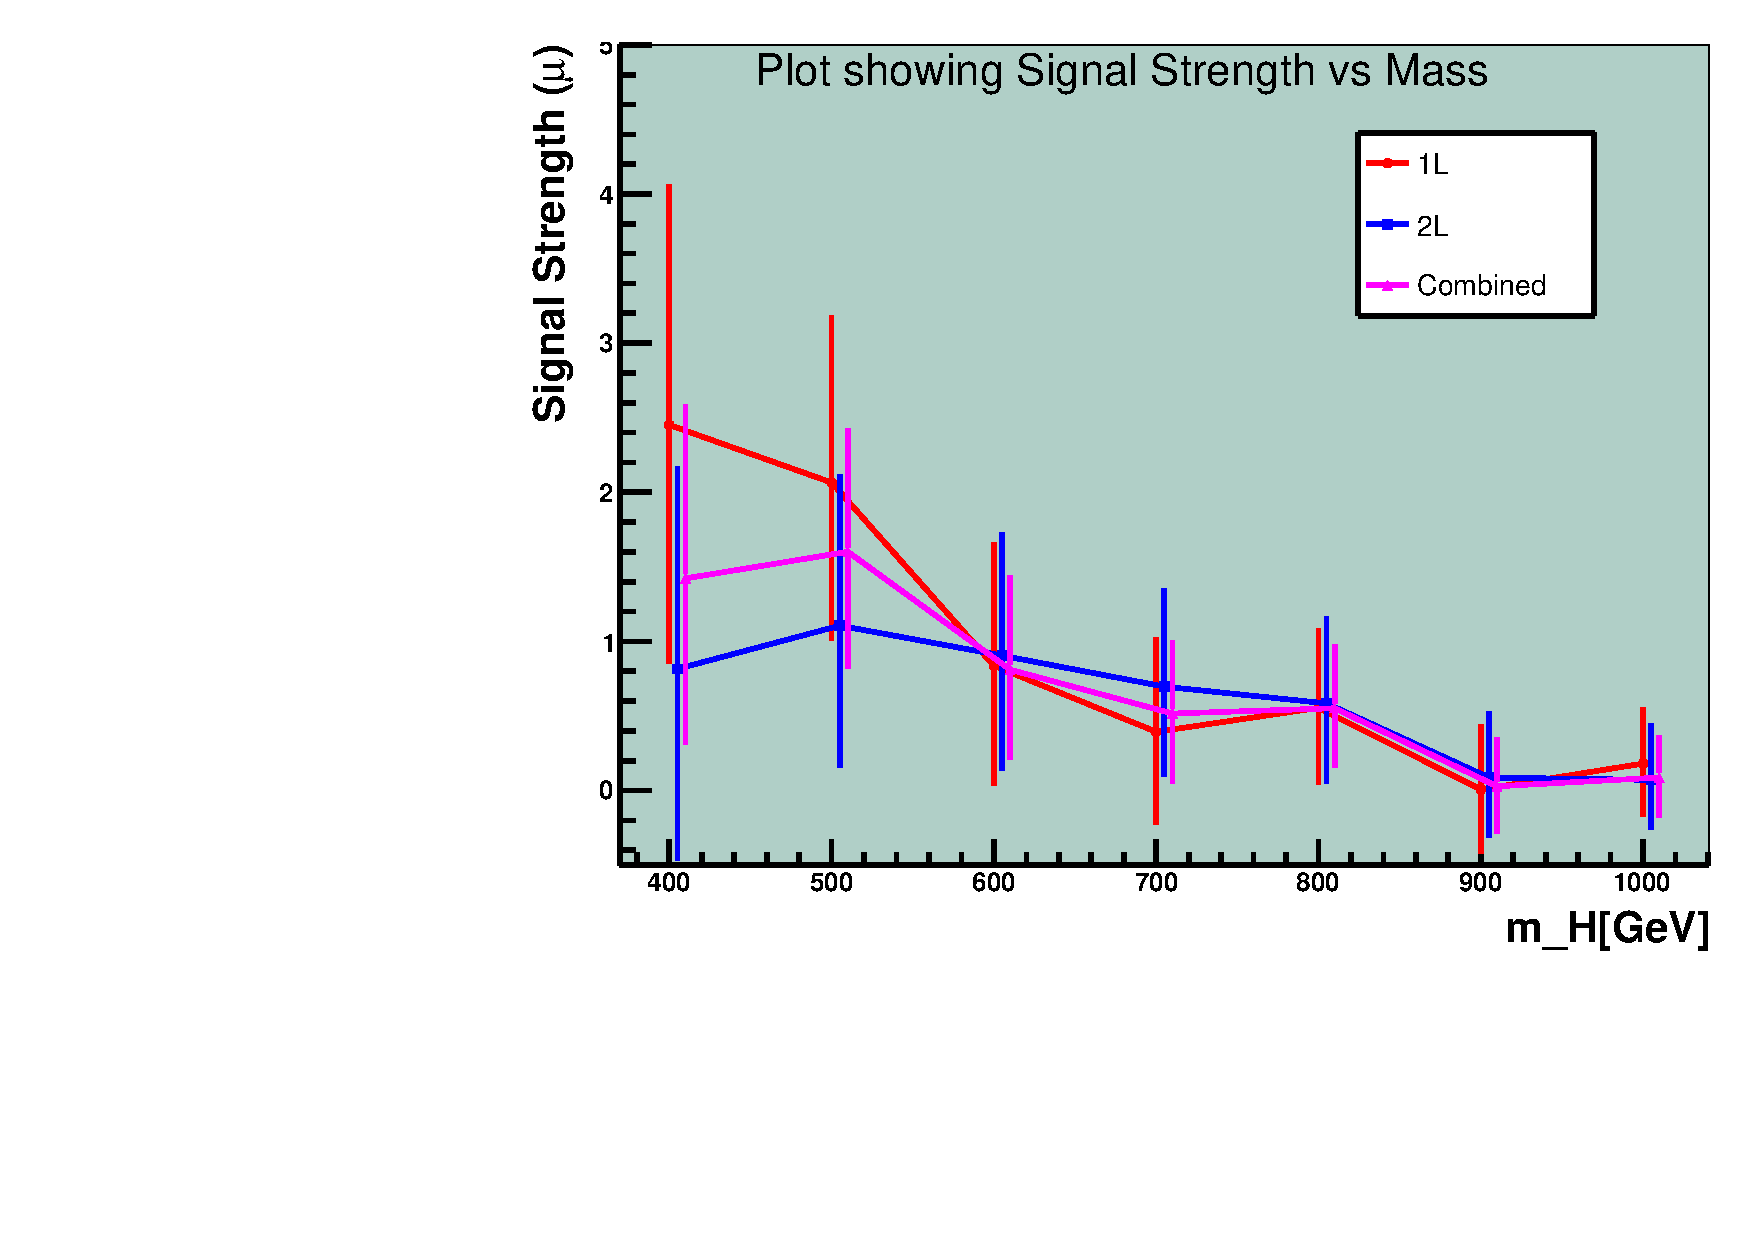
\includegraphics[width=\linewidth]{figures/fits/signalStrengthVsMass.pdf}
    \subcaption{\label{fig:data_SplusB_signal_strength}
    Fitted signal strength $\boldsymbol{\mu}$ as a function of the heavy Higgs boson mass.}
  \end{subfigure}
  \hfill
  \begin{subfigure}[t]{0.49\textwidth}
    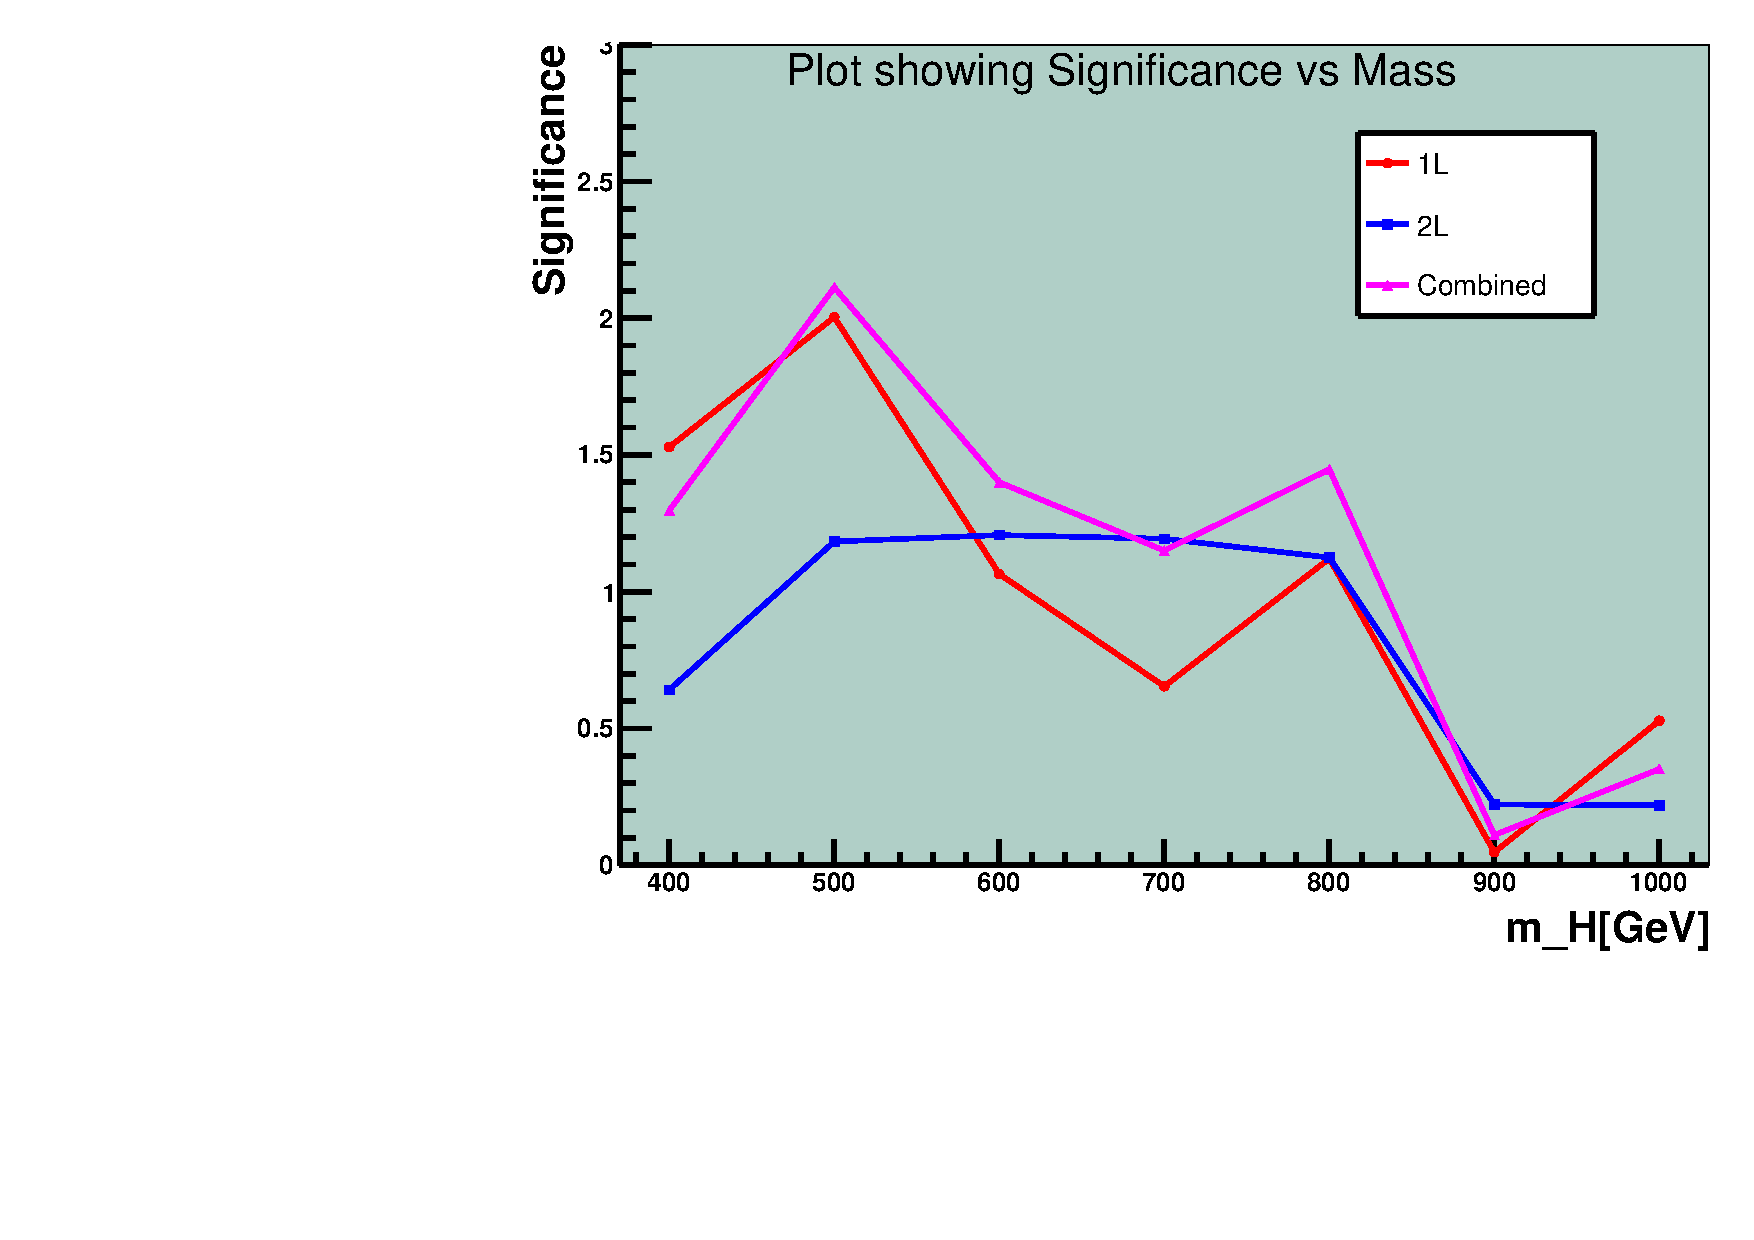
\includegraphics[width=\linewidth]{figures/fits/significanceVsMass.pdf}
    \subcaption{\label{fig:data_SplusB_significance}
    Observed and expected significances as a function of the heavy Higgs boson mass.}
  \end{subfigure}
  \caption{\label{fig:data_SplusB_results}
  Summary of the signal-plus-background fit results as a function of $\boldsymbol{m_{H/A}}$.
  Left: fitted signal strength $\boldsymbol{\mu}$. 
  Right: observed and expected significances.}
\end{figure}

\subsection{Interpretation in the 2HDM framework}
\label{sec:limits_data}

The results of the signal-plus-background fit are interpreted in the context of the two-Higgs-doublet model (2HDM) of type-II. 
In this framework, a heavy neutral scalar $H$ or pseudoscalar $A$ can be produced in association with a top-quark pair and subsequently decay into $t\bar{t}$, leading to a $t\bar{t}t\bar{t}$ final state.

Upper limits at 95\% confidence level (CL) are derived on the production cross section times branching fraction,
\[
\sigma(pp \to t\bar{t}H/A) \times \mathcal{B}(H/A \to t\bar{t}),
\]
as a function of the heavy Higgs boson mass $m_{H/A}$. 
The limits are computed using the CL$_\mathrm{s}$ prescription described in Section~\ref{sec:likelihood_construction}.

\subsubsection{Interpretation of the 1L/2LOS channel}
\label{sec:limits_1LOS}

The expected and observed limits obtained from the 1L/2LOS analysis are shown in Figure~\ref{fig:limits_1LOS}. 
The observed limits decrease from approximately 15~fb at $m_{H/A}=400$~GeV to about 5~fb at $m_{H/A}=1000$~GeV and are consistent with the background-only hypothesis across the full mass range considered.

\begin{figure}[htbp!]
  \centering
  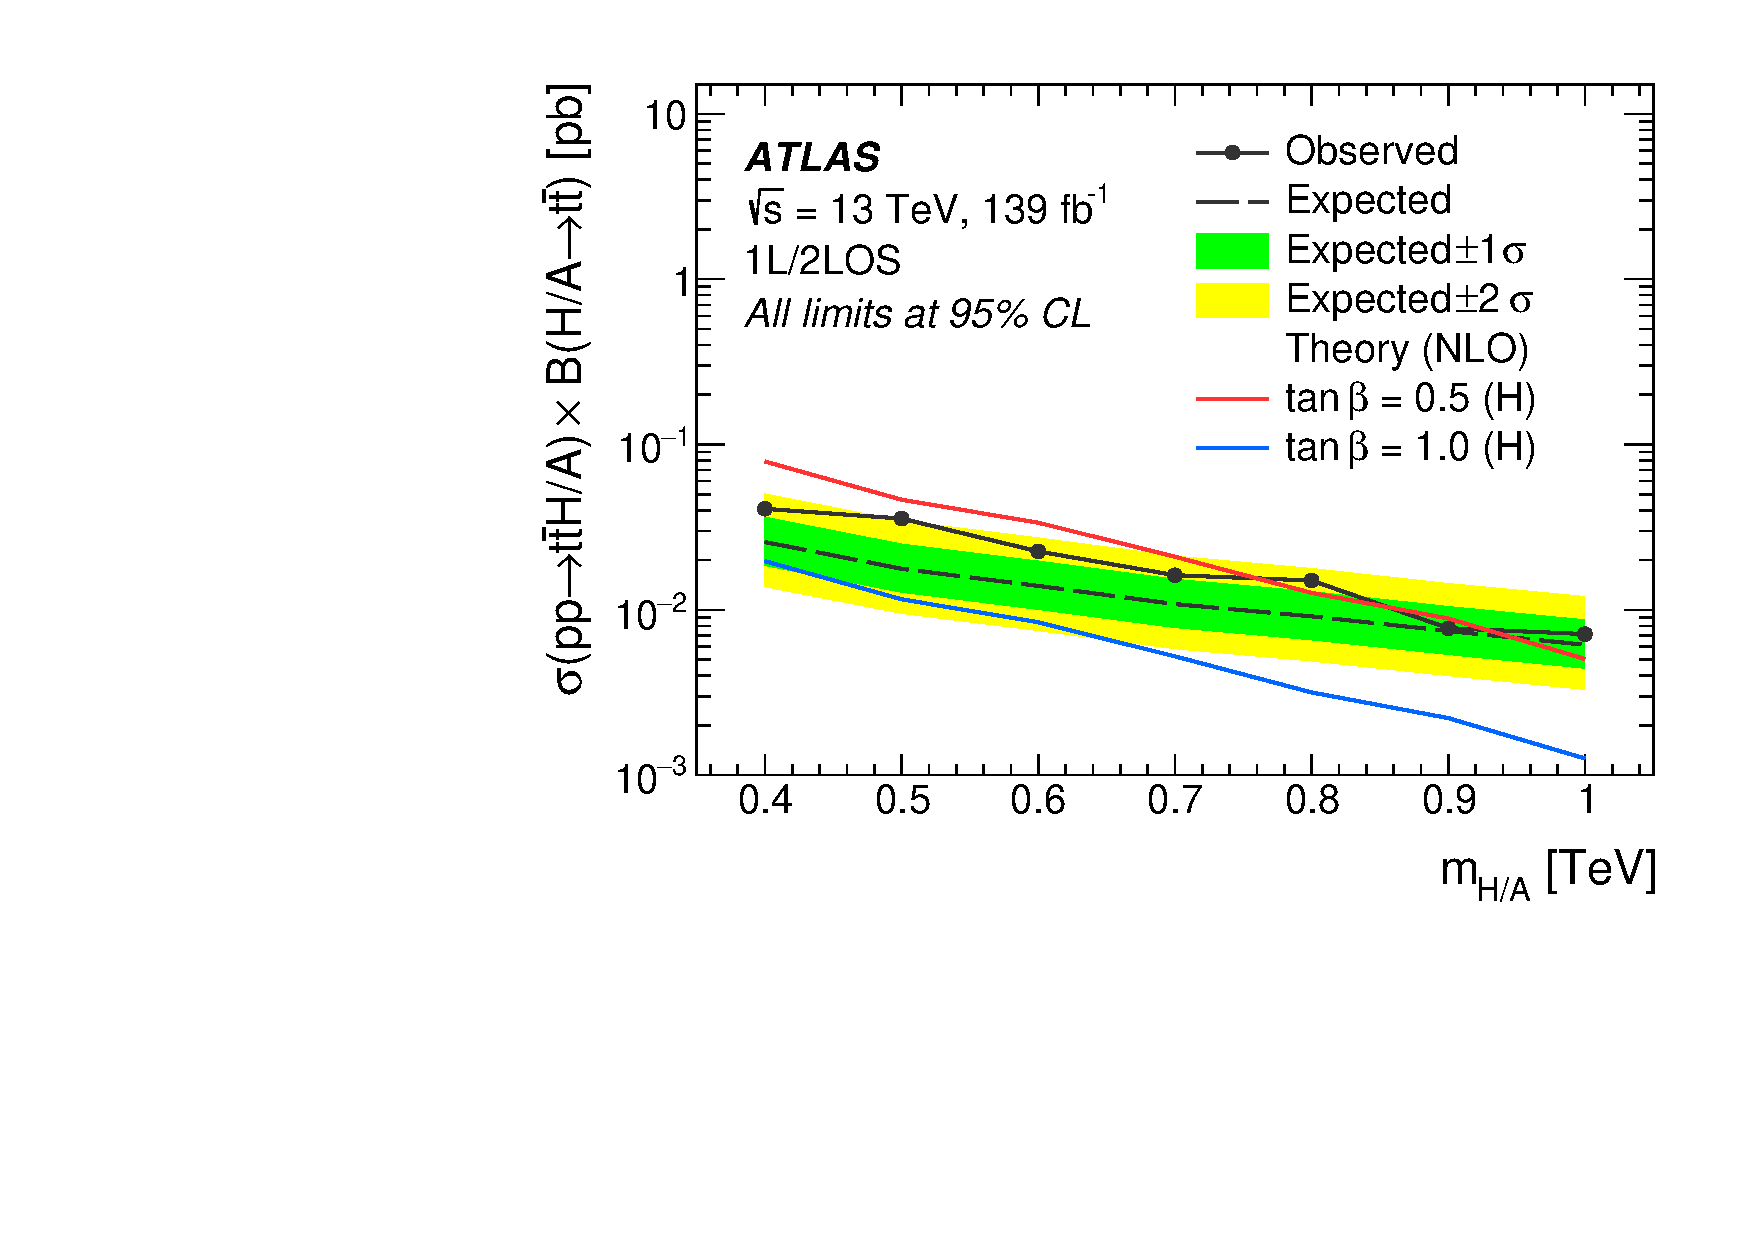
\includegraphics[width=0.6\textwidth]{figures/figures_paper/limit_1LOS_only.pdf}
  \caption{
  Expected and observed 95\% CL upper limits on 
  $\boldsymbol{\sigma(pp \to t\bar{t}H/A) \times \mathcal{B}(H/A \to t\bar{t})}$ 
  as a function of $\boldsymbol{m_{H/A}}$ for the 1L/2LOS analysis.}
  \label{fig:limits_1LOS}
\end{figure}

These limits are translated into exclusion regions in the $(m_{H/A}, \tan\beta)$ parameter plane of the 2HDM type-II. 
Figure~\ref{fig:2D_1LOS} shows the observed and expected exclusions for three benchmark scenarios:
(i) $m_H = m_A$ with both states contributing,
(ii) only the scalar $H$, and
(iii) only the pseudoscalar $A$ contributing to the final state.

\begin{figure}[htbp!]
  \centering
  \begin{subfigure}[t]{0.49\textwidth}
    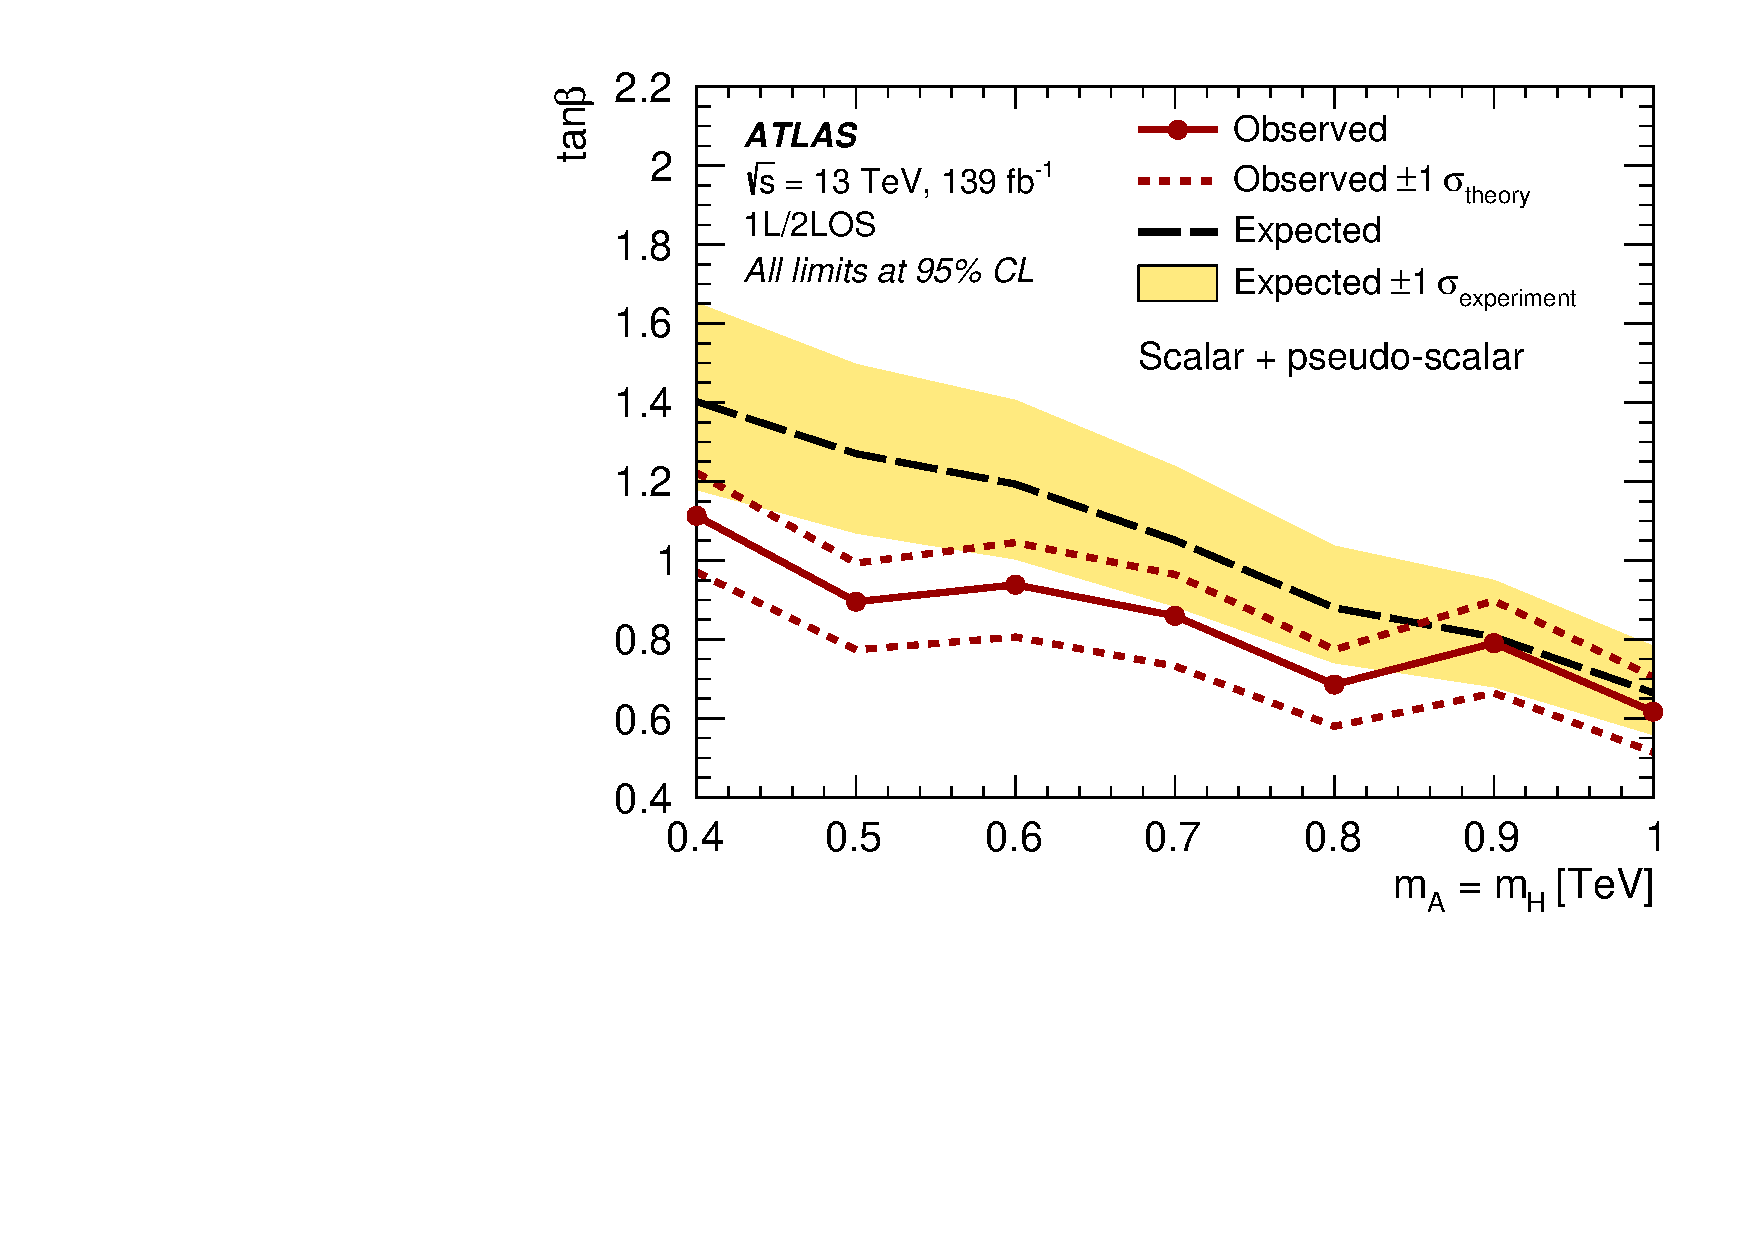
\includegraphics[width=\linewidth]{figures/figures_paper/Data_12fb_All_1LOS.pdf}
    \caption{$m_H = m_A$, both contribute}
  \end{subfigure}
  \hfill
  \begin{subfigure}[t]{0.49\textwidth}
    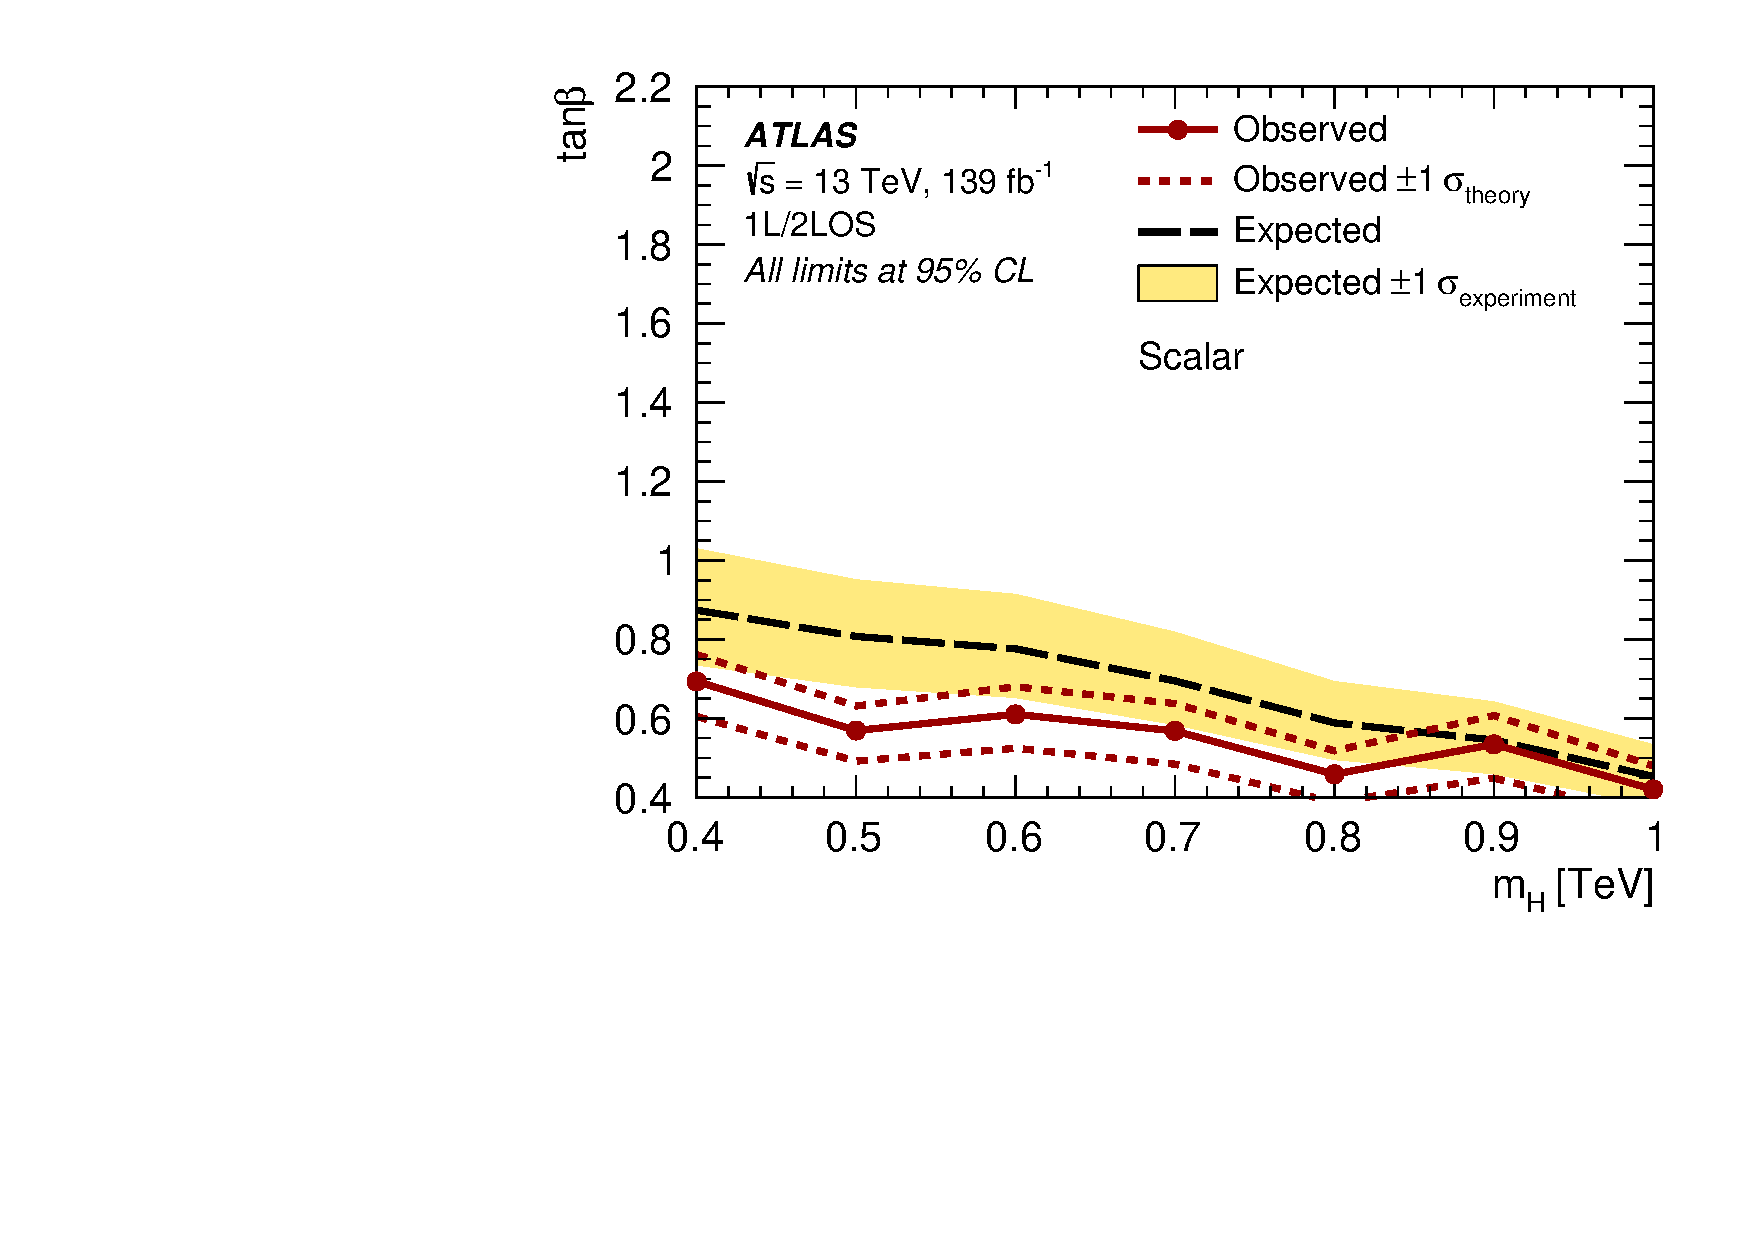
\includegraphics[width=\linewidth]{figures/figures_paper/Data_12fb_ttH_1LOS.pdf}
    \caption{Scalar $H$ only}
  \end{subfigure}

  \vspace{0.4cm}

  \begin{subfigure}[t]{0.49\textwidth}
    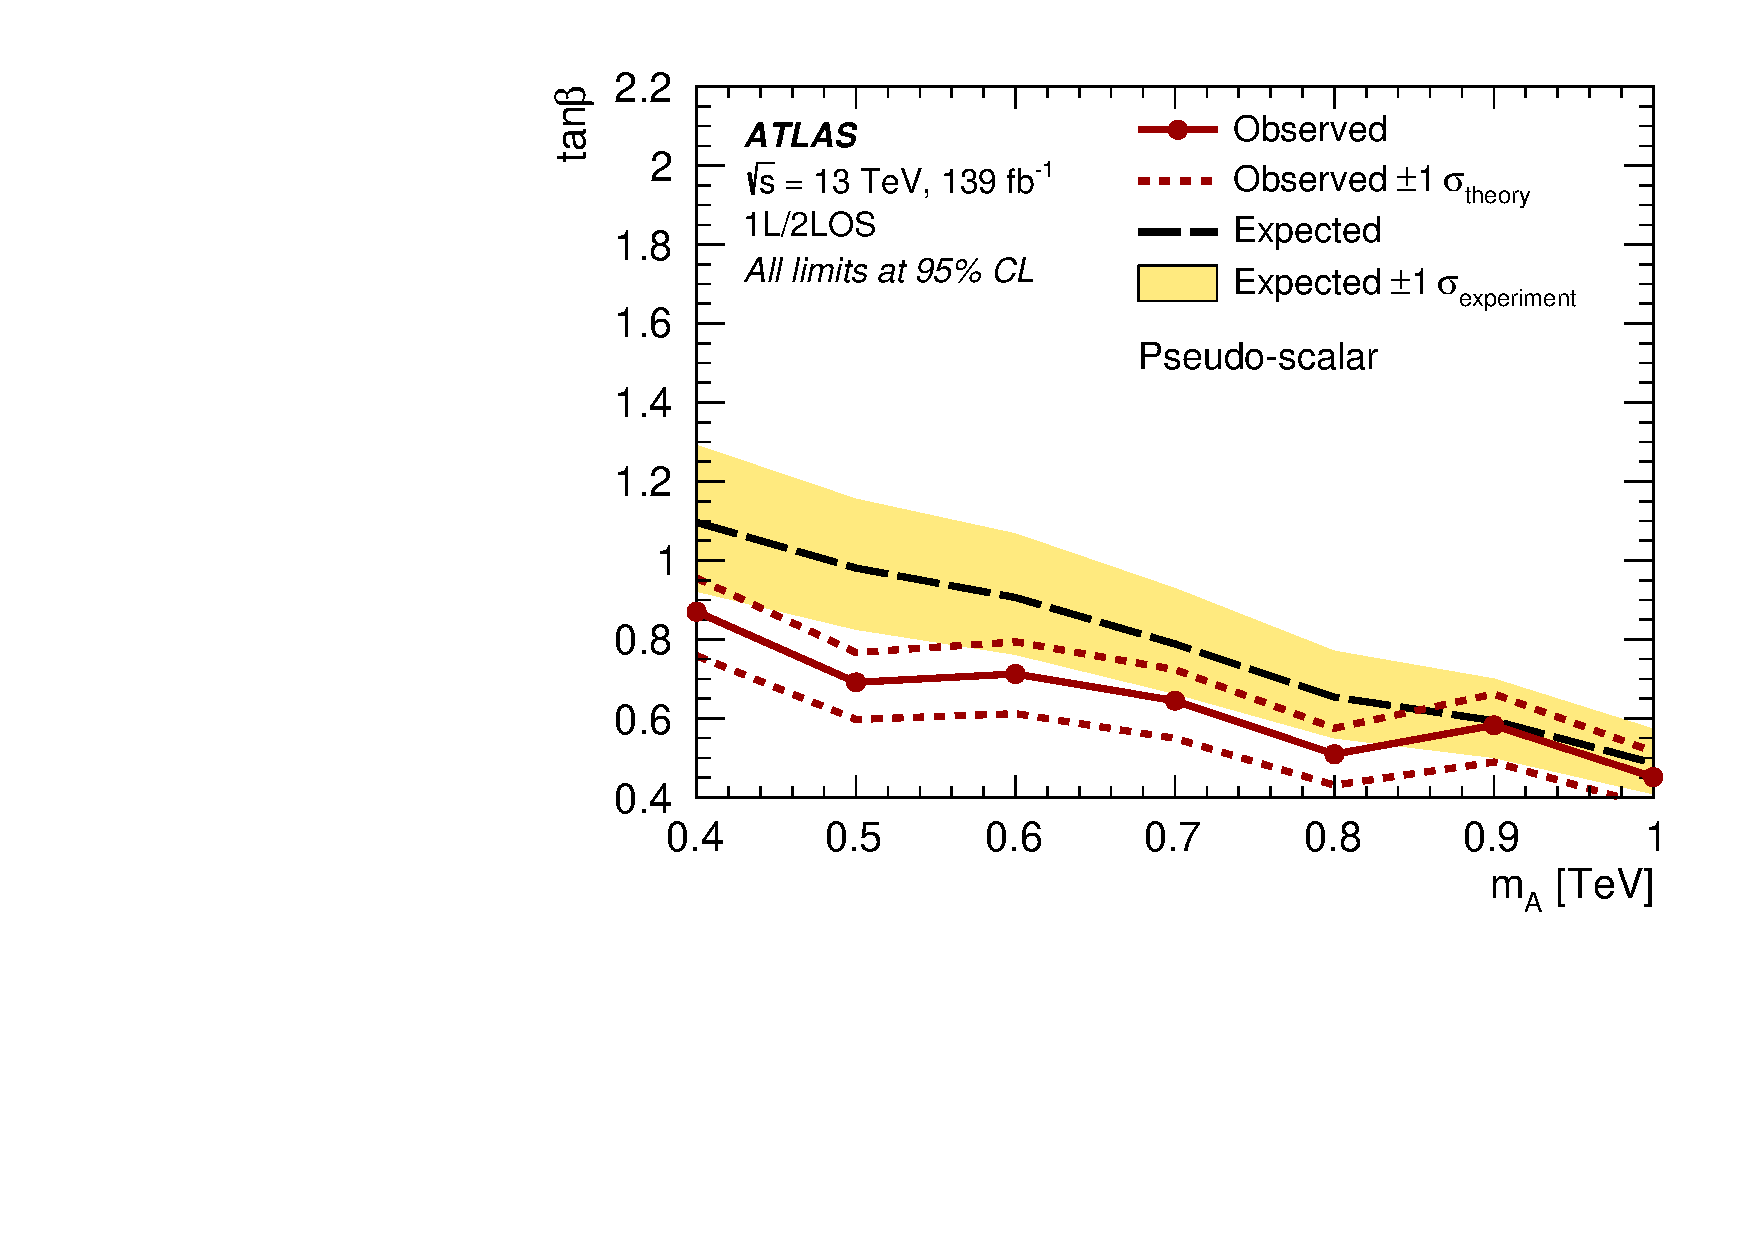
\includegraphics[width=\linewidth]{figures/figures_paper/Data_12fb_ttA_1LOS.pdf}
    \caption{Pseudoscalar $A$ only}
  \end{subfigure}

  \caption{
  Observed and expected exclusion regions at 95\% CL in the 
  $\boldsymbol{(m_{H/A}, \tan\beta)}$ plane in the 2HDM type-II framework 
  for three benchmark scenarios.}
  \label{fig:2D_1LOS}
\end{figure}

In the scenario where both $H$ and $A$ contribute with equal masses, 
the strongest exclusions are obtained at low $\tan\beta$, where the top Yukawa coupling is enhanced. 
The exclusion weakens at larger masses due to the rapidly decreasing production cross section and reduced signal acceptance. 
When only one of the two states is assumed to contribute, the excluded parameter space is correspondingly reduced, reflecting the smaller overall signal yield.

\subsubsection{Combined interpretation with the 2LSS/3L channel}
\label{sec:limits_combined}

The 1L/2LOS analysis is combined with the ATLAS search in the 2LSS/3L final state using a simultaneous profile likelihood fit across all signal and control regions of both analyses. 
The combination is performed within a single statistical model, preserving the full correlation structure of systematic uncertainties.

Experimental uncertainties associated with reconstructed objects are treated as fully correlated between the two channels, while background-specific modelling uncertainties are treated as uncorrelated when appropriate to reflect differences in background composition and estimation strategies. 
This ensures a statistically consistent extraction of limits while accounting for channel-dependent systematic effects.

A comparison of the fitted signal strengths and significances between the individual channels and the combined fit is shown in Figures~\ref{fig:combination_mu} and~\ref{fig:combination_significance}. 
No statistically significant excess is observed.

\begin{figure} 
    \centering 
    \begin{subfigure}[t]{0.49\textwidth} 
        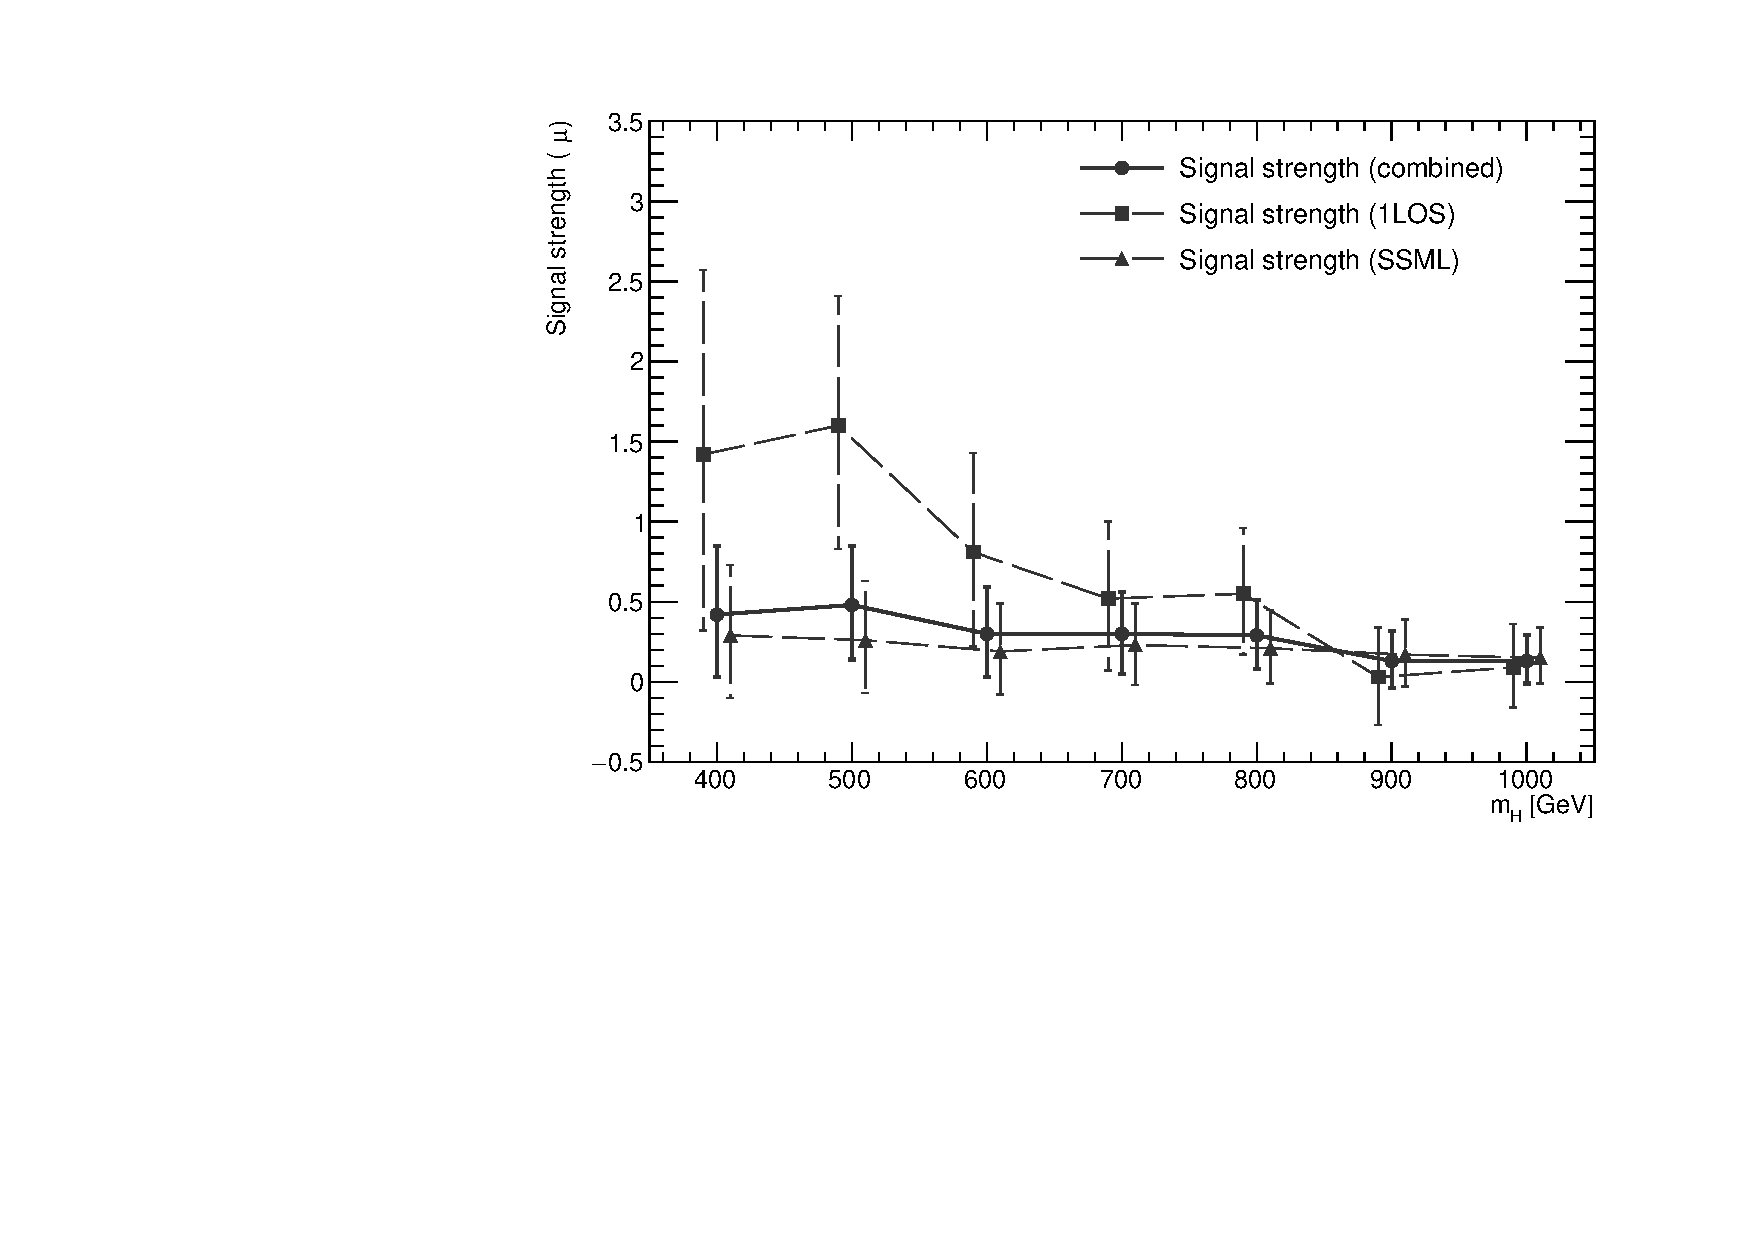
\includegraphics[width=1 \textwidth]{figures/combined_fit/mu_comp.pdf} 
        \caption{Signal strength} 
    \end{subfigure} 
    \caption{\label{fig:combination_mu}Comparison of the fitted signal strength among the combined fit and each channel fit.} 
\end{figure}

\begin{figure} 
    \centering 
    \begin{subfigure}[t]{0.49\textwidth} 
        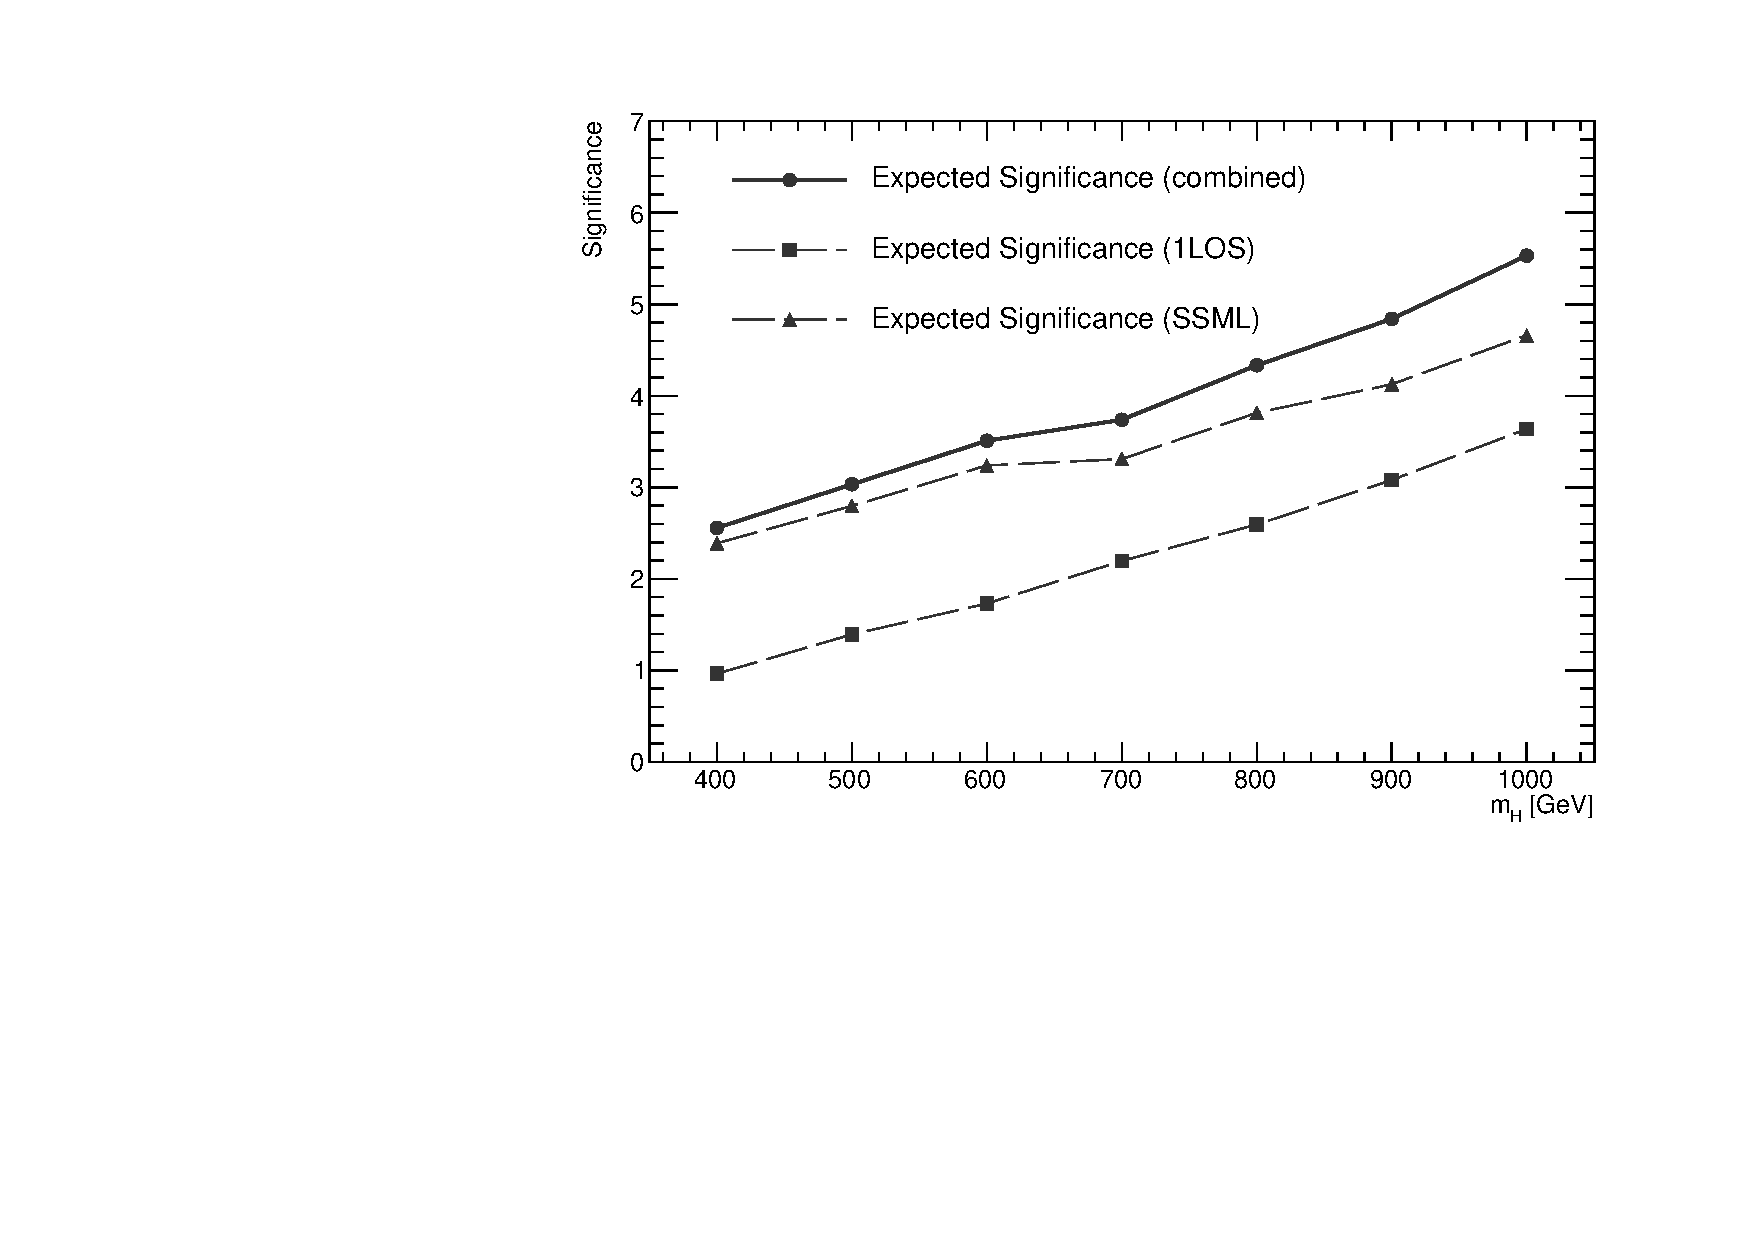
\includegraphics[width=1 \textwidth]{figures/combined_fit/sig_comp_exp.pdf} 
        \caption{Expected significance} 
    \end{subfigure} 
    \begin{subfigure}[t]{0.49\textwidth} 
        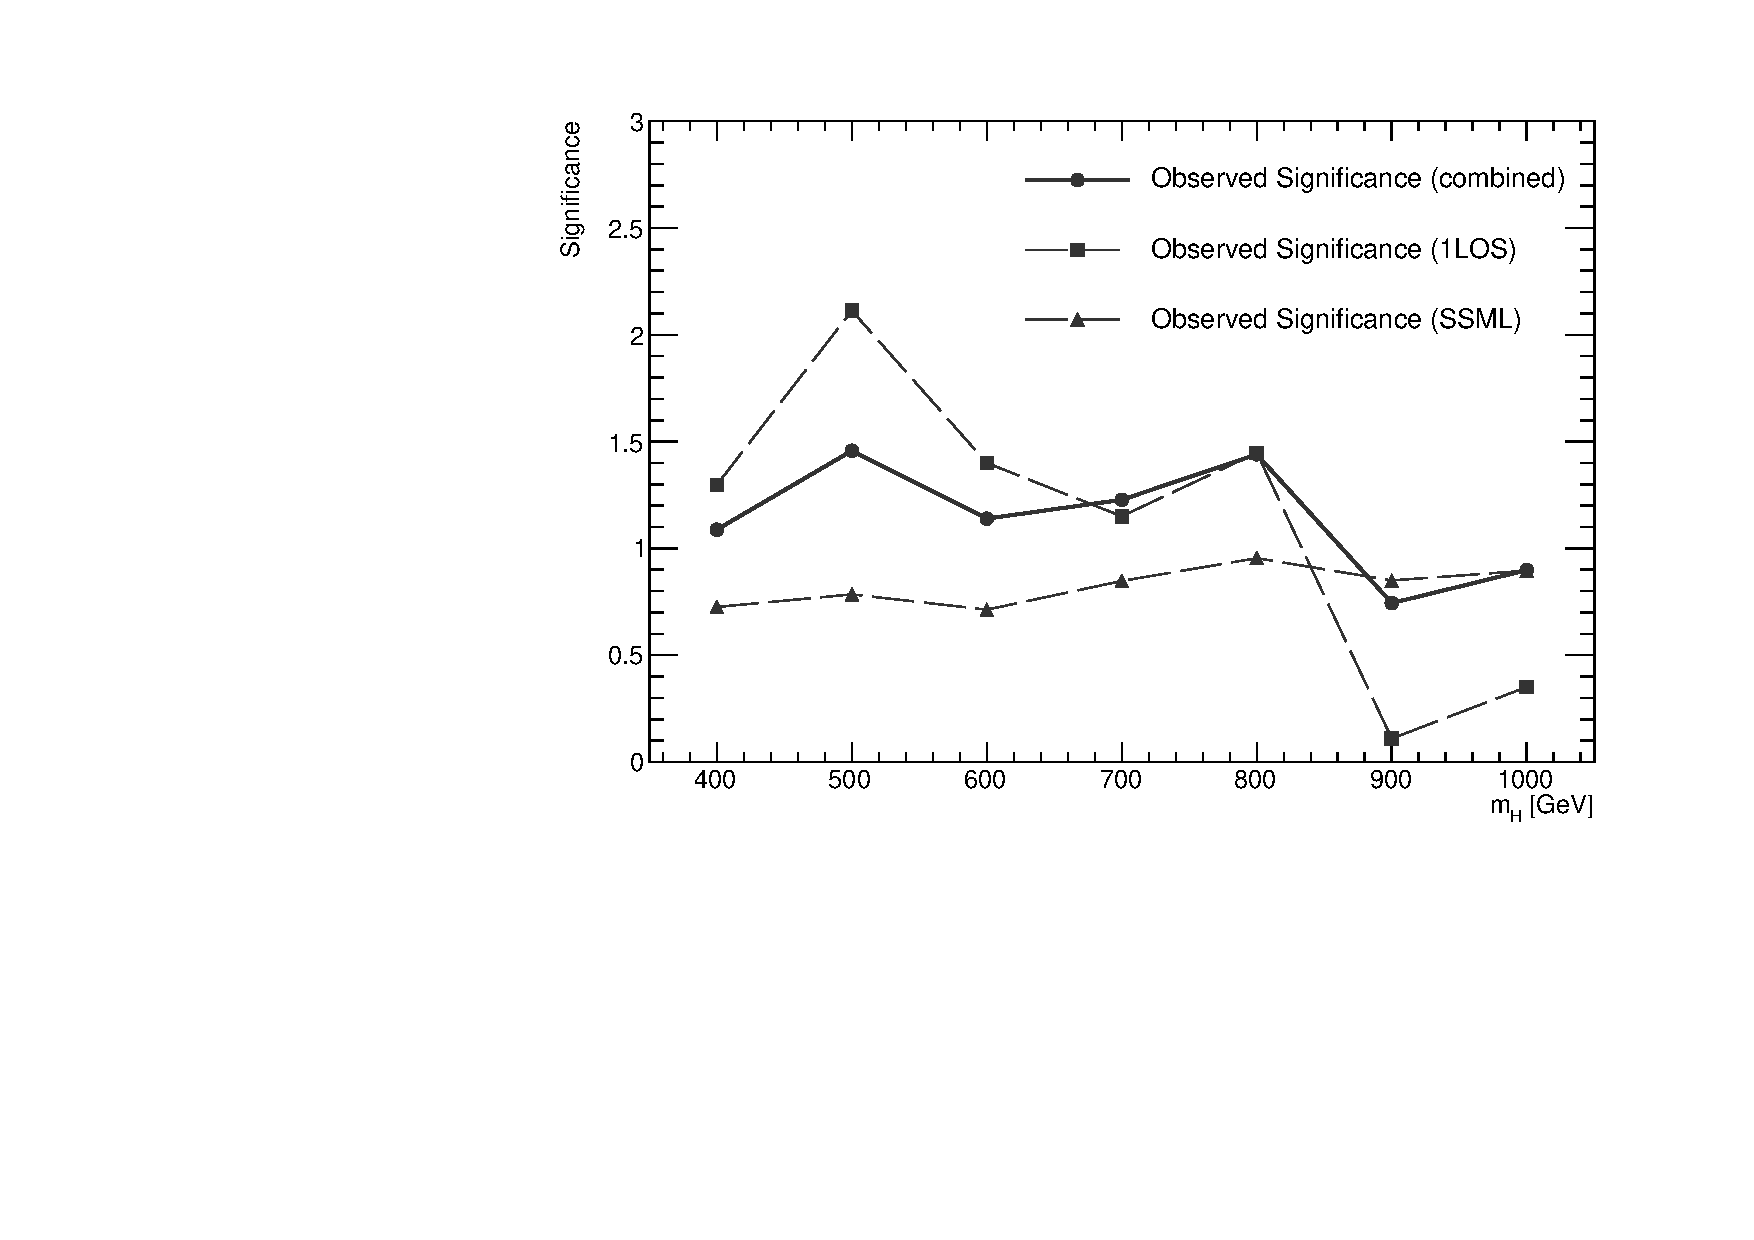
\includegraphics[width=1 
        \textwidth]{figures/combined_fit/sig_comp_obs.pdf} 
        \caption{Observed significance} 
    \end{subfigure} 
    \caption{\label{fig:combination_significance}Comparison of the expected (left) and observed (right) significance among the combined fit and each channel fit.} 
\end{figure} 

The expected and observed 95\% CL upper limits on $\sigma(pp \to t\bar{t}H/A) \times \mathcal{B}(H/A \to t\bar{t})$
from the combined fit are shown in Figure~\ref{fig:combination_limit_1}. 
The observed (expected) upper limits range from 14 (9.4) fb at $m_{H/A}=400$~GeV to 5.0 (3.8) fb at $m_{H/A}=1000$~GeV.
For comparison, the expected limits from the individual 1L/2LOS and 2LSS/3L channels are also displayed.

\begin{figure}[htbp!]
    \centering
    \begin{subfigure}[t]{0.49\textwidth}
      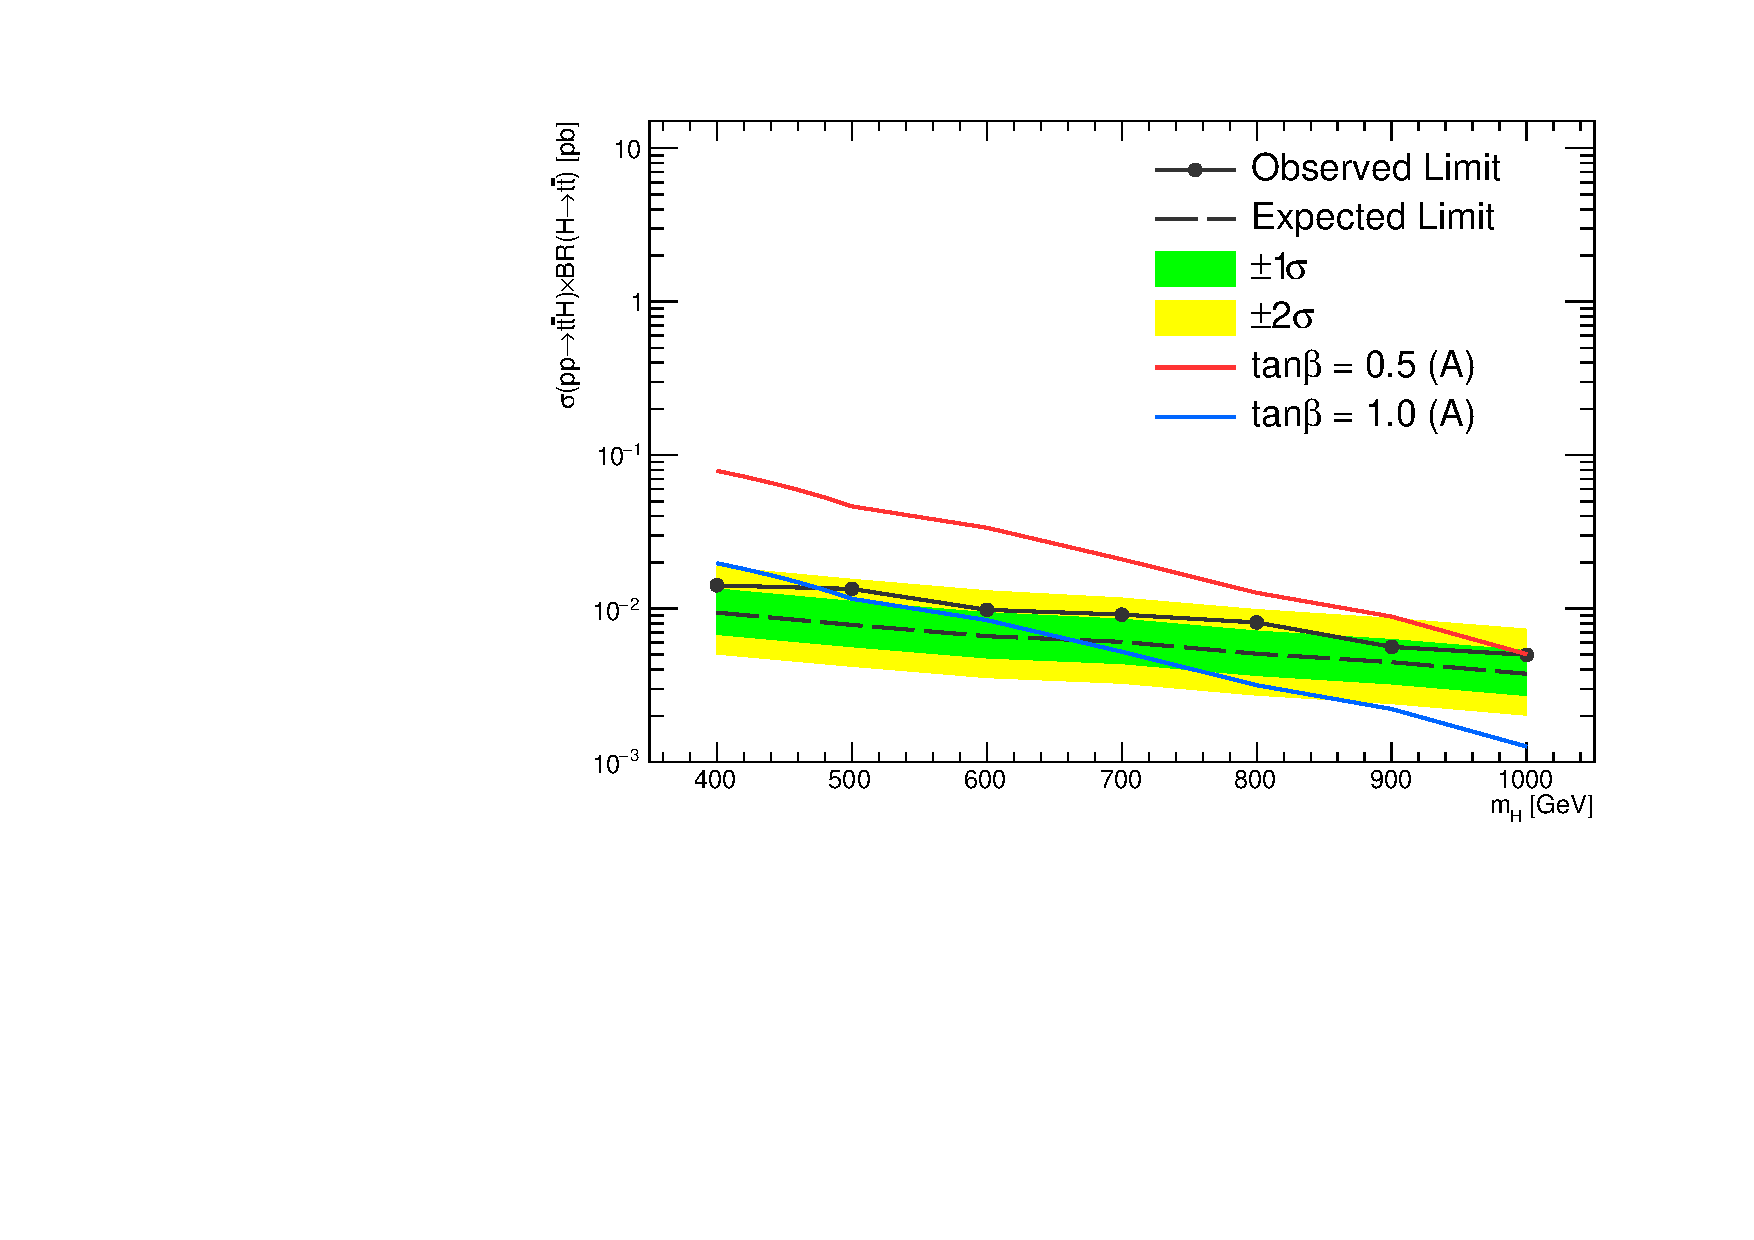
\includegraphics[width=\linewidth]{figures/combined_fit/lim_combined.pdf}
      \caption{Expected and observed limits}
    \end{subfigure}
    \begin{subfigure}[t]{0.49\textwidth}
      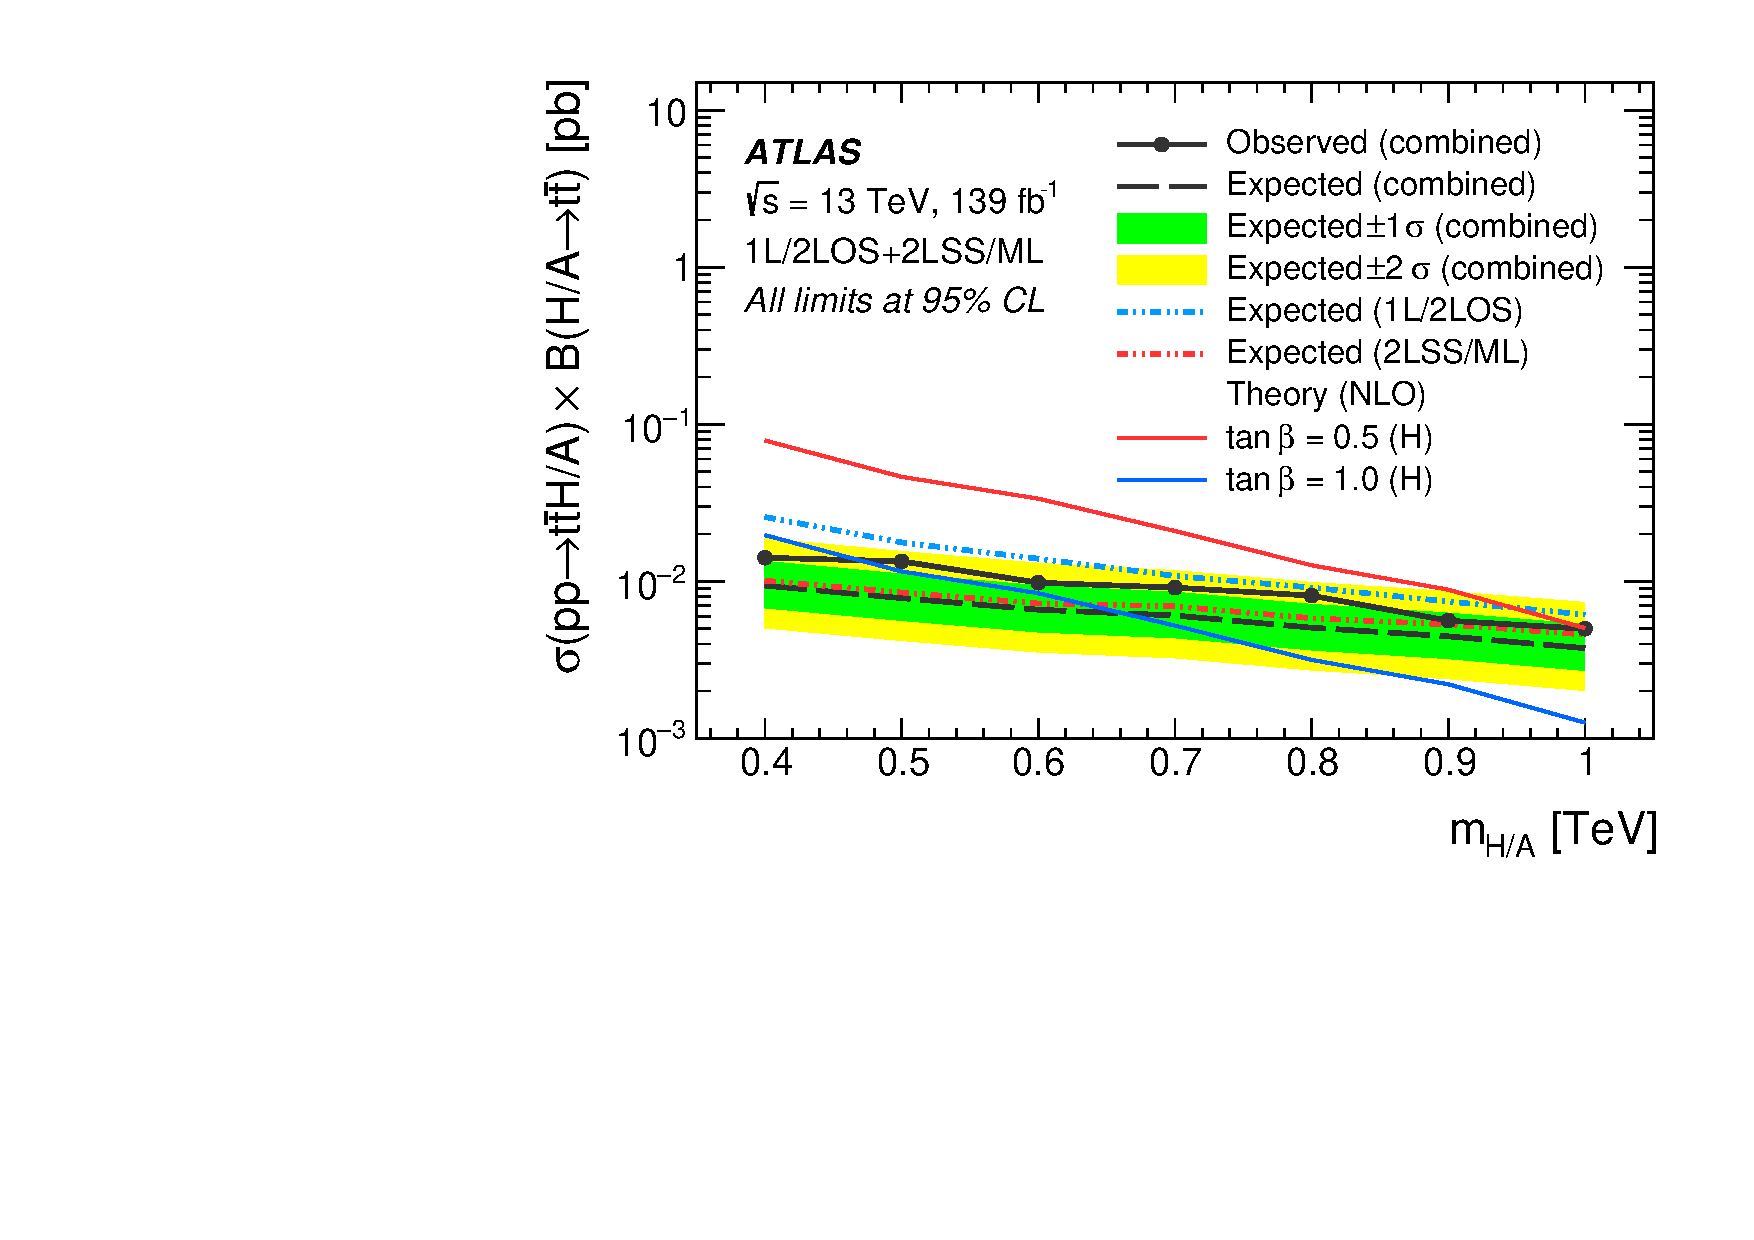
\includegraphics[width=\linewidth]{figures/figures_paper/lim_combined_with_individual_exp.pdf}
      \caption{Comparison with individual channels}
    \end{subfigure}
    \caption{\label{fig:combination_limit_1}
    Observed and expected 95\% CL upper limits on 
    $\boldsymbol{\sigma(pp \to t\bar{t}H/A) \times \mathcal{B}(H/A \to t\bar{t})}$ 
    as a function of $\boldsymbol{m_{H/A}}$ from the combined fit.}
\end{figure}

The combination improves the sensitivity across the full mass range considered. 
The gain arises from the complementary signal acceptance and background composition of the two channels. 
The 1L/2LOS channel provides strong sensitivity in high jet and $b$-tag multiplicity regions dominated by $t\bar{t}$+jets backgrounds, 
while the 2LSS/3L channel benefits from a lower background environment and reduced contamination from mis-modelled $t\bar{t}$ processes. 
As a result, the combined observed limits are improved by up to 19\% relative to the most sensitive individual channel at $m_{H/A} = 900$ GeV, with the expected limit improved by up to 18\%.

The combined limits are translated into exclusion regions in the $(m_{H/A}, \tan\beta)$ parameter plane of the 2HDM type-II. 
Figure~\ref{fig:combination_2Dplots} shows the observed and expected exclusions for three benchmark scenarios:
(i) $m_H = m_A$ with both states contributing,
(ii) only the scalar $H$, and
(iii) only the pseudoscalar $A$ contributing to the final state.

\begin{figure}[htbp!]
  \centering
  \begin{subfigure}[t]{0.49\textwidth}
    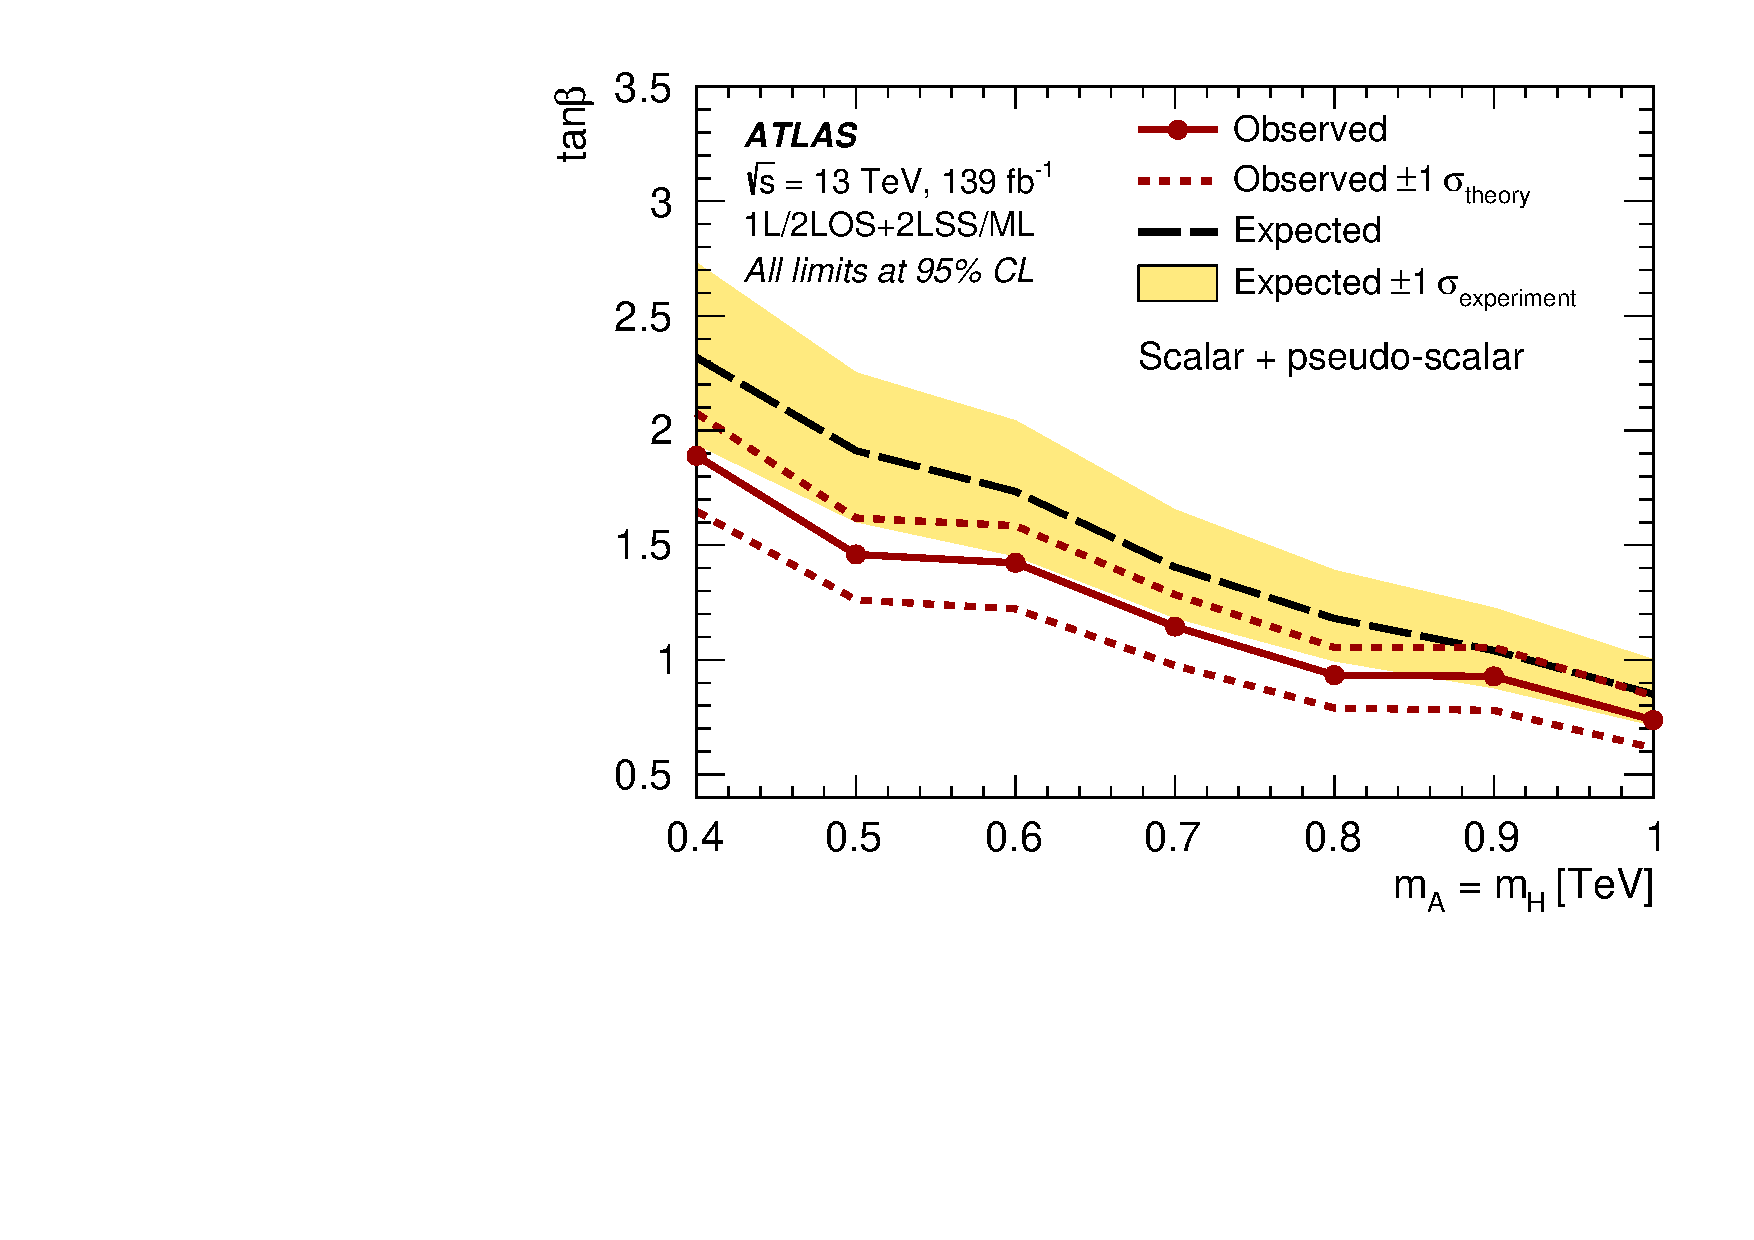
\includegraphics[width=\linewidth]{figures/figures_paper/Data_12fb_All_combined.pdf}
    \caption{$m_H = m_A$, both contribute}
  \end{subfigure}
  \hfill
  \begin{subfigure}[t]{0.49\textwidth}
    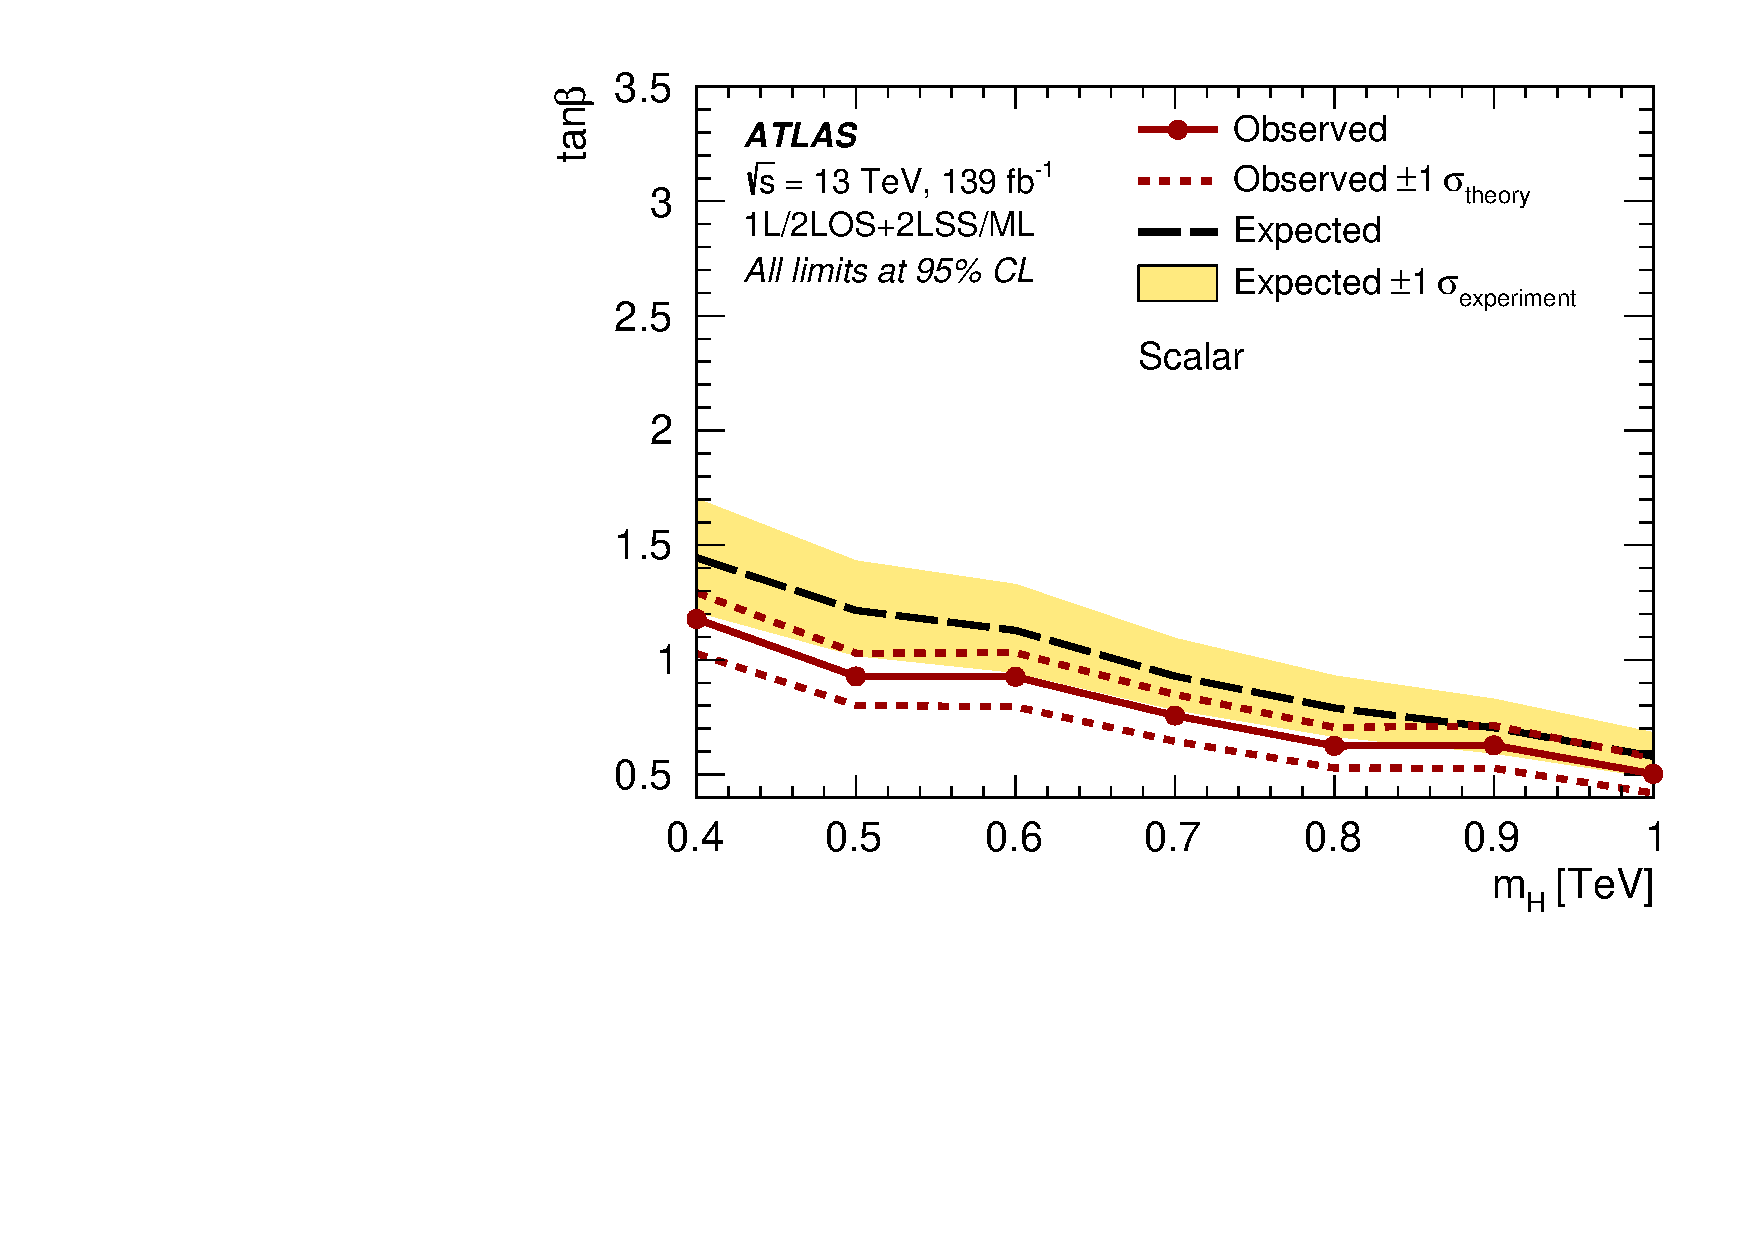
\includegraphics[width=\linewidth]{figures/figures_paper/Data_12fb_ttH_combined.pdf}
    \caption{Scalar $H$ only}
  \end{subfigure}

  \vspace{0.4cm}

  \begin{subfigure}[t]{0.49\textwidth}
    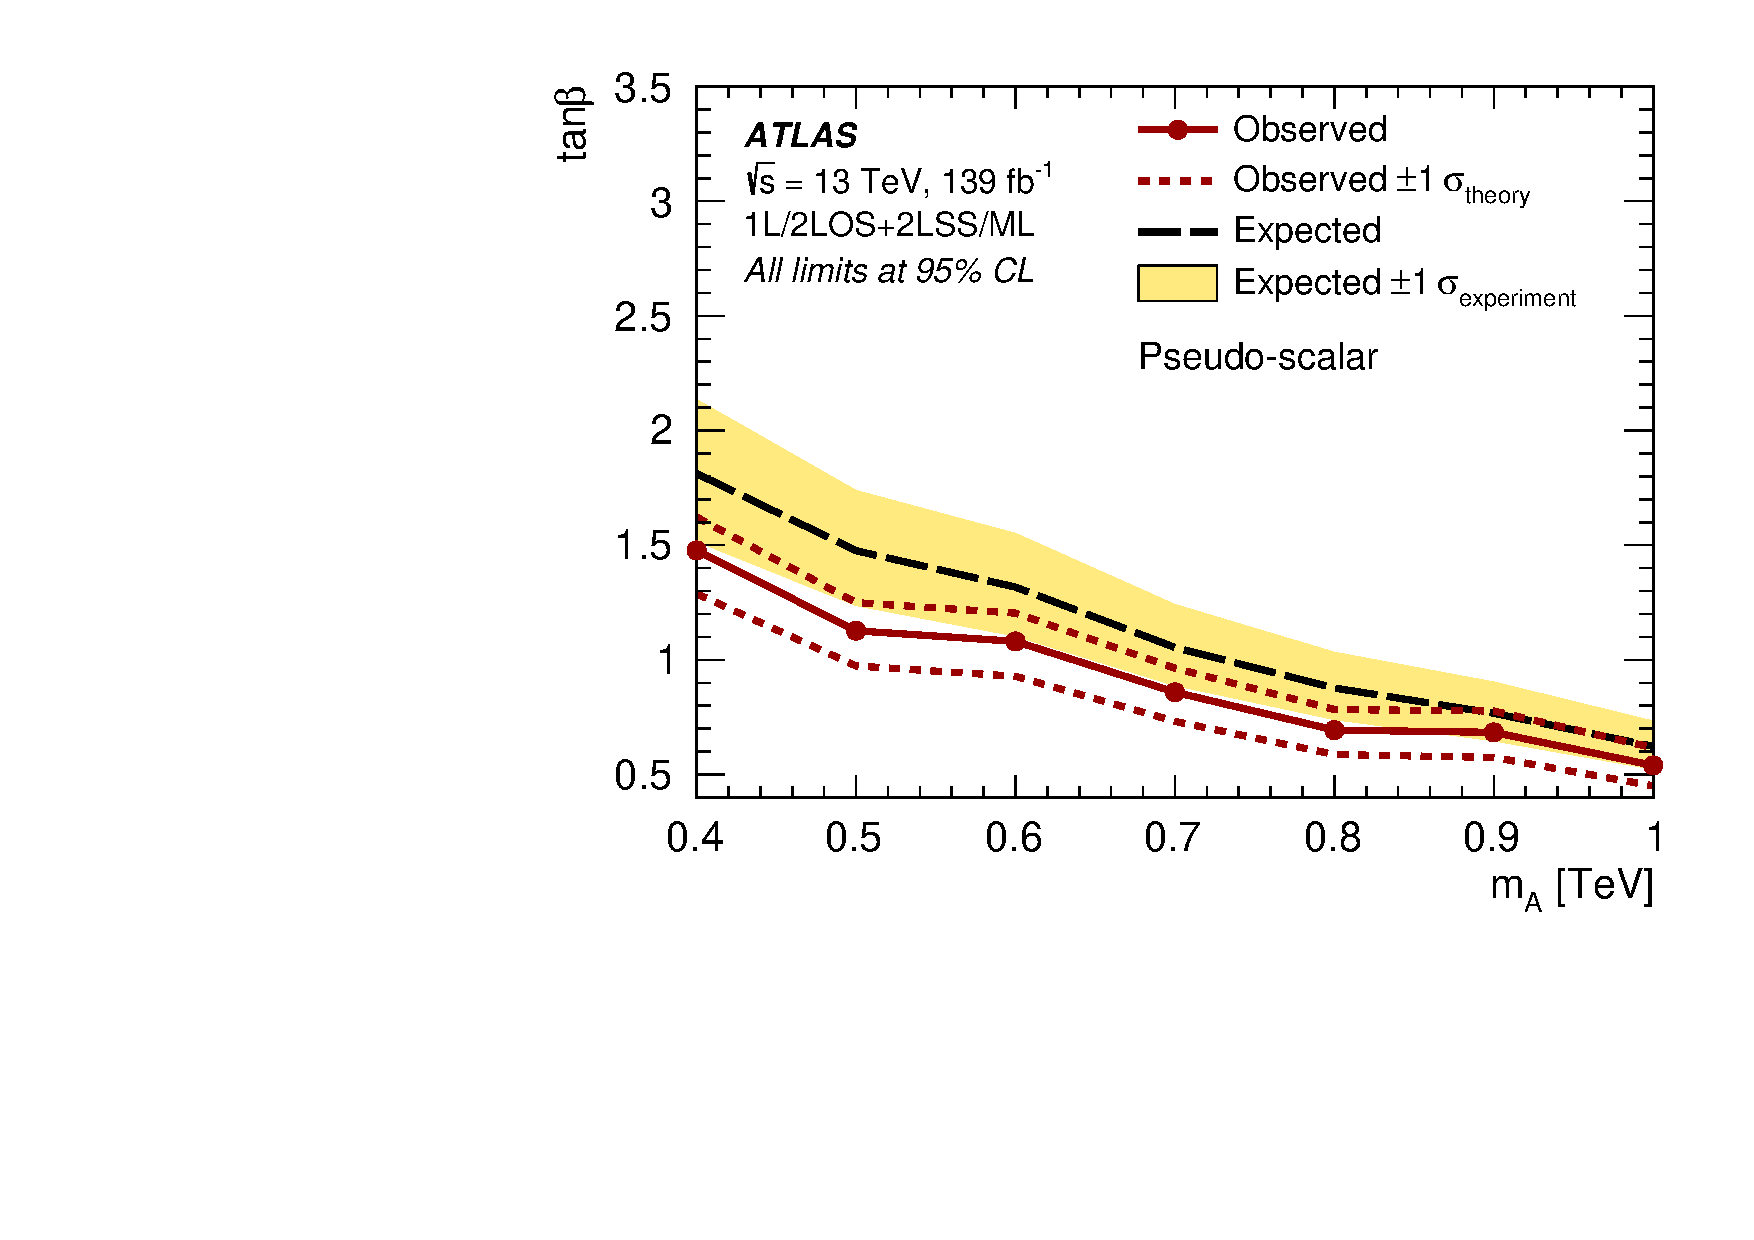
\includegraphics[width=\linewidth]{figures/figures_paper/Data_12fb_ttA_combined.pdf}
    \caption{Pseudoscalar $A$ only}
  \end{subfigure}

  \caption{
  Observed and expected exclusion regions at 95\% CL in the 
  $\boldsymbol{(m_{H/A}, \tan\beta)}$ plane from the combined fit of the 
  1L/2LOS and 2LSS/3L channels in the 2HDM type-II framework 
  for three benchmark scenarios.}
  \label{fig:combination_2Dplots}
\end{figure}

Compared to the single-channel interpretation, the excluded parameter space is extended in all three benchmark scenarios, 
with the most significant improvement observed in the low-$\tan\beta$ region where the production cross section is largest. 
The qualitative exclusion pattern remains consistent with that observed in the individual analyses, 
while the combined fit provides the most stringent constraints within the mass range studied.

\subsection{Interpretation in the sgluon model}
\label{sec:limits_sgluon}

In addition to the 2HDM interpretation, the results are interpreted in the context of a simplified model containing scalar colour-octet particles ($S_8$), commonly referred to as sgluons. 
In this scenario, sgluons are pair-produced via the strong interaction and subsequently decay into top-quark pairs, leading to a $t\bar{t}t\bar{t}$ final state.

The same analysis strategy is employed to derive upper limits on the 
$S_8 S_8 \rightarrow t\bar{t}t\bar{t}$ production cross section. 
The limits are first extracted separately in the 1L/2LOS and 2LSS/ML final states. 
For mass points with $m_{S_8} \leq 1$~TeV, the $m_{H/A}$-parameterised multivariate classifiers (GNN for 1L/2LOS and BDT for 2LSS/ML) are evaluated at $m_{S_8} = m_{H/A}$. 
At each mass point, the binning of the fitted distributions is chosen to match that used in the $H/A$ analysis. 
For $m_{S_8} > 1$~TeV, the classifiers and binning corresponding to $m_{H/A}=1$~TeV are adopted.

The expected and observed 95\% CL upper limits on the $S_8 S_8 \rightarrow t\bar{t}t\bar{t}$ production cross section obtained in the two individual final states are shown in Figure~\ref{fig:sgluon_individual}.

\begin{figure}[htbp!]
 \centering
 \begin{subfigure}[t]{0.49\textwidth}
  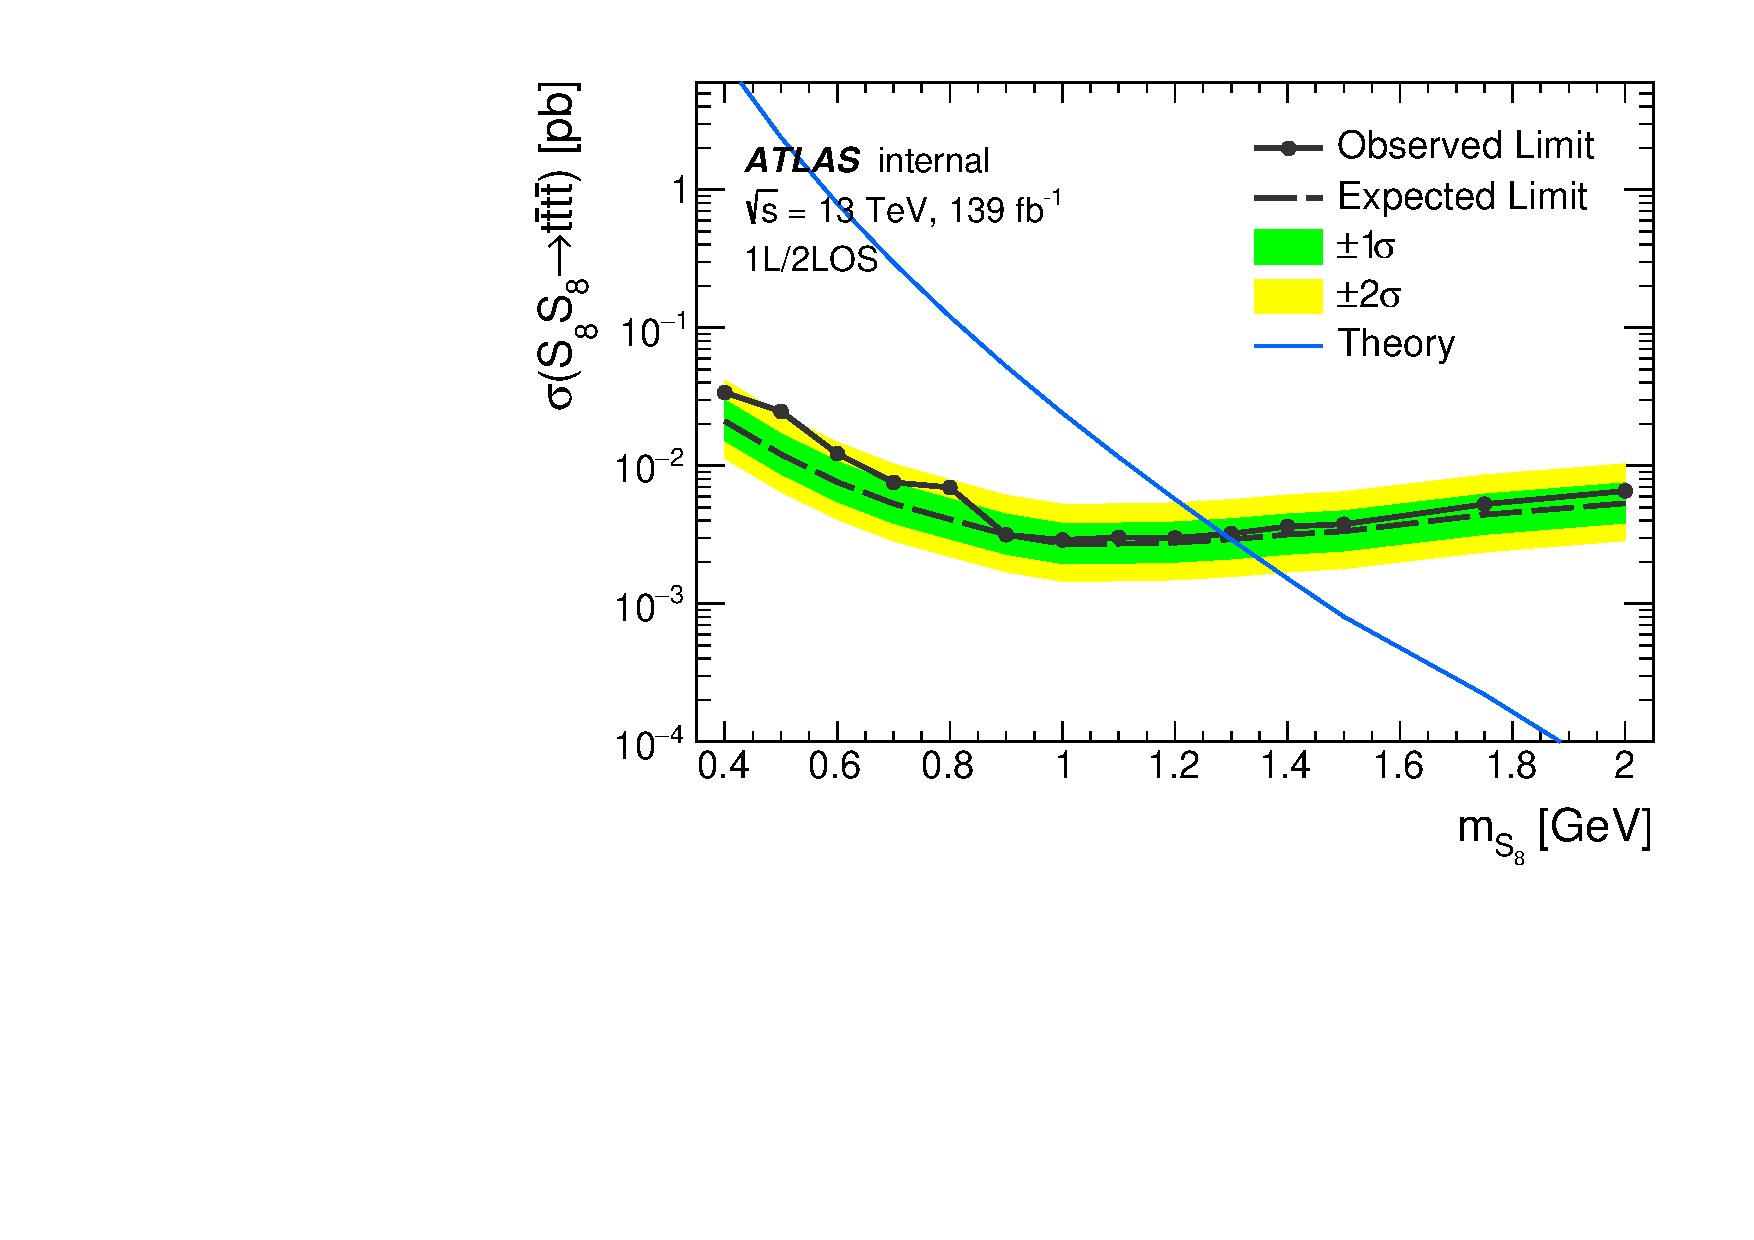
\includegraphics[width=\linewidth]{figures/sgluon_limits/lim_1LOS.pdf}
  \caption{1L/2LOS}
 \end{subfigure}
 \hfill
 \begin{subfigure}[t]{0.49\textwidth}
  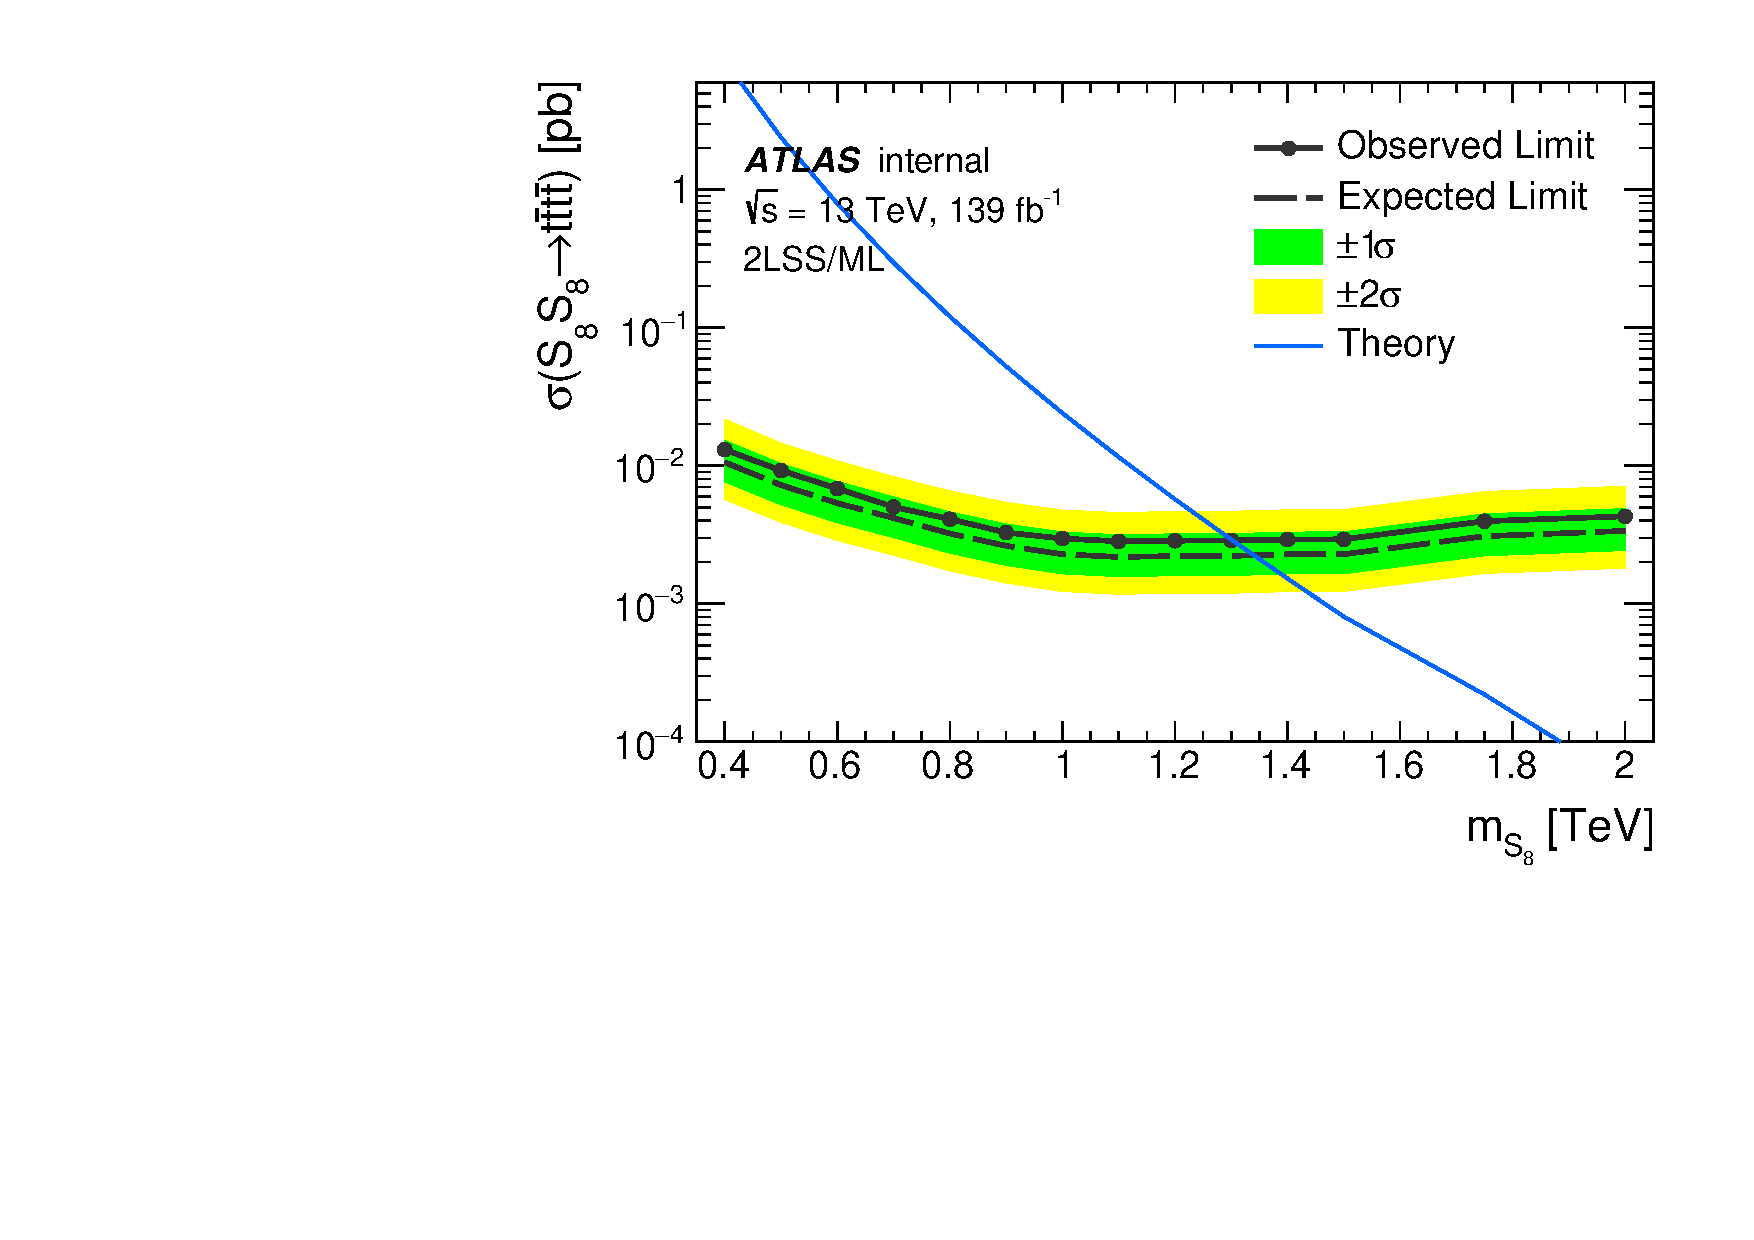
\includegraphics[width=\linewidth]{figures/sgluon_limits/lim_SSML.pdf}
  \caption{2LSS/ML}
 \end{subfigure}
 \caption{\label{fig:sgluon_individual}
 Observed and expected 95\% CL upper limits on the cross section for 
 $\boldsymbol{S_8 S_8 \rightarrow t\bar{t}t\bar{t}}$ production 
 as a function of $\boldsymbol{m_{S_8}}$ in the 1L/2LOS (left) and 2LSS/ML (right) final states.}
\end{figure}

The two final states are then combined using a simultaneous profile likelihood fit, treating systematic uncertainties consistently as described in Section~\ref{sec:limits_combined}. 
The resulting 95\% CL upper limits on the $S_8 S_8 \rightarrow t\bar{t}t\bar{t}$ production cross section are shown in Figure~\ref{fig:sgluon_combination}. 
For comparison, the expected limits from the individual analyses are also displayed.

\begin{figure}[htbp!]
 \centering
 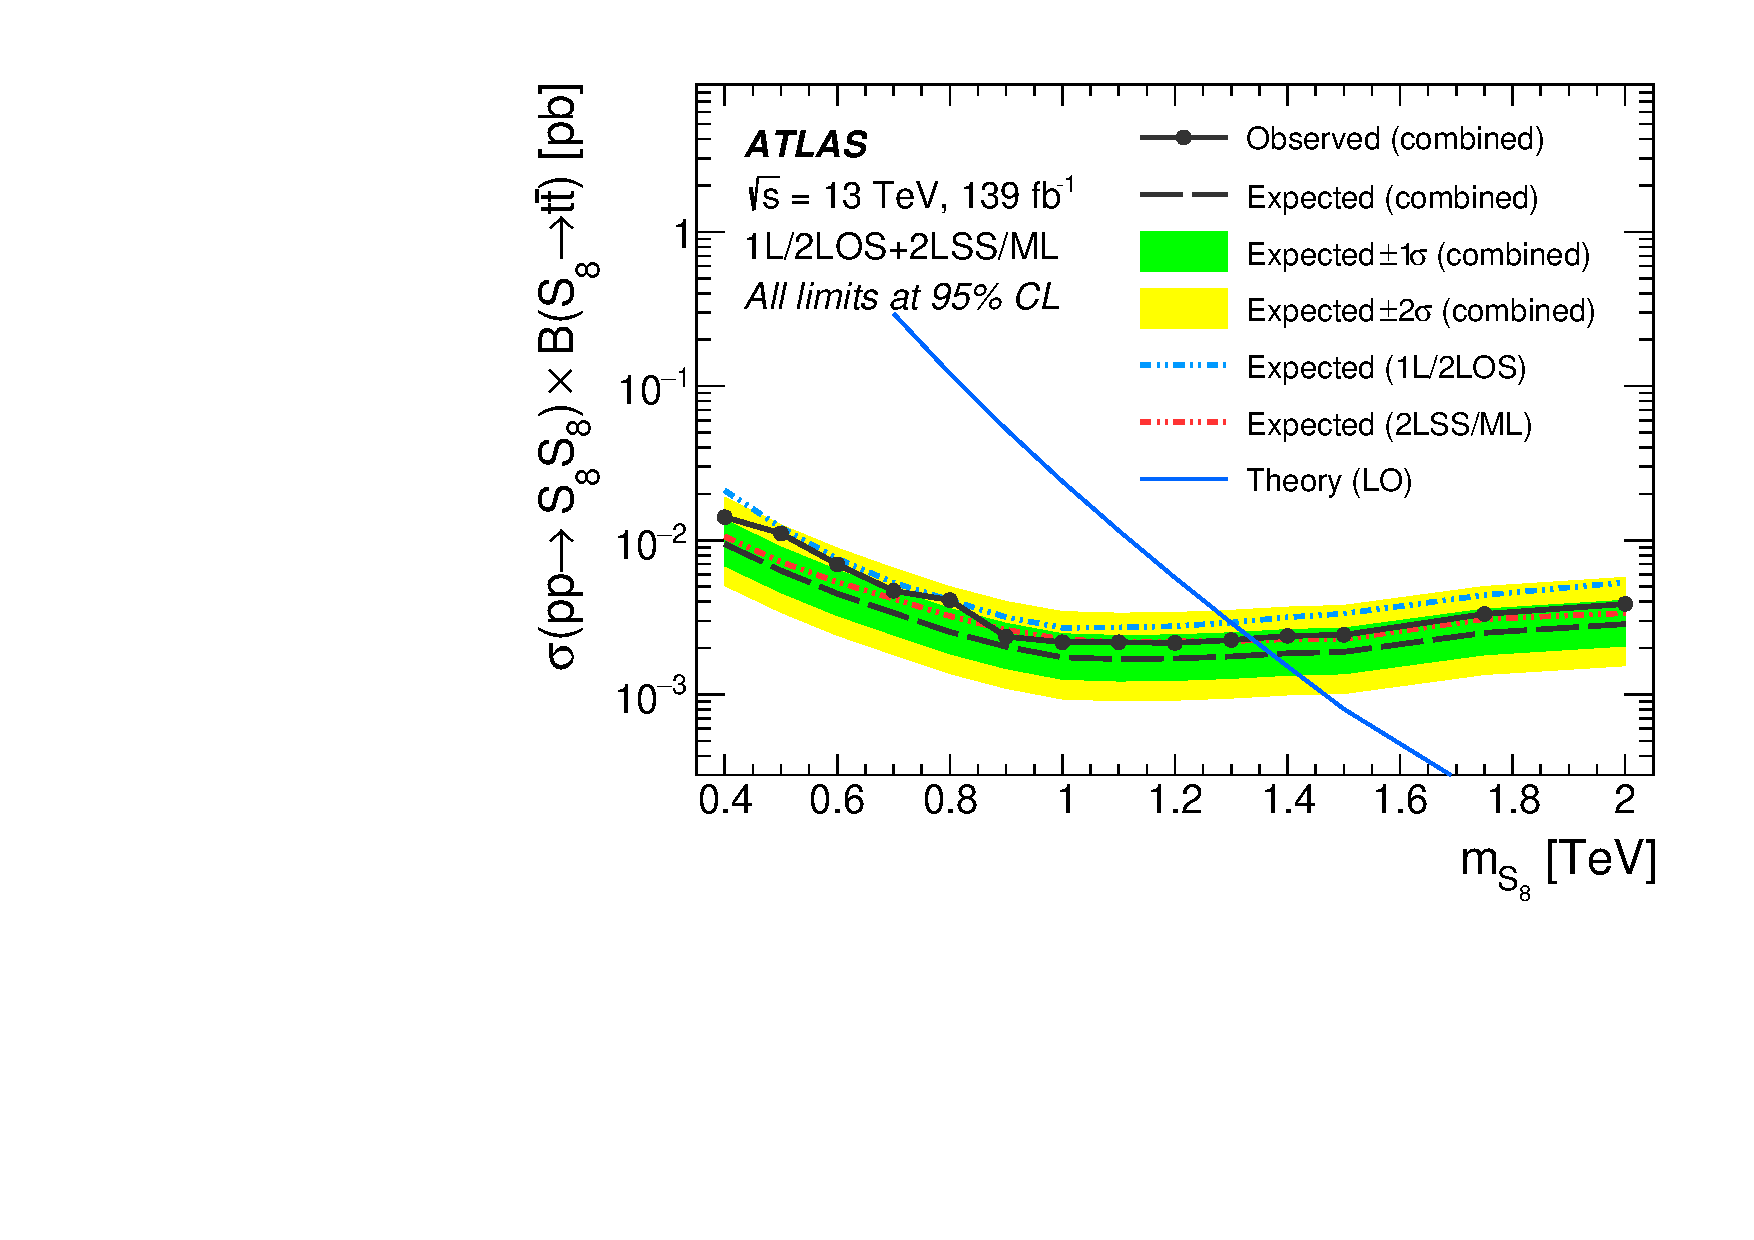
\includegraphics[width=0.6\textwidth]{figures/figures_paper/sgluon_lim_combined_with_individual_exp.pdf}
 \caption{\label{fig:sgluon_combination}
 Observed and expected 95\% CL upper limits on the 
 $\boldsymbol{S_8 S_8 \rightarrow t\bar{t}t\bar{t}}$ production cross section 
 as a function of $\boldsymbol{m_{S_8}}$ from the combination of the 1L/2LOS and 2LSS/ML final states. 
 The predicted production cross section from Ref.~\cite{Darm__2021} is shown for comparison.}
\end{figure}

For $m_{S_8} \leq 1$~TeV, the behaviour of the limits closely follows that observed in the $t\bar{t}H/A \rightarrow t\bar{t}t\bar{t}$ interpretation, 
with an improvement of up to 26\% in the expected sensitivity when combining the two final states compared to using the 2LSS/ML channel alone. 
For $m_{S_8} > 1$~TeV, the limits slightly weaken due to the use of classifiers optimised for $m_{H/A}=1$~TeV.

By comparing the observed limits with the theoretical prediction, 
sgluon masses up to approximately 1.3~TeV are excluded at 95\% CL.